% Initial and revised submissions should be 12 point; this will be removed in the final version.
%\documentclass[12pt]{TD-CJS}
\documentclass{article}

% Initial and revised submissions should also be double spaced.  This command will be removed in the final version.
%\renewcommand{\baselinestretch}{2}

\usepackage{latexsym}
\usepackage{amsmath}
\usepackage{amsfonts}
\usepackage{amssymb}
\usepackage{psfrag}
\usepackage{graphicx}
\usepackage[dvipsnames]{xcolor}
\usepackage{url}
\usepackage{float}
\usepackage[margin=1in]{geometry}
% header.tex
% this is where you load pacakges, specify custom formats, etc.

% \usepackage{changepage}
\usepackage{amsmath,amsthm,amssymb,amsfonts}
\usepackage{mathtools}
\usepackage{bbm}
% enumitem for custom lists
\usepackage{enumitem}
% Load dsfont this to get proper indicator function (bold 1) with \mathds{1}:
\usepackage{dsfont}
\usepackage{centernot}
\usepackage{appendix}

% set up graphics
\usepackage{graphicx}
\DeclareGraphicsExtensions{.pdf,.png,.jpg}
\graphicspath{ {fig/} }
% defs.tex
% this is where you define custom notation, commands, etc.

\DeclareMathOperator*{\argmax}{arg\,max}
\DeclareMathOperator*{\argmin}{arg\,min}
\DeclareMathOperator*{\del}{\nabla}

%%
% full alphabets of different styles
%%

% bf series
\def\bfA{\mathbf{A}}
\def\bfB{\mathbf{B}}
\def\bfC{\mathbf{C}}
\def\bfD{\mathbf{D}}
\def\bfE{\mathbf{E}}
\def\bfF{\mathbf{F}}
\def\bfG{\mathbf{G}}
\def\bfH{\mathbf{H}}
\def\bfI{\mathbf{I}}
\def\bfJ{\mathbf{J}}
\def\bfK{\mathbf{K}}
\def\bfL{\mathbf{L}}
\def\bfM{\mathbf{M}}
\def\bfN{\mathbf{N}}
\def\bfO{\mathbf{O}}
\def\bfP{\mathbf{P}}
\def\bfQ{\mathbf{Q}}
\def\bfR{\mathbf{R}}
\def\bfS{\mathbf{S}}
\def\bfT{\mathbf{T}}
\def\bfU{\mathbf{U}}
\def\bfV{\mathbf{V}}
\def\bfW{\mathbf{W}}
\def\bfX{\mathbf{X}}
\def\bfY{\mathbf{Y}}
\def\bfZ{\mathbf{Z}}

% bb series
\def\bbA{\mathbb{A}}
\def\bbB{\mathbb{B}}
\def\bbC{\mathbb{C}}
\def\bbD{\mathbb{D}}
\def\bbE{\mathbb{E}}
\def\bbF{\mathbb{F}}
\def\bbG{\mathbb{G}}
\def\bbH{\mathbb{H}}
\def\bbI{\mathbb{I}}
\def\bbJ{\mathbb{J}}
\def\bbK{\mathbb{K}}
\def\bbL{\mathbb{L}}
\def\bbM{\mathbb{M}}
\def\bbN{\mathbb{N}}
\def\bbO{\mathbb{O}}
\def\bbP{\mathbb{P}}
\def\bbQ{\mathbb{Q}}
\def\bbR{\mathbb{R}}
\def\bbS{\mathbb{S}}
\def\bbT{\mathbb{T}}
\def\bbU{\mathbb{U}}
\def\bbV{\mathbb{V}}
\def\bbW{\mathbb{W}}
\def\bbX{\mathbb{X}}
\def\bbY{\mathbb{Y}}
\def\bbZ{\mathbb{Z}}

% cal series
\def\calA{\mathcal{A}}
\def\calB{\mathcal{B}}
\def\calC{\mathcal{C}}
\def\calD{\mathcal{D}}
\def\calE{\mathcal{E}}
\def\calF{\mathcal{F}}
\def\calG{\mathcal{G}}
\def\calH{\mathcal{H}}
\def\calI{\mathcal{I}}
\def\calJ{\mathcal{J}}
\def\calK{\mathcal{K}}
\def\calL{\mathcal{L}}
\def\calM{\mathcal{M}}
\def\calN{\mathcal{N}}
\def\calO{\mathcal{O}}
\def\calP{\mathcal{P}}
\def\calQ{\mathcal{Q}}
\def\calR{\mathcal{R}}
\def\calS{\mathcal{S}}
\def\calT{\mathcal{T}}
\def\calU{\mathcal{U}}
\def\calV{\mathcal{V}}
\def\calW{\mathcal{W}}
\def\calX{\mathcal{X}}
\def\calY{\mathcal{Y}}
\def\calZ{\mathcal{Z}}

\def\bfTheta{\mathbf{\Theta}}


%%%%%%%%%%%%%%%%%%%%%%%%%%%%%%%%%%%%%%%%%%%%%%%%%%%%%%%%%%
% text short-cuts
\def\iid{i.i.d.\ } %i.i.d.
\def\ie{i.e.\ }
\def\eg{e.g.\ }
\def\Polya{P\'{o}lya\ }
%%%%%%%%%%%%%%%%%%%%%%%%%%%%%%%%%%%%%%%%%%%%%%%%%%%%%%%%%%

%%%%%%%%%%%%%%%%%%%%%%%%%%%%%%%%%%%%%%%%%%%%%%%%%%%%%%%%%%
% quasi-universal probabilistic and mathematical notation
% my preferences (modulo publication conventions, and clashes like random vectors):
%   vectors: bold, lowercase
%   matrices: bold, uppercase
%   operators: blackboard (e.g., \mathbb{E}), uppercase
%   sets, spaces: calligraphic, uppercase
%   random variables: normal font, uppercase
%   deterministic quantities: normal font, lowercase
%%%%%%%%%%%%%%%%%%%%%%%%%%%%%%%%%%%%%%%%%%%%%%%%%%%%%%%%%%

% operators
\def\P{\bbP} %fundamental probability
\def\E{\bbE} %expectation
% conditional expectation
\DeclarePairedDelimiterX\bigCond[2]{[}{]}{#1 \;\delimsize\vert\; #2}
\newcommand{\conditional}[3][]{\bbE_{#1}\bigCond*{#2}{#3}}
\def\Law{\mathcal{L}} %law; this is by convention in the literature
\def\indicator{\mathds{1}} % indicator function

% sets and groups
\def\borel{\calB} %Borel sets
\def\sigAlg{\calA} %sigma-algebra
\def\filtration{\calF} %filtration
\def\grp{\calG} %group

% binary relations
\def\condind{{\perp\!\!\!\perp}} %independence/conditional independence
\def\equdist{\stackrel{\text{\rm\tiny d}}{=}} %equal in distribution
\def\equas{\stackrel{\text{\rm\tiny a.s.}}{=}} %euqal amost surely
\def\simiid{\sim_{\mbox{\tiny iid}}} %sampled i.i.d

% common vectors and matrices
\def\onevec{\mathbf{1}}
\def\iden{\mathbf{I}} % identity matrix
\def\supp{\text{\rm supp}}

% misc
% floor and ceiling
\DeclarePairedDelimiter{\ceilpair}{\lceil}{\rceil}
\DeclarePairedDelimiter{\floor}{\lfloor}{\rfloor}
\newcommand{\argdot}{{\,\vcenter{\hbox{\tiny$\bullet$}}\,}} %generic argument dot
%%%%%%%%%%%%%%%%%%%%%%%%%%%%%%%%%%%%%%%%%%%%%%%%%%%%%%%%%%

%%%%%%%%%%%%%%%%%%%%%%%%%%%%%%%%%%%%%%%%%%%%%%%%%%%%%%%%%%
%% some distributions
% continuous
\def\UnifDist{\text{\rm Unif}}
\def\BetaDist{\text{\rm Beta}}
\def\ExpDist{\text{\rm Exp}}
\def\GammaDist{\text{\rm Gamma}}
% \def\GenGammaDist{\text{\rm GGa}} %Generalized Gamma

% discrete
\def\BernDist{\text{\rm Bernoulli}}
\def\BinomDist{\text{\rm Binomial}}
\def\PoissonPlus{\text{\rm Poisson}_{+}}
\def\PoissonDist{\text{\rm Poisson}}
\def\NBPlus{\text{\rm NB}_{+}}
\def\NBDist{\text{\rm NB}}
\def\GeomDist{\text{\rm Geom}}
% \def\CRP{\text{\rm CRP}}
% \def\EGP{\text{\rm EGP}}
% \def\MittagLeffler{\text{\rm ML}}
%%%%%%%%%%%%%%%%%%%%%%%%%%%%%%%%%%%%%%%%%%%%%%%%%%%%%%%%%%

%%%%%%%%%%%%%%%%%%%%%%%%%%%%%%%%%%%%%%%%%%%%%%%%%%%%%%%%%%
% Project-specific notation should go here
% (Because it's at the end of the file, it can overwrite anything that came before.)

%e.g.,
\def\Laplacian{\calL}
\def\P{\calP}

% combinatorial objects
\def\perm{\sigma} %fixed permutation
\def\Perm{\Sigma} %random permutation
\def\part{\pi} %fixed partition
\def\Part{\Pi} %random partition


%%%%%%%%%%%%%%%%%%%%%%%%%%%%%%%%%%%%%%%%%%%%%%%%%%%%%%%%%%

\begin{document}
%\firstpage{1}
%\lastpage{25}
%\jvol{xx}
%\issue{yy}
%\jyear{2020}
%\jid{CJS}
%\aid{???}
% The running head contains the author names
%\rhauthor{BlindedA and BlindedB}
%\copyrightline{Statistical Society of Canada}
%\Frenchcopyrightline{Soci\'et\'e statistique du Canada}
% History: received and accepted dates
%\received{\rec{9}{July}{2009}}
%\accepted{\acc{8}{July}{2010}}

% User-defined commands go here
%\renewcommand{\eqref}[1]{(\ref{#1})}
%\newcommand{\mb}[1]{\mathbf{#1}}
%\newcommand{\mbb}[1]{\mathbb{#1}}
%\newcommand{\mt}[1]{\mathrm{#1}}
%\newcommand{\rv}{random variable}
%\newcommand{\newblock}{}
\bibliographystyle{abbrvnat}

% Title, authors, affiliations
\title{Modelling multi-scale state-switching functional data with hidden Markov models: supplement A (case study)}
\date{}
\author{Evan Sidrow, Nancy Heckman, Sarah M. E. Fortune, \\ Andrew W. Trites, Ian Murphy, and Marie Auger-M\'eth\'e}

% Abstract, keywords, and classification codes

\maketitle

\newcounter{tablenum}
\addtocounter{tablenum}{1}
\newcounter{fignum}
\addtocounter{fignum}{1}

    \section{Lag plots}
        
        \begin{center}
        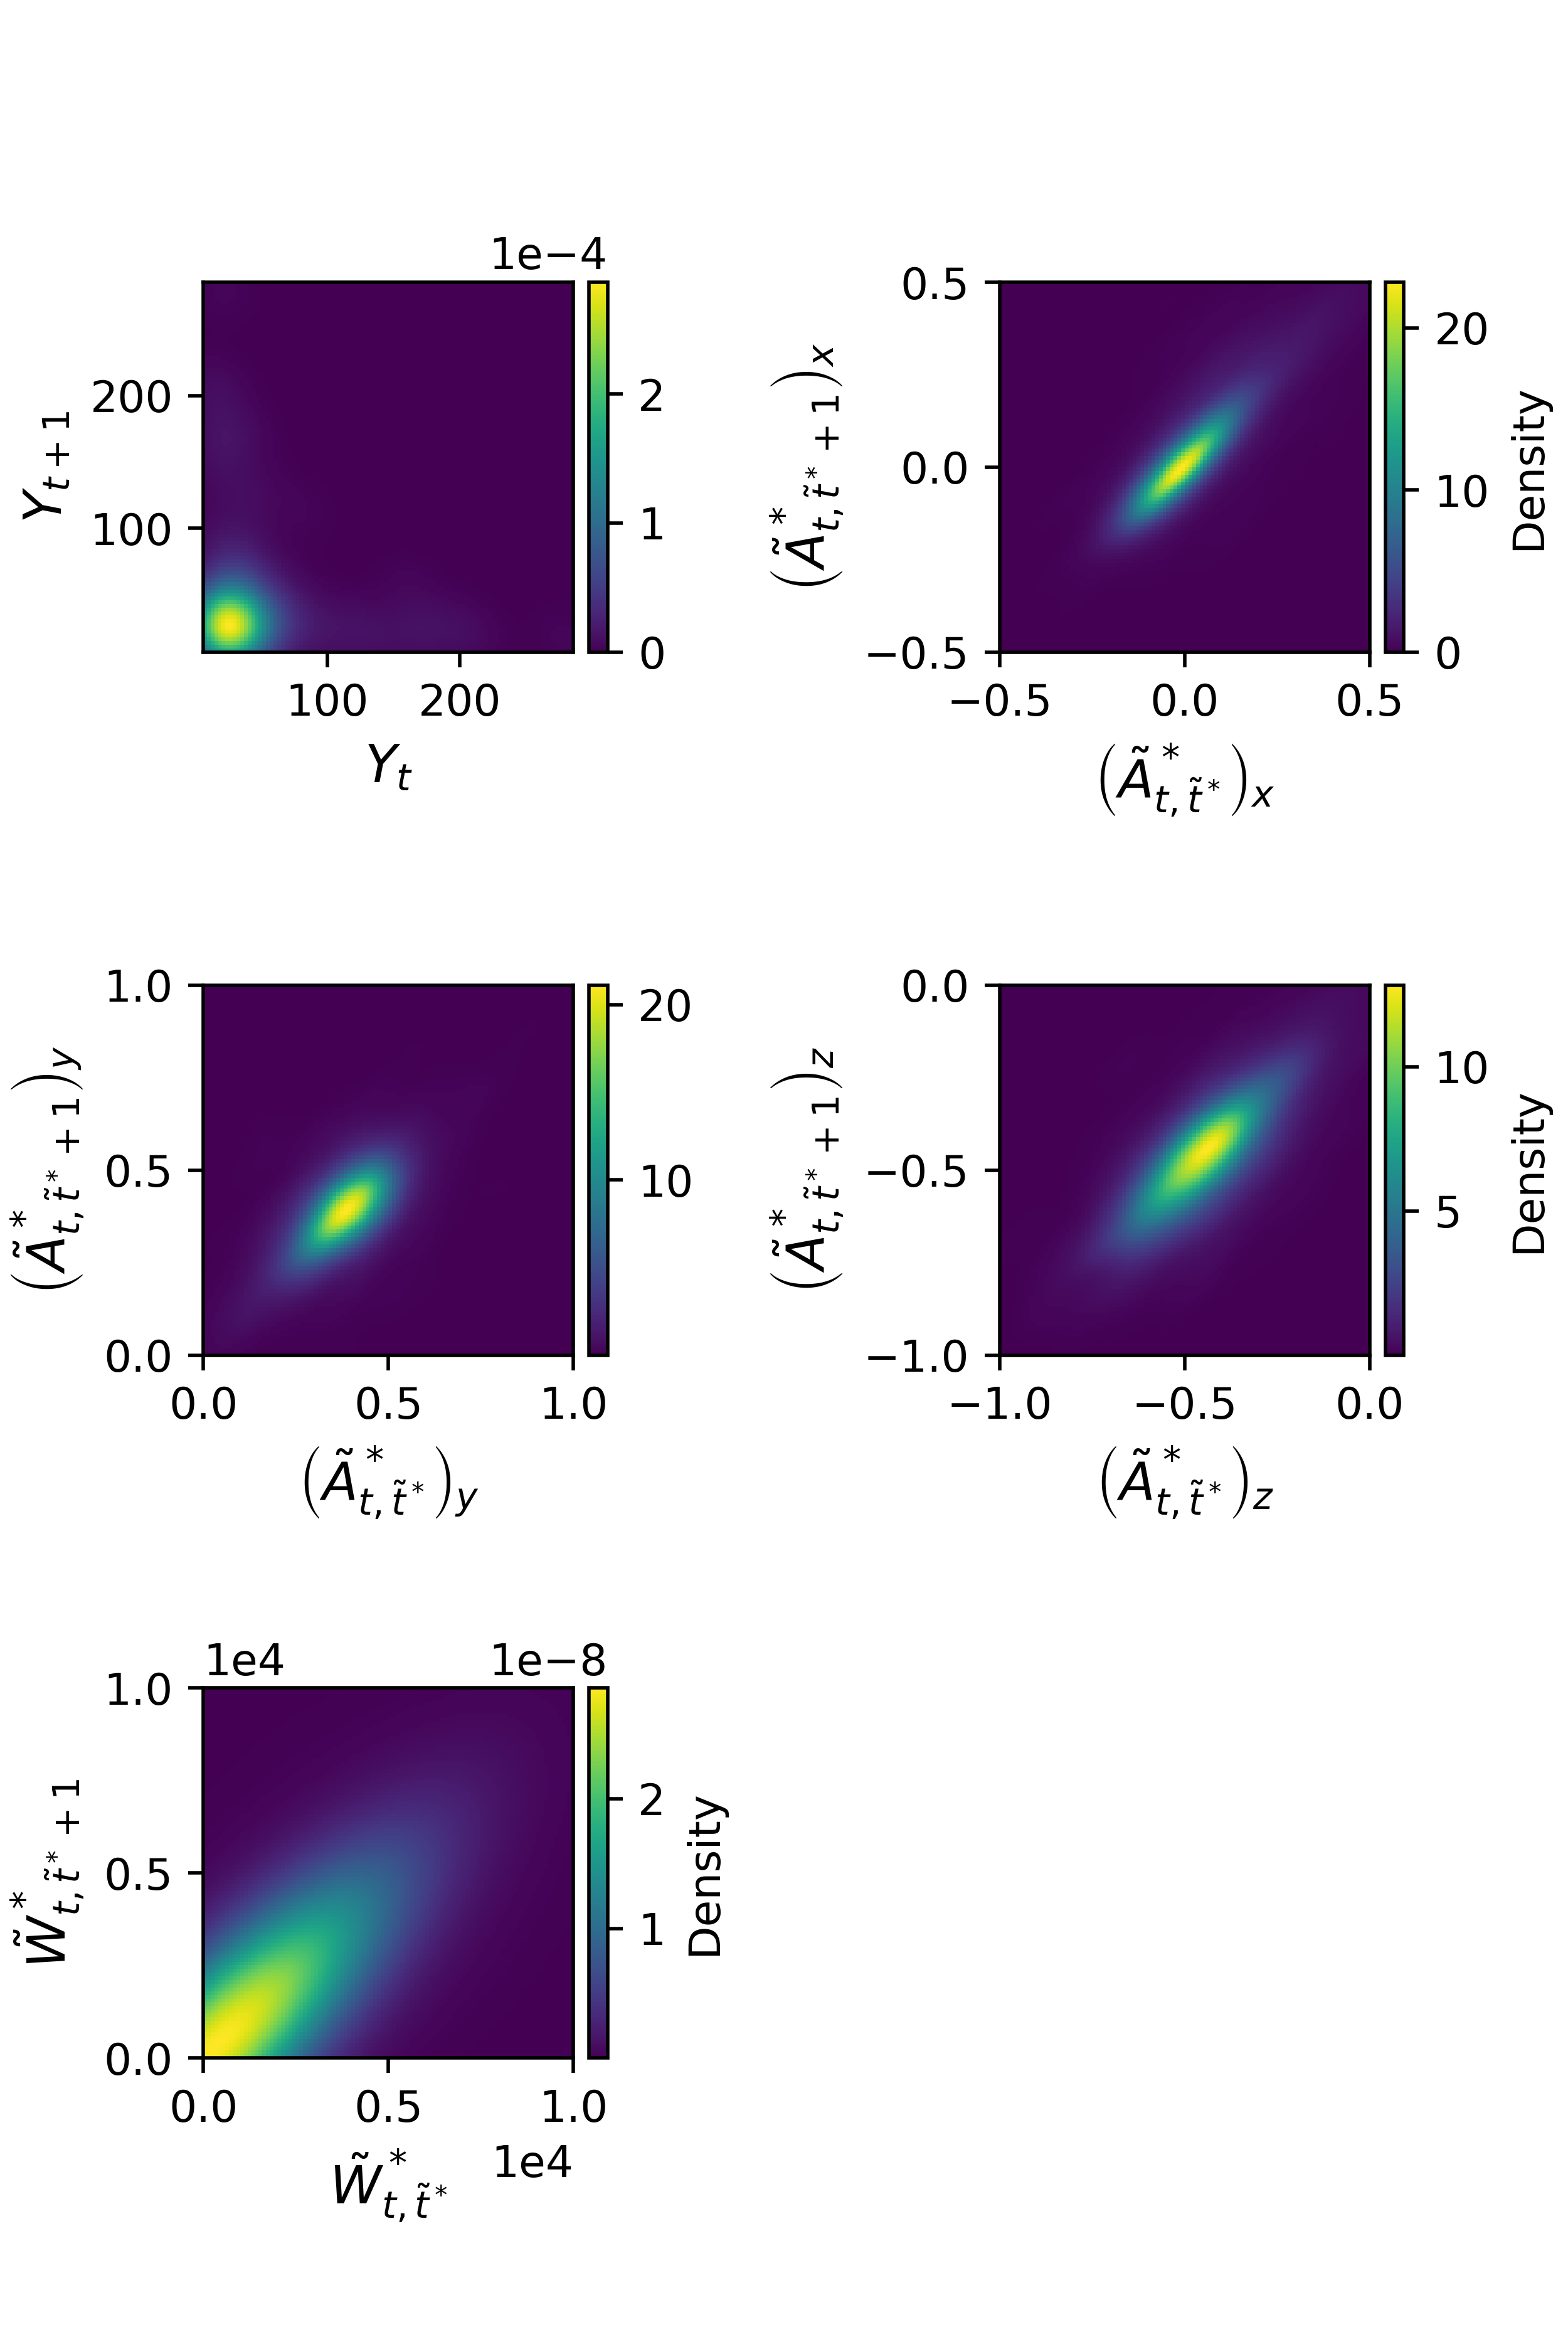
\includegraphics[height=5in]{../Plots/2019/20190902-182840-CATs_OB_1_0_267_CarHHMM2_lagplot.png}
        \end{center}
        
        \noindent Figure \arabic{fignum}: Collection of 5 lag plots where a given observation is on the $x$-axis and the subsequent observation is on the $y$-axis. Each plot corresponds to a feature in the killer whale dive data. Lag plots are used to decide whether to include auto-correlation in the HMMs used to model the killer whale's kinematic data. They can also be used to determine the number of hidden states if multiple distinct patterns are visible. 
        \addtocounter{fignum}{1}
        
        \newpage
        
    \section{Likelihood Surface of the CarHHMM-DFT}
    
        \begin{center}
        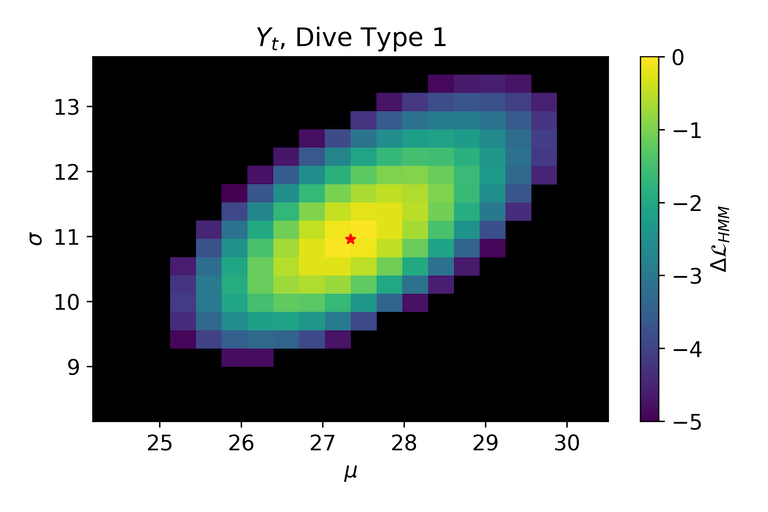
\includegraphics[width=2.25in]{../Plots/2019/20190902-182840-CATs_OB_1_0_267_CarHHMM2_coarse-theta-likelihood-dive_duration-1.png}
        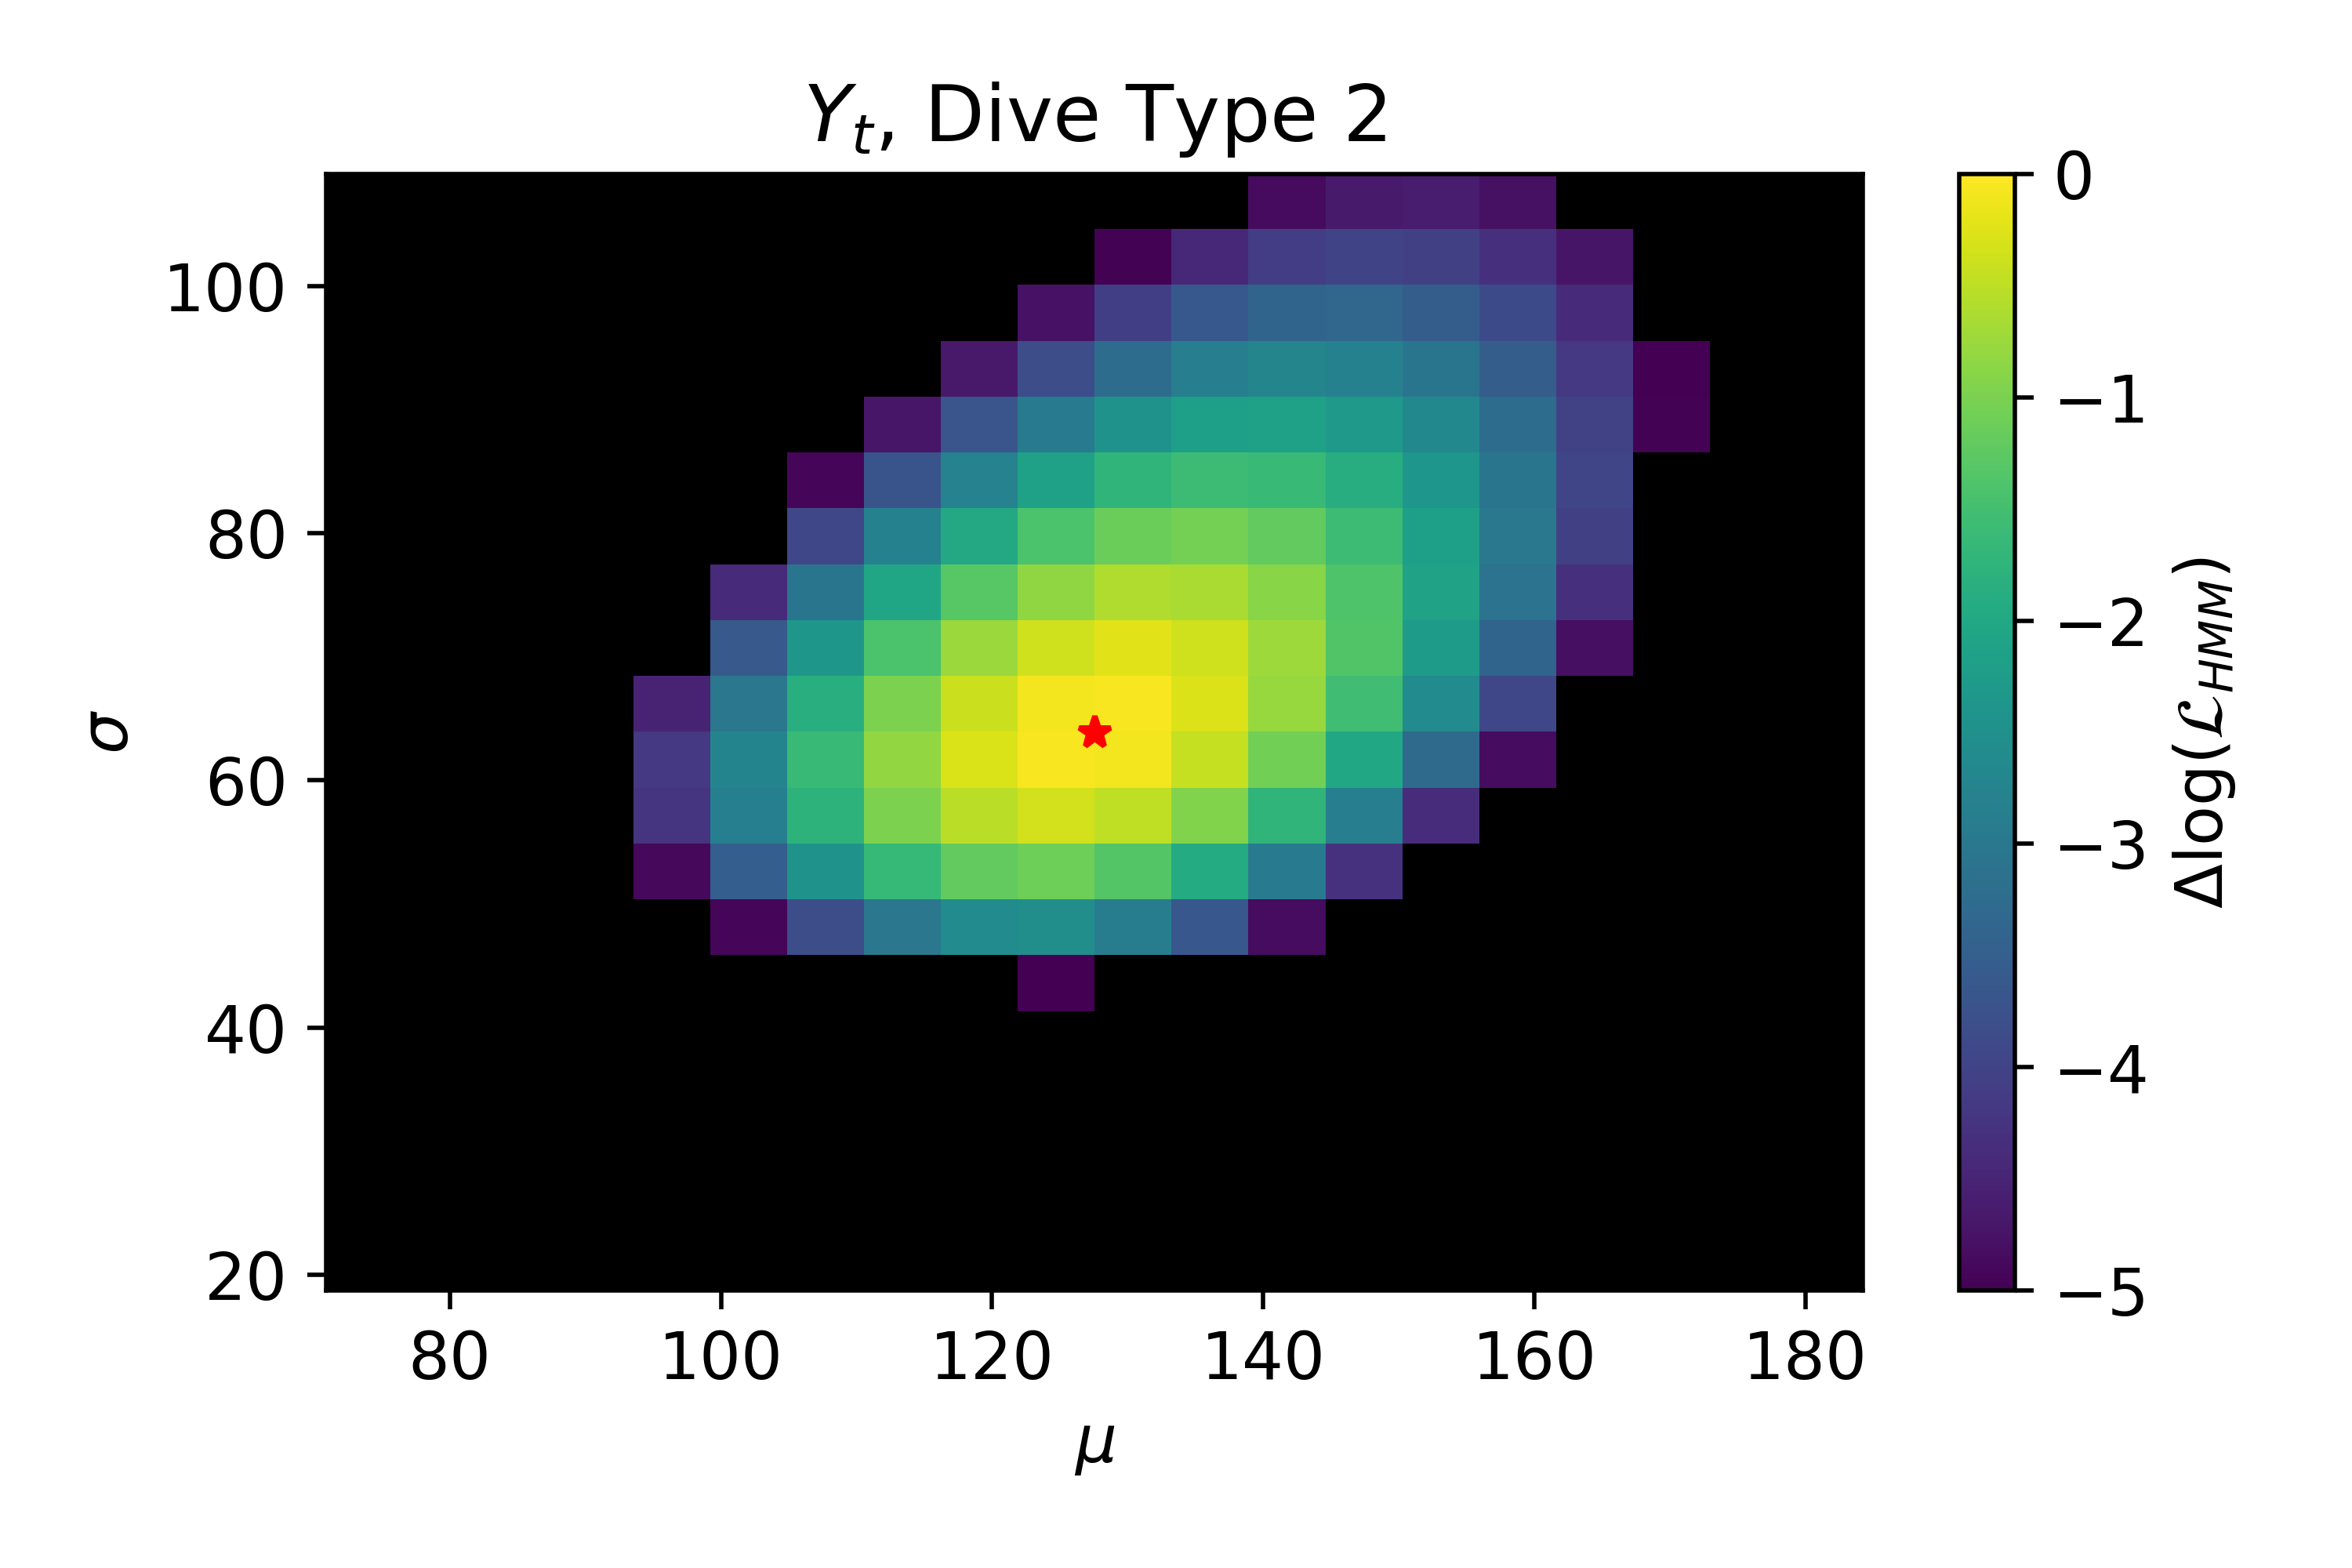
\includegraphics[width=2.25in]{../Plots/2019/20190902-182840-CATs_OB_1_0_267_CarHHMM2_coarse-theta-likelihood-dive_duration-2.png}
        \end{center}
        
        \noindent Figure \arabic{fignum}: Log-likelihood of the CarHHMM-DFT as a function of the dive duration parameters $\mu_Y^{(i)}$ and $\sigma_Y^{(i)}$ for dive types $i = 1,2$. All other parameters and probability transition matrices are set to be equal to the maximum likelihood estimates shown in Table (1) of Section 3.1. The log-likelihood is added to the negative log-likelihood of the maximum likelihood estimate $(\hat \mu_Y,\hat \sigma_Y)$, which is denoted by a red star.
        \addtocounter{fignum}{1}
        
        
        \begin{center}
        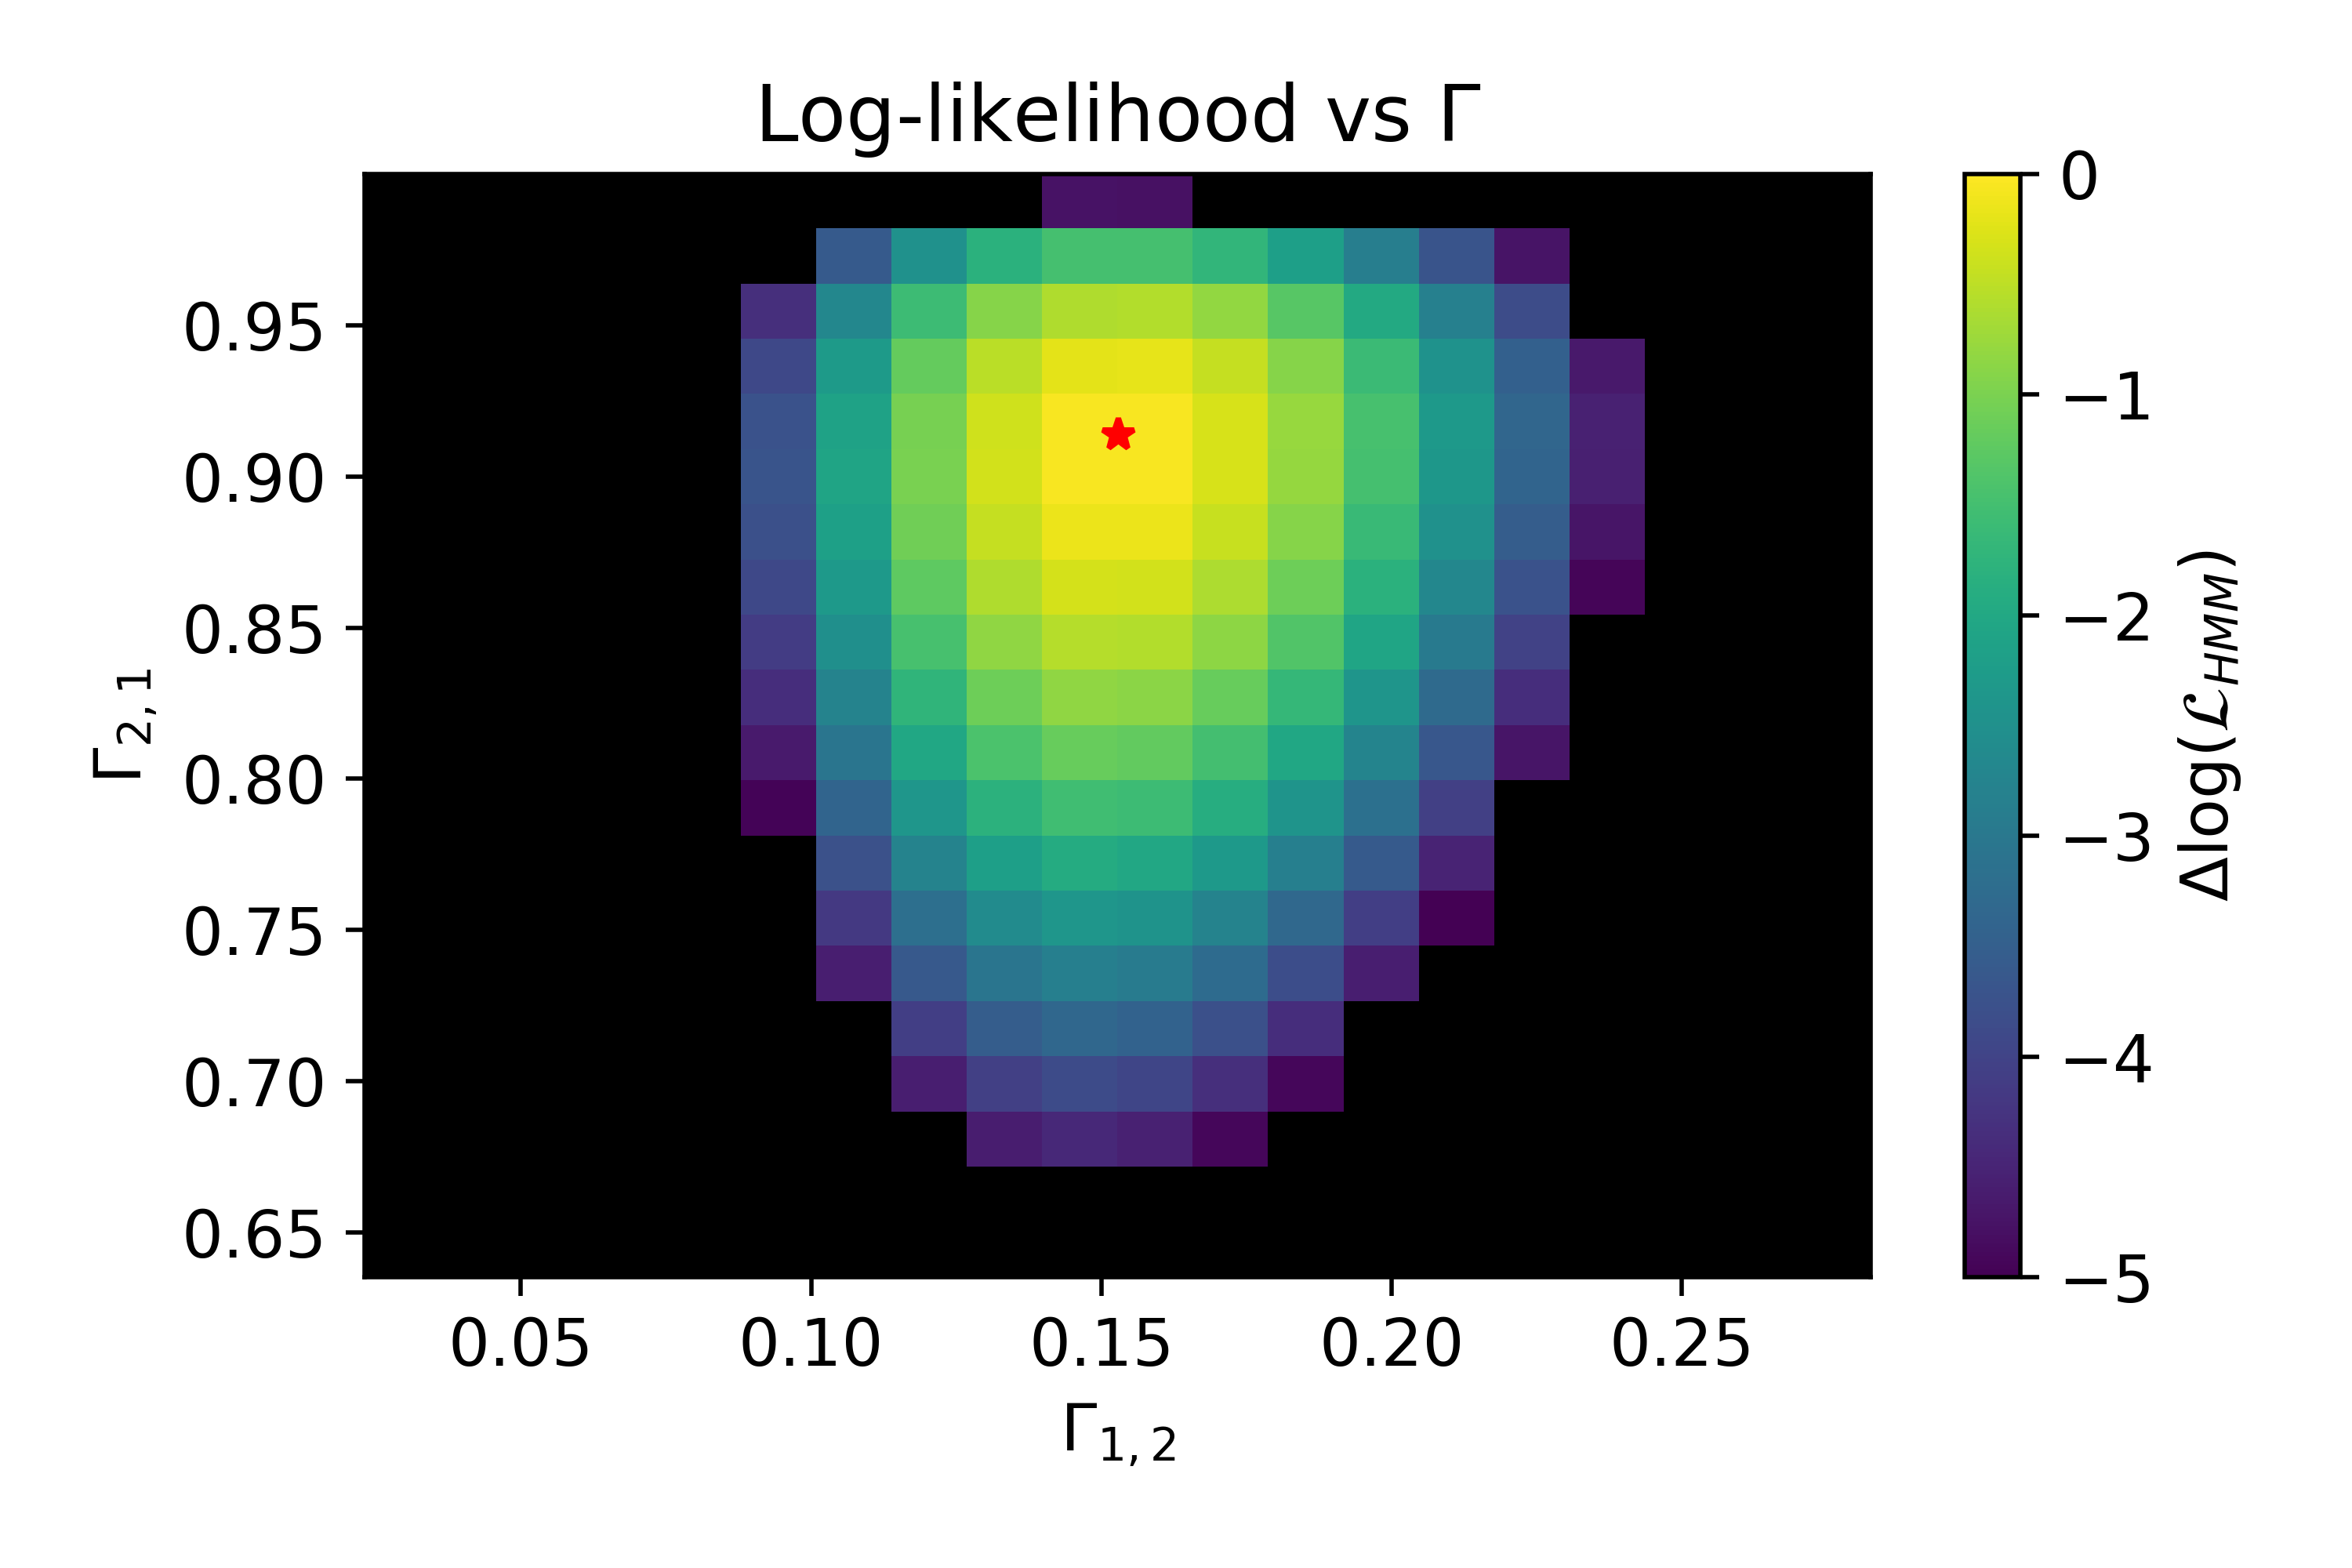
\includegraphics[width=2.1in]{../Plots/2019/20190902-182840-CATs_OB_1_0_267_CarHHMM2_coarse-gamma-likelihood.png}
        \end{center}
        
        \noindent Figure \arabic{fignum}: Log-likelihood of the CarHHMM-DFT as a function of the coarse-scale probability transition matrix parameters $\Gamma_{1,2}$ and $\Gamma_{2,1}$. All other parameters and probability transition matrices are set to be equal to the maximum likelihood estimates shown in Table (1) of Section 3.1. The log-likelihood is added to the negative log-likelihood of the maximum likelihood estimate $(\hat \Gamma_{1,2},\hat \Gamma_{2,1})$, which is denoted by a red star.
        \addtocounter{fignum}{1}
        
        % Ahat_low
        \begin{center}
        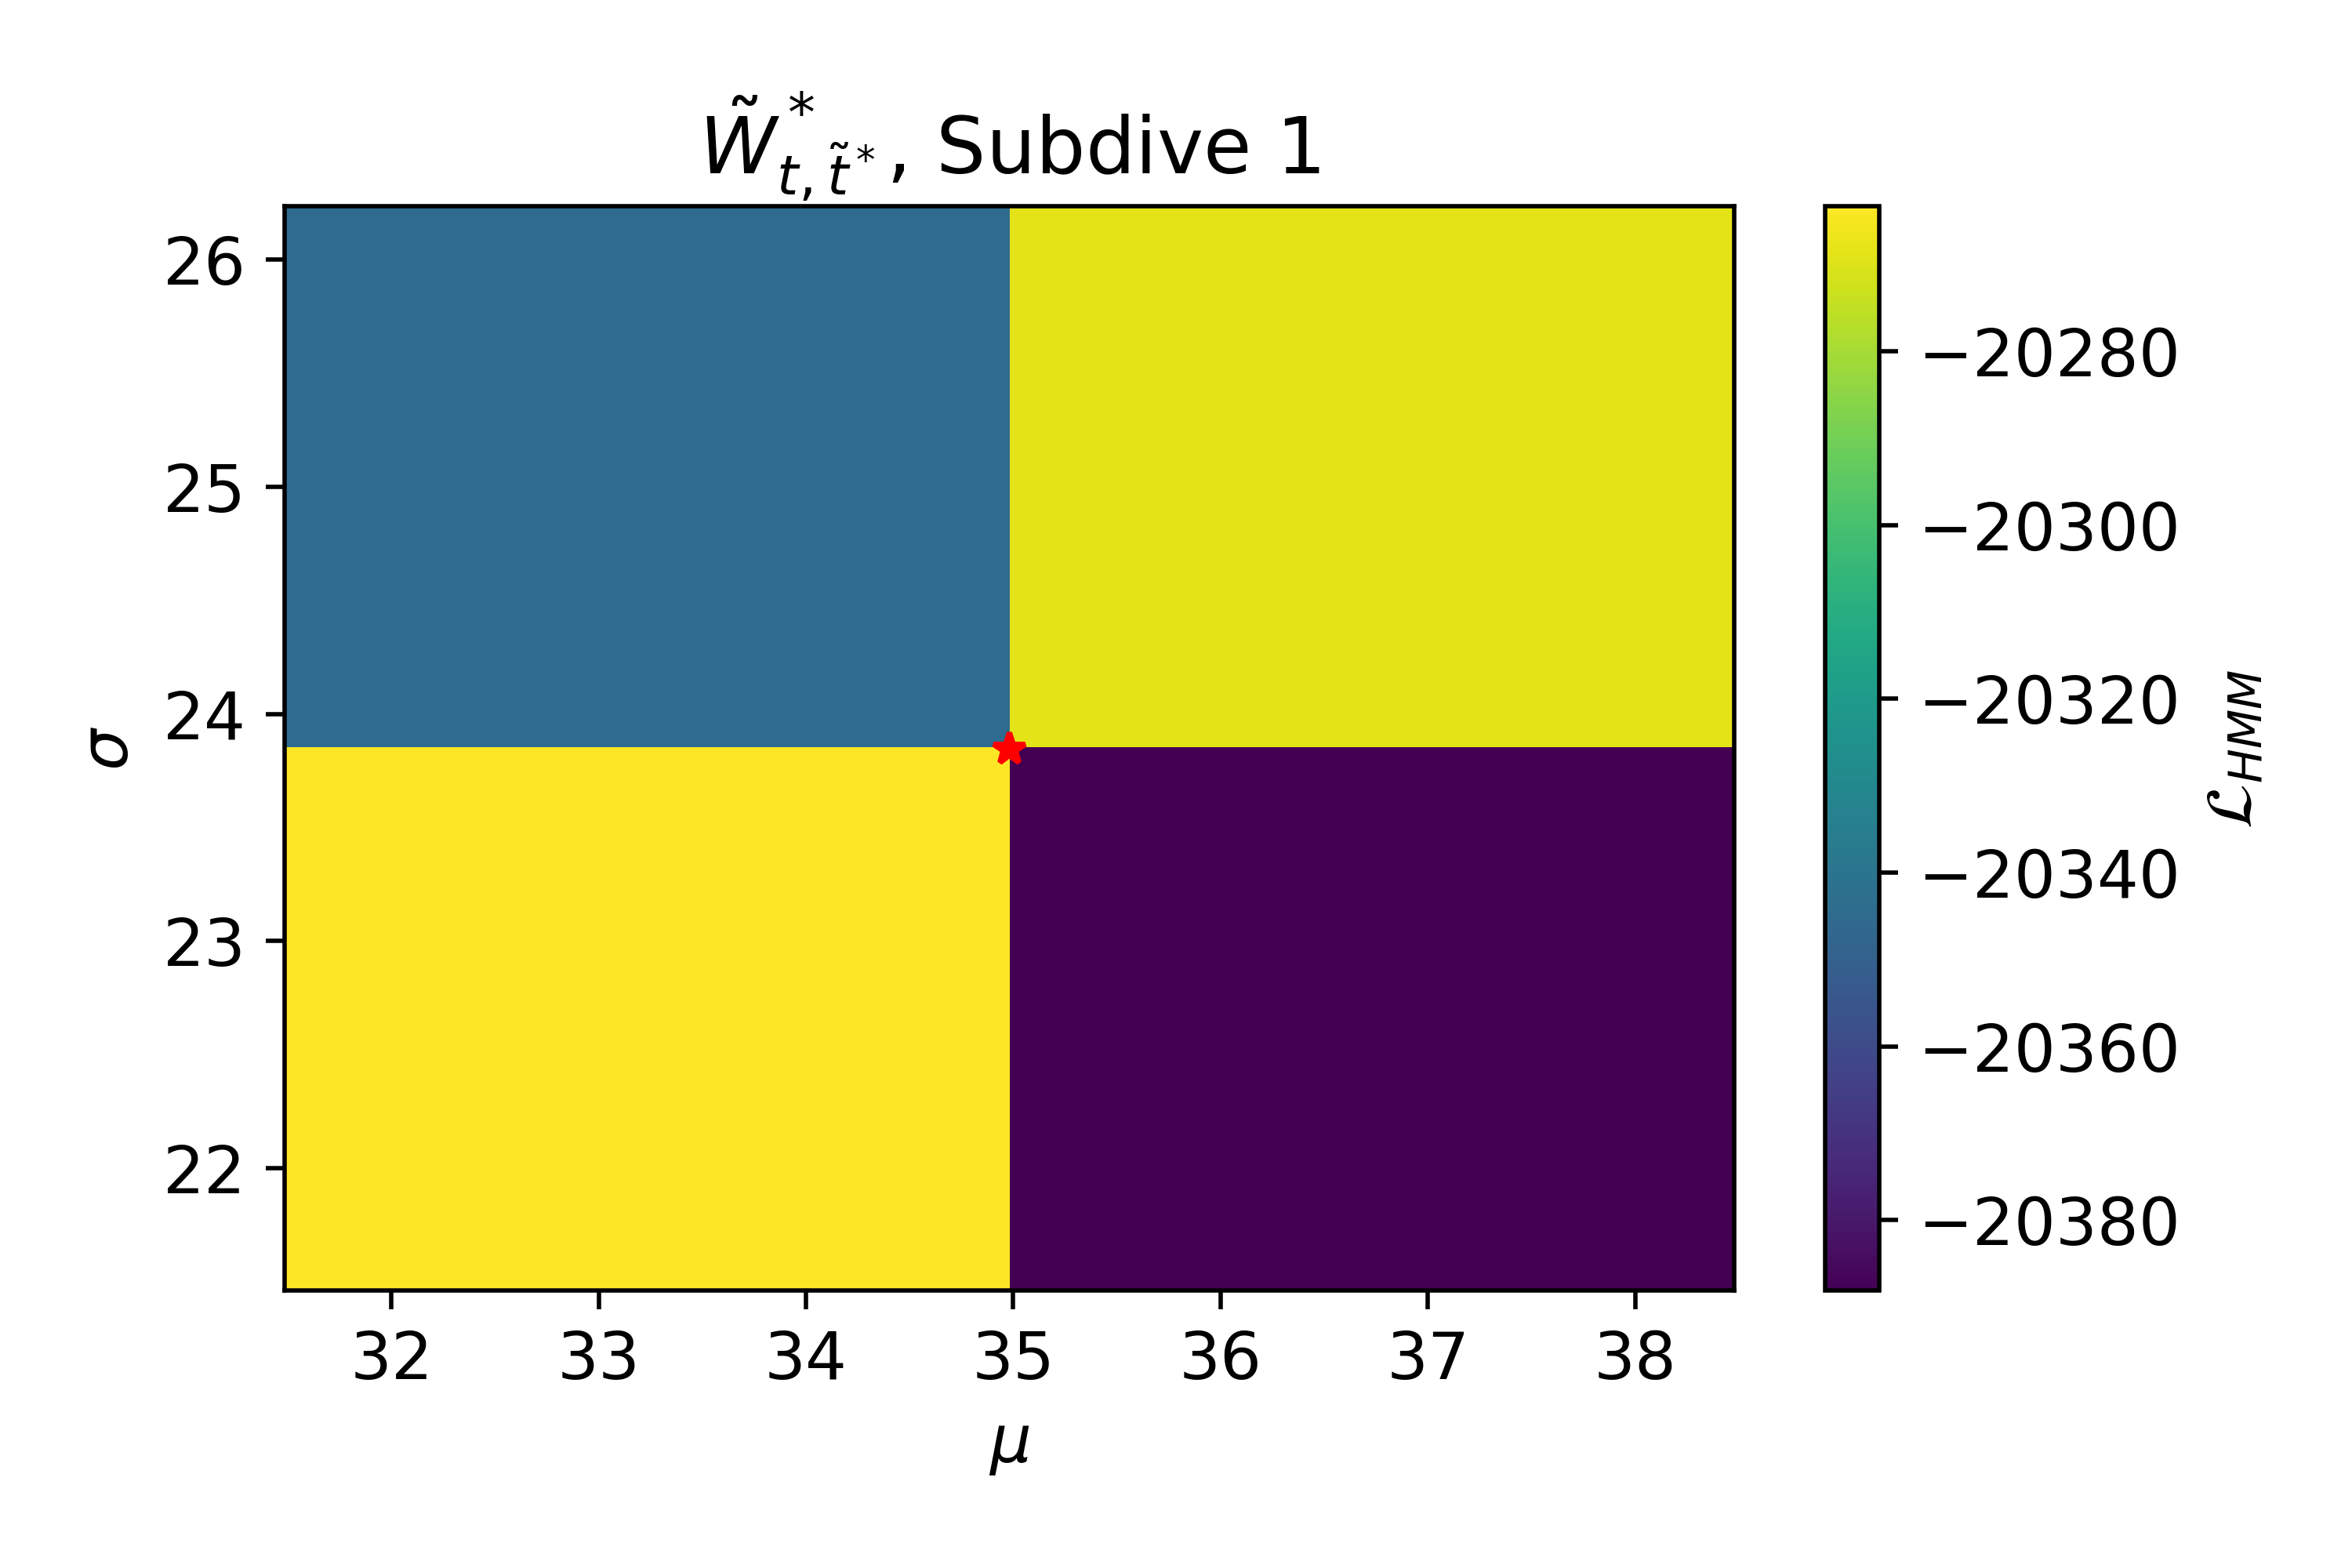
\includegraphics[width=2.1in]{../Plots/2019/20190902-182840-CATs_OB_1_0_267_CarHHMM2_fine-theta-likelihood-Ahat_low-0.png}
        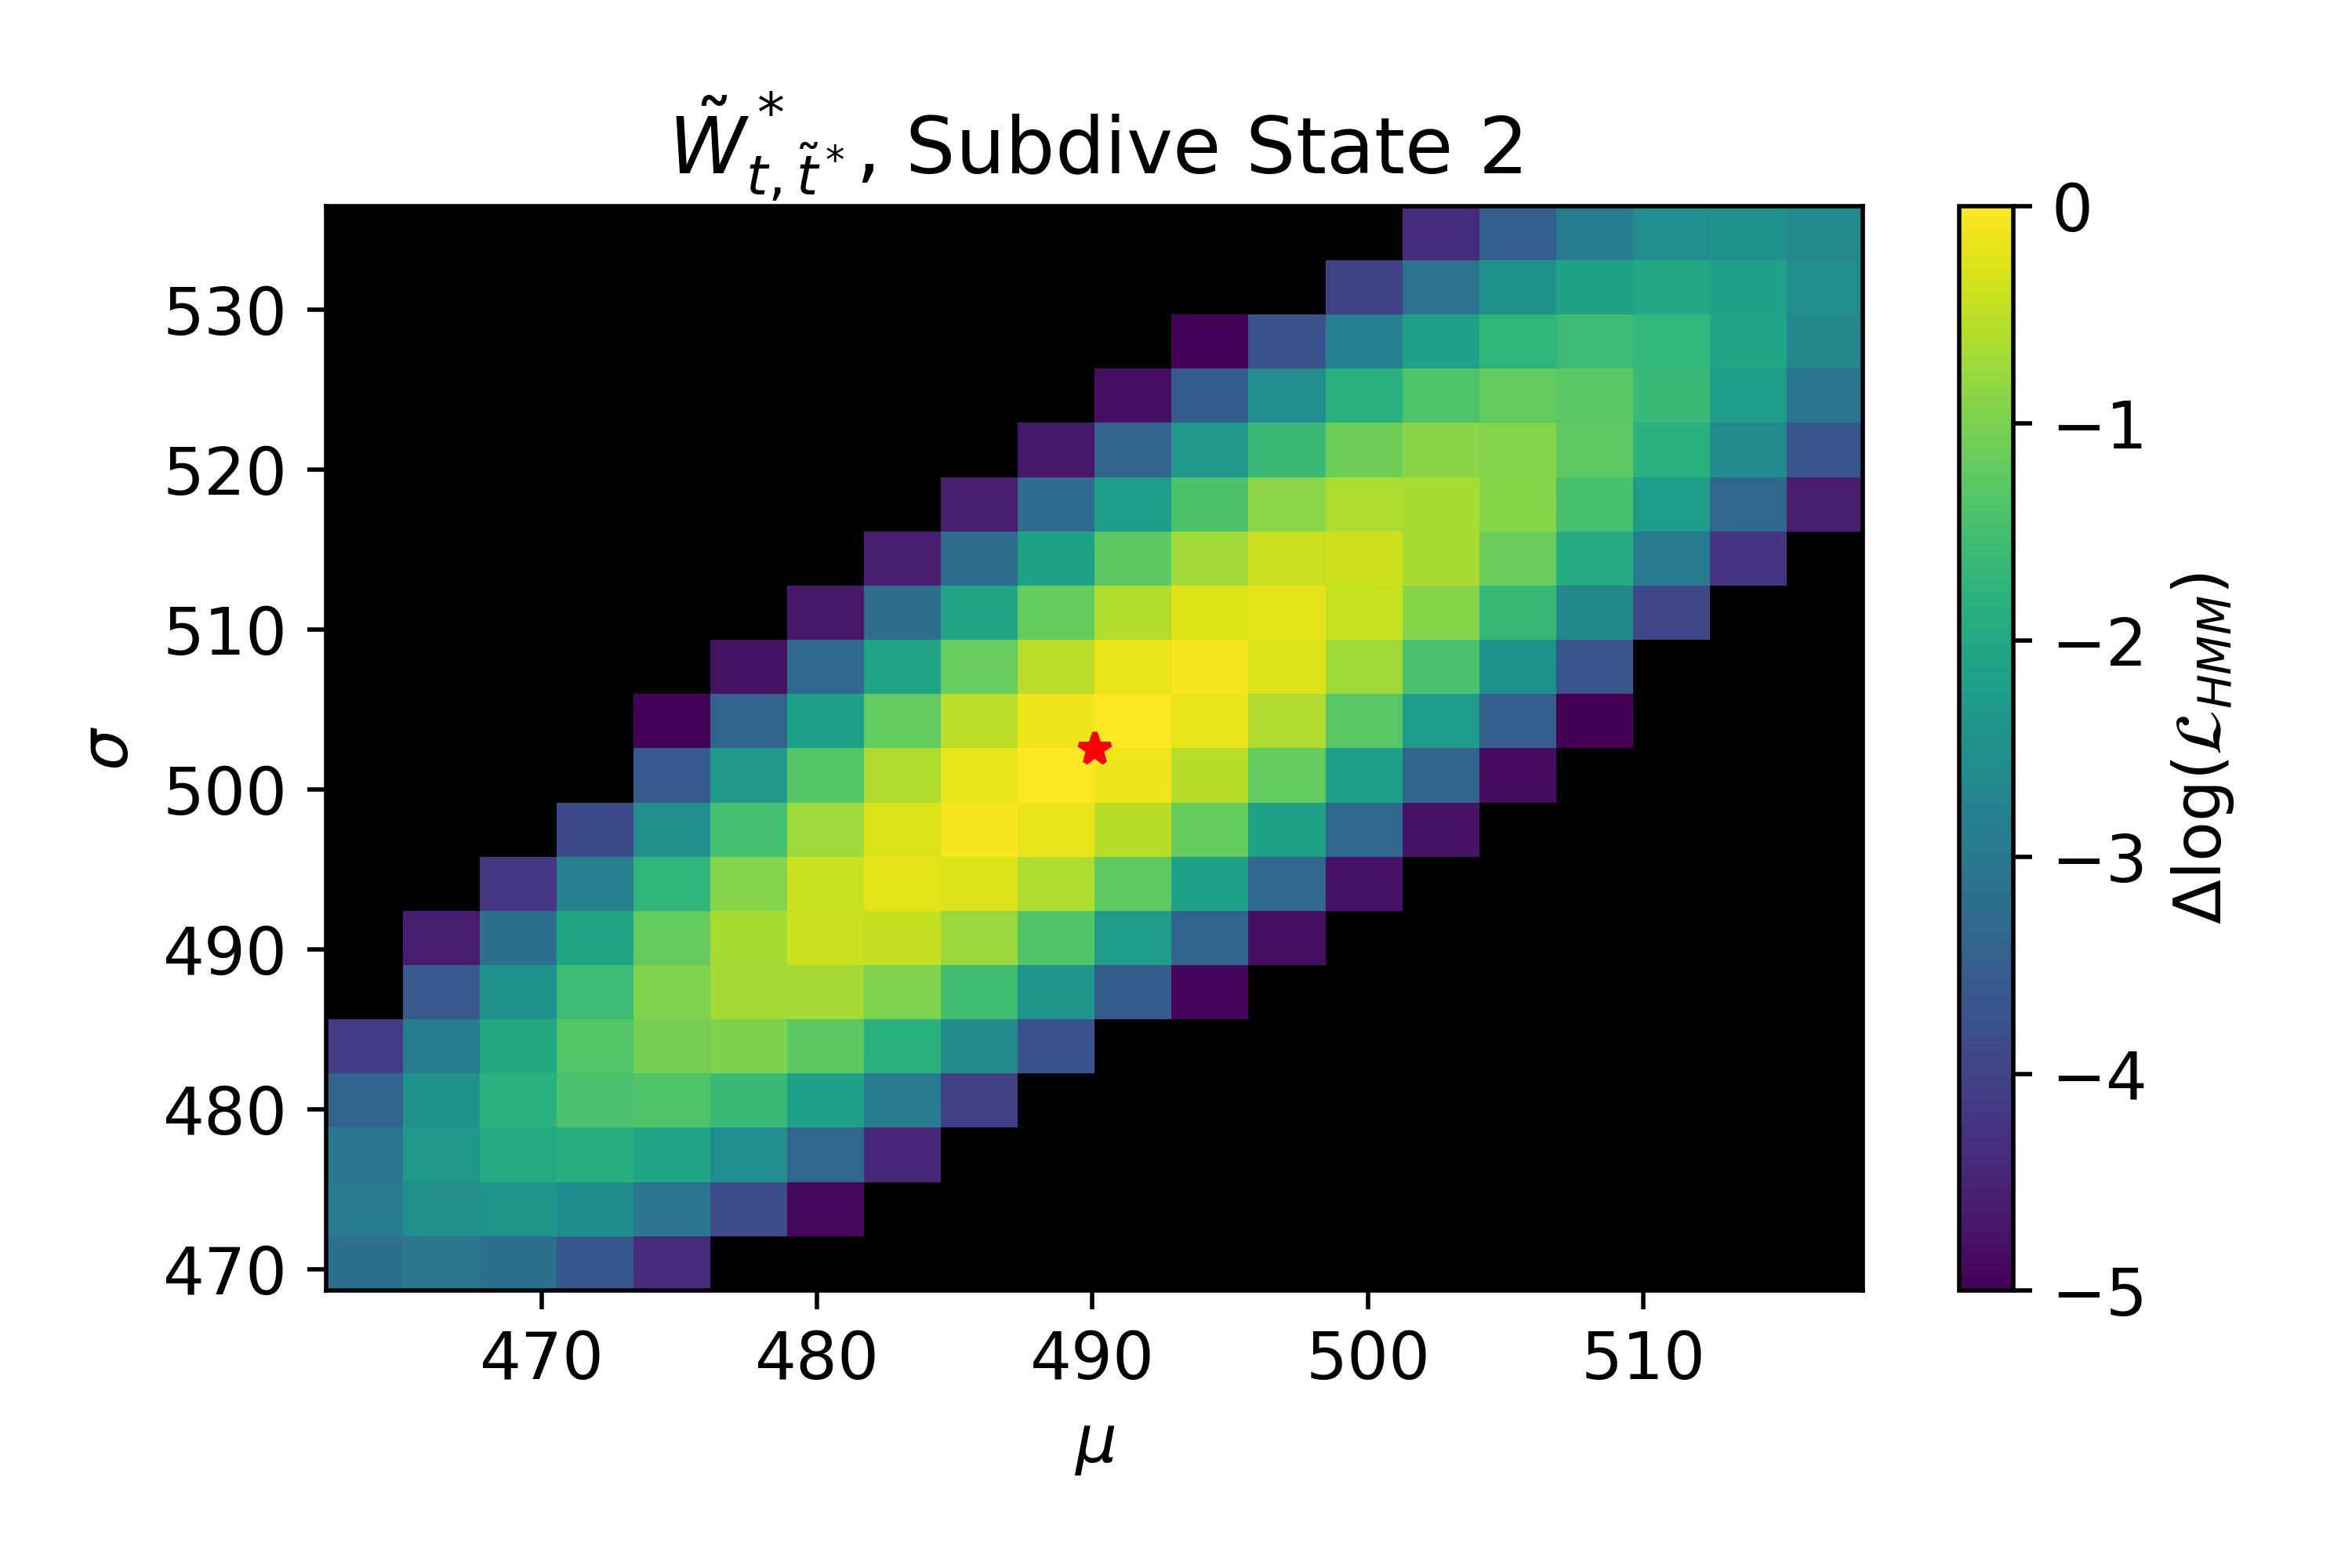
\includegraphics[width=2.1in]{../Plots/2019/20190902-182840-CATs_OB_1_0_267_CarHHMM2_fine-theta-likelihood-Ahat_low-1.png}
        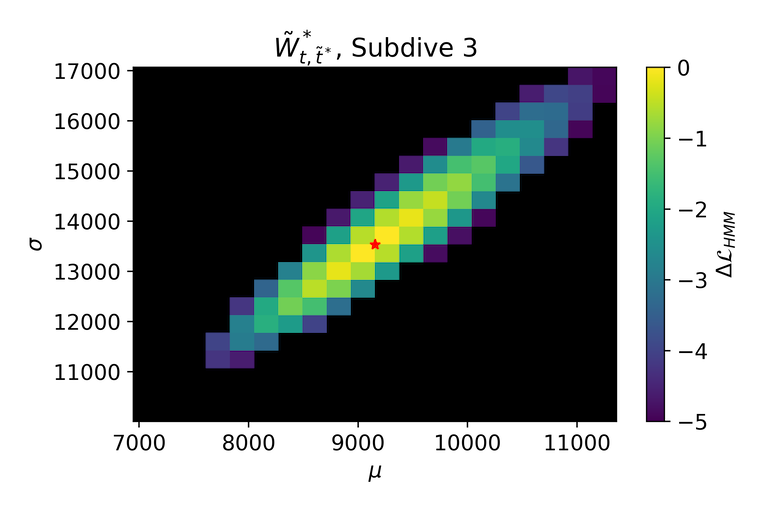
\includegraphics[width=2.1in]{../Plots/2019/20190902-182840-CATs_OB_1_0_267_CarHHMM2_fine-theta-likelihood-Ahat_low-2.png}
        \end{center}
        
        \noindent Figure \arabic{fignum}: Log-likelihood of the CarHHMM-DFT as a function of the wiggliness parameters $\mu_W^{*(\cdot,i^*)}$ and $\sigma_W^{*(\cdot,i^*)}$ for subdive types $i^* = 1,2,3$. All other parameters and probability transition matrices are set to be equal to the maximum likelihood estimates shown in Table (1) of Section 3.1. The log-likelihood is added to the negative log-likelihood of the maximum likelihood estimate $(\hat \mu_W^{*(\cdot,i^*)}, \hat \sigma_W^{*(\cdot,i^*)})$, which is denoted by a red star.
        \addtocounter{fignum}{1}
        
        \newpage
        
        % Ax
        \begin{center}
        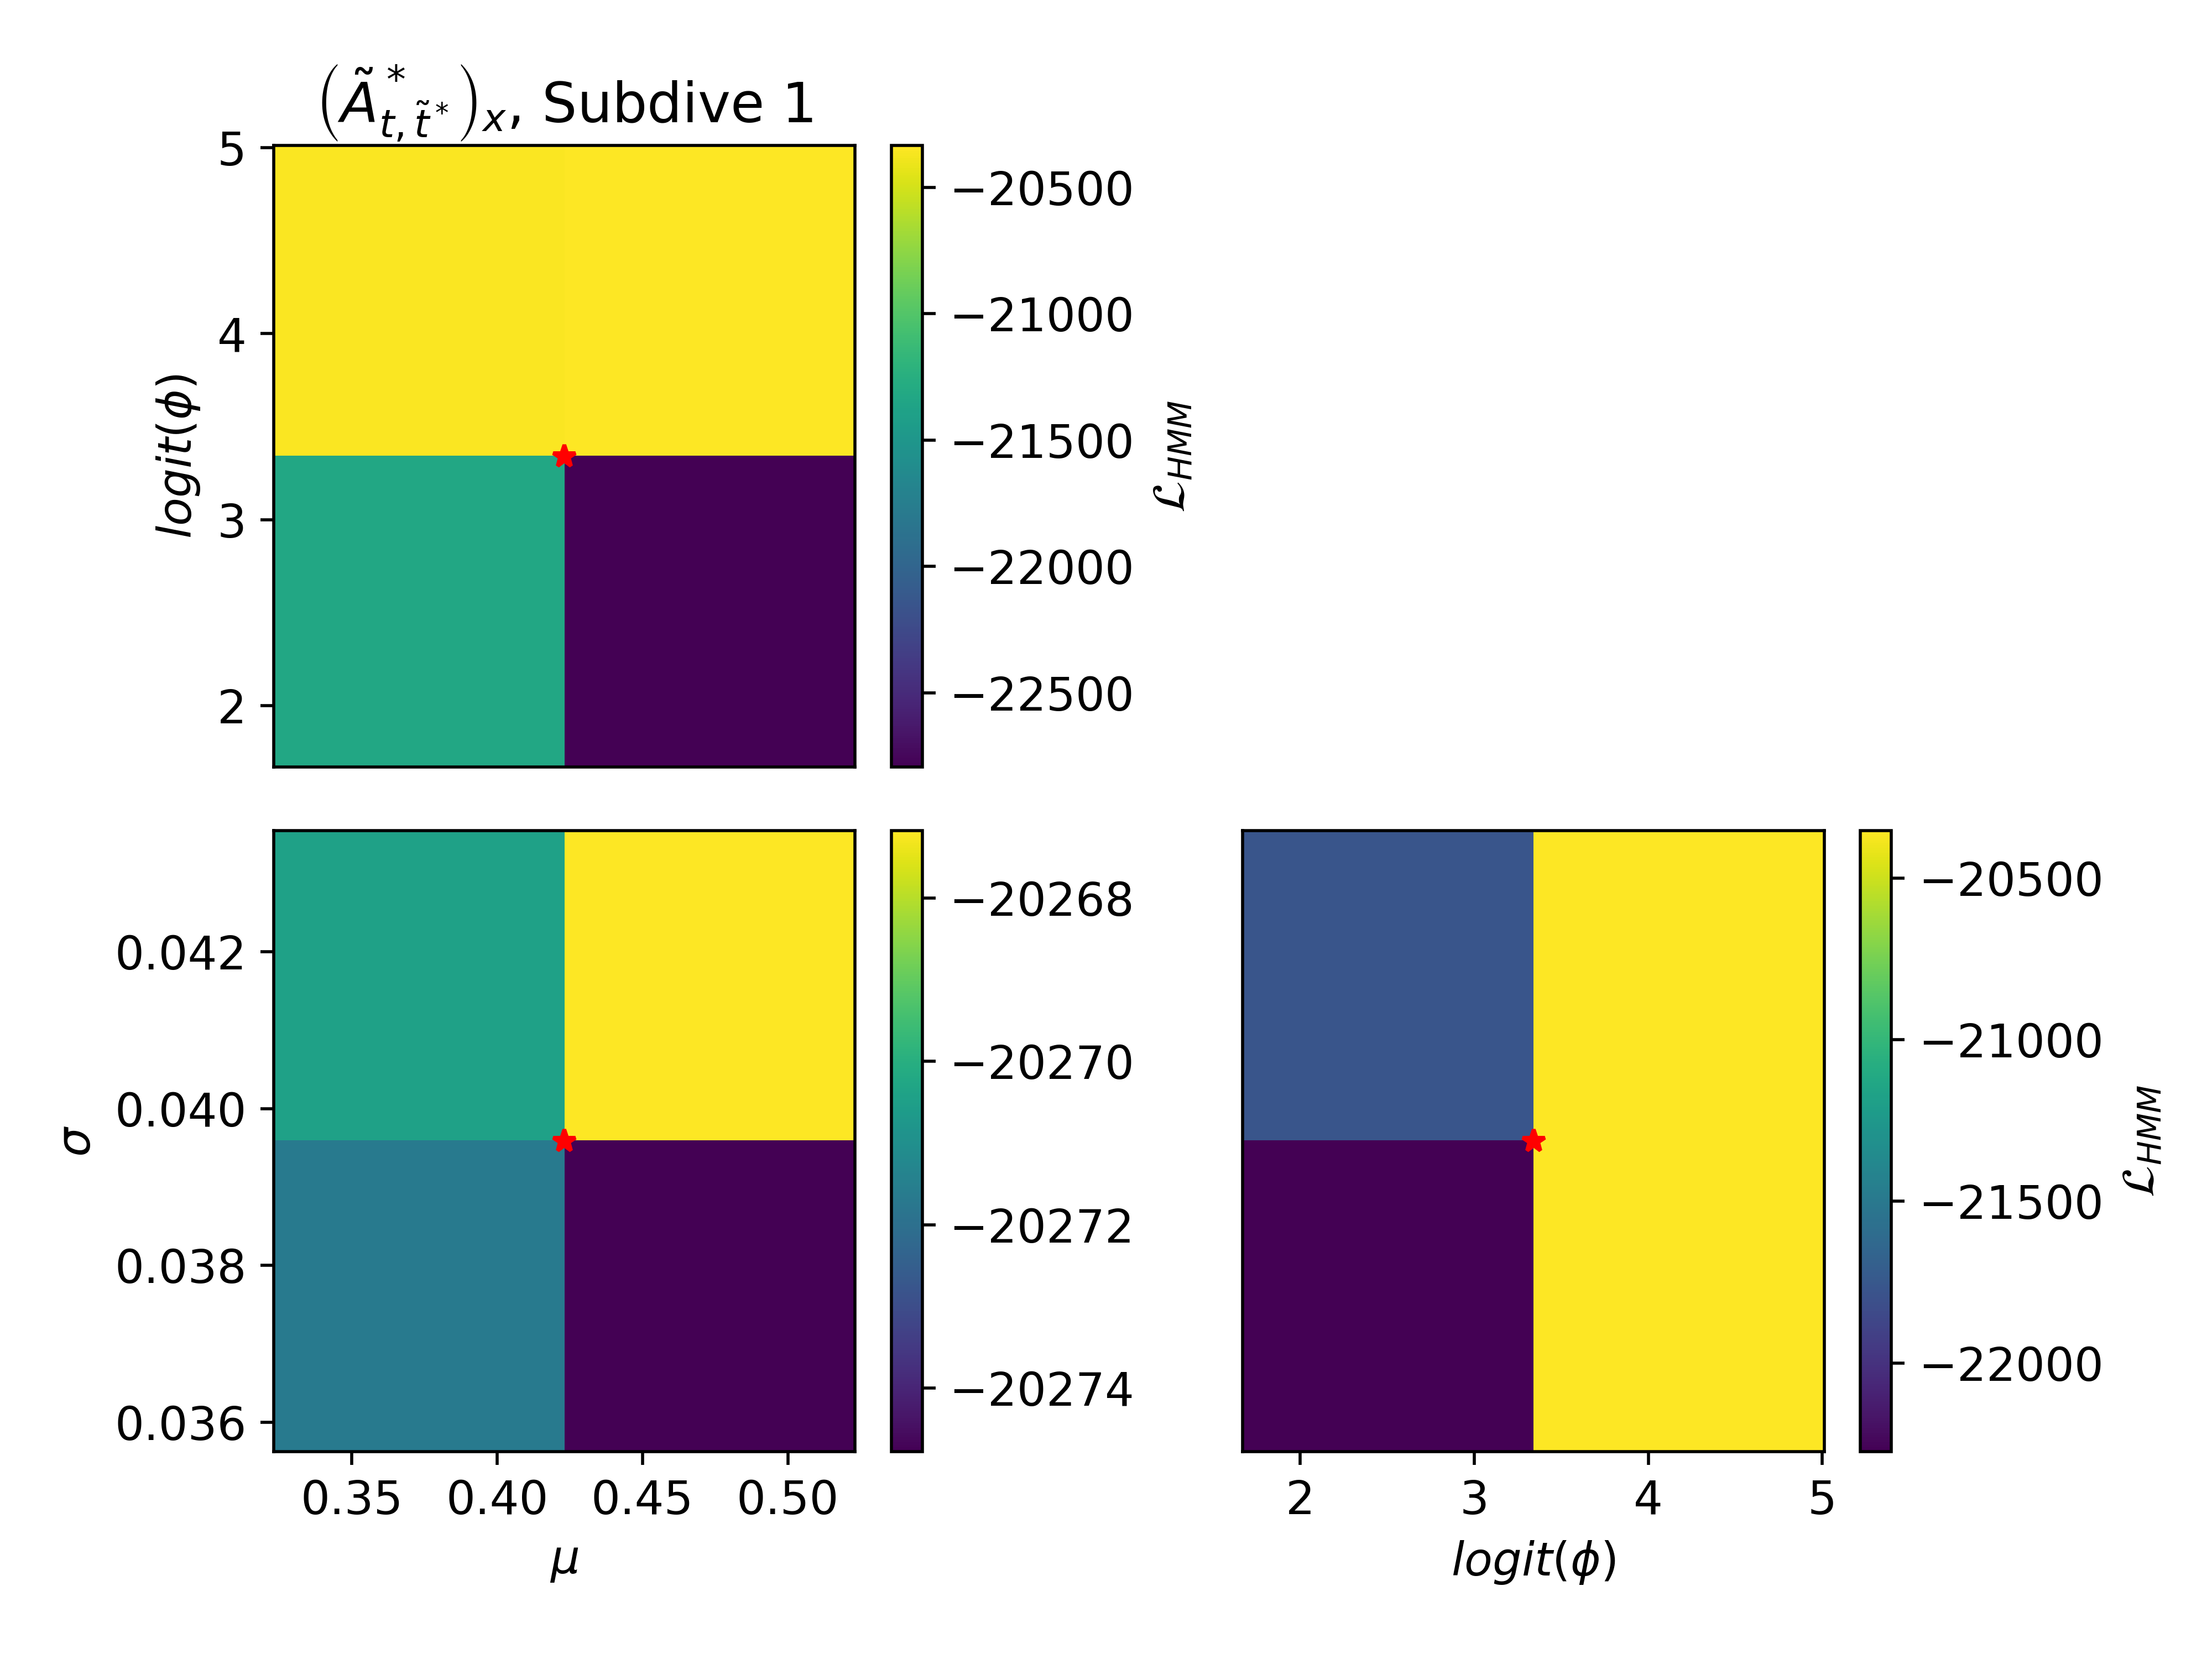
\includegraphics[width=2.1in]{../Plots/2019/20190902-182840-CATs_OB_1_0_267_CarHHMM2_fine-theta-likelihood-Ax-0.png}
        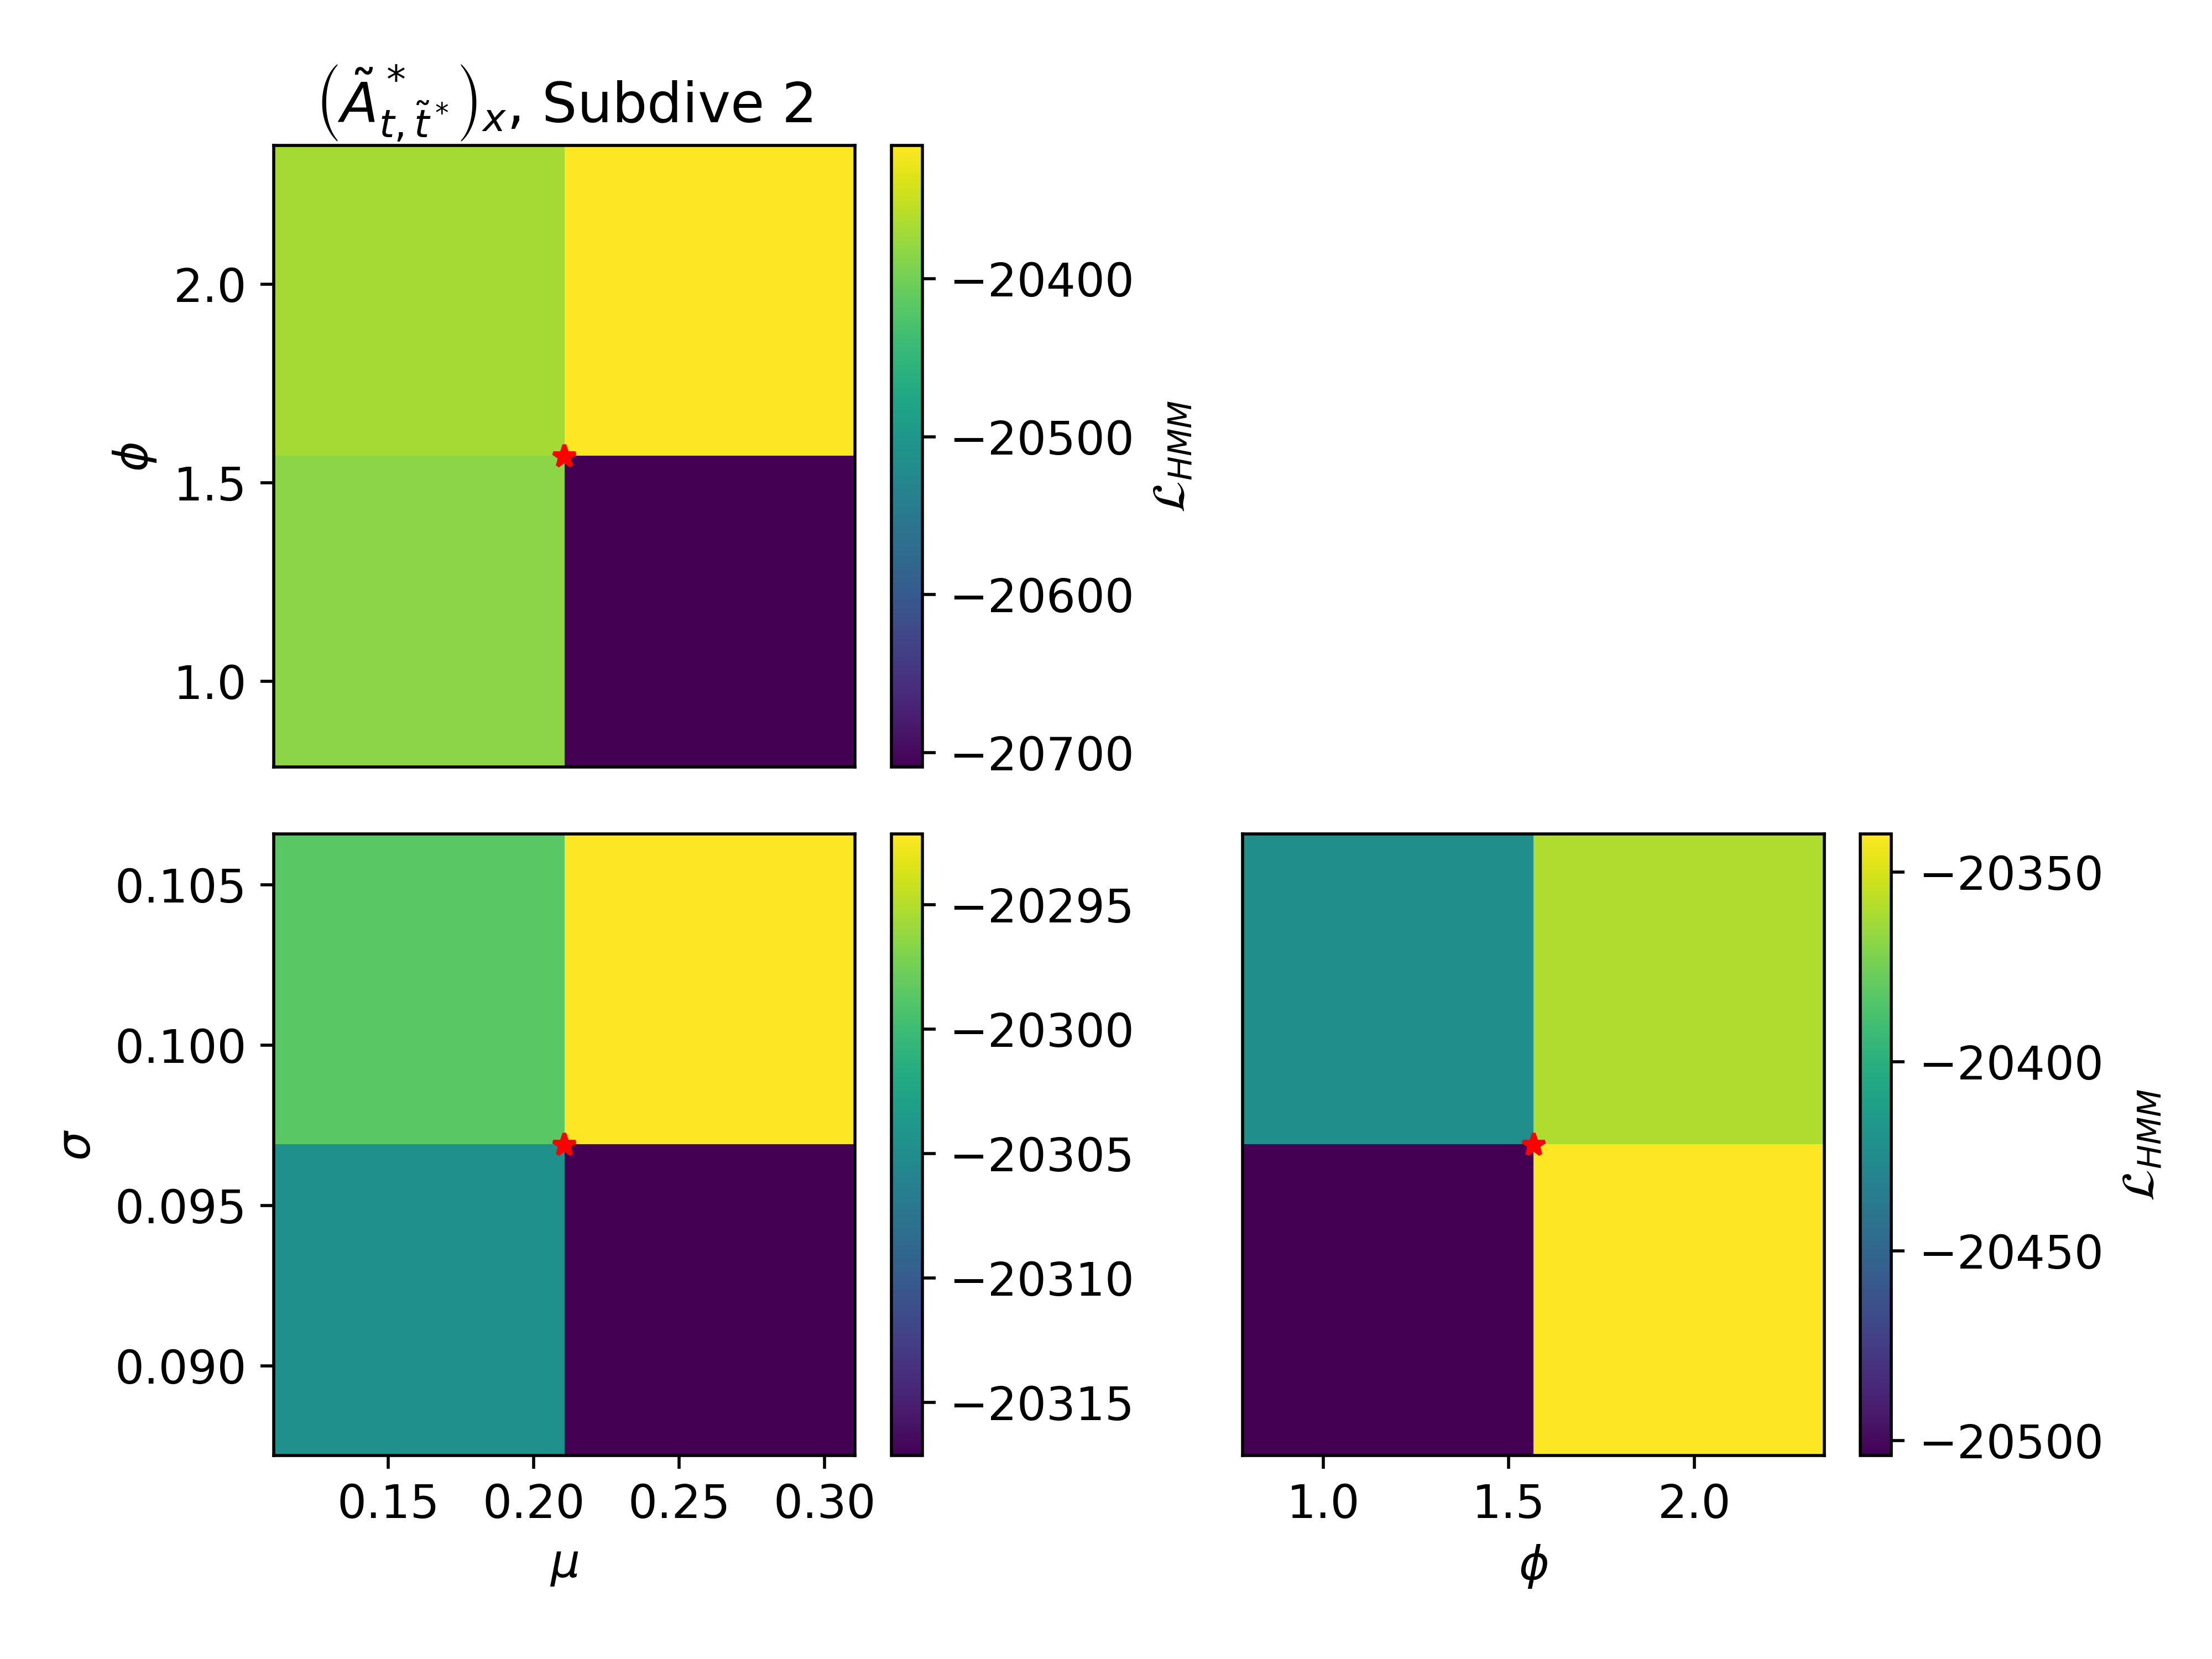
\includegraphics[width=2.1in]{../Plots/2019/20190902-182840-CATs_OB_1_0_267_CarHHMM2_fine-theta-likelihood-Ax-1.png}
        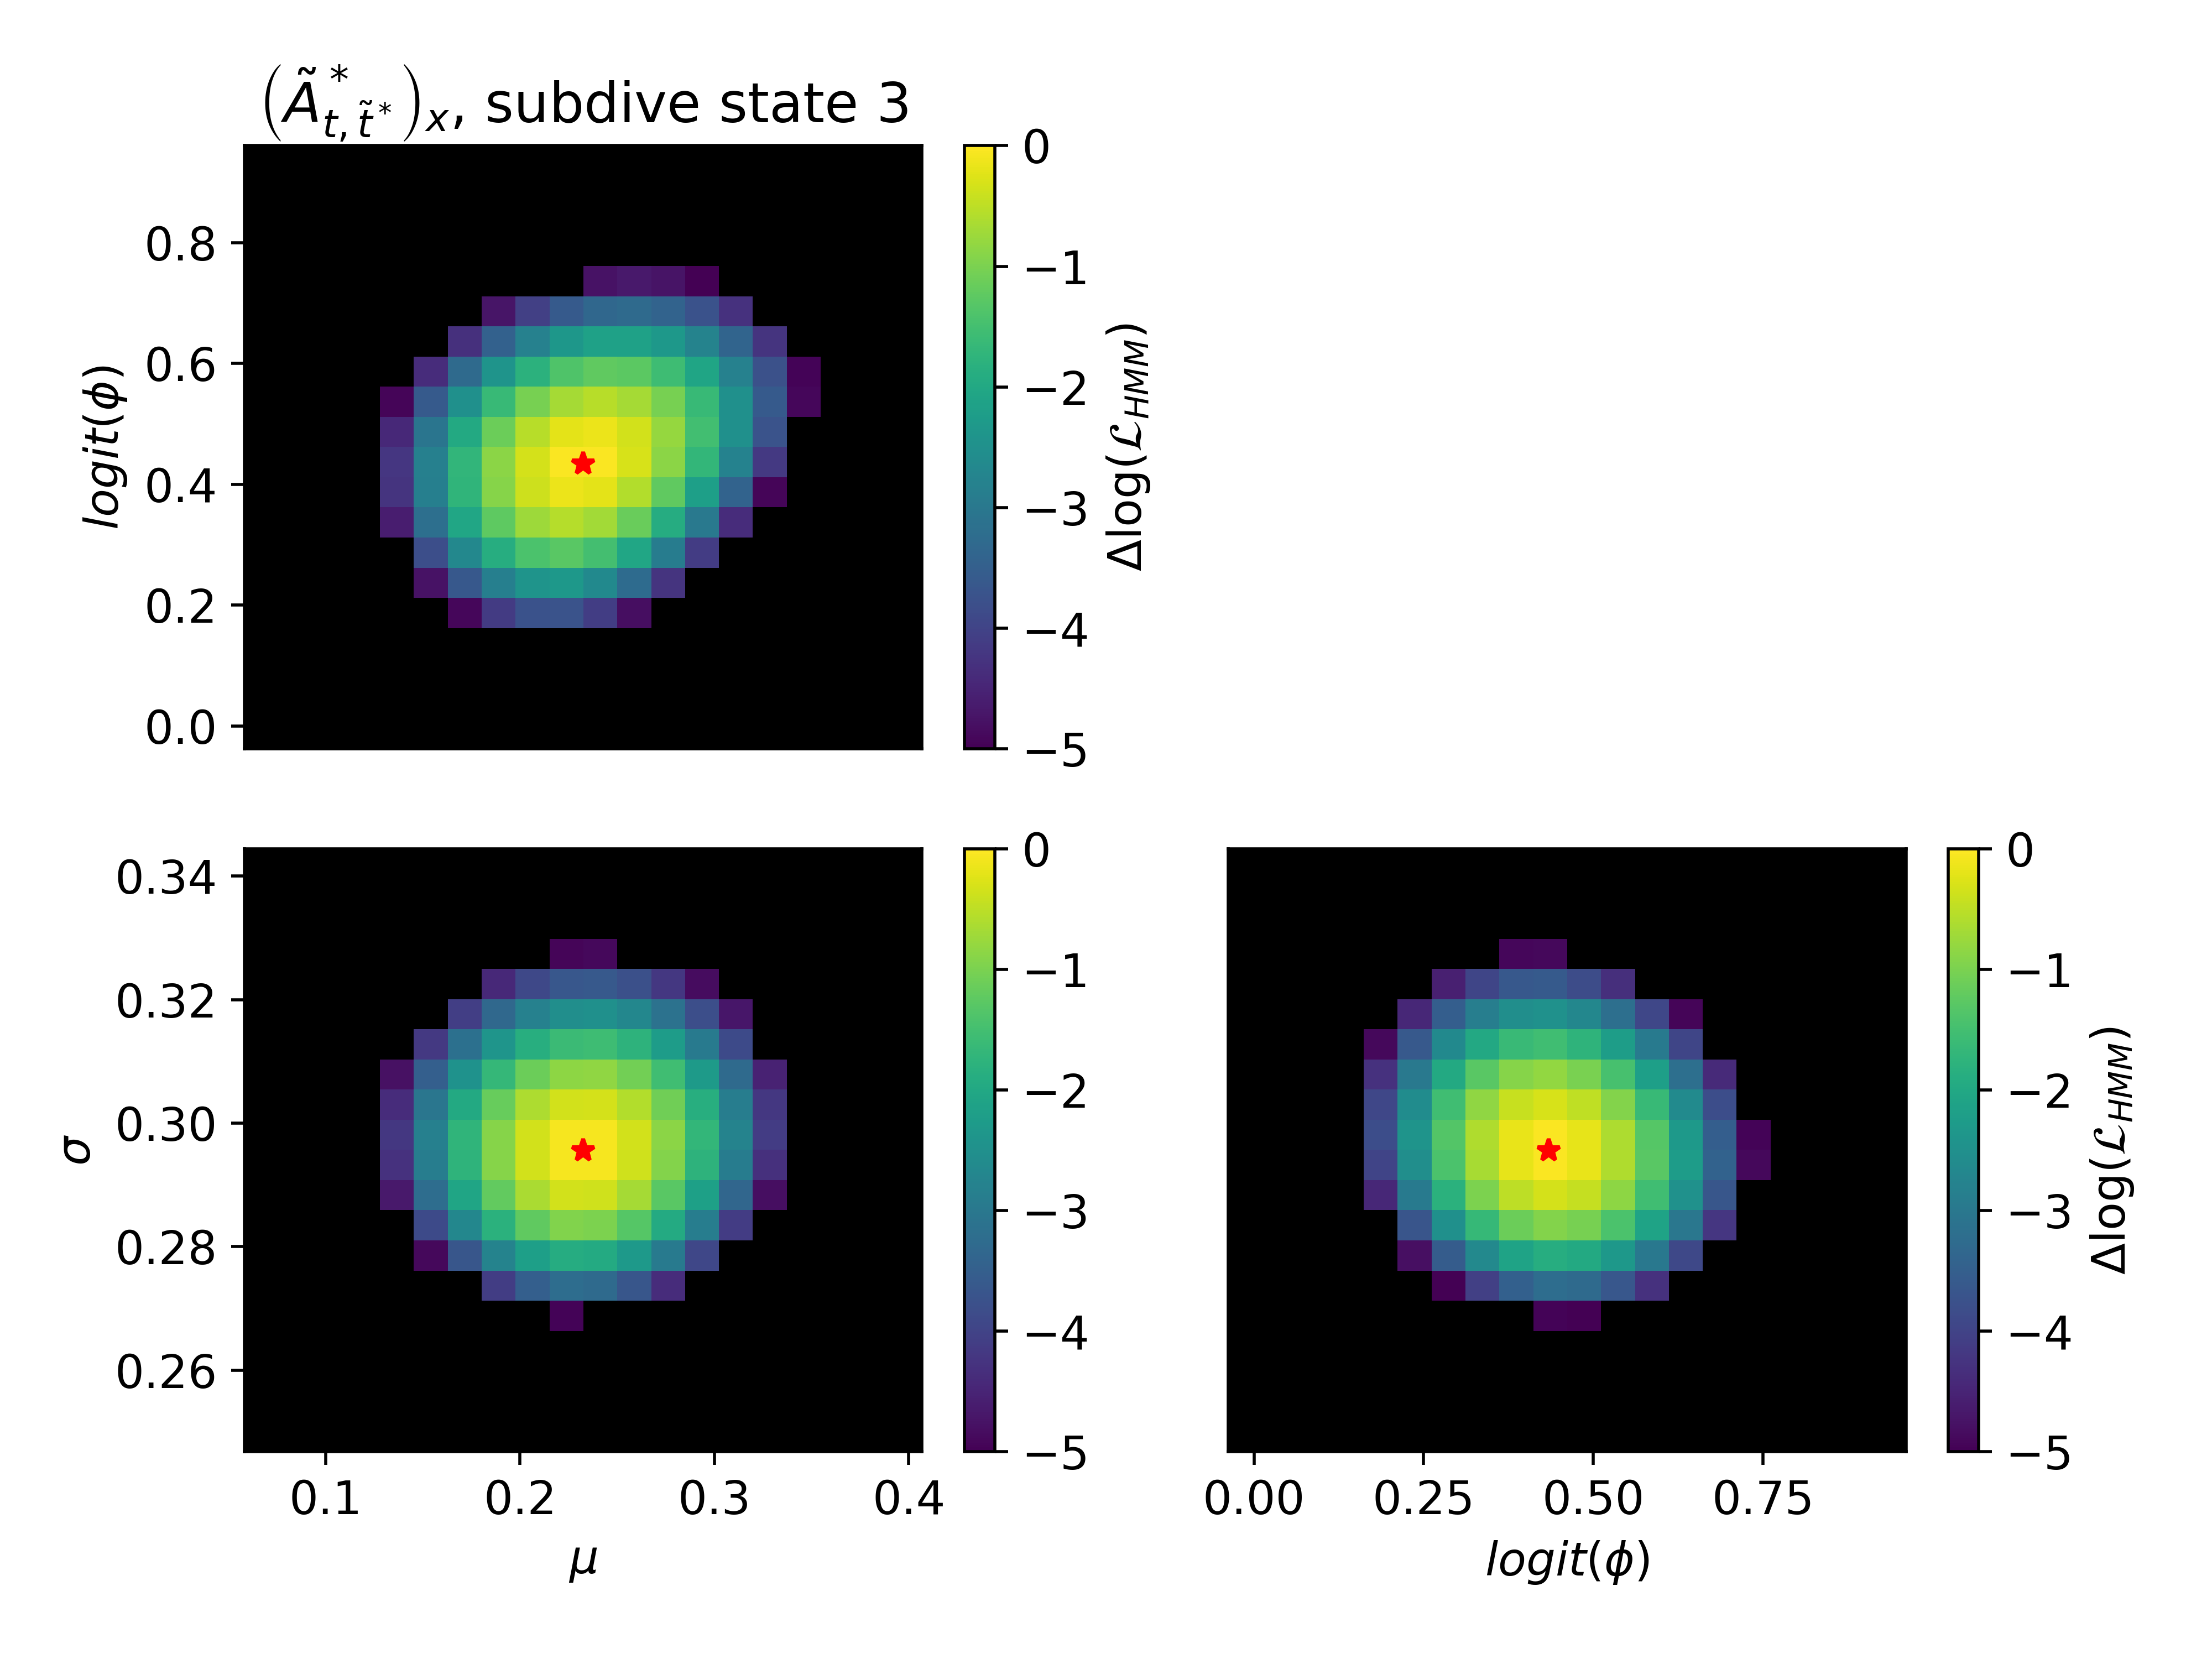
\includegraphics[width=2.1in]{../Plots/2019/20190902-182840-CATs_OB_1_0_267_CarHHMM2_fine-theta-likelihood-Ax-2.png}
        \end{center}
        
        \noindent Figure \arabic{fignum}: Log-likelihood of the CarHHMM-DFT as a function of the $x$-acceleration parameters $\mu_{A_x}^{*(\cdot,i^*)}, \sigma_{A_x}^{*(\cdot,i^*)}$ and logit of $\phi_{A}^{*(\cdot,i^*)}$ for subdive types $i^* = 1,2,3$. All other parameters and probability transition matrices are set to be equal to the maximum likelihood estimates shown in Table (1) of Section 3.1. The log-likelihood is added to the negative log-likelihood of the maximum likelihood estimate $(\hat \mu_{A_x}^{*(\cdot,i^*)}, \hat \sigma_{A_x}^{*(\cdot,i^*)}, \hat \phi_{A}^{*(\cdot,i^*)})$, which is denoted by a red star.
        \addtocounter{fignum}{1}
        
        
        % Ay
        \begin{center}
        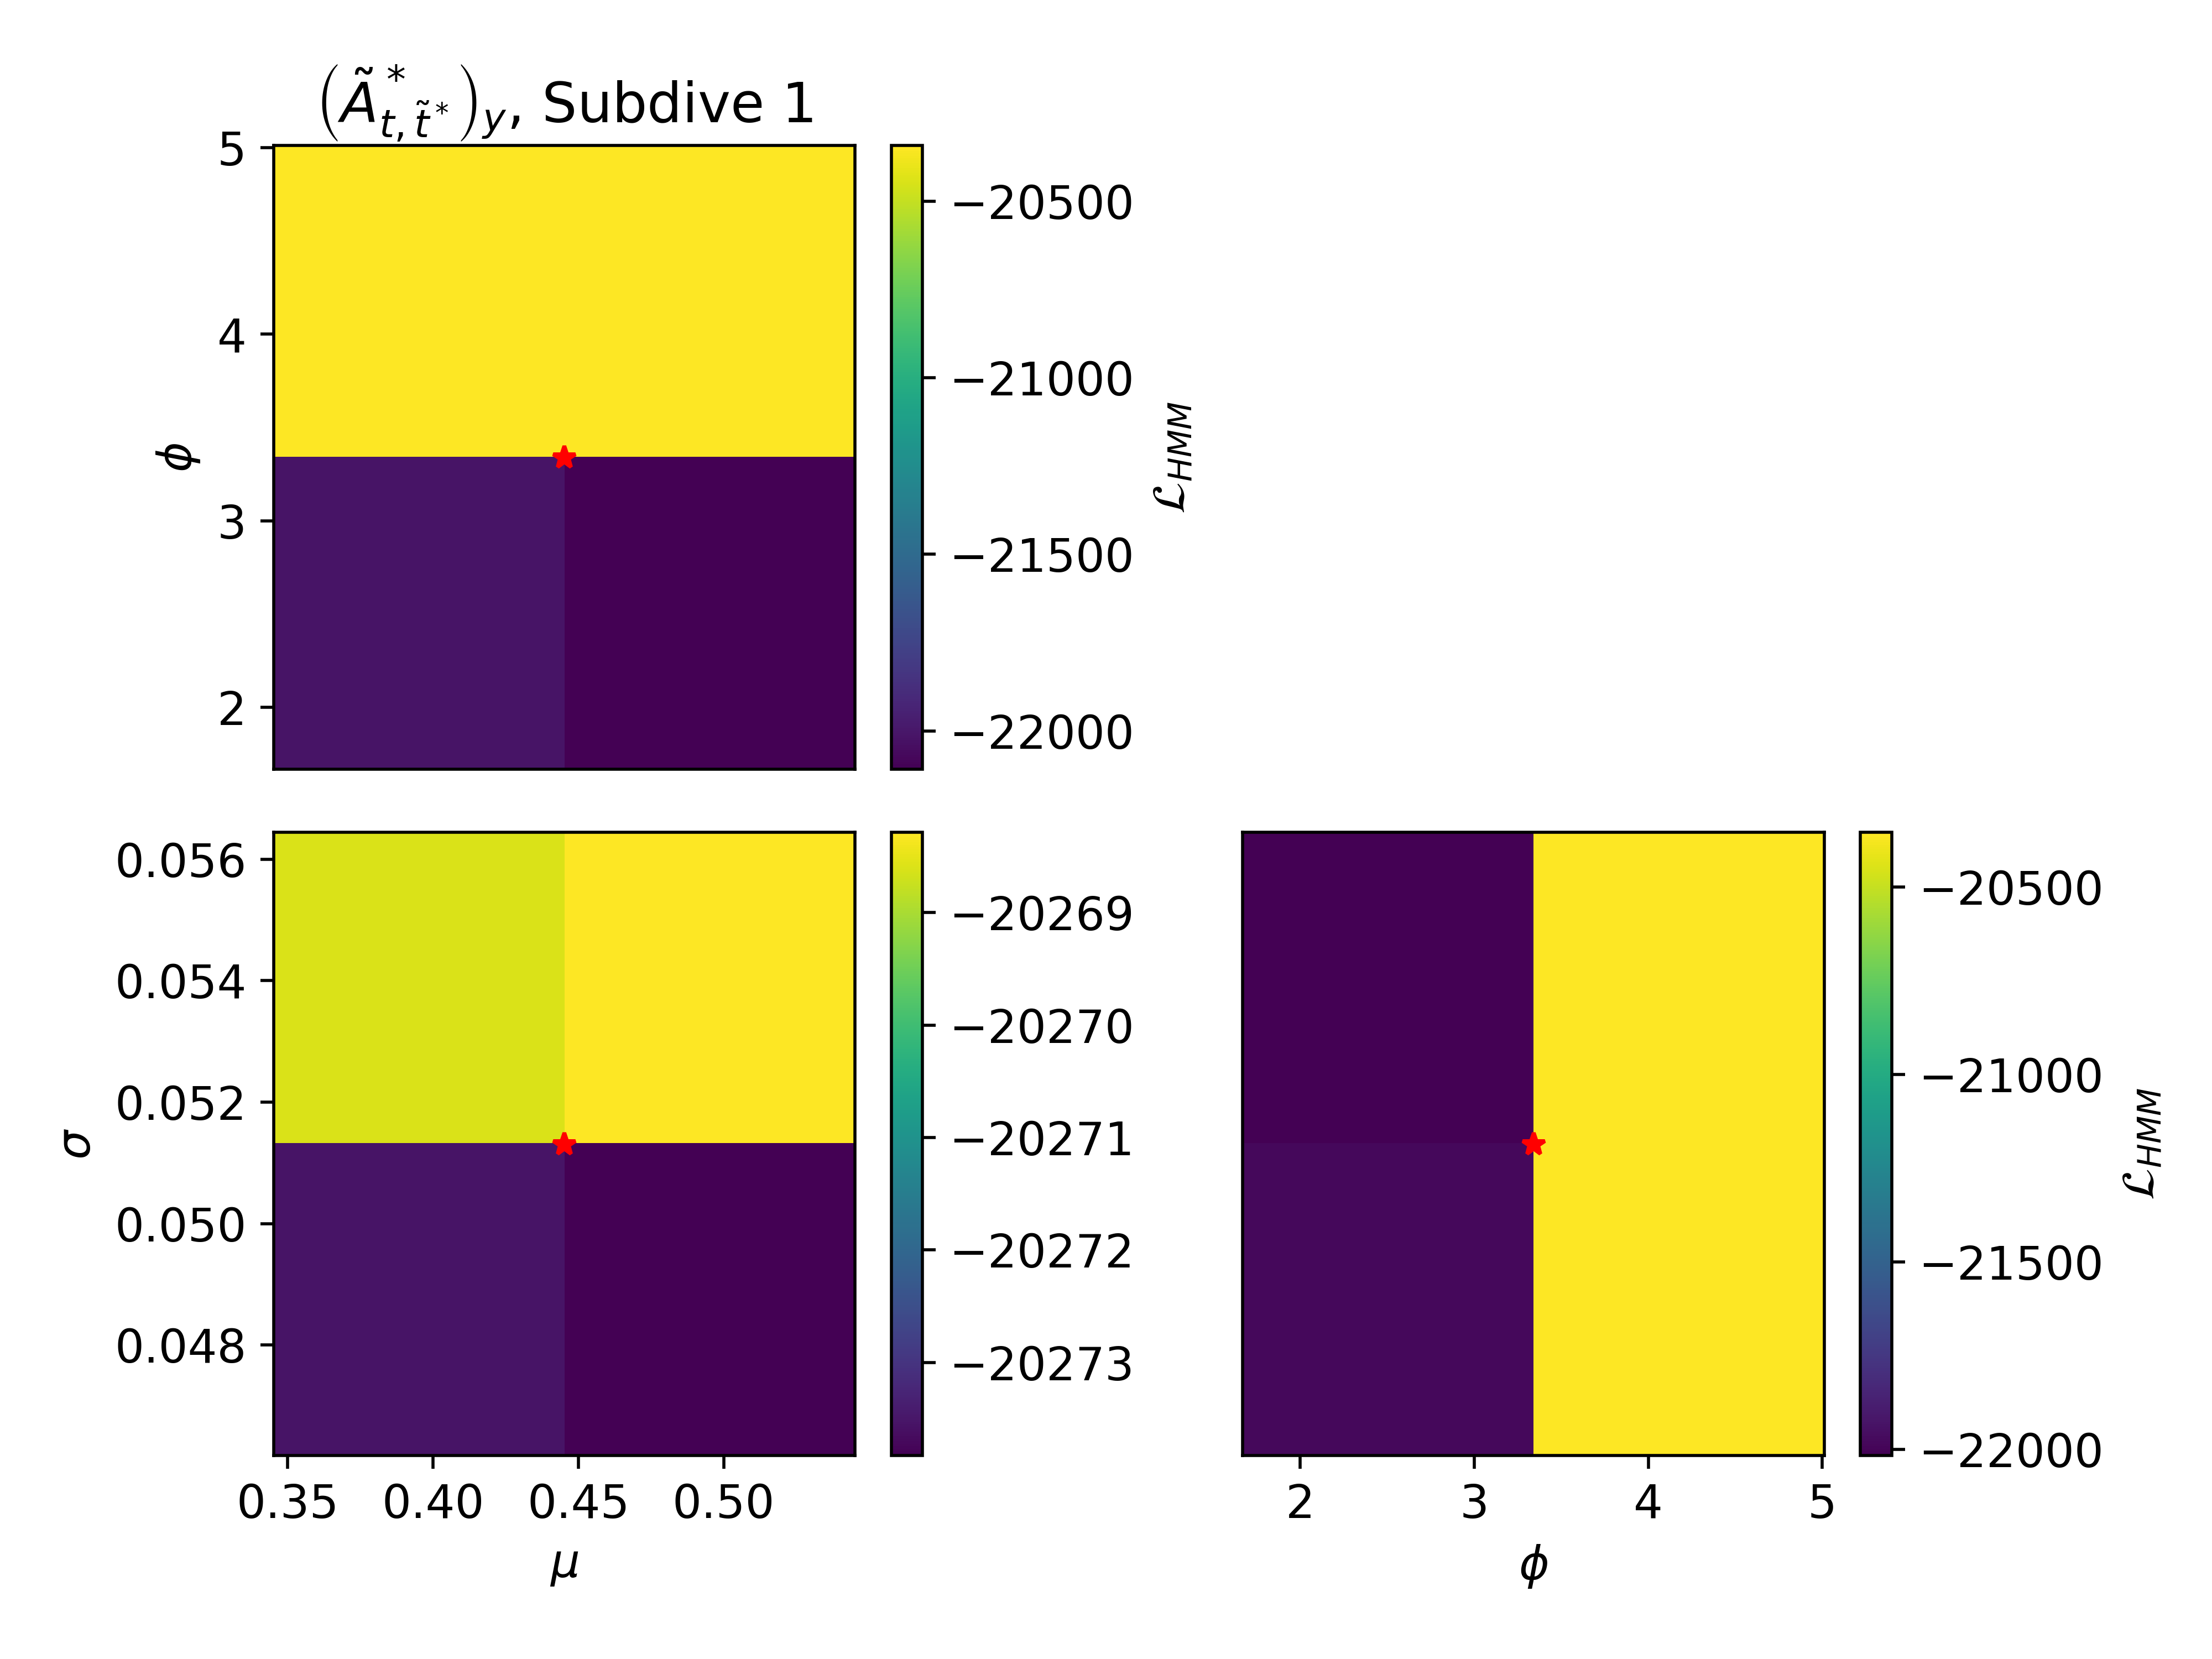
\includegraphics[width=2.1in]{../Plots/2019/20190902-182840-CATs_OB_1_0_267_CarHHMM2_fine-theta-likelihood-Ay-0.png}
        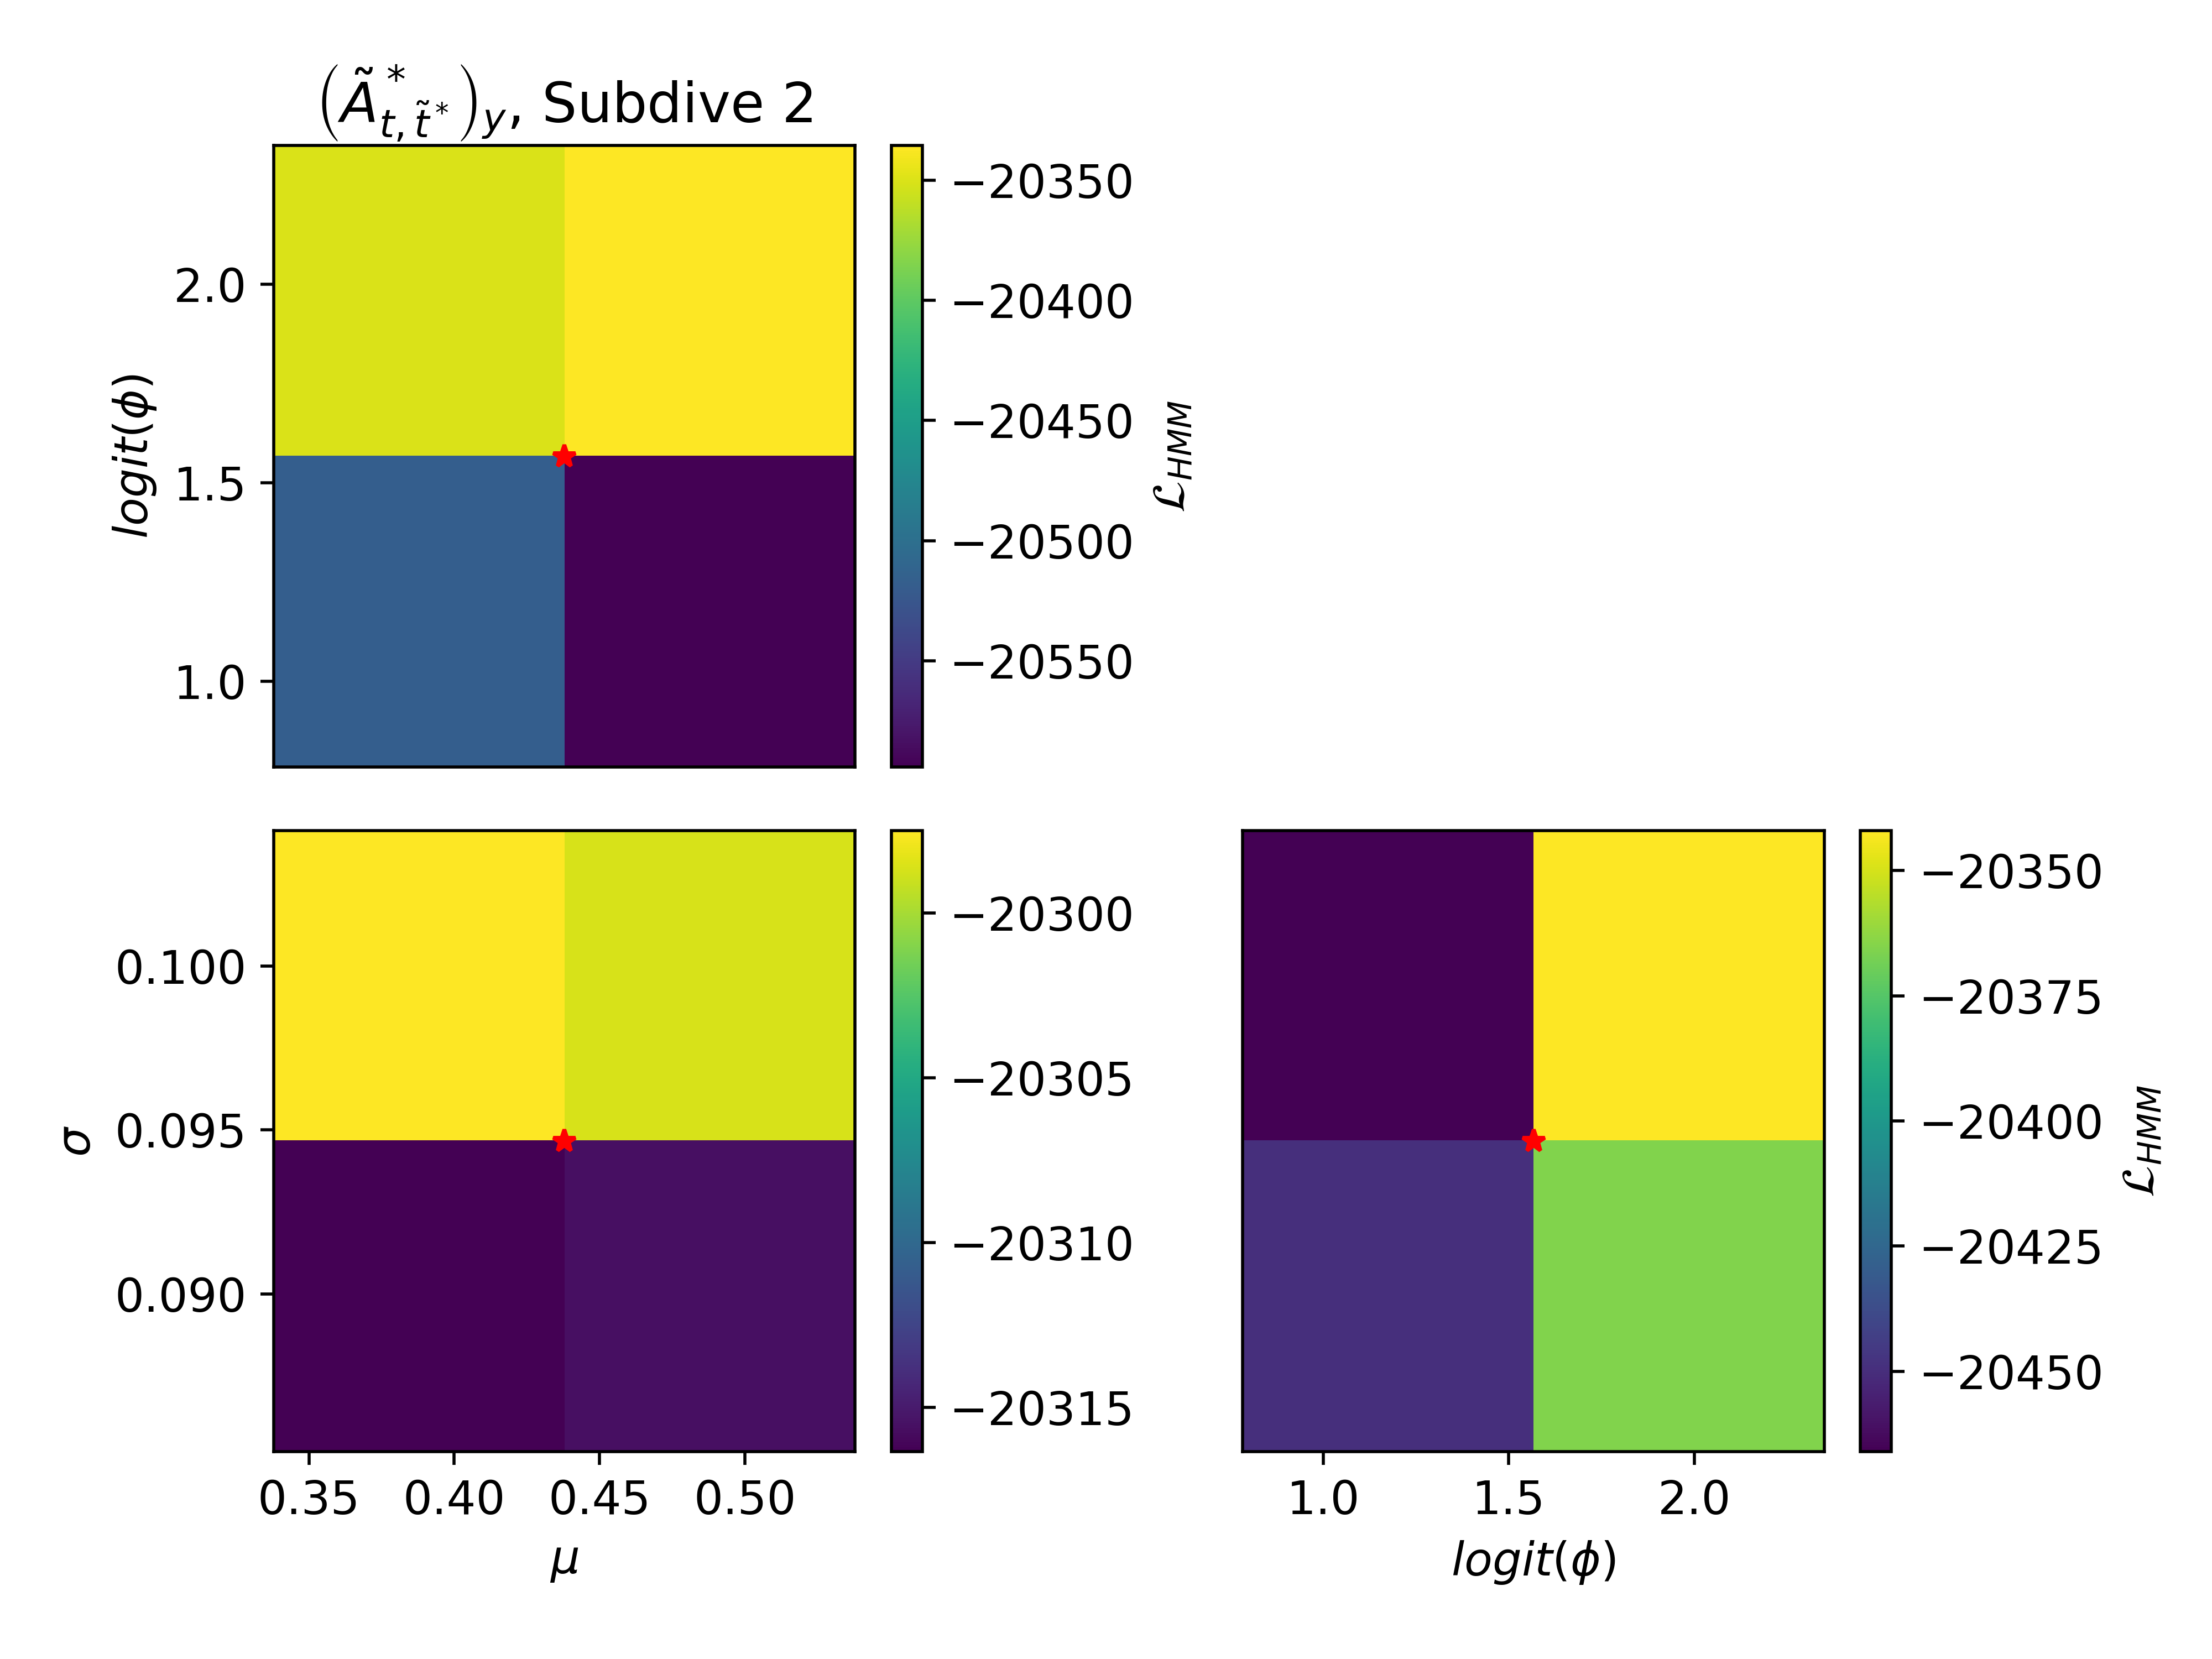
\includegraphics[width=2.1in]{../Plots/2019/20190902-182840-CATs_OB_1_0_267_CarHHMM2_fine-theta-likelihood-Ay-1.png}
        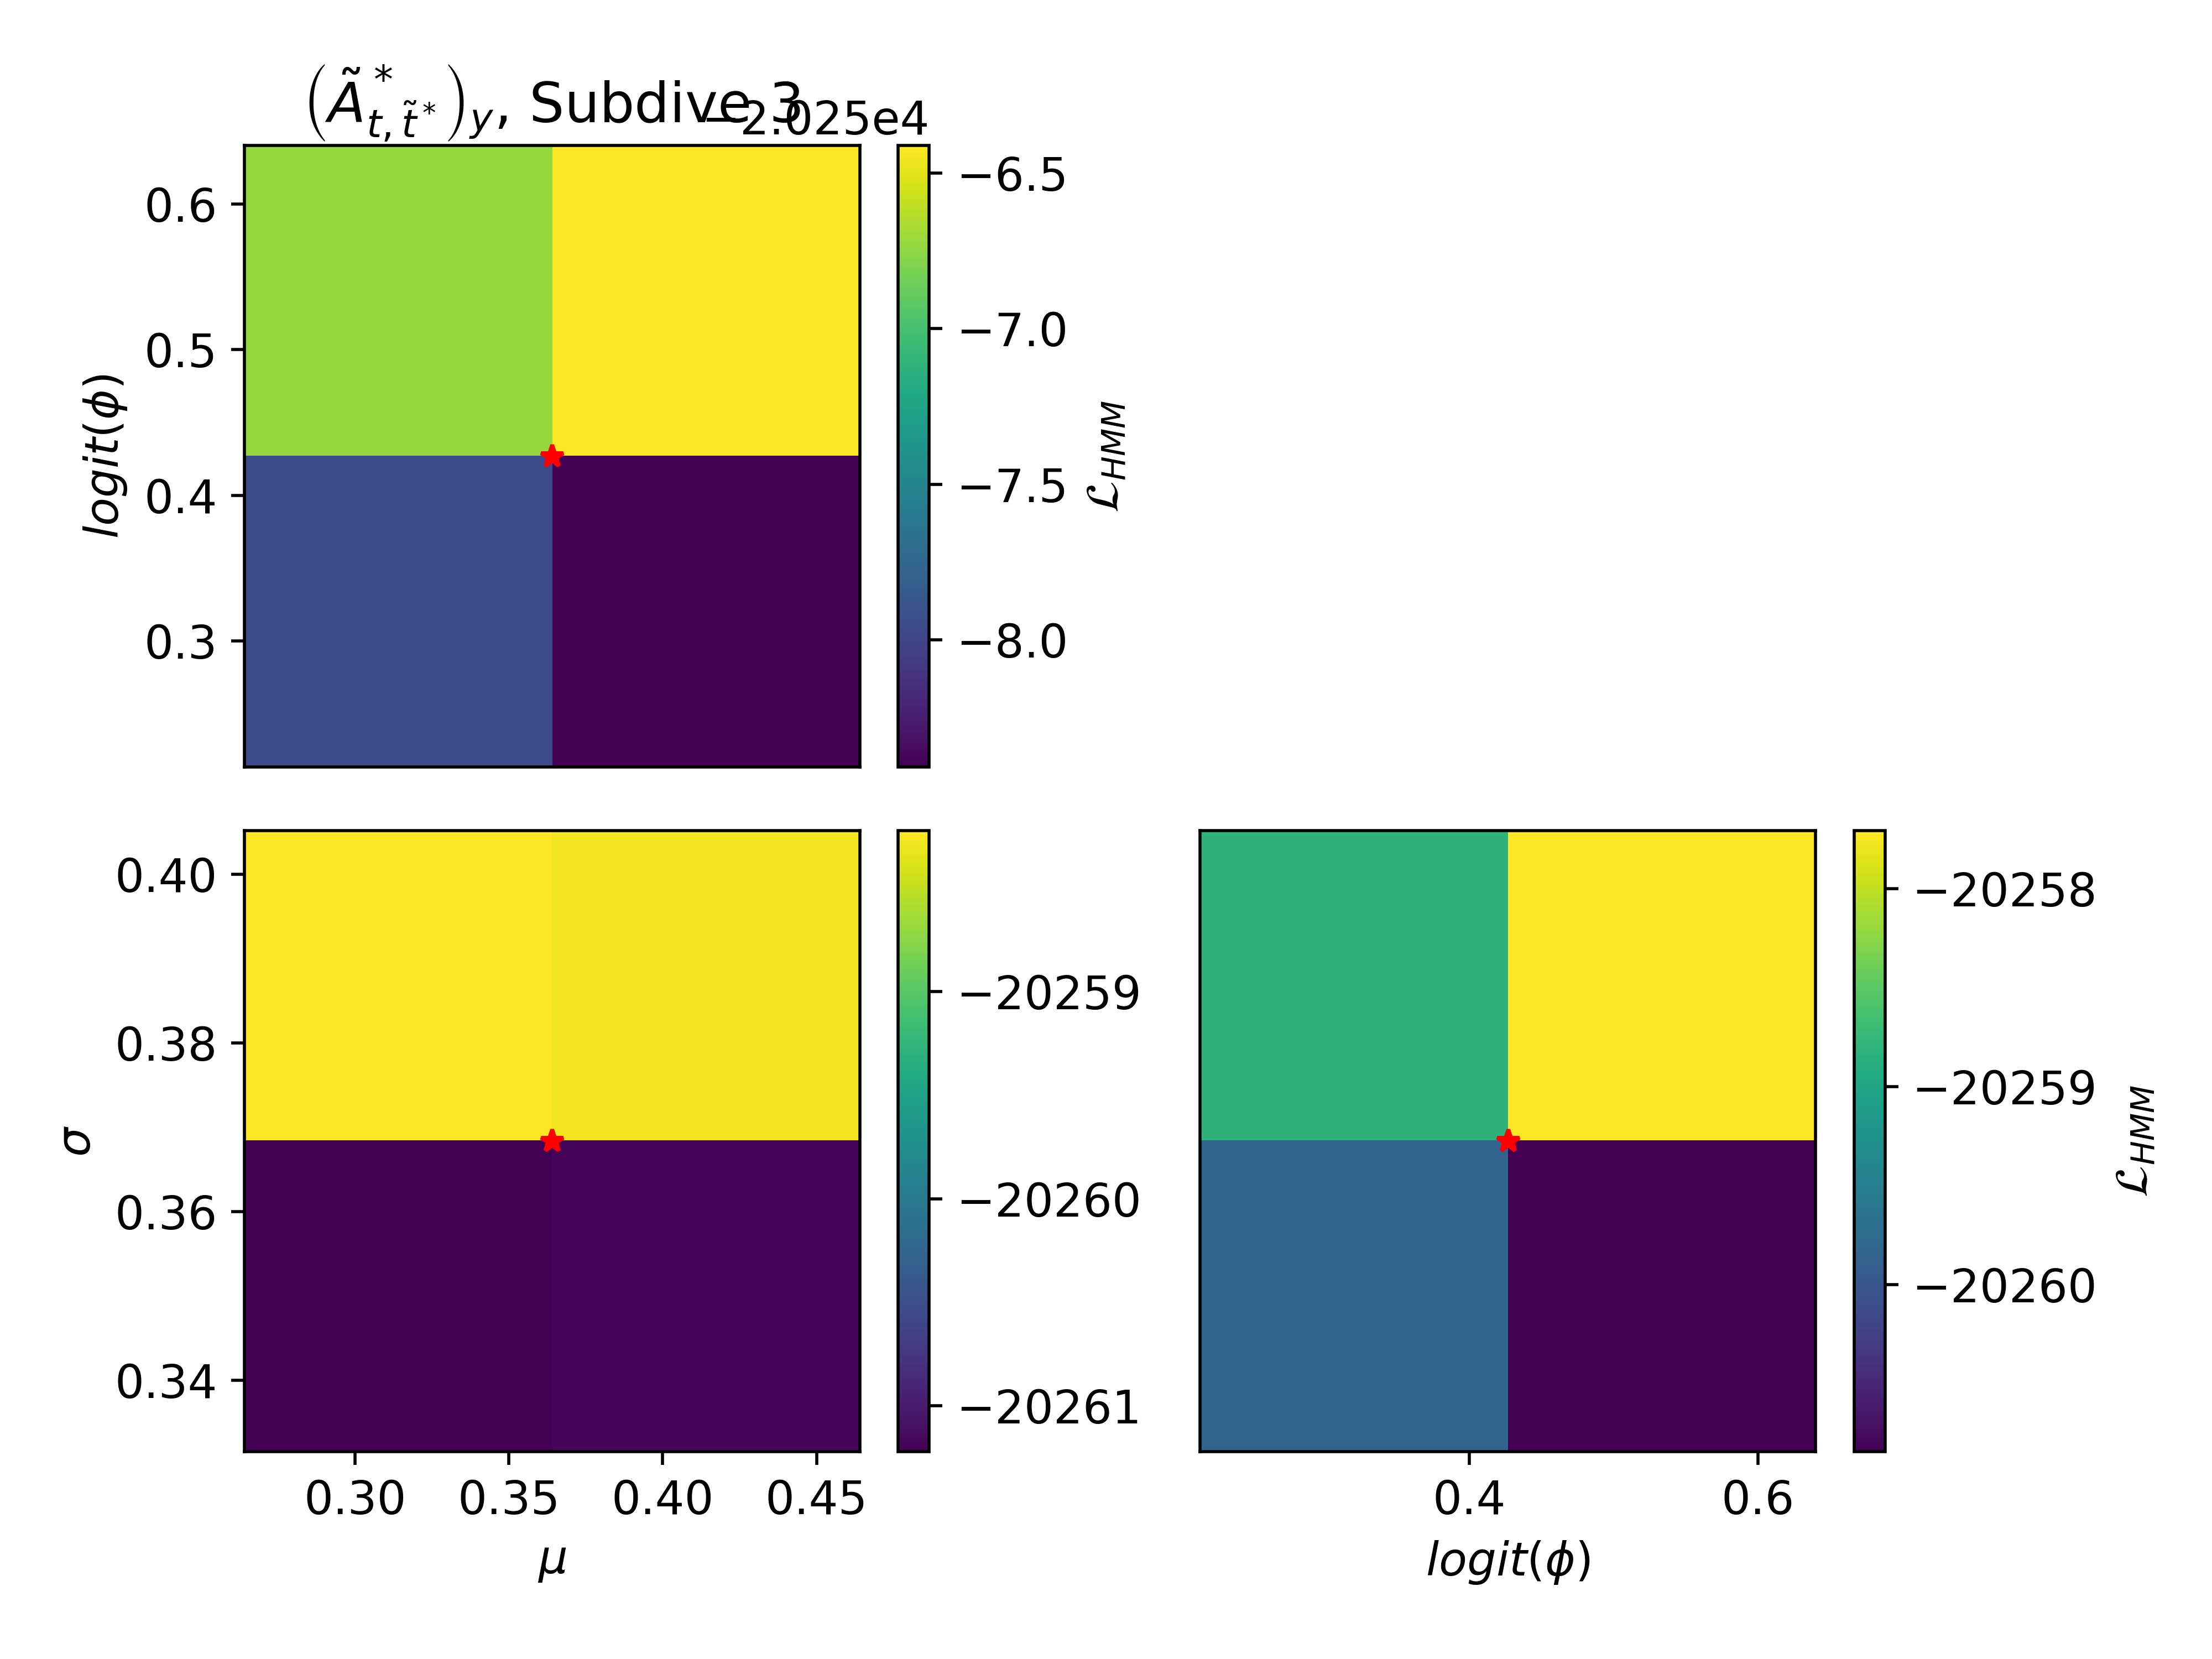
\includegraphics[width=2.1in]{../Plots/2019/20190902-182840-CATs_OB_1_0_267_CarHHMM2_fine-theta-likelihood-Ay-2.png}
        \end{center}
        
        \noindent Figure \arabic{fignum}: Log-likelihood of the CarHHMM-DFT as a function of the $y$-acceleration parameters $\mu_{A_y}^{*(\cdot,i^*)}, \sigma_{A_y}^{*(\cdot,i^*)}$ and logit of $\phi_{A}^{*(\cdot,i^*)}$ for subdive types $i^* = 1,2,3$. All other parameters and probability transition matrices are set to be equal to the maximum likelihood estimates shown in Table (1) of Section 3.1. The log-likelihood is added to the negative log-likelihood of the maximum likelihood estimate $(\hat \mu_{A_y}^{*(\cdot,i^*)}, \hat \sigma_{A_y}^{*(\cdot,i^*)}, \hat \phi_{A}^{*(\cdot,i^*)})$, which is denoted by a red star.
        \addtocounter{fignum}{1}
        
        % Az
        \begin{center}
        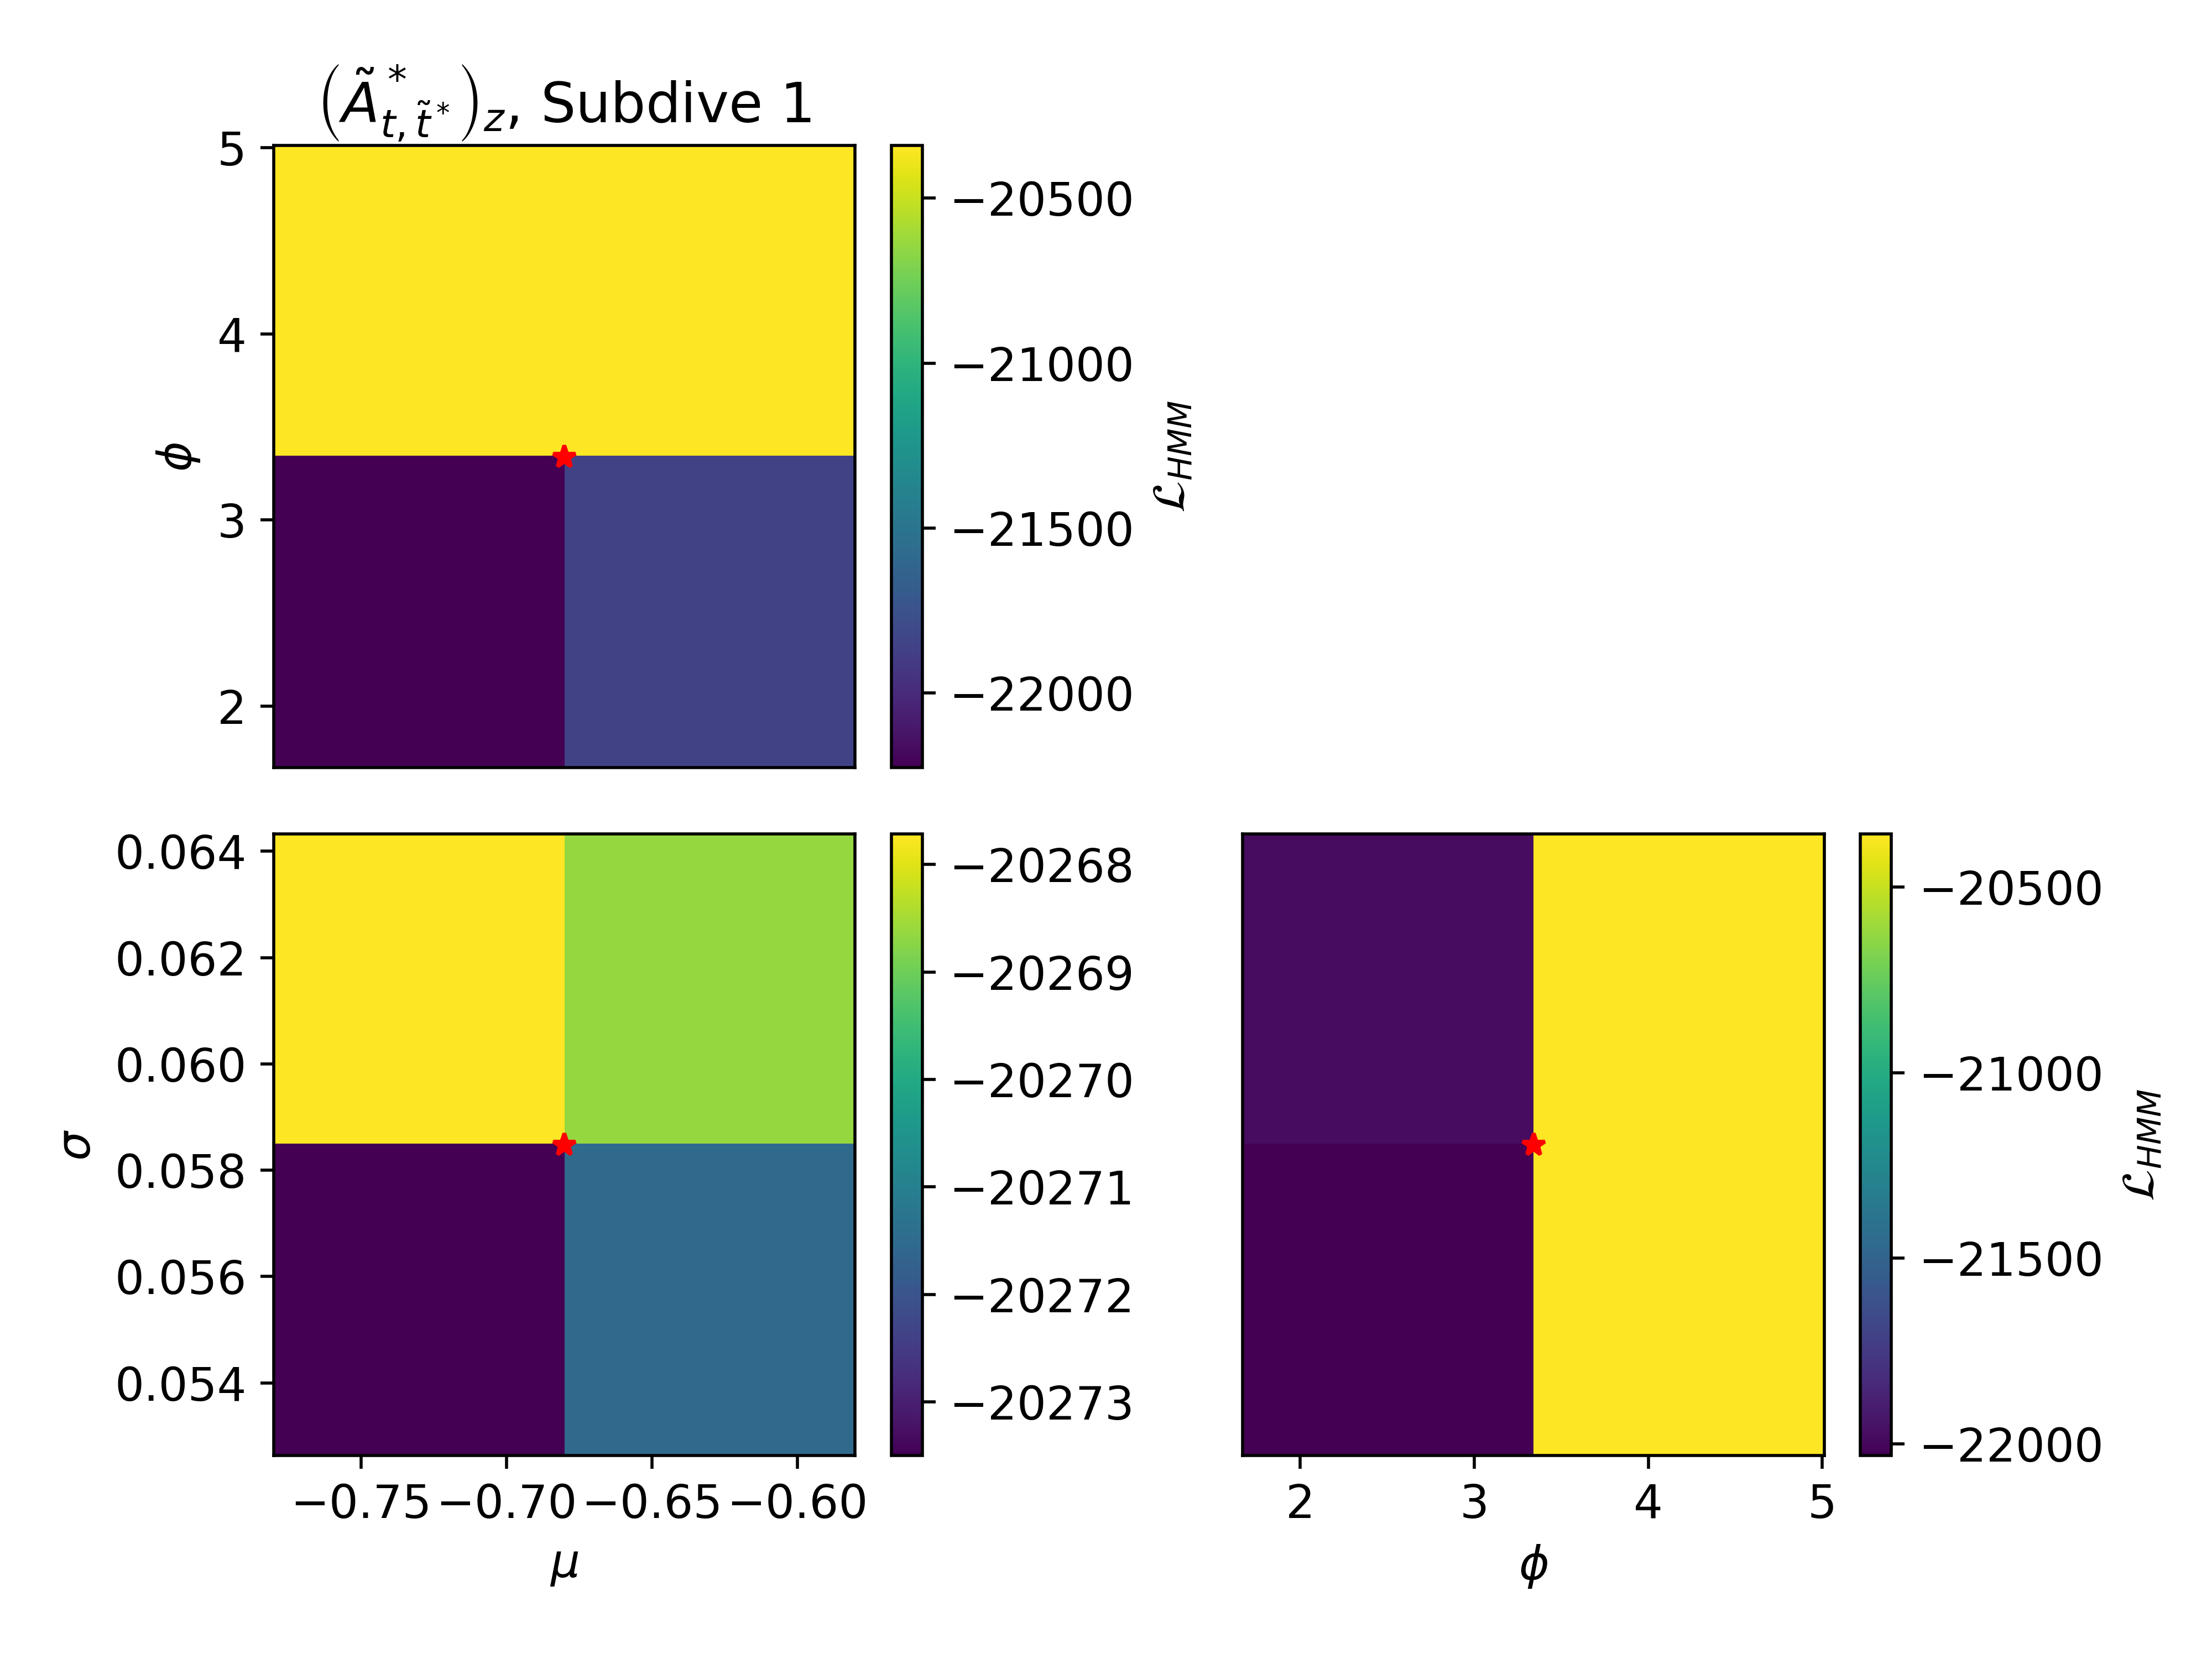
\includegraphics[width=2.1in]{../Plots/2019/20190902-182840-CATs_OB_1_0_267_CarHHMM2_fine-theta-likelihood-Az-0.png}
        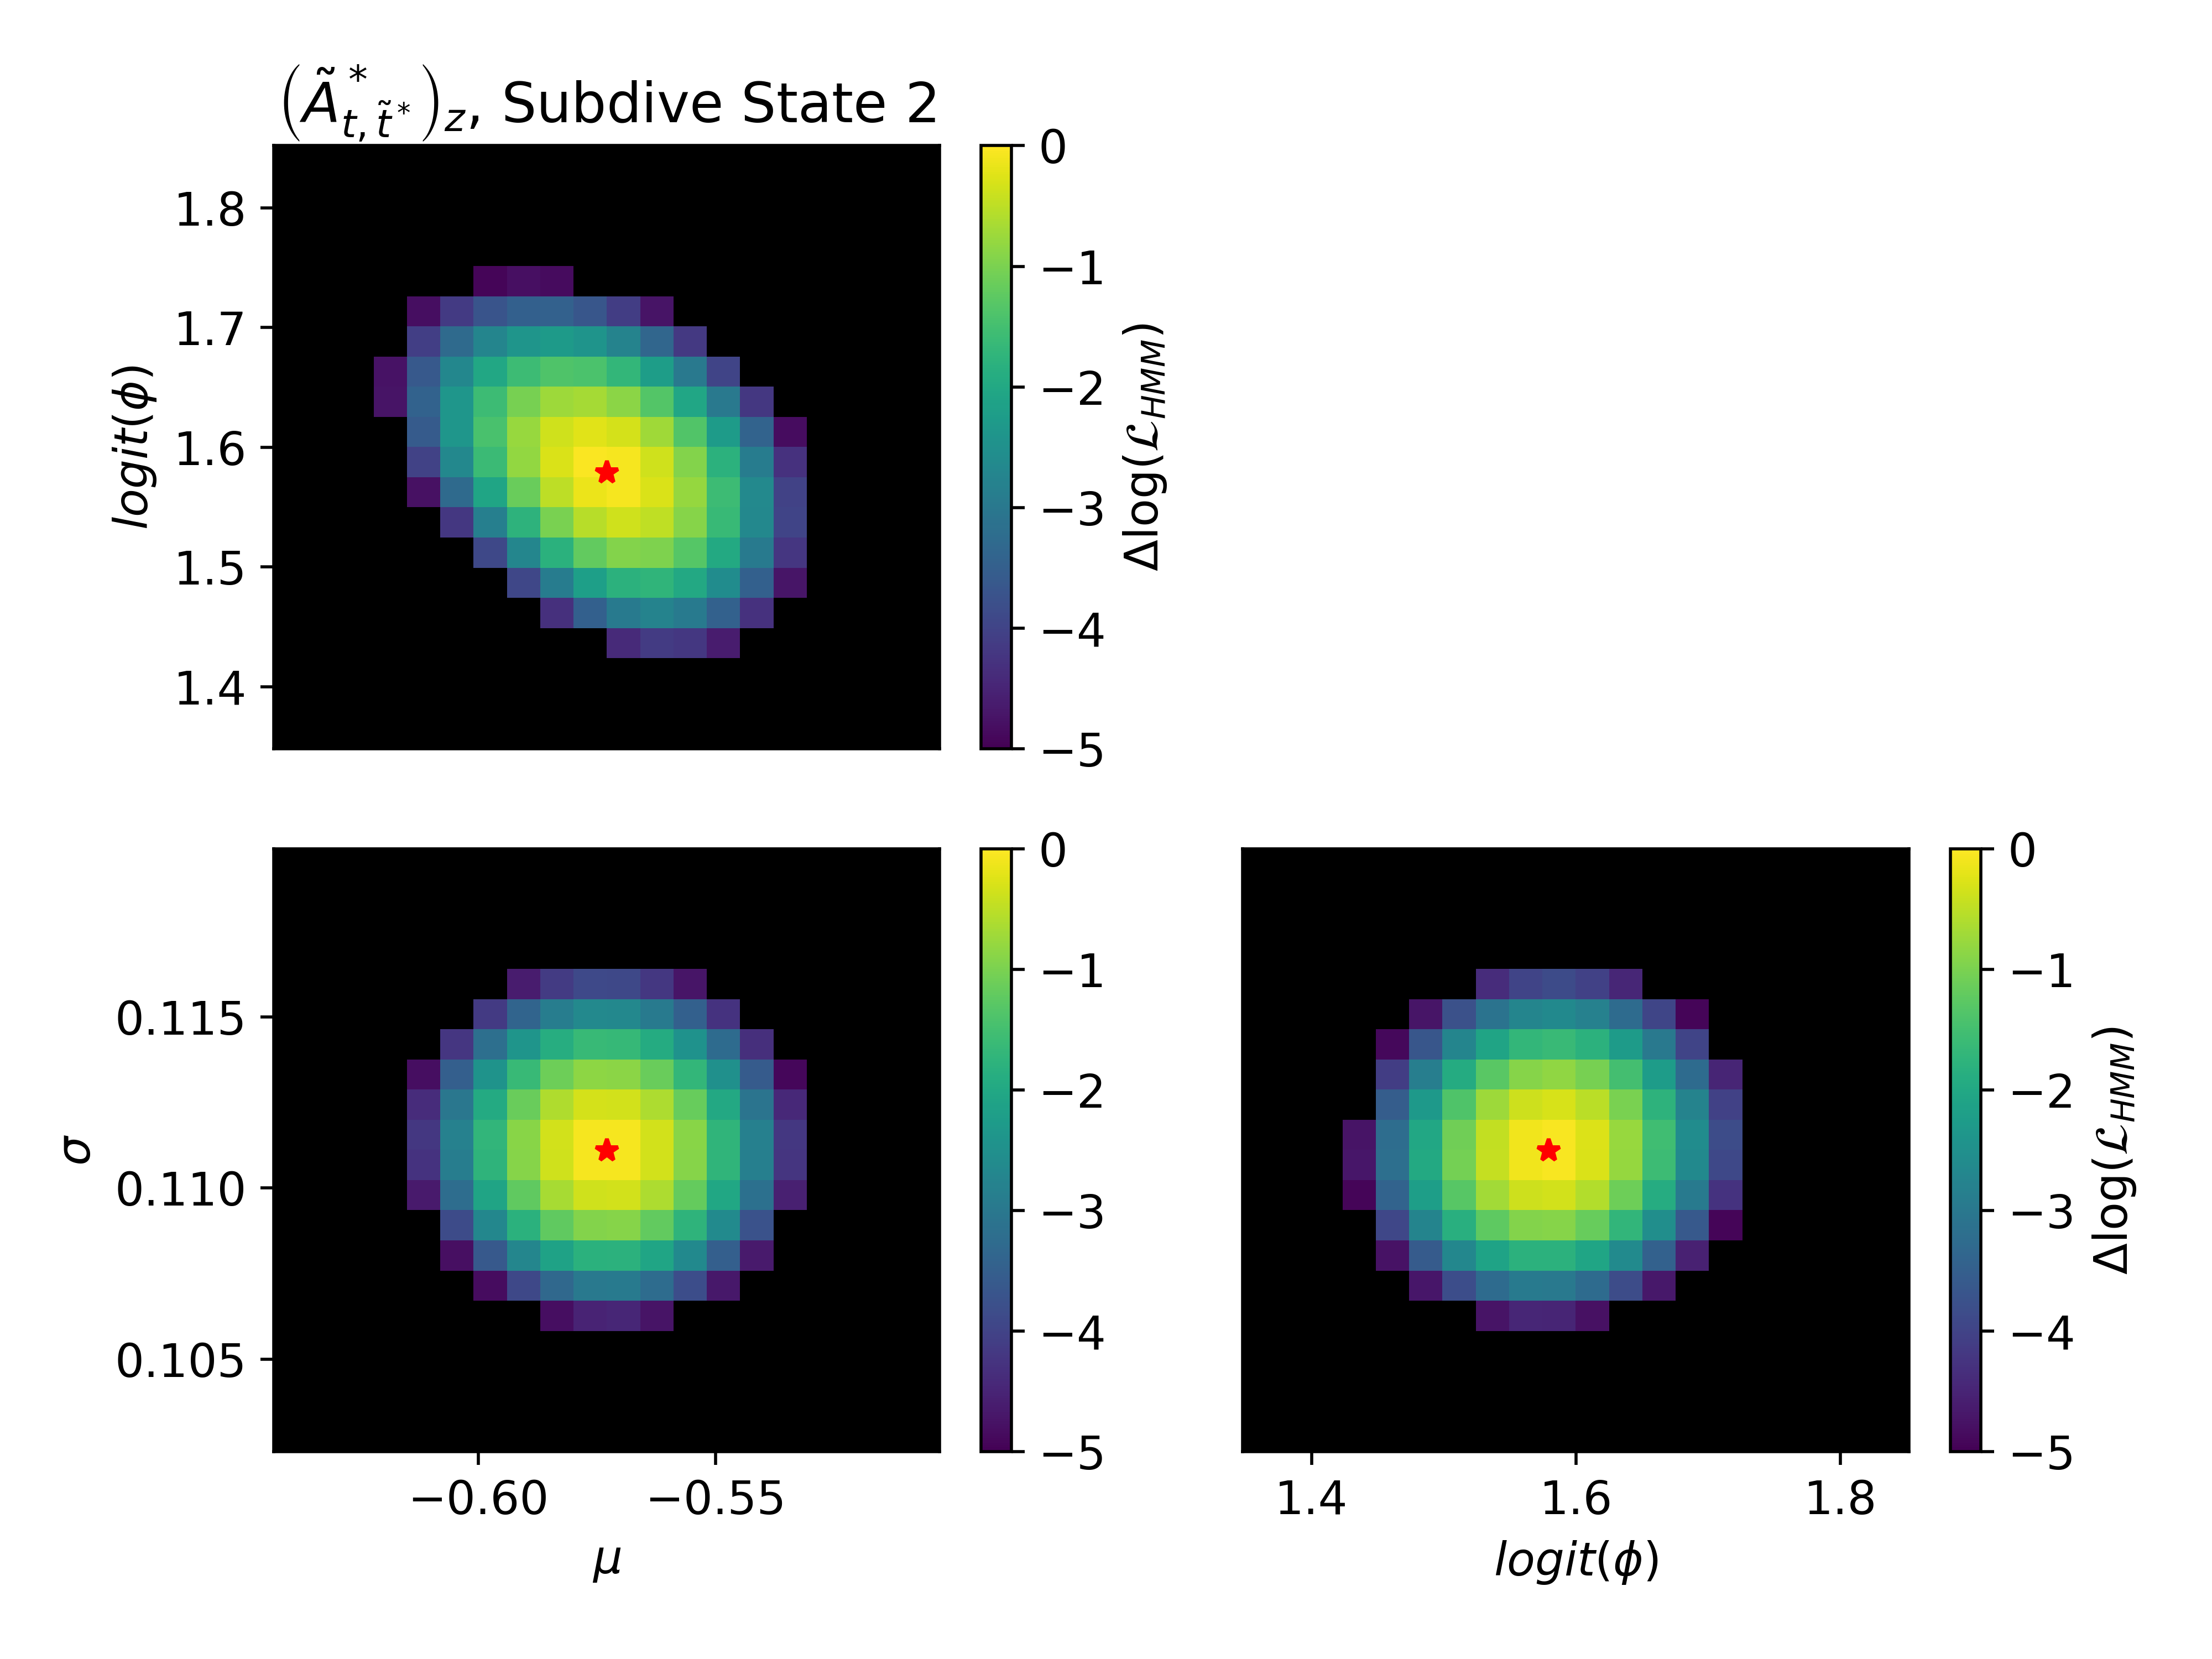
\includegraphics[width=2.1in]{../Plots/2019/20190902-182840-CATs_OB_1_0_267_CarHHMM2_fine-theta-likelihood-Az-1.png}
        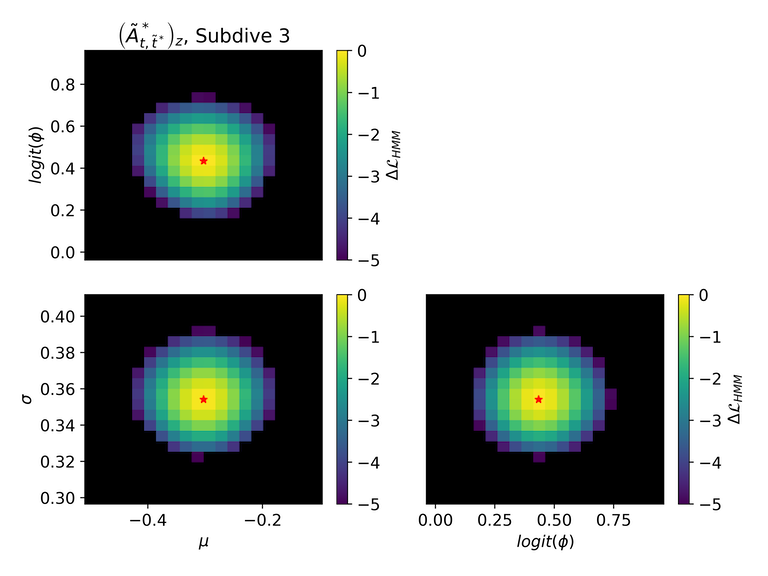
\includegraphics[width=2.1in]{../Plots/2019/20190902-182840-CATs_OB_1_0_267_CarHHMM2_fine-theta-likelihood-Az-2.png}
        \end{center}
        
        \noindent Figure \arabic{fignum}: Log-likelihood of the CarHHMM-DFT as a function of the $z$-acceleration parameters $\mu_{A_z}^{*(\cdot,i^*)}, \sigma_{A_z}^{*(\cdot,i^*)}$ and logit of $\phi_{A}^{*(\cdot,i^*)}$ for subdive types $i^* = 1,2,3$. All other parameters and probability transition matrices are set to be equal to the maximum likelihood estimates shown in Table (1) of Section 3.1. The log-likelihood is added to the negative log-likelihood of the maximum likelihood estimate $(\hat \mu_{A_z}^{*(\cdot,i^*)}, \hat \sigma_{A_z}^{*(\cdot,i^*)}, \hat \phi_{A}^{*(\cdot,i^*)})$, which is denoted by a red star.
        \addtocounter{fignum}{1}
        
        \newpage
        
        % eta1
        \begin{center}
        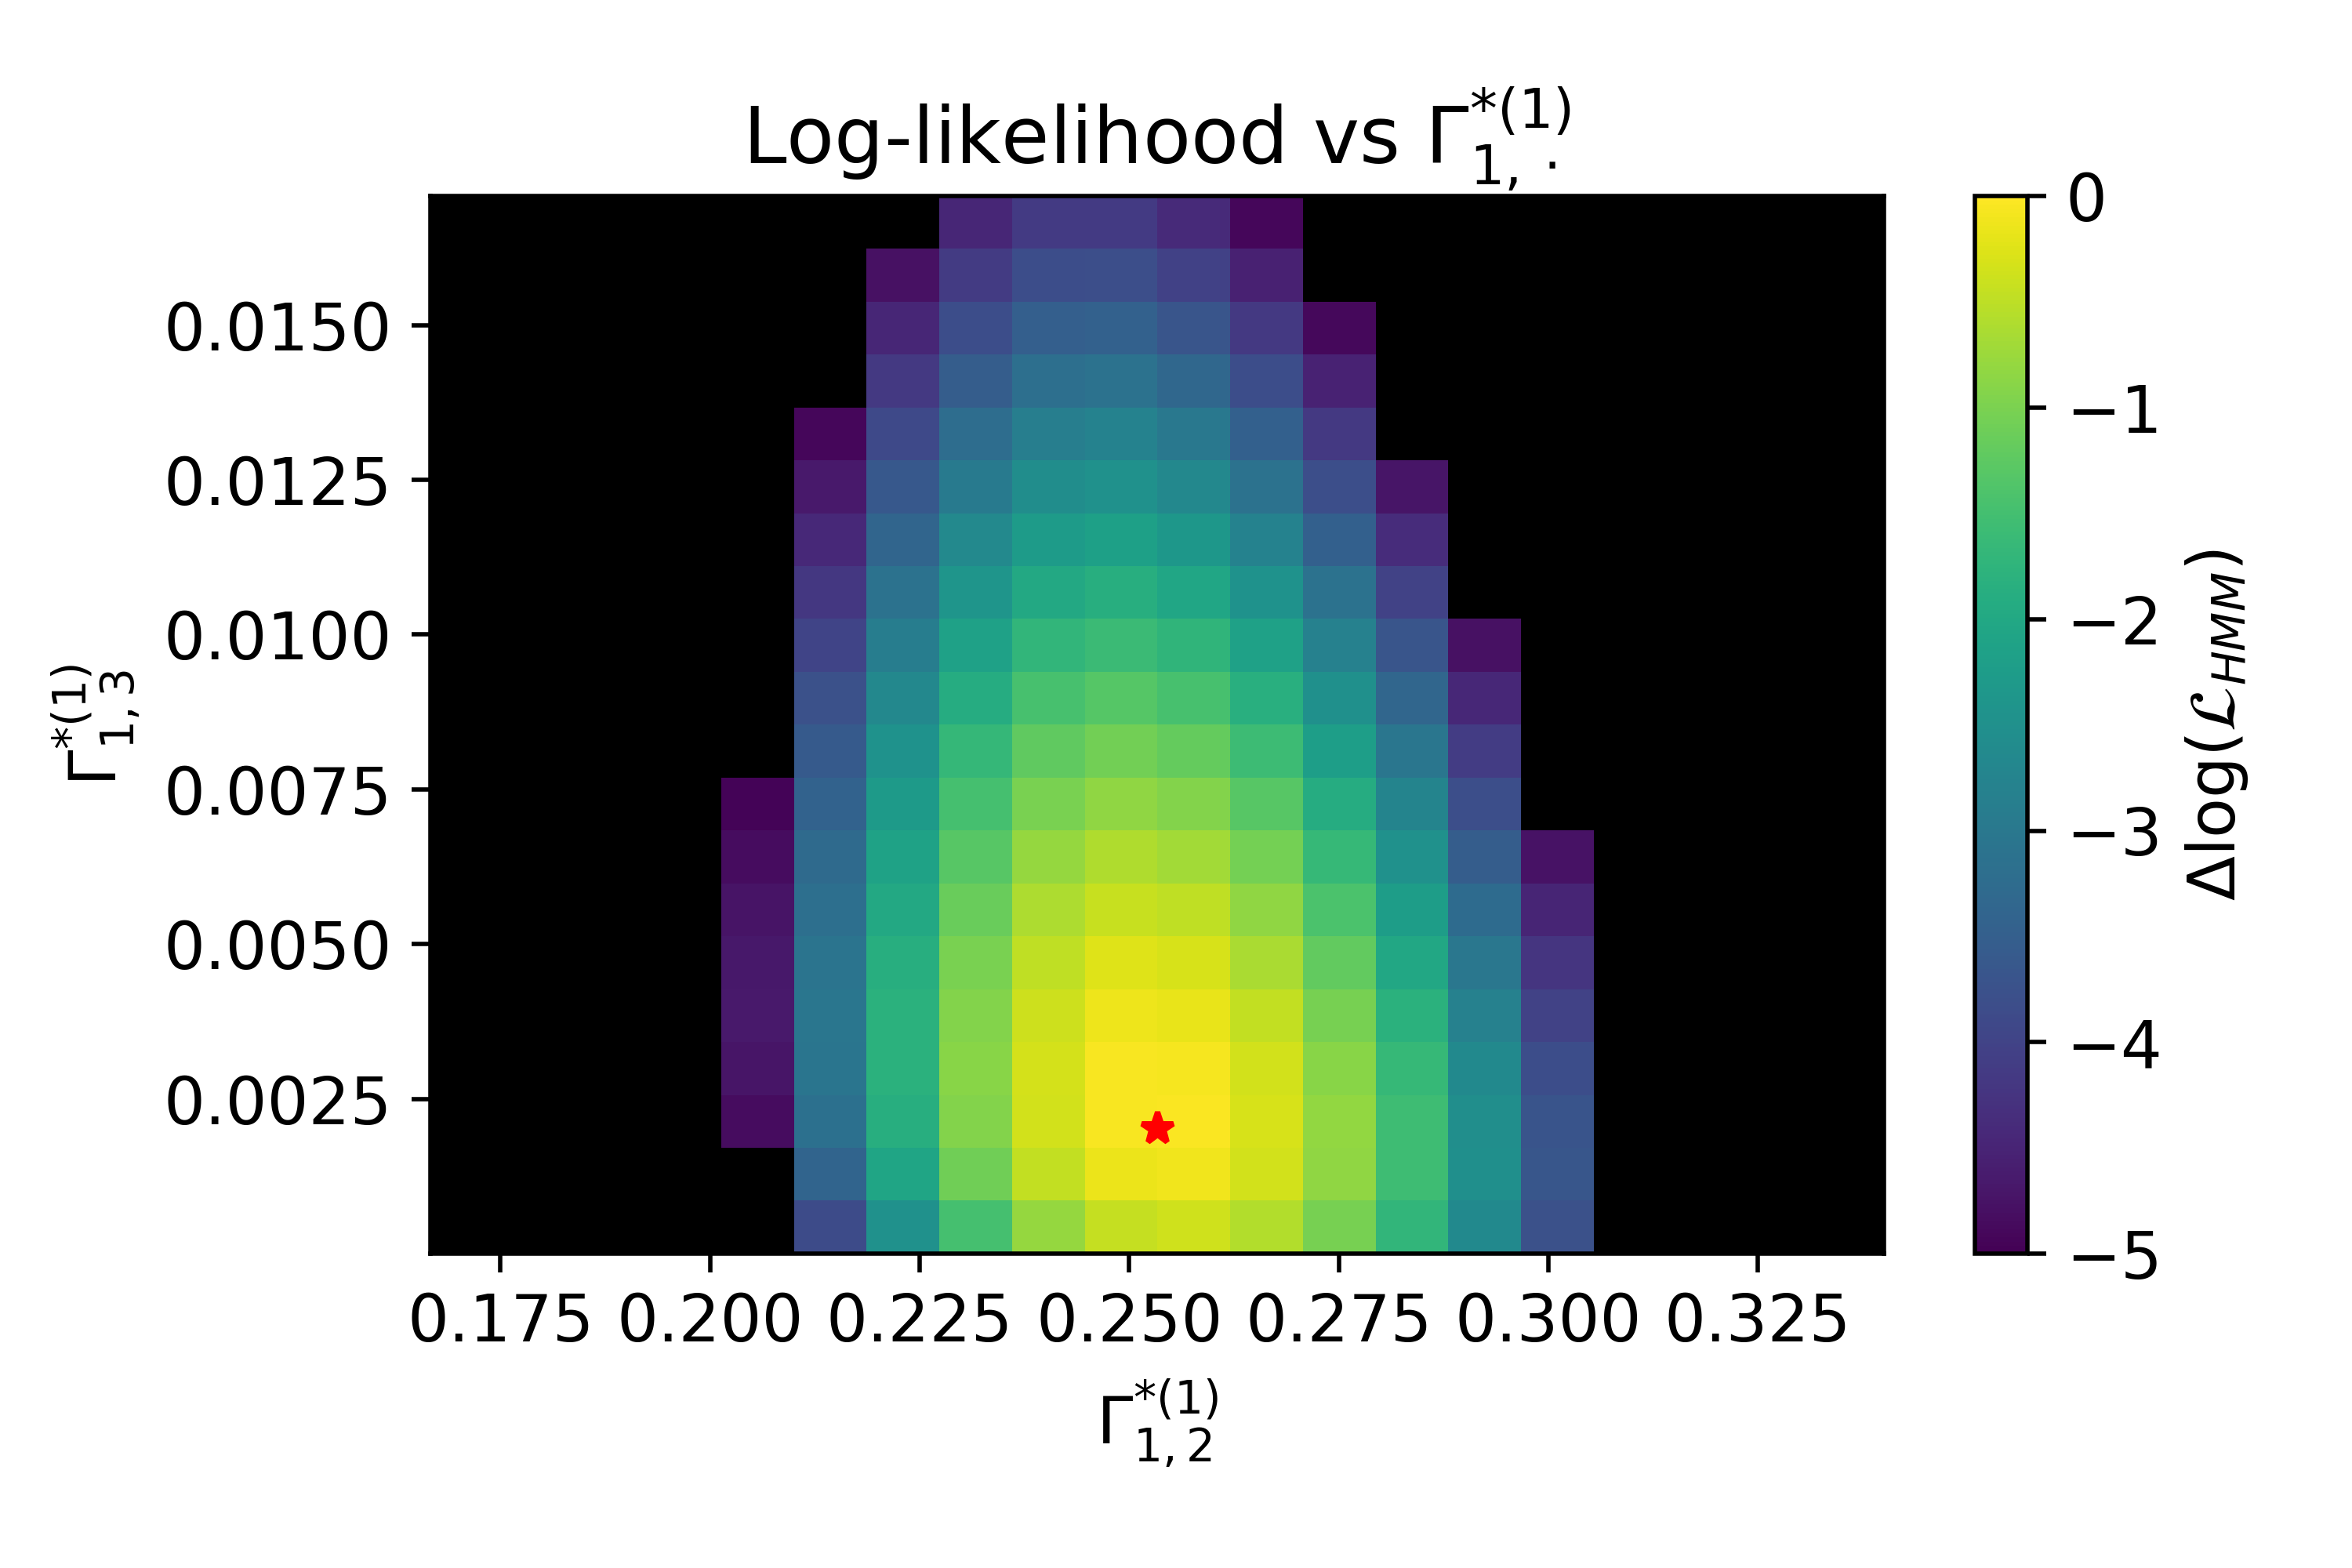
\includegraphics[width=3in]{../Plots/2019/20190902-182840-CATs_OB_1_0_267_CarHHMM2_fine-gamma-likelihood-0-row_0.png}
        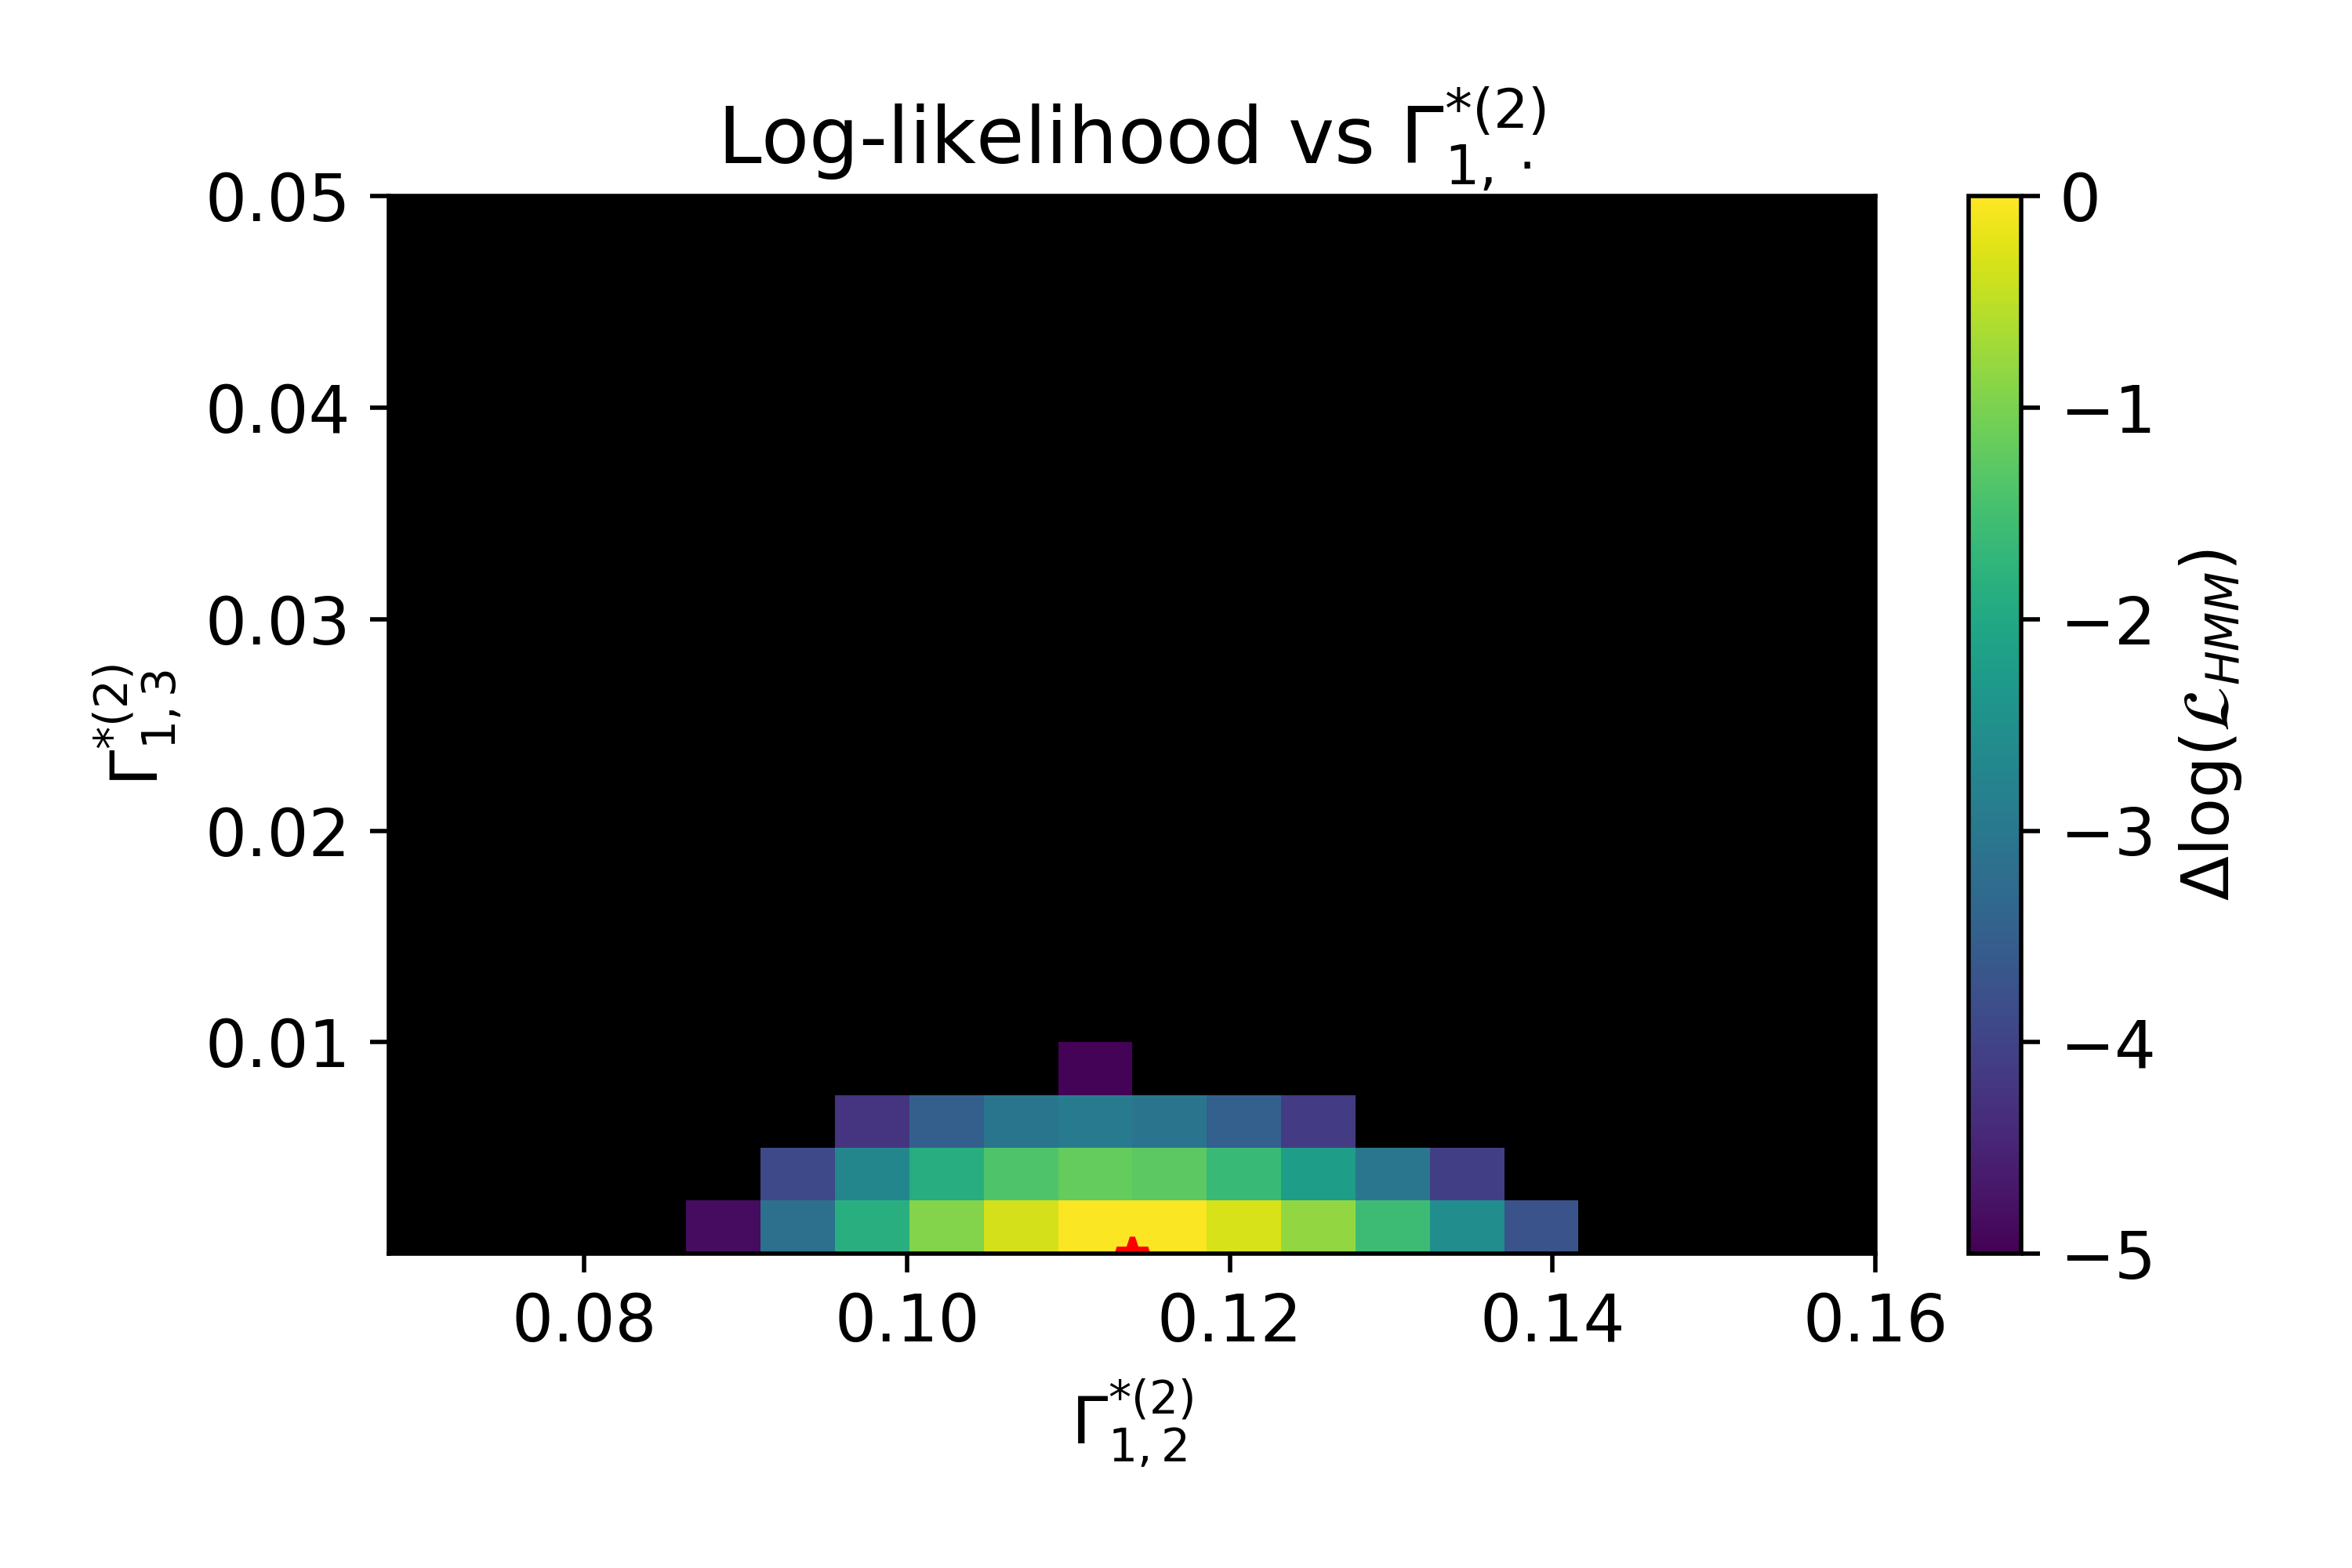
\includegraphics[width=3in]{../Plots/2019/20190902-182840-CATs_OB_1_0_267_CarHHMM2_fine-gamma-likelihood-1-row_0.png}
        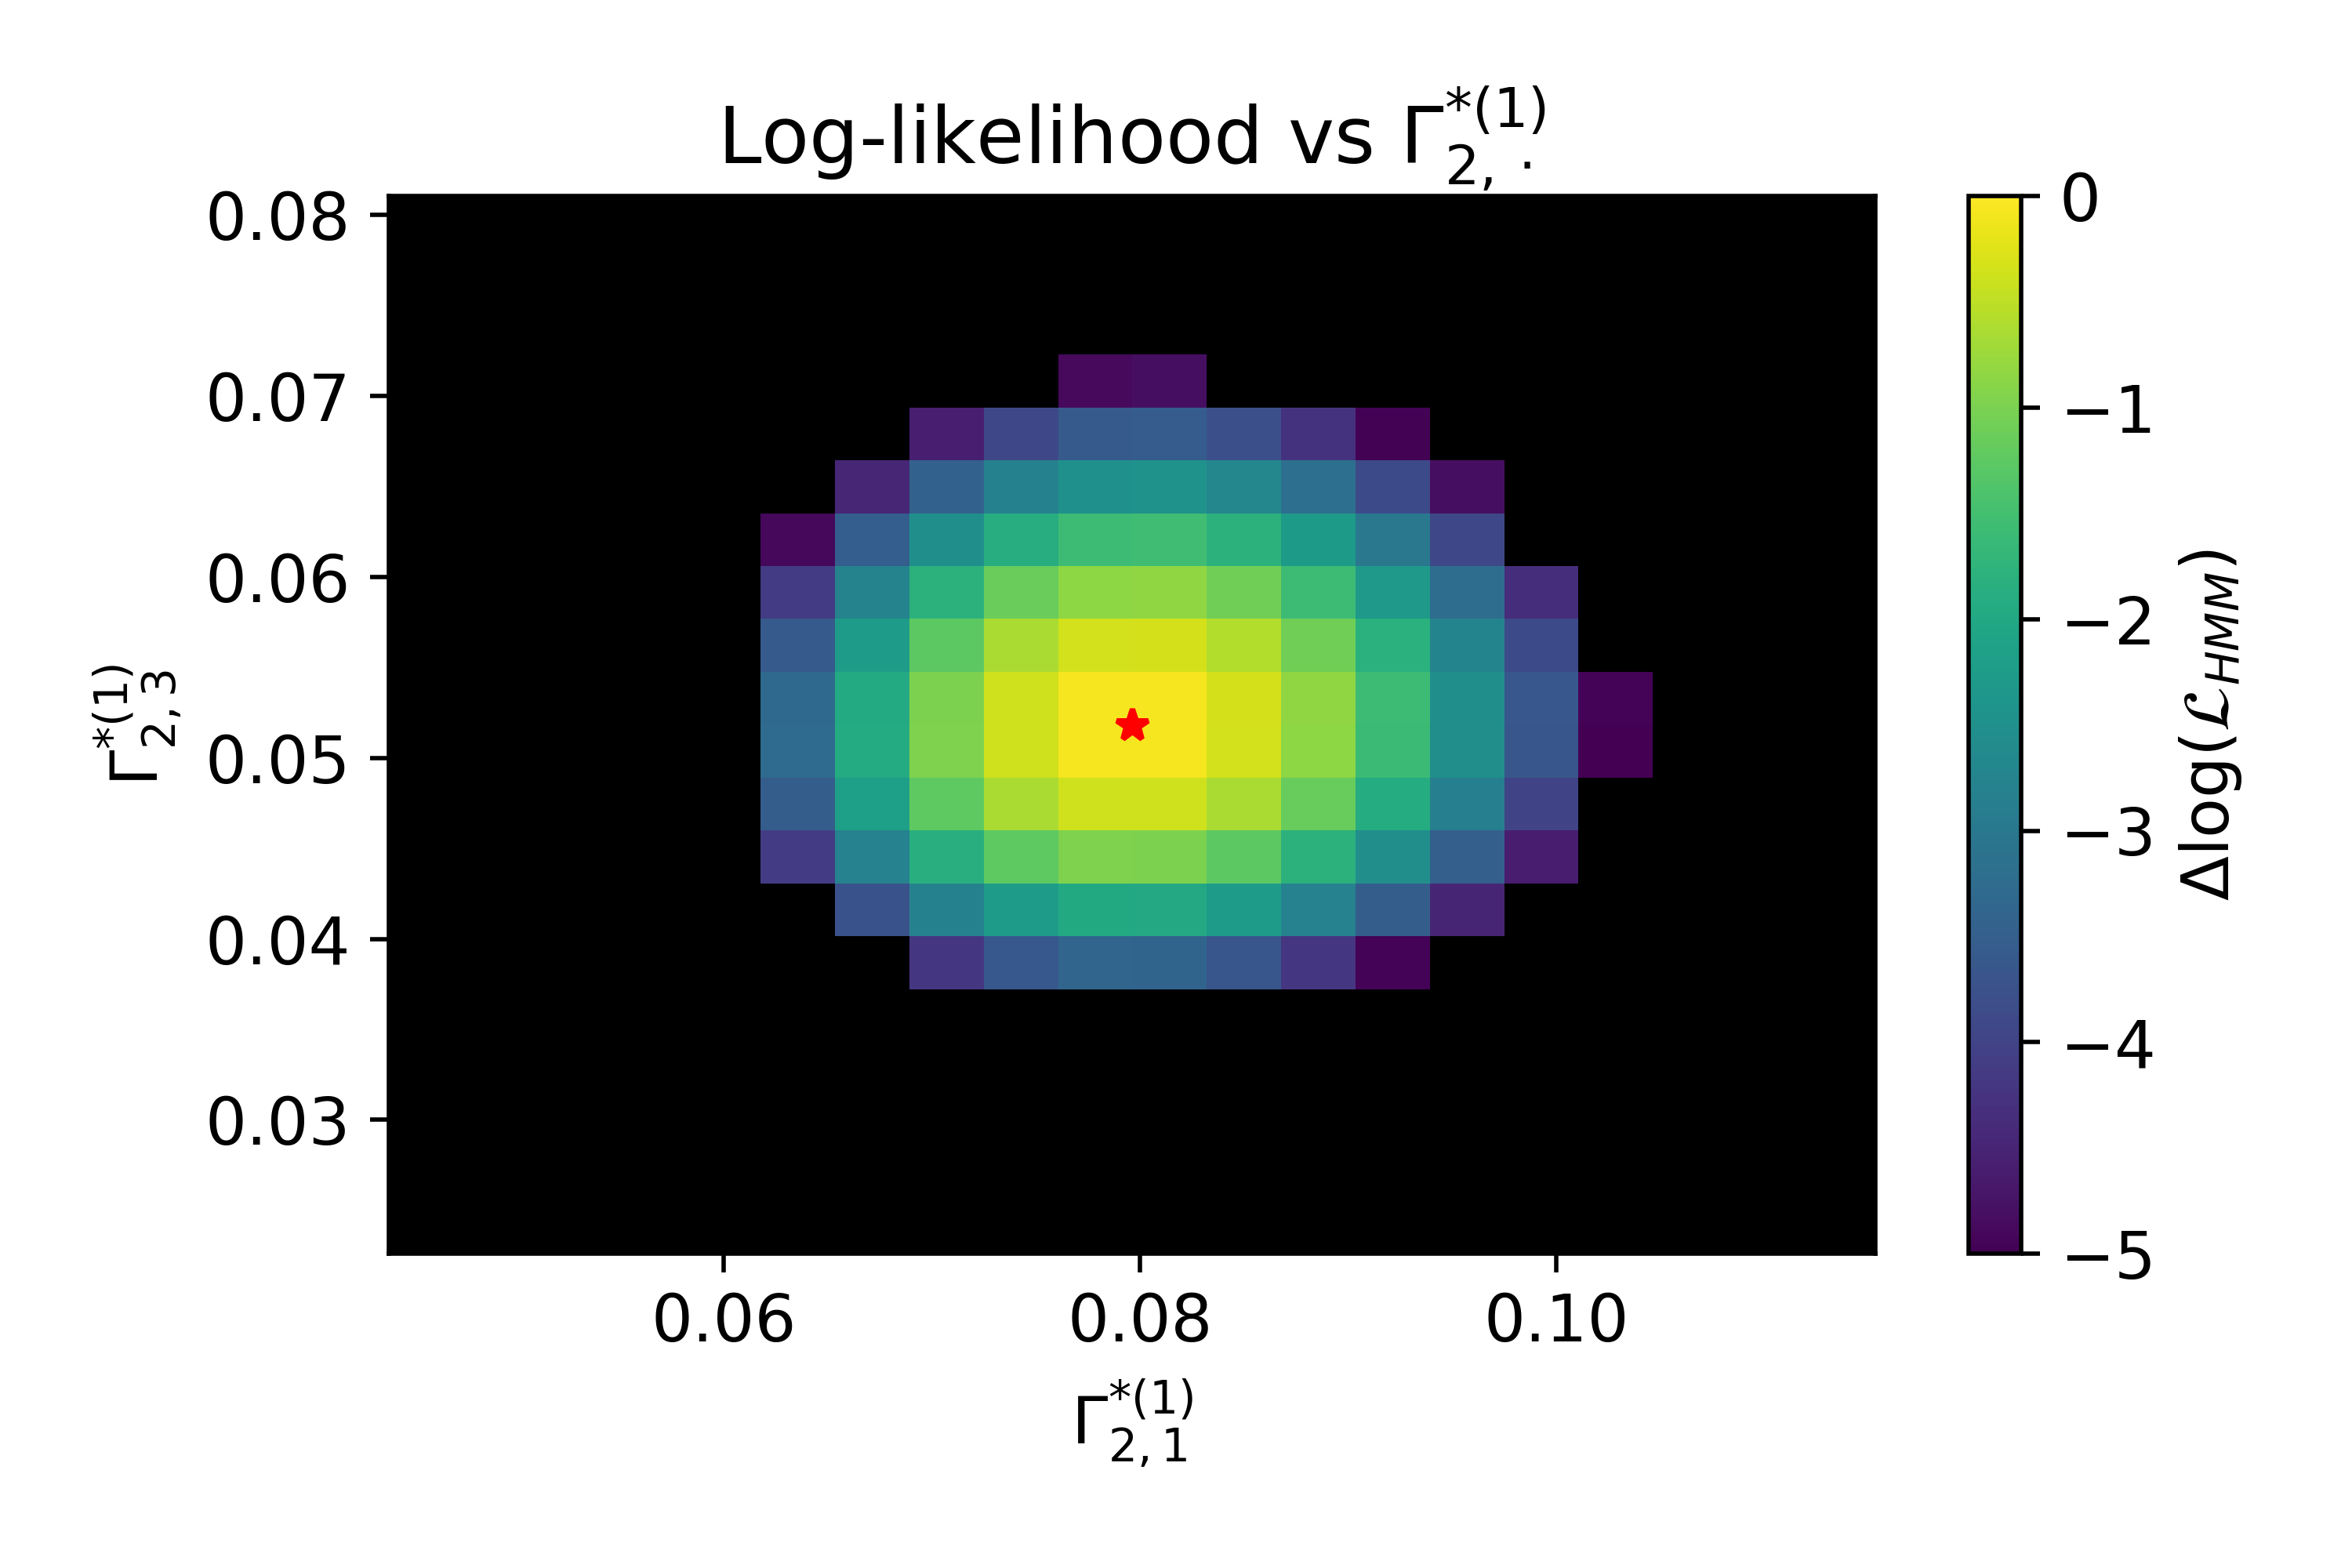
\includegraphics[width=3in]{../Plots/2019/20190902-182840-CATs_OB_1_0_267_CarHHMM2_fine-gamma-likelihood-0-row_1.png}
        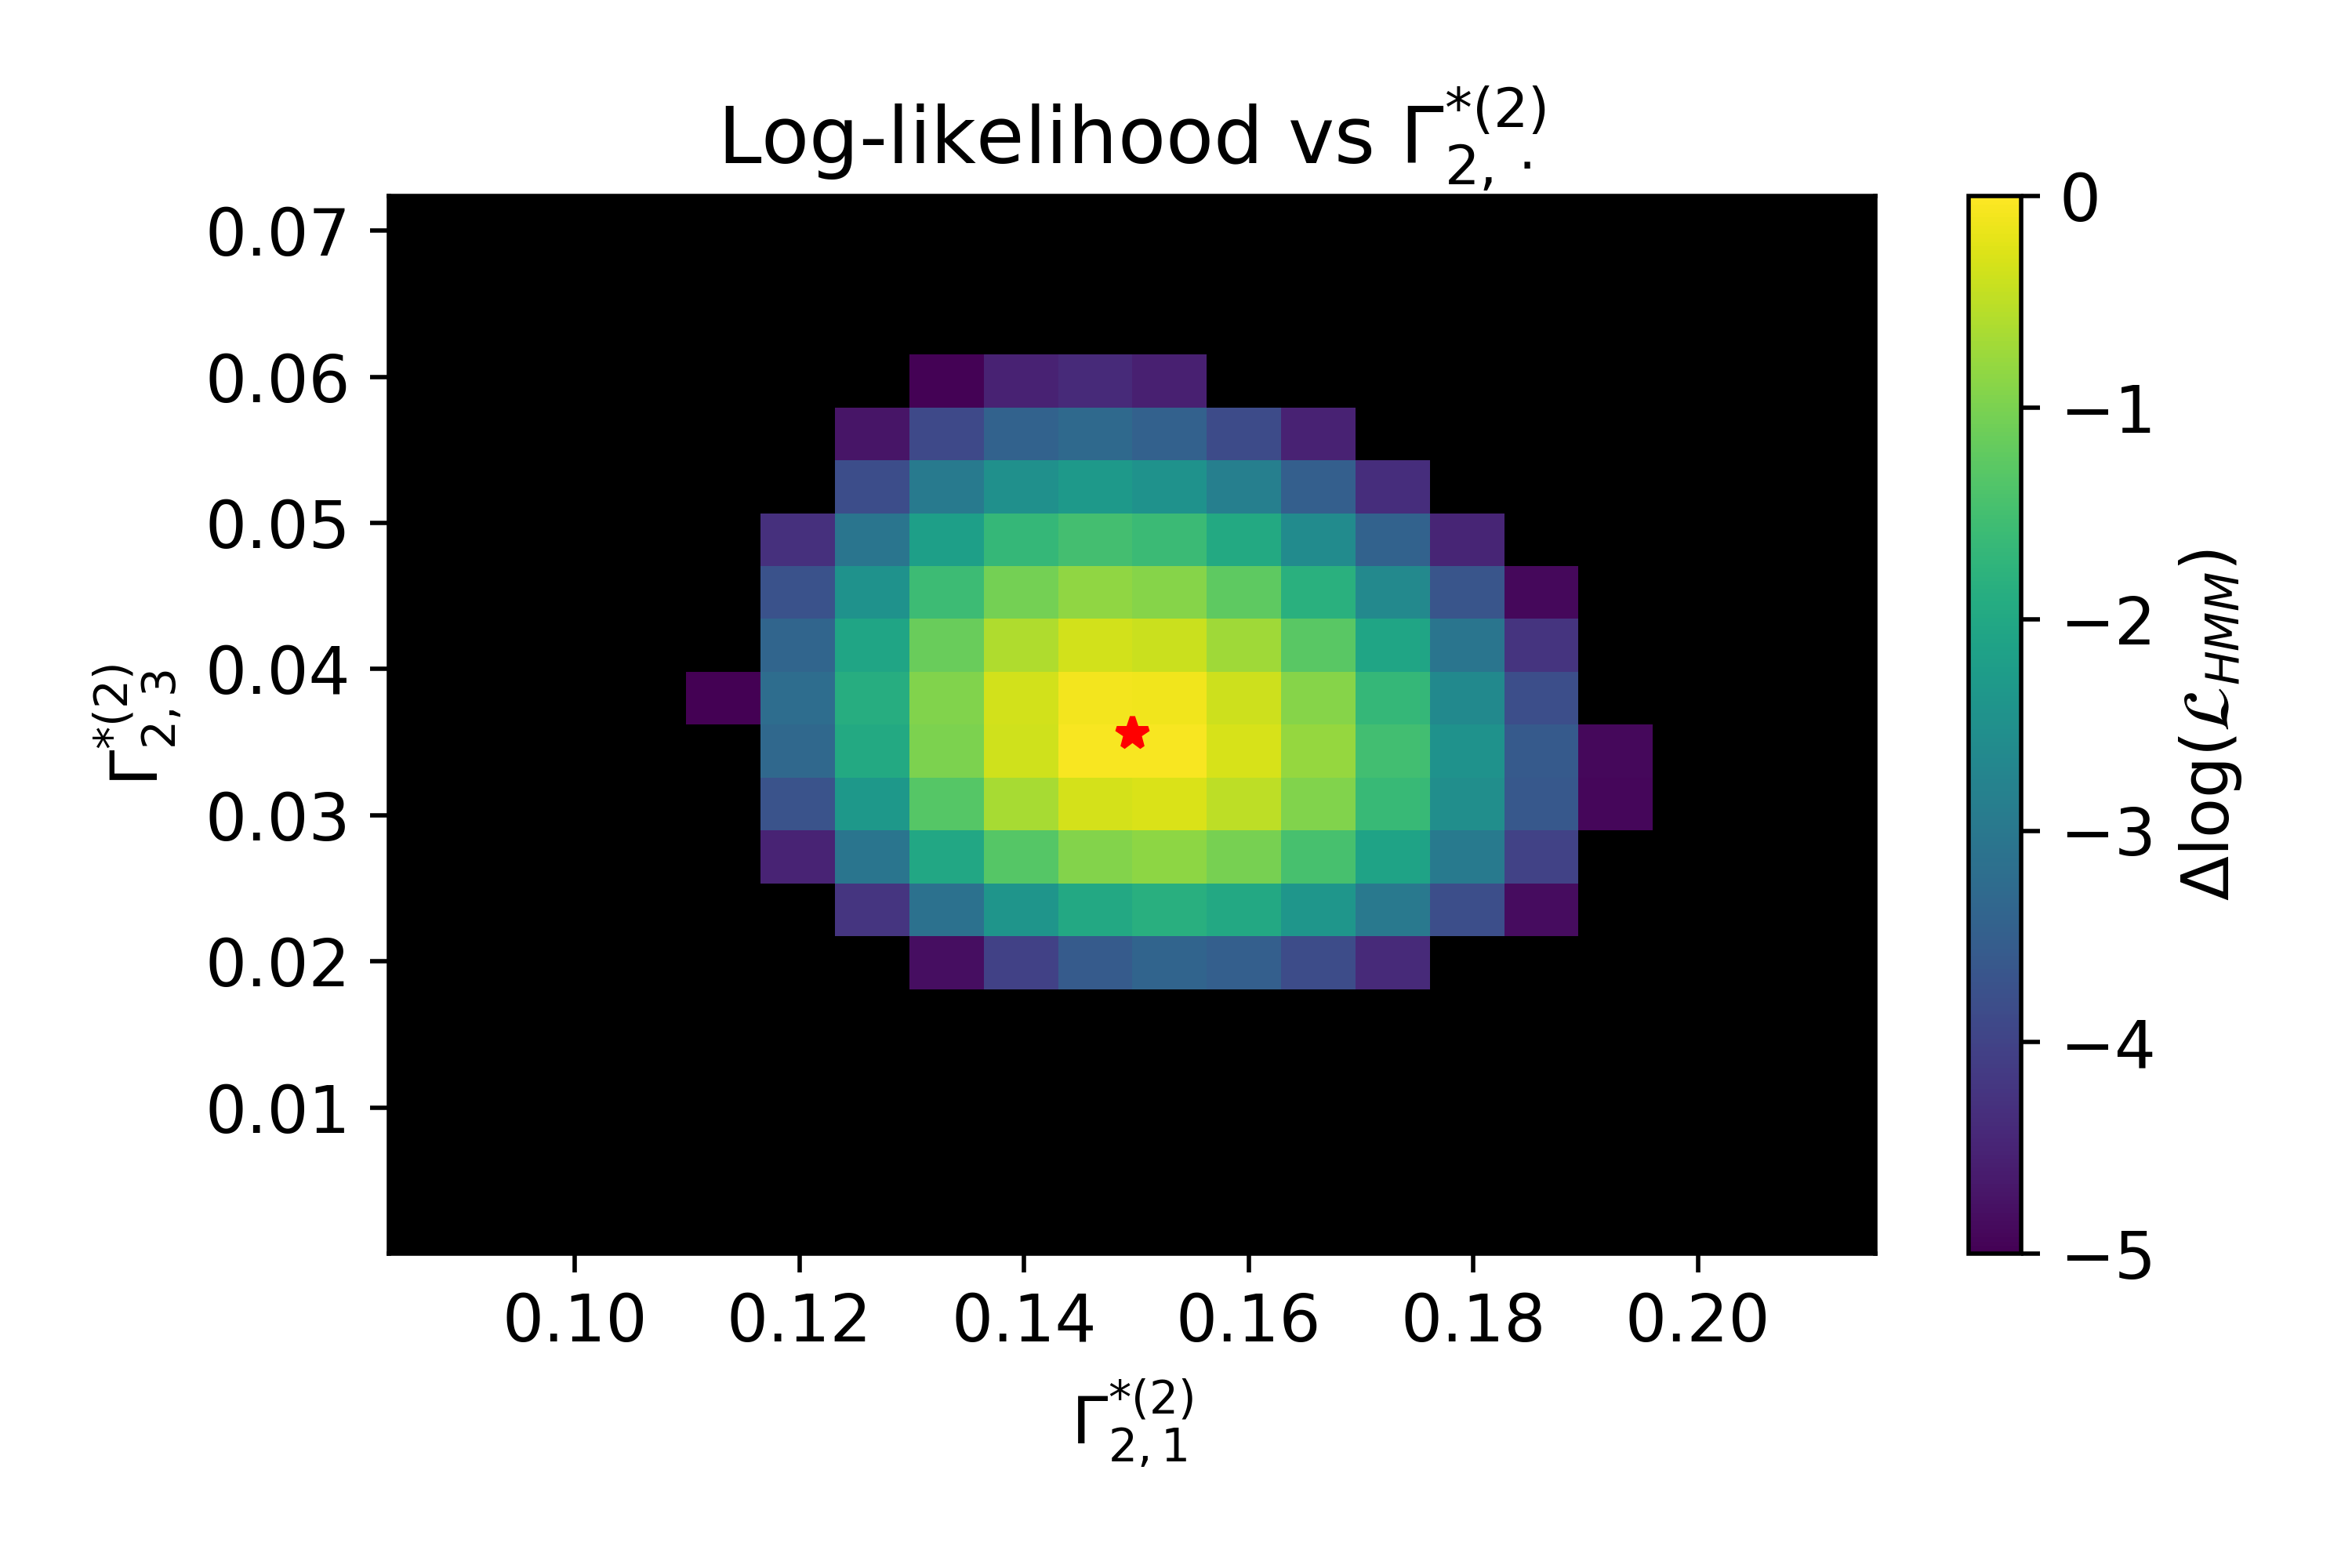
\includegraphics[width=3in]{../Plots/2019/20190902-182840-CATs_OB_1_0_267_CarHHMM2_fine-gamma-likelihood-1-row_1.png}
        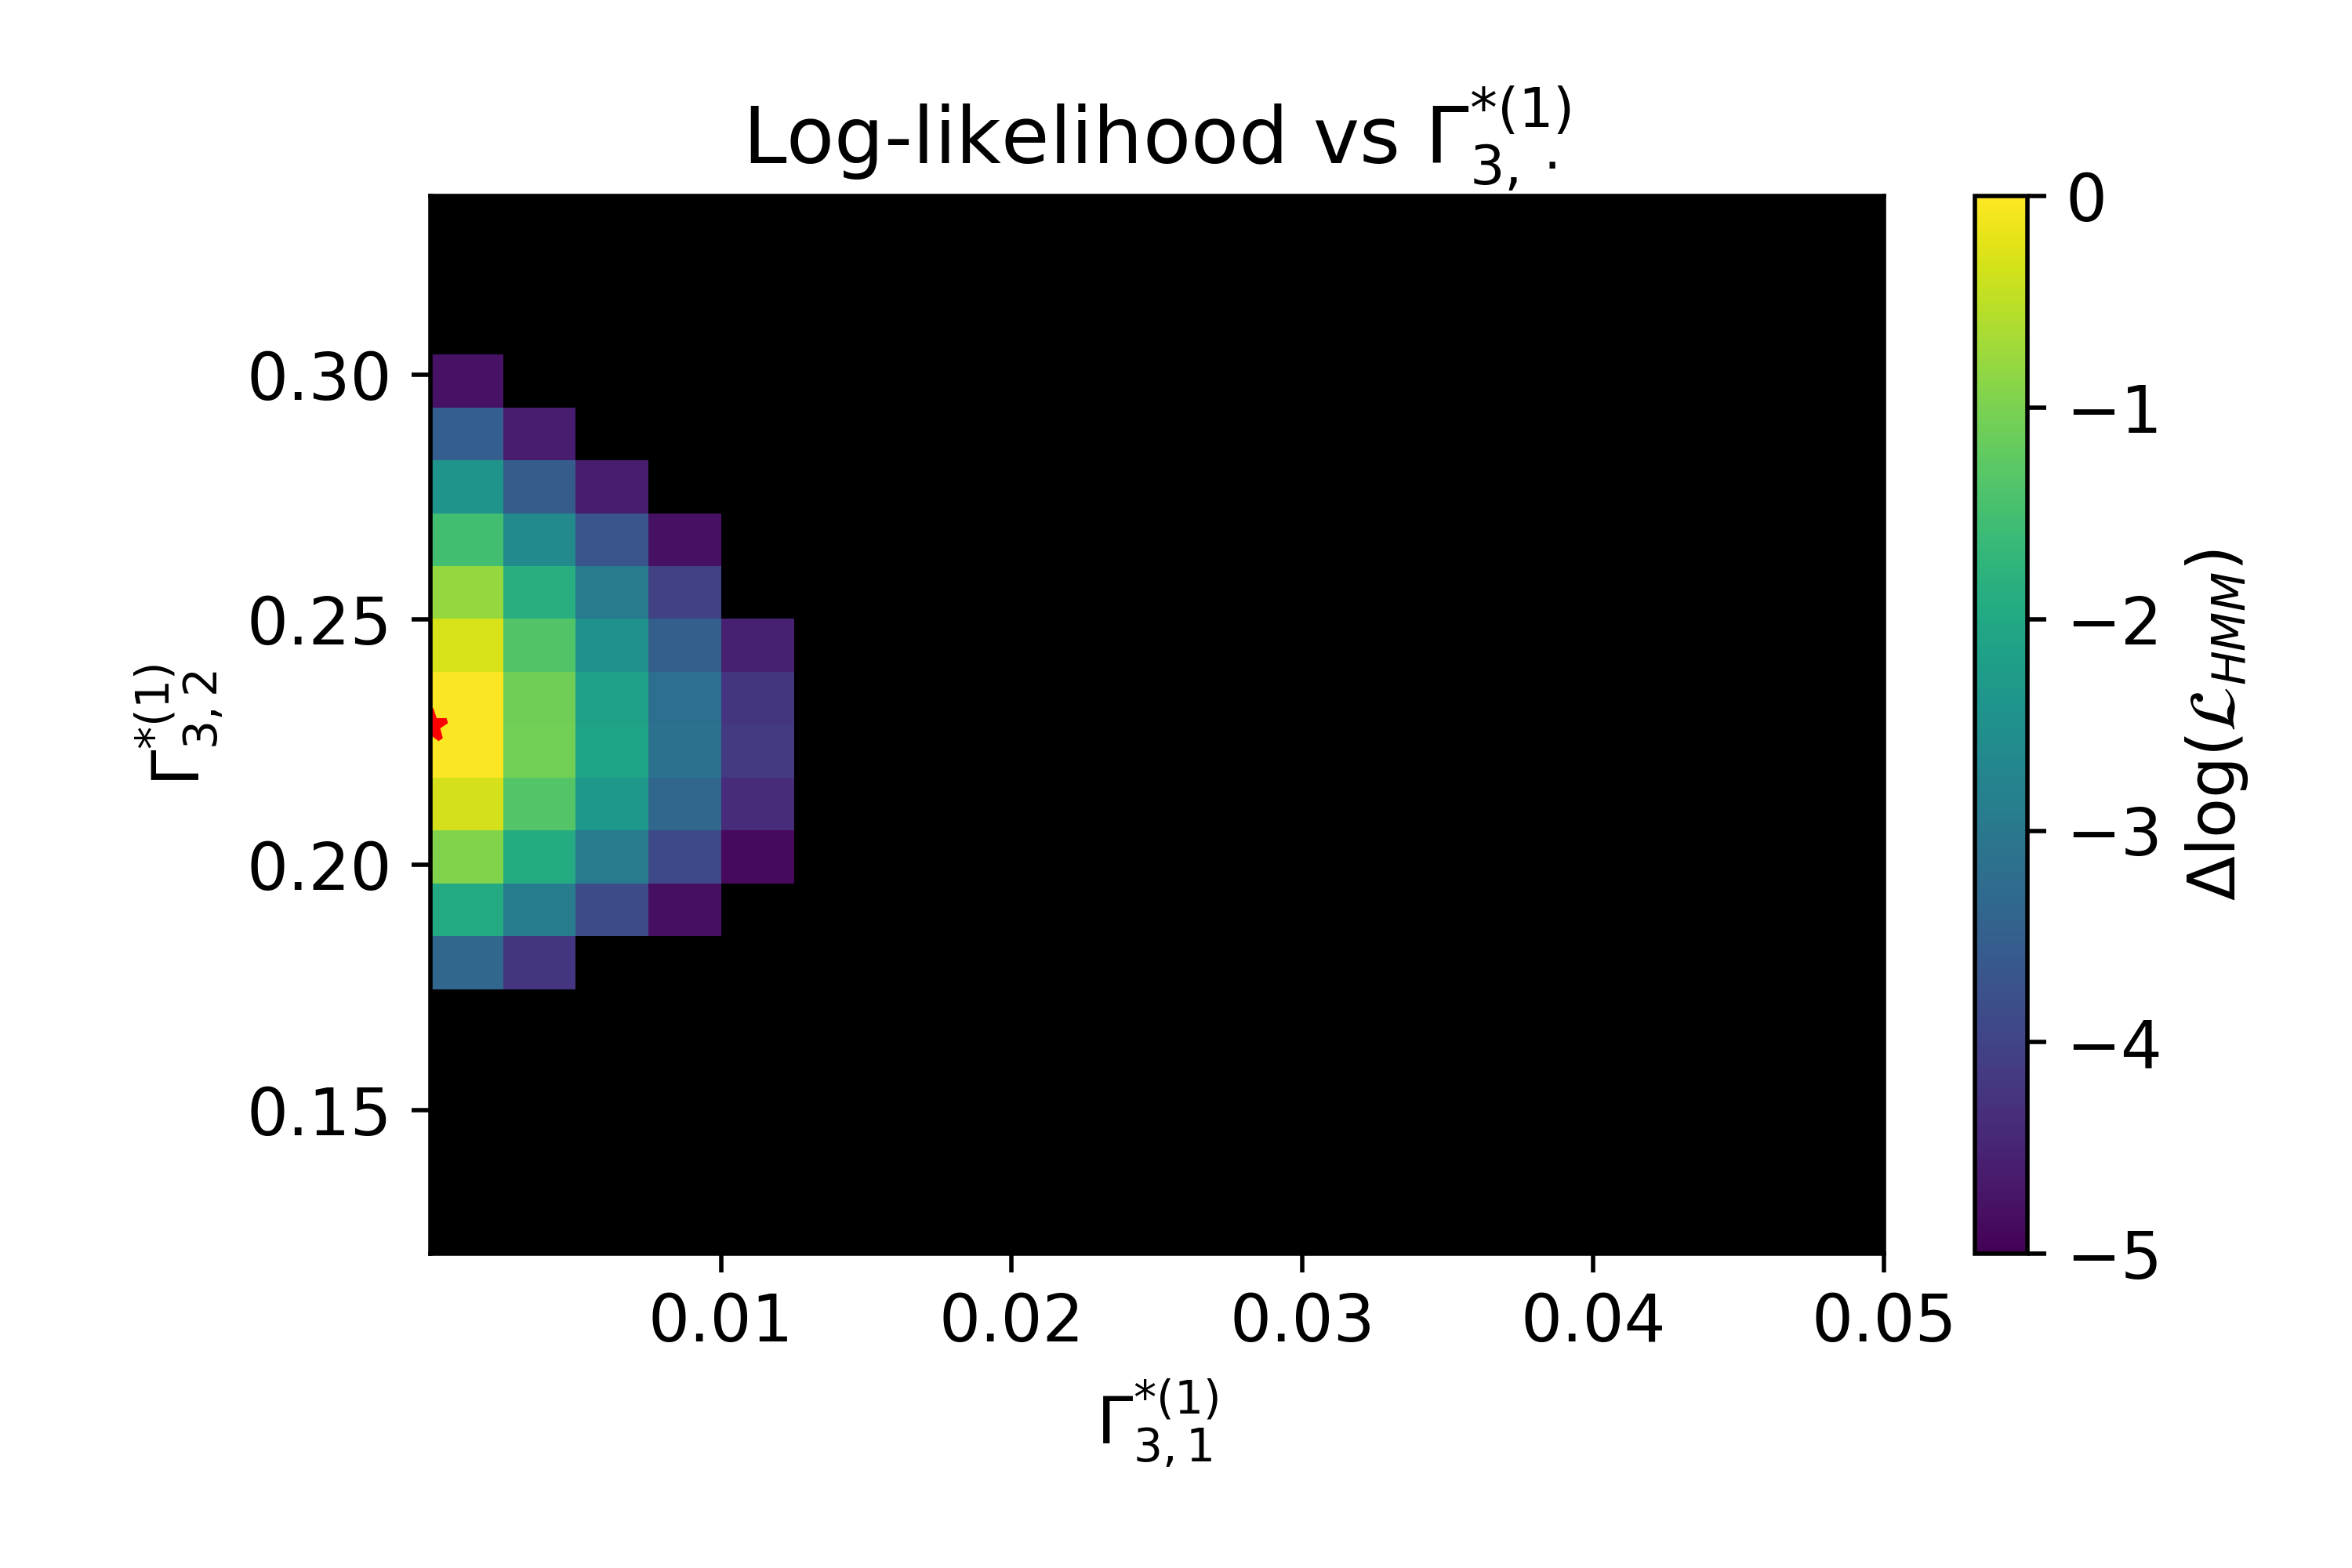
\includegraphics[width=3in]{../Plots/2019/20190902-182840-CATs_OB_1_0_267_CarHHMM2_fine-gamma-likelihood-0-row_2.png}
        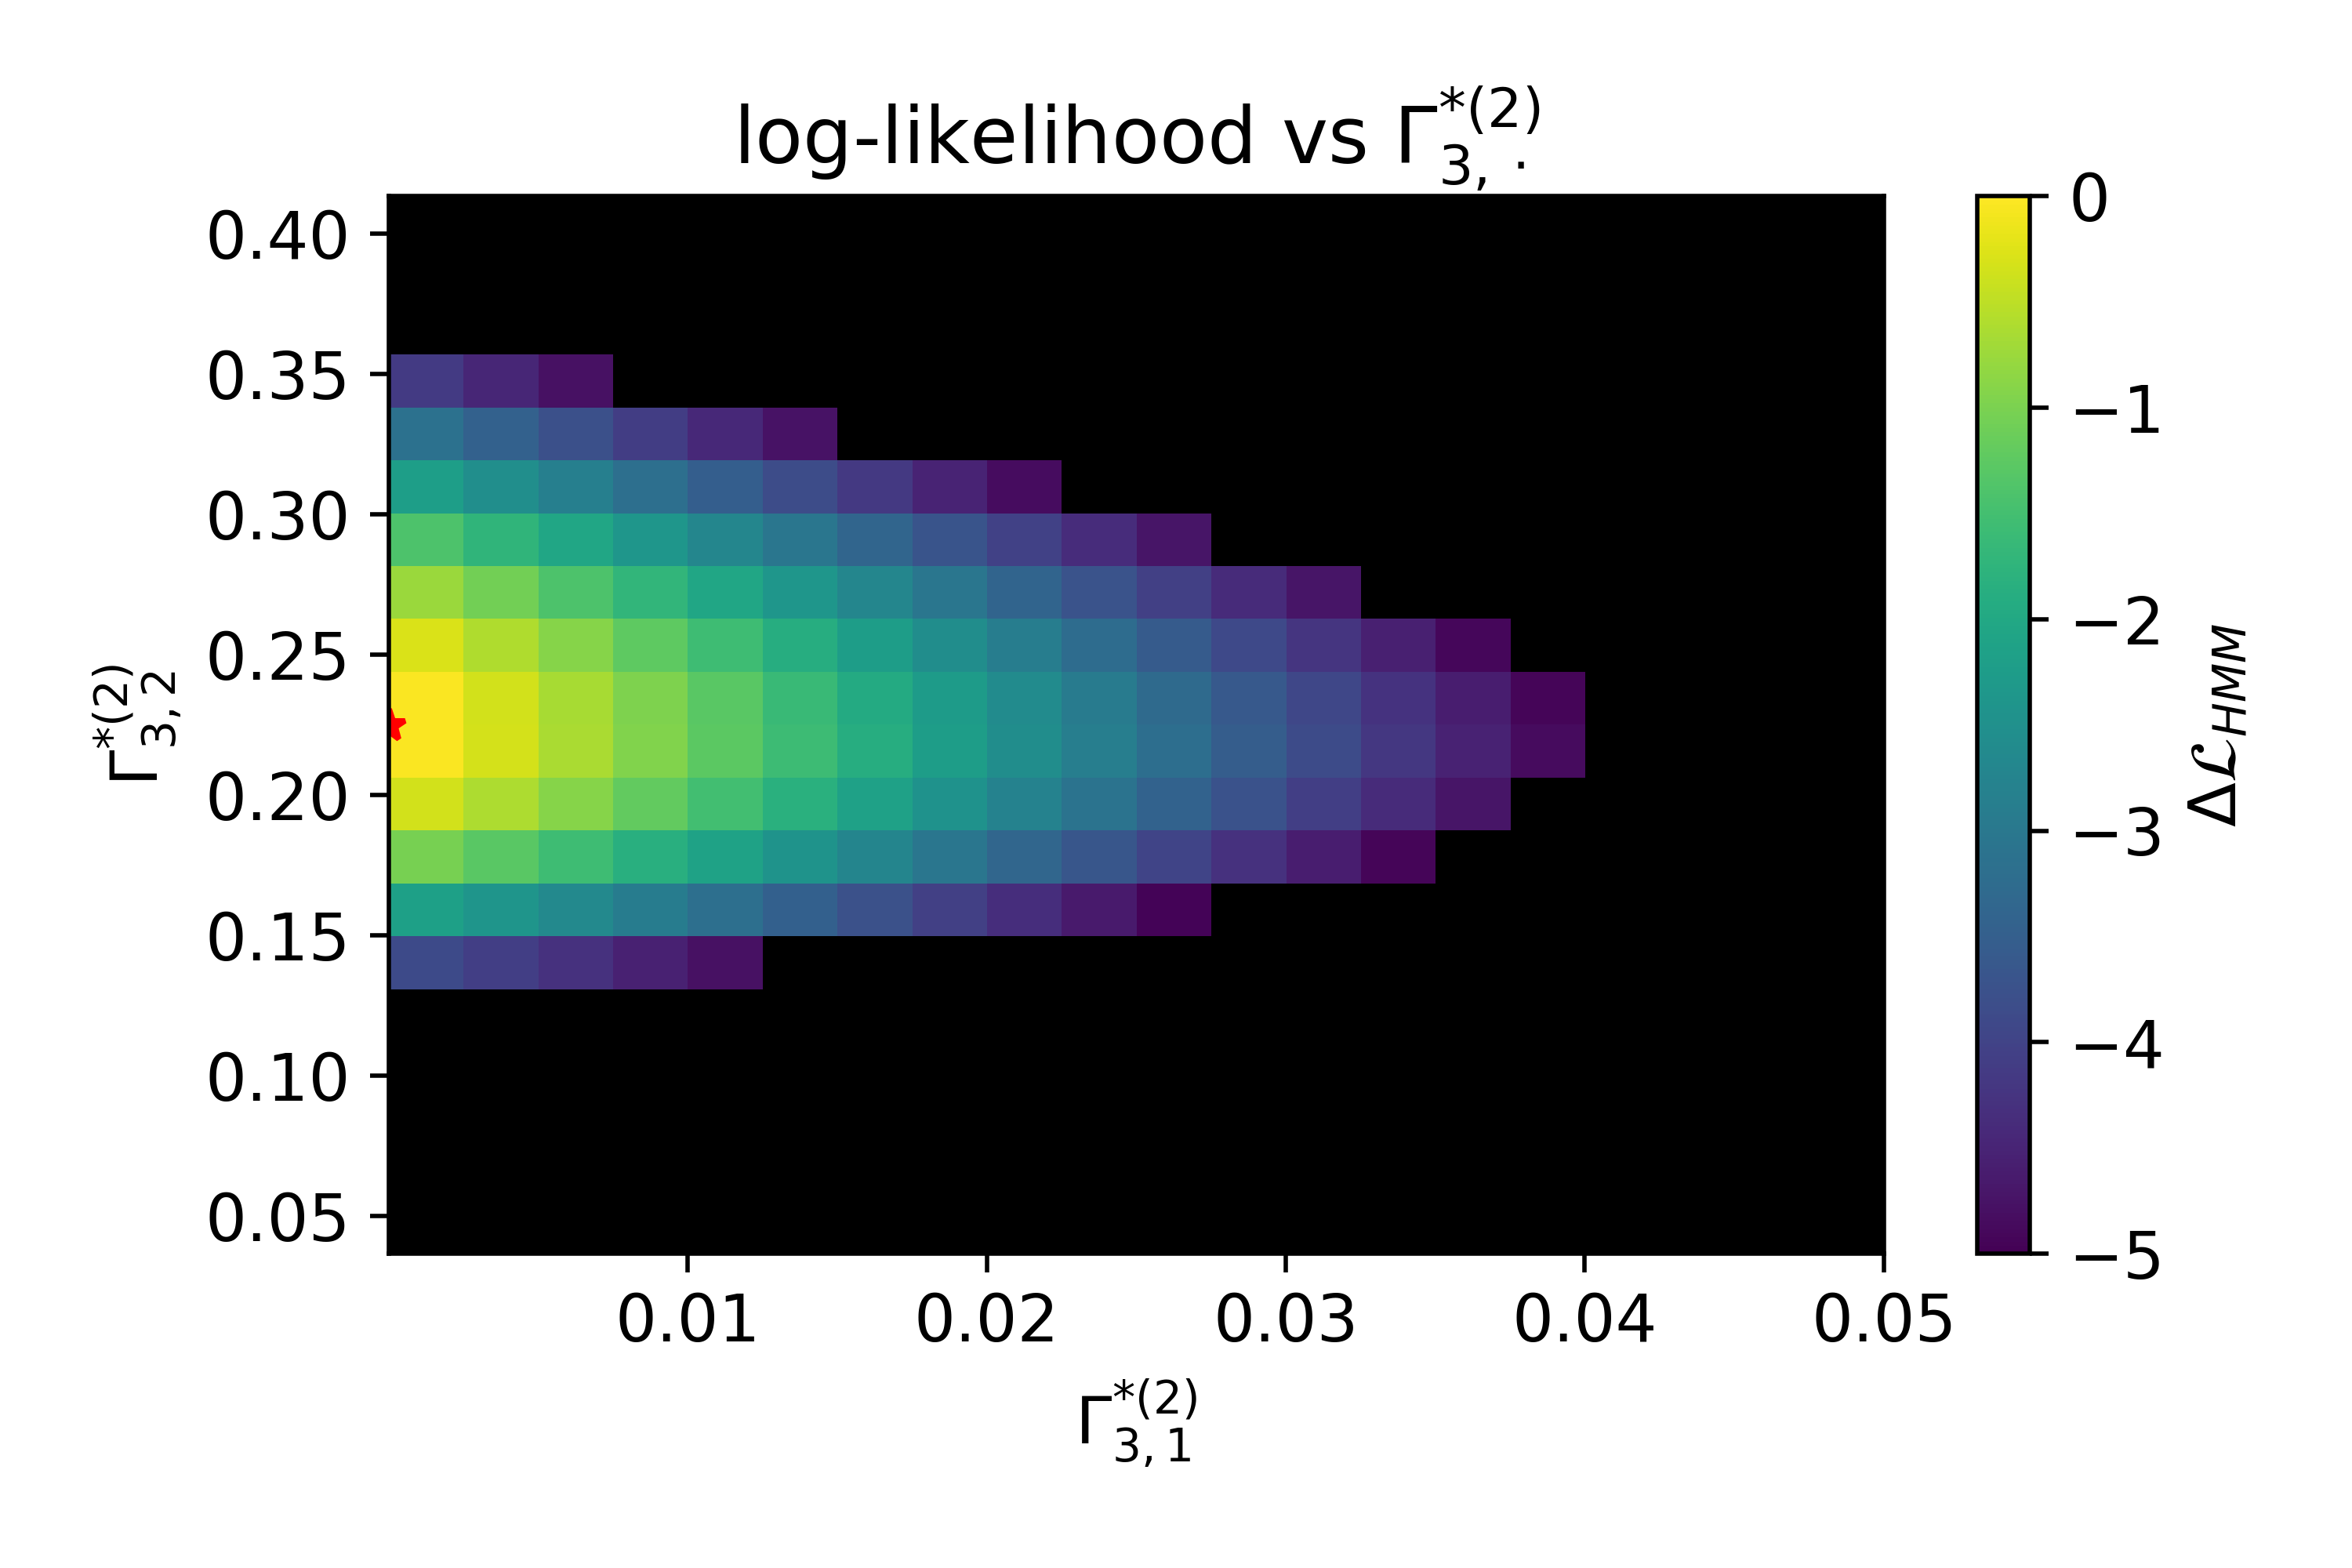
\includegraphics[width=3in]{../Plots/2019/20190902-182840-CATs_OB_1_0_267_CarHHMM2_fine-gamma-likelihood-1-row_2.png}
        \end{center}
        
        \noindent Figure \arabic{fignum}: Log-likelihood of the CarHHMM-DFT as a function of the fine-scale probability transition matrix parameters associated both dive types ($\Gamma^{*(i)}_{i^*,j^*}$ for dive types $i = 1,2$ and subdive states $i^*,j^* = 1,2,3$). All other parameters and probability transition matrices are set to be equal to the maximum likelihood estimates shown in Table (1) of Section 3.1. The log-likelihood is added to the negative log-likelihood of the maximum likelihood estimate $\hat \Gamma^{*(i)}$, which is denoted by a red star. Note that $\hat \Gamma^{*(i)}_{1,3} \approx \hat \Gamma^{*(i)}_{3,1} \approx 0$. This indicates that the whale rarely switches directly between subdive states 1 and 3.
        \addtocounter{fignum}{1}
        
        \newpage    
    
    \section{Parameter Estimates}

        \subsection{CarHHMM-DFT}
        
            %\begin{table}[ht]
            %
            %\caption{Estimates and empirical standard errors of emission parameters for dive duration ($Y_t$), acceleration ($\Zone_{t,\tilde t^*}$), and wiggliness ($\Ztwo_{t,\tilde t^*}$) of the killer whale case study data under the full CarHHMM-DFT.}
            \begin{center}
            \scalebox{0.75}{
            \bgroup
            \centering
            \def\arraystretch{1.5}
            \begin{tabular}{ccccc}
                \multirow{2}{*}{Feature}                                                       & \multirow{2}{*}{Dive / Subdive Type} & \multicolumn{3}{c}{Parameter Estimate}        \\
                                                                                               &                                      & $\hat \mu$    & $\hat \sigma$ & $\hat \phi$   \\ \hline
                \multirow{2}{*}{Dive Duration $(s)$ -- $Y_t$}                                  & 1                                    & $27.34 (0.63)$ & $10.96 (0.56)$ & ---           \\
                                                                                               & 2                                    & $127.5 (11.3)$ & $63.9 (9.0)$ & ---           \\ \hline
                \multirow{3}{*}{$x$-Acc. $(m/s^2)$ -- $\left(\Zone_{t,\tilde t^*}\right)_x$}   & 1                                    & $0.449 (0.030)$ & $0.039 (0.001)$ & $0.968 (0.002)$ \\
                                                                                               & 2                                    & $0.210 (0.012)$ & $0.096 (0.002)$ & $0.829 (0.007)$ \\
                                                                                               & 3                                    & $0.232 (0.035)$ & $0.296 (0.010)$ & $0.607 (0.023)$ \\ \hline
                \multirow{3}{*}{$y$-Acc. $(m/s^2)$ -- $\left(\Zone_{t,\tilde t^*}\right)_y$}   & 1                                    & $0.450 (0.038)$ & $0.051 (0.001)$ & $0.968 (0.002)$ \\
                                                                                               & 2                                    & $0.437 (0.012)$ & $0.094 (0.002)$ & $0.829 (0.007)$ \\
                                                                                               & 3                                    & $0.366 (0.042)$ & $0.365 (0.012)$ & $0.607 (0.023)$ \\ \hline
                \multirow{3}{*}{$z$-Acc. $(m/s^2)$ -- $\left(\Zone_{t,\tilde t^*}\right)_z$}   & 1                                    & $-0.691 (0.043)$ & $0.058 (0.001)$ & $0.968 (0.002)$ \\
                                                                                               & 2                                    & $-0.573 (0.014)$ & $0.111 (0.002)$ & $0.829 (0.007)$ \\
                                                                                               & 3                                    & $-0.303 (0.041)$ & $0.354 (0.012)$ & $0.607 (0.023)$ \\ \hline
                \multirow{3}{*}{Wiggliness - $\Ztwo_{t,\tilde t^*}$}                           & 1                                    & $34.02 (0.36)$ & $22.99 (0.38)$ & ---           \\
                                                                                               & 2                                    & $490.1 (5.6)$ & $502.6 (6.8)$ & ---           \\
                                                                                               & 3                                    & $9150 (220)$ & $13540 (350)$ & ---           \\ \hline
            \end{tabular}
            \egroup
            }
            \end{center}
            
            \noindent Table \arabic{tablenum}: Estimates and predicted standard errors of emission parameters for dive duration ($Y_t$), acceleration ($\Zone_{t,\tilde t^*}$), and wiggliness ($\Ztwo_{t,\tilde t^*}$) of the killer whale case study data under the full CarHHMM-DFT. The parentheses refer to the estimated standard error of the parameter estimates derived from the inverse of the observed information matrix.
            \addtocounter{tablenum}{1}
    
        \subsection{HHMM-DFT}
        
            \begin{center}
            \scalebox{0.75}{
                \bgroup
                \centering
                \def\arraystretch{1.5}
                \begin{tabular}{ccccc}
                \multirow{2}{*}{Feature}                                                       & \multirow{2}{*}{Dive / Subdive Type} & \multicolumn{3}{c}{Parameter Estimate}          \\
                                                                                               &                                      & $\hat \mu$    & $\hat \sigma$ & $\hat \phi$     \\ \hline
                \multirow{2}{*}{Dive Duration $(s)$ -- $Y_t$}                                  & 1                                    & $26.61 (0.61)$ & $10.16 (0.52)$ & ---             \\
                                                                                               & 2                                    & $116.8 (10.6)$ & $64.7 (8.6)$ & ---             \\ \hline
                \multirow{3}{*}{$x$-Acc. $(m/s^2)$ -- $\left(\Zone_{t,\tilde t^*}\right)_x$}   & 1                                    & $0.000 (0.002)$ & $0.065 (0.001)$ & ---             \\
                                                                                               & 2                                    & $0.085 (0.004)$ & $0.175 (0.003)$ & ---             \\
                                                                                               & 3                                    & $0.291 (0.020)$ & $0.484 (0.014)$ & ---             \\ \hline
                \multirow{3}{*}{$y$-Acc. $(m/s^2)$ -- $\left(\Zone_{t,\tilde t^*}\right)_y$}   & 1                                    & $0.365 (0.002)$ & $0.068 (0.001)$ & ---             \\
                                                                                               & 2                                    & $0.408 (0.002)$ & $0.108 (0.002)$ & ---             \\
                                                                                               & 3                                    & $0.275 (0.017)$ & $0.407 (0.012)$ & ---             \\ \hline
                \multirow{3}{*}{$z$-Acc. $(m/s^2)$ -- $\left(\Zone_{t,\tilde t^*}\right)_z$}   & 1                                    & $-0.442 (0.003)$ & $0.101 (0.002)$ & ---             \\
                                                                                               & 2                                    & $-0.471 (0.003)$ & $0.158 (0.002)$ & ---             \\
                                                                                               & 3                                    & $-0.298 (0.017)$ & $0.415 (0.012)$ & ---             \\ \hline
                \multirow{3}{*}{Wiggliness - $\Ztwo_{t,\tilde t^*}$}                           & 1                                    & $43.65 (0.52)$ & $33.66 (0.58)$ & ---             \\
                                                                                               & 2                                    & $608.0 (6.8)$ & $717.3 (9.2)$ & ---             \\
                                                                                               & 3                                    & $7100 (160)$ & $13620 (310)$ & ---             \\ \hline
                \end{tabular}
                \egroup
            }
            \end{center}
            
            \noindent Table \arabic{tablenum}: Estimates and predicted standard errors of emission parameters for dive duration ($Y_t$), acceleration ($\Zone_{t,\tilde t^*}$), and wiggliness ($\Ztwo_{t,\tilde t^*}$) of the killer whale case study data under the HHMM-DFT. The parentheses refer to the estimated standard error of the parameter estimates derived from the inverse of the observed information matrix.
            \addtocounter{tablenum}{1}
            
        \subsection{CarHHMM}
            
            \begin{center}
            \scalebox{0.75}{
                \bgroup
                \centering
                \def\arraystretch{1.5}
                \begin{tabular}{ccccc}
                \multirow{2}{*}{Feature}                                                       & \multirow{2}{*}{Dive / Subdive Type} & \multicolumn{3}{c}{Parameter Estimate}        \\
                                                                                               &                                      & $\hat \mu$    & $\hat \sigma$ & $\hat \phi$   \\ \hline
                \multirow{2}{*}{Dive Duration $(s)$ -- $Y_t$}                                  & 1                                    & $27.16 (0.63)$ & $10.78 (0.55)$ & ---           \\
                                                                                               & 2                                    & $124.2 (11.0)$ & $64.6 (8.8)$ & ---           \\ \hline
                \multirow{3}{*}{$x$-Acc. $(m/s^2)$ -- $\left(\Zone_{t,\tilde t^*}\right)_x$}   & 1                                    & $0.064 (0.007)$ & $0.035 (0.001)$ & $0.874 (0.008)$ \\
                                                                                               & 2                                    & $0.342 (0.017)$ & $0.095 (0.002)$ & $0.879 (0.005)$ \\
                                                                                               & 3                                    & $0.257 (0.037)$ & $0.305 (0.010)$ & $0.605 (0.023)$ \\ \hline
                \multirow{3}{*}{$y$-Acc. $(m/s^2)$ -- $\left(\Zone_{t,\tilde t^*}\right)_y$}   & 1                                    & $0.376 (0.009)$ & $0.044 (0.001)$ & $0.874 (0.008)$ \\
                                                                                               & 2                                    & $0.470 (0.017)$ & $0.097 (0.002)$ & $0.879 (0.005)$ \\
                                                                                               & 3                                    & $0.350 (0.045)$ & $0.377 (0.013)$ & $0.605 (0.023)$ \\ \hline
                \multirow{3}{*}{$z$-Acc. $(m/s^2)$ -- $\left(\Zone_{t,\tilde t^*}\right)_z$}   & 1                                    & $-0.462 (0.011)$ & $0.052 (0.001)$ & $0.874 (0.008)$ \\
                                                                                               & 2                                    & $-0.660 (0.020)$ & $0.113 (0.002)$ & $0.879 (0.005)$ \\
                                                                                               & 3                                    & $-0.306 (0.045)$ & $0.369 (0.013)$ & $0.605 (0.023)$ \\ \hline
                \end{tabular}
                \egroup
            }
            \end{center}
            
                \noindent Table \arabic{tablenum}: Estimates and predicted standard errors of emission parameters for dive duration ($Y_t$) and acceleration ($\Zone_{t,\tilde t^*}$) of the killer whale case study data under the CarHHMM. The parentheses refer to the estimated standard error of the parameter estimates derived from the inverse of the observed information matrix.
                \addtocounter{tablenum}{1}
            
        \subsection{CarHMM-DFT}
        
            \begin{center}
            \scalebox{0.75}{
                \bgroup
                \centering
                \def\arraystretch{1.5}
            \begin{tabular}{ccccc}
            \multirow{2}{*}{Feature}                                                       & \multirow{2}{*}{Dive / Subdive Type} & \multicolumn{3}{c}{Parameter Estimate}        \\
                                                                                           &                                      & $\hat \mu$    & $\hat \sigma$ & $\hat \phi$   \\ \hline
            \multirow{1}{*}{Dive Duration $(s)$ -- $Y_t$}                                  & 1                                    & $41.70 (1.24)$ & $30.50 (1.22)$ & ---           \\ \hline
            \multirow{3}{*}{$x$-Acc. $(m/s^2)$ -- $\left(\Zone_{t,\tilde t^*}\right)_x$}   & 1                                    & $0.460 (0.030)$ & $0.039 (0.001)$ & $0.968 (0.002)$ \\
                                                                                           & 2                                    & $0.209 (0.012)$ & $0.096 (0.002)$ & $0.828 (0.007)$ \\
                                                                                           & 3                                    & $0.232 (0.035)$ & $0.296 (0.010)$ & $0.607 (0.023)$ \\ \hline
            \multirow{3}{*}{$y$-Acc. $(m/s^2)$ -- $\left(\Zone_{t,\tilde t^*}\right)_y$}   & 1                                    & $0.457 (0.038)$ & $0.052 (0.001)$ & $0.968 (0.002)$ \\
                                                                                           & 2                                    & $0.436 (0.012)$ & $0.094 (0.002)$ & $0.828 (0.007)$ \\
                                                                                           & 3                                    & $0.365 (0.042)$ & $0.366 (0.012)$ & $0.607 (0.023)$ \\ \hline
            \multirow{3}{*}{$z$-Acc. $(m/s^2)$ -- $\left(\Zone_{t,\tilde t^*}\right)_z$}   & 1                                    & $-0.704 (0.044)$ & $0.059 (0.001)$ & $0.968 (0.002)$ \\
                                                                                           & 2                                    & $-0.571 (0.014)$ & $0.111 (0.002)$ & $0.828 (0.007)$ \\
                                                                                           & 3                                    & $-0.301 (0.042)$ & $0.355 (0.012)$ & $0.607 (0.023)$ \\ \hline
            \multirow{3}{*}{Wiggliness - $\Ztwo_{t,\tilde t^*}$}                           & 1                                    & $34.40 (0.37)$ & $23.33 (0.38)$ & ---           \\
                                                                                           & 2                                    & $495.0 (5.7)$ & $505.4 (6.9)$ & ---           \\
                                                                                           & 3                                    & $9190 (220)$ & $13590 (360)$ & ---           \\ \hline
            \end{tabular}
                \egroup
            }
            \end{center}
            
                \noindent Table \arabic{tablenum}: Estimates and predicted standard errors of emission parameters for dive duration ($Y_t$), acceleration ($\Zone_{t,\tilde t^*}$), and wiggliness ($\Ztwo_{t,\tilde t^*}$) of the killer whale case study data under the CarHMM-DFT. The parentheses refer to the estimated standard error of the parameter estimates derived from the inverse of the observed information matrix.
                \addtocounter{tablenum}{1}
    
    \newpage
    \section{Decoded dive states}
    
        \subsection{CarHHMM-DFT}
        
        \begin{center}
        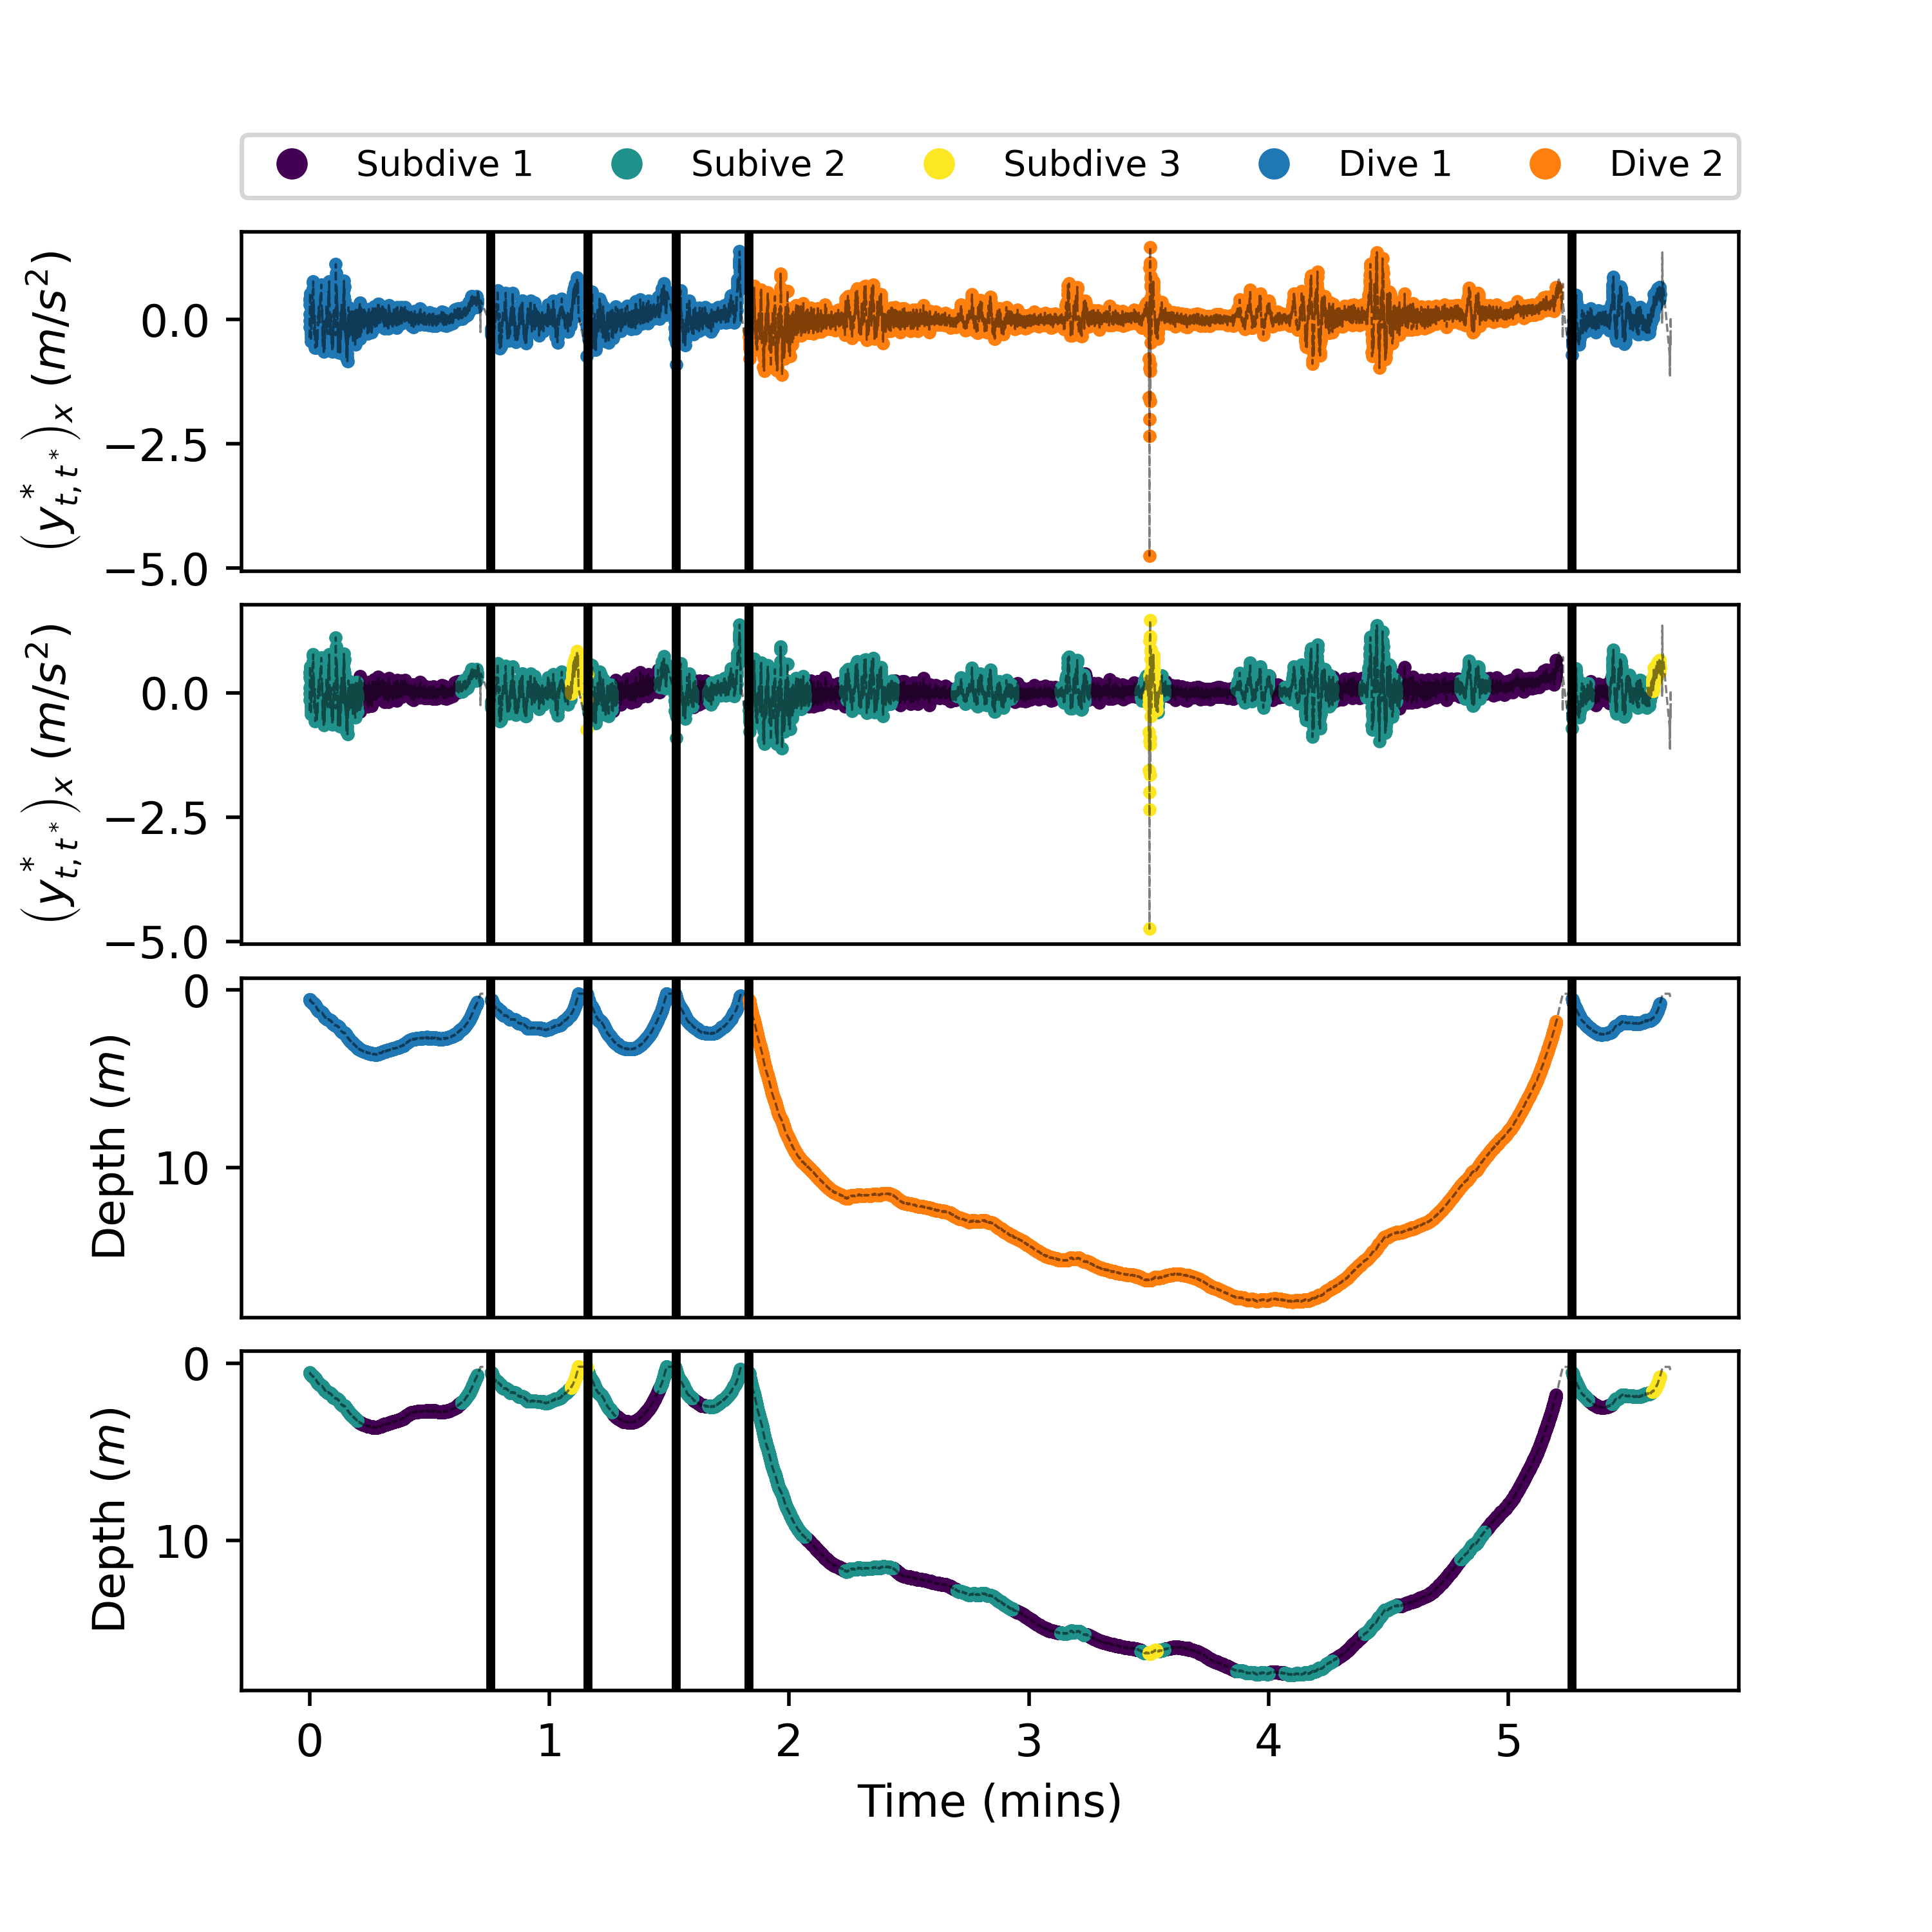
\includegraphics[width=6in]{../Plots/2019/20190902-182840-CATs_OB_1_0_267_CarHHMM2_decoded_dives.png}
        \end{center}
        
        \noindent Figure \arabic{fignum}: The $x$--component of acceleration $(y^*_{t,t^*})_x$ (top two panels) and dive depth (bottom two panels) of a northern resident killer whale for a sequence of six selected dives. Each panel is partitioned into dives by vertical black lines. The curve colours in the first and third panels correspond to the estimated dive types while the curve colours of the second and fourth panels correspond the estimated subdive states. Both the dive types and subdive states are estimated by fitting the CarHHMM-DFT to the data and performing the forward-backward algorithm to determine the hidden state with the highest probability.
        \addtocounter{fignum}{1}
        
        \begin{center}
        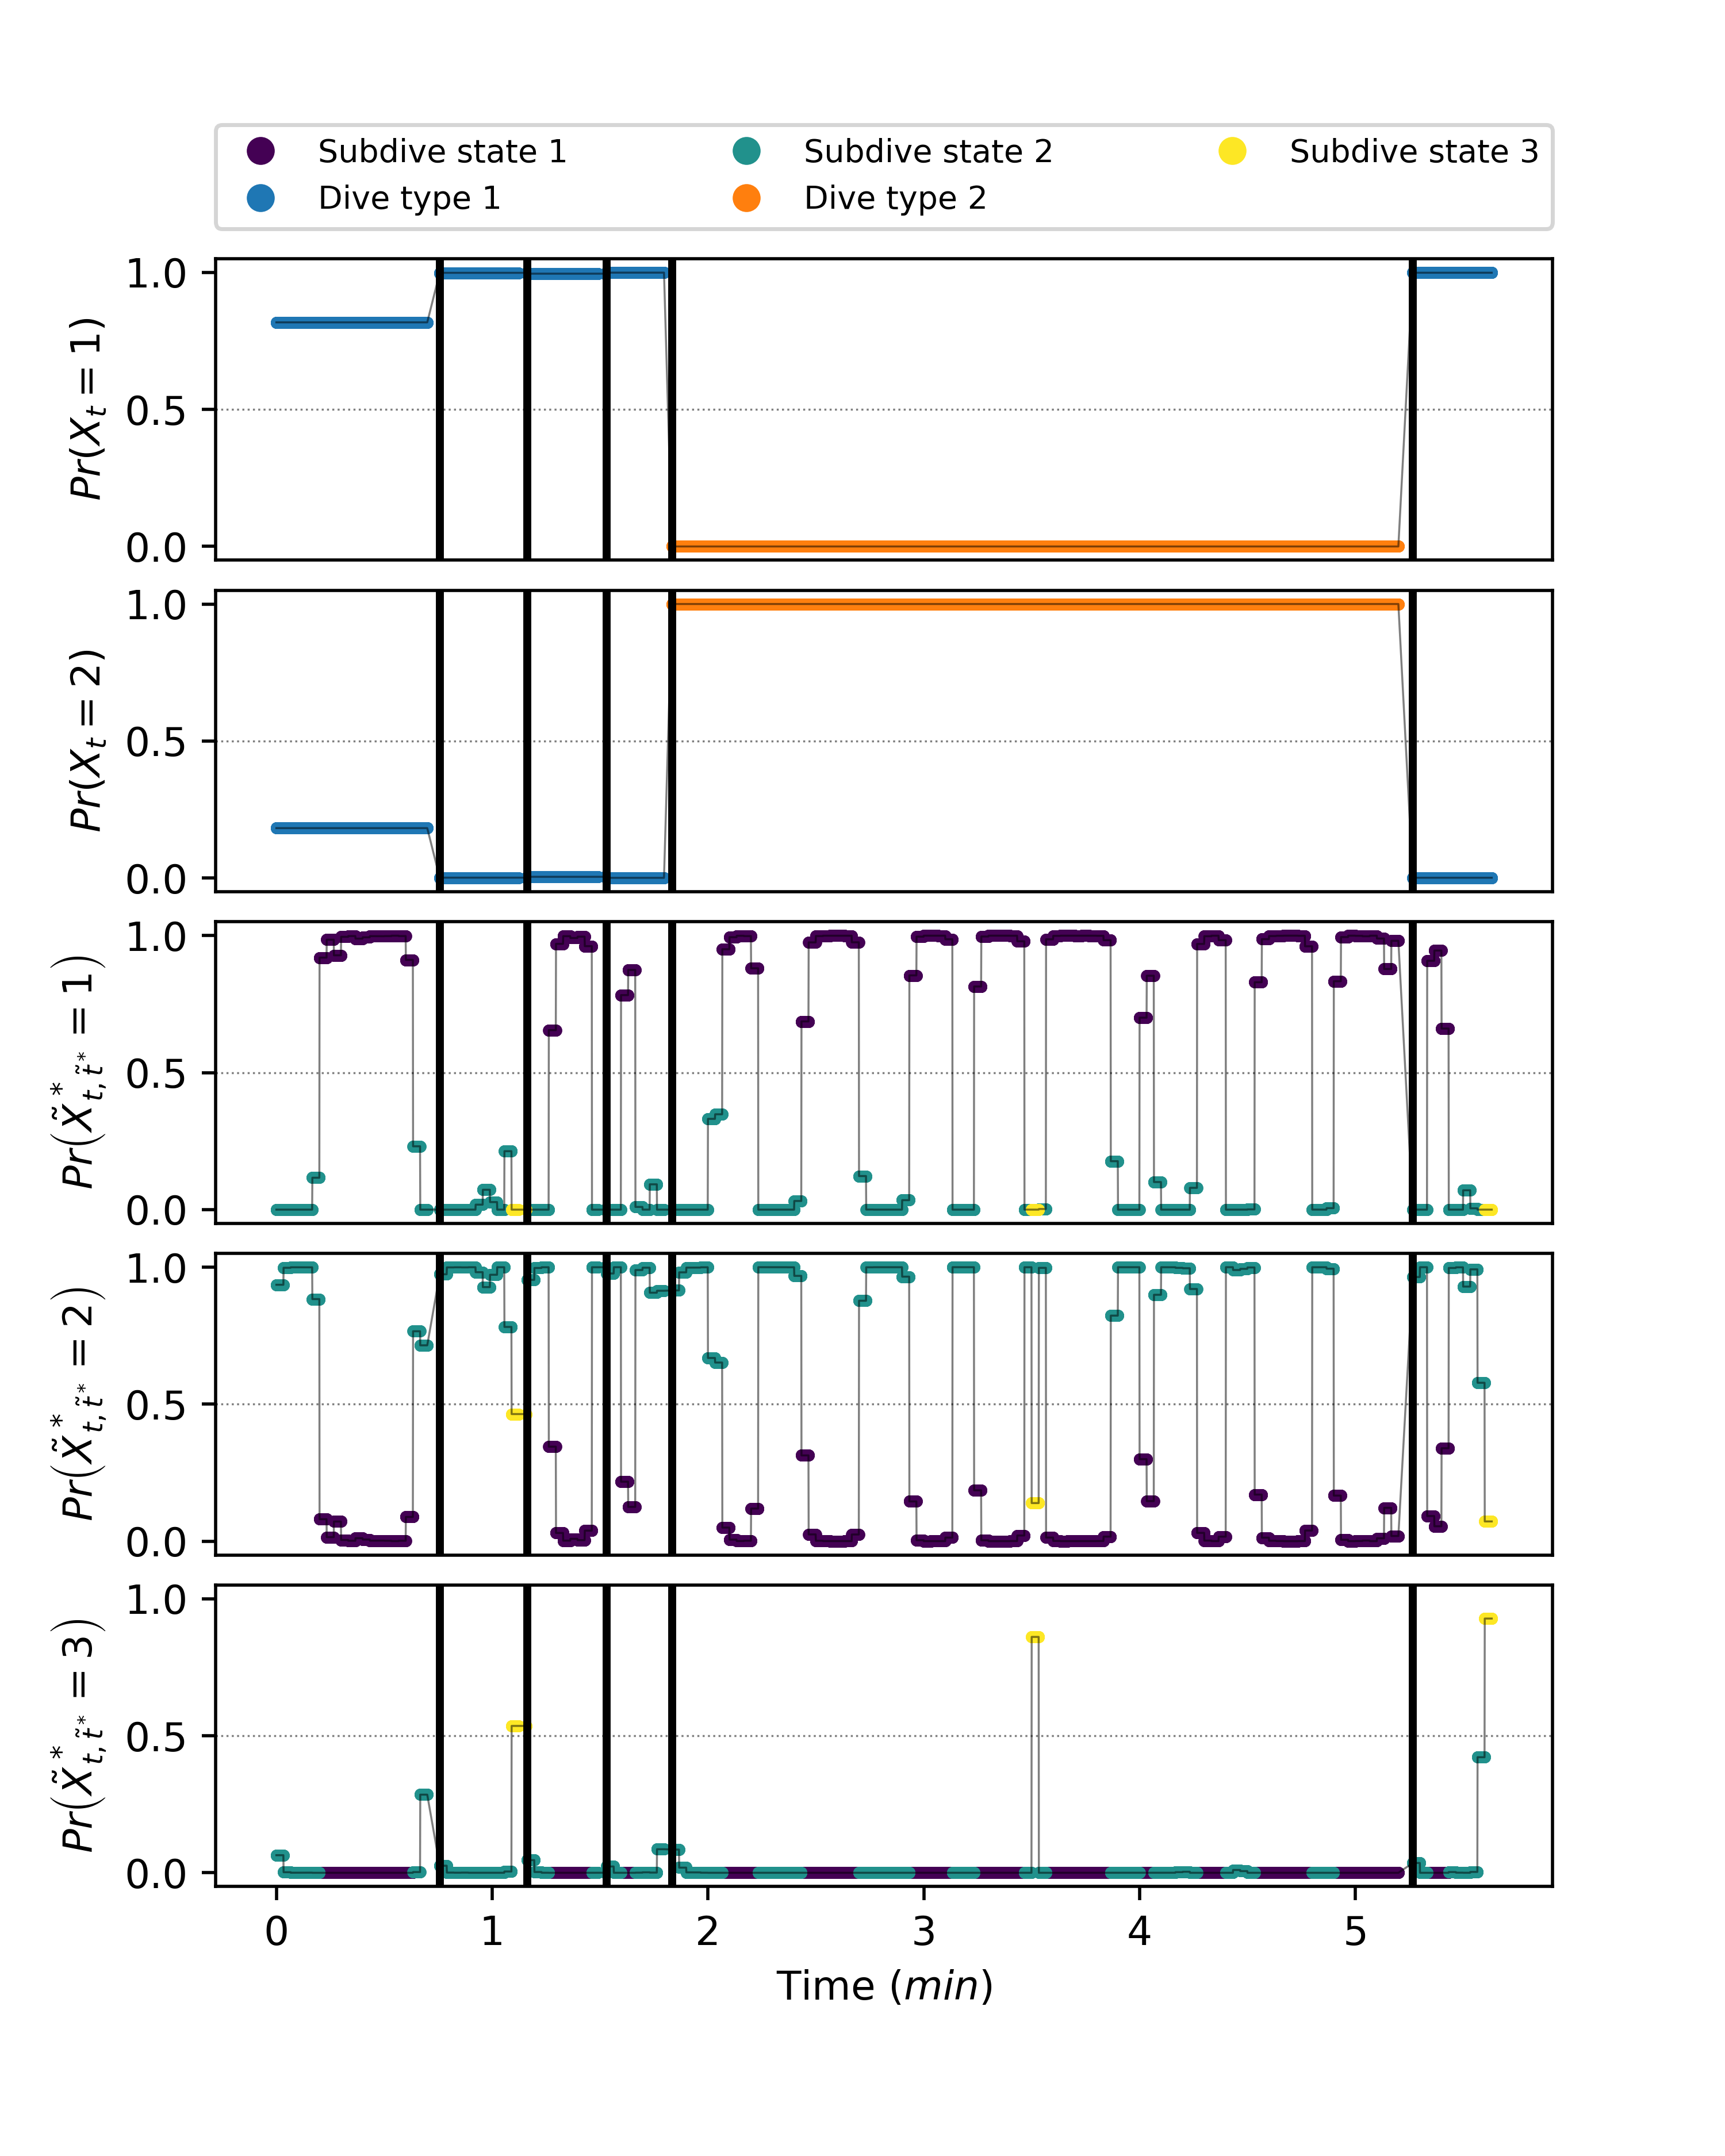
\includegraphics[width=6in]{../Plots/2019/20190902-182840-CATs_OB_1_0_267_CarHHMM2_decoded_states.png}
        \end{center}
        
        \noindent Figure \arabic{fignum}: The probability that each dive is a particular type or that the whale is in a particular subdive state, given the fitted model. Each panel is partitioned into dives by vertical black lines. The curve colours in the first and third panels correspond to the estimated dive types while the curve colours of the second and fourth panels correspond the estimated subdive states. Both the dive types and subdive states are estimated by fitting the CarHHMM-DFT to the data and performing the forward-backward algorithm.
        \addtocounter{fignum}{1}
        
        \subsection{HHMM-DFT}
        
        \begin{center}
        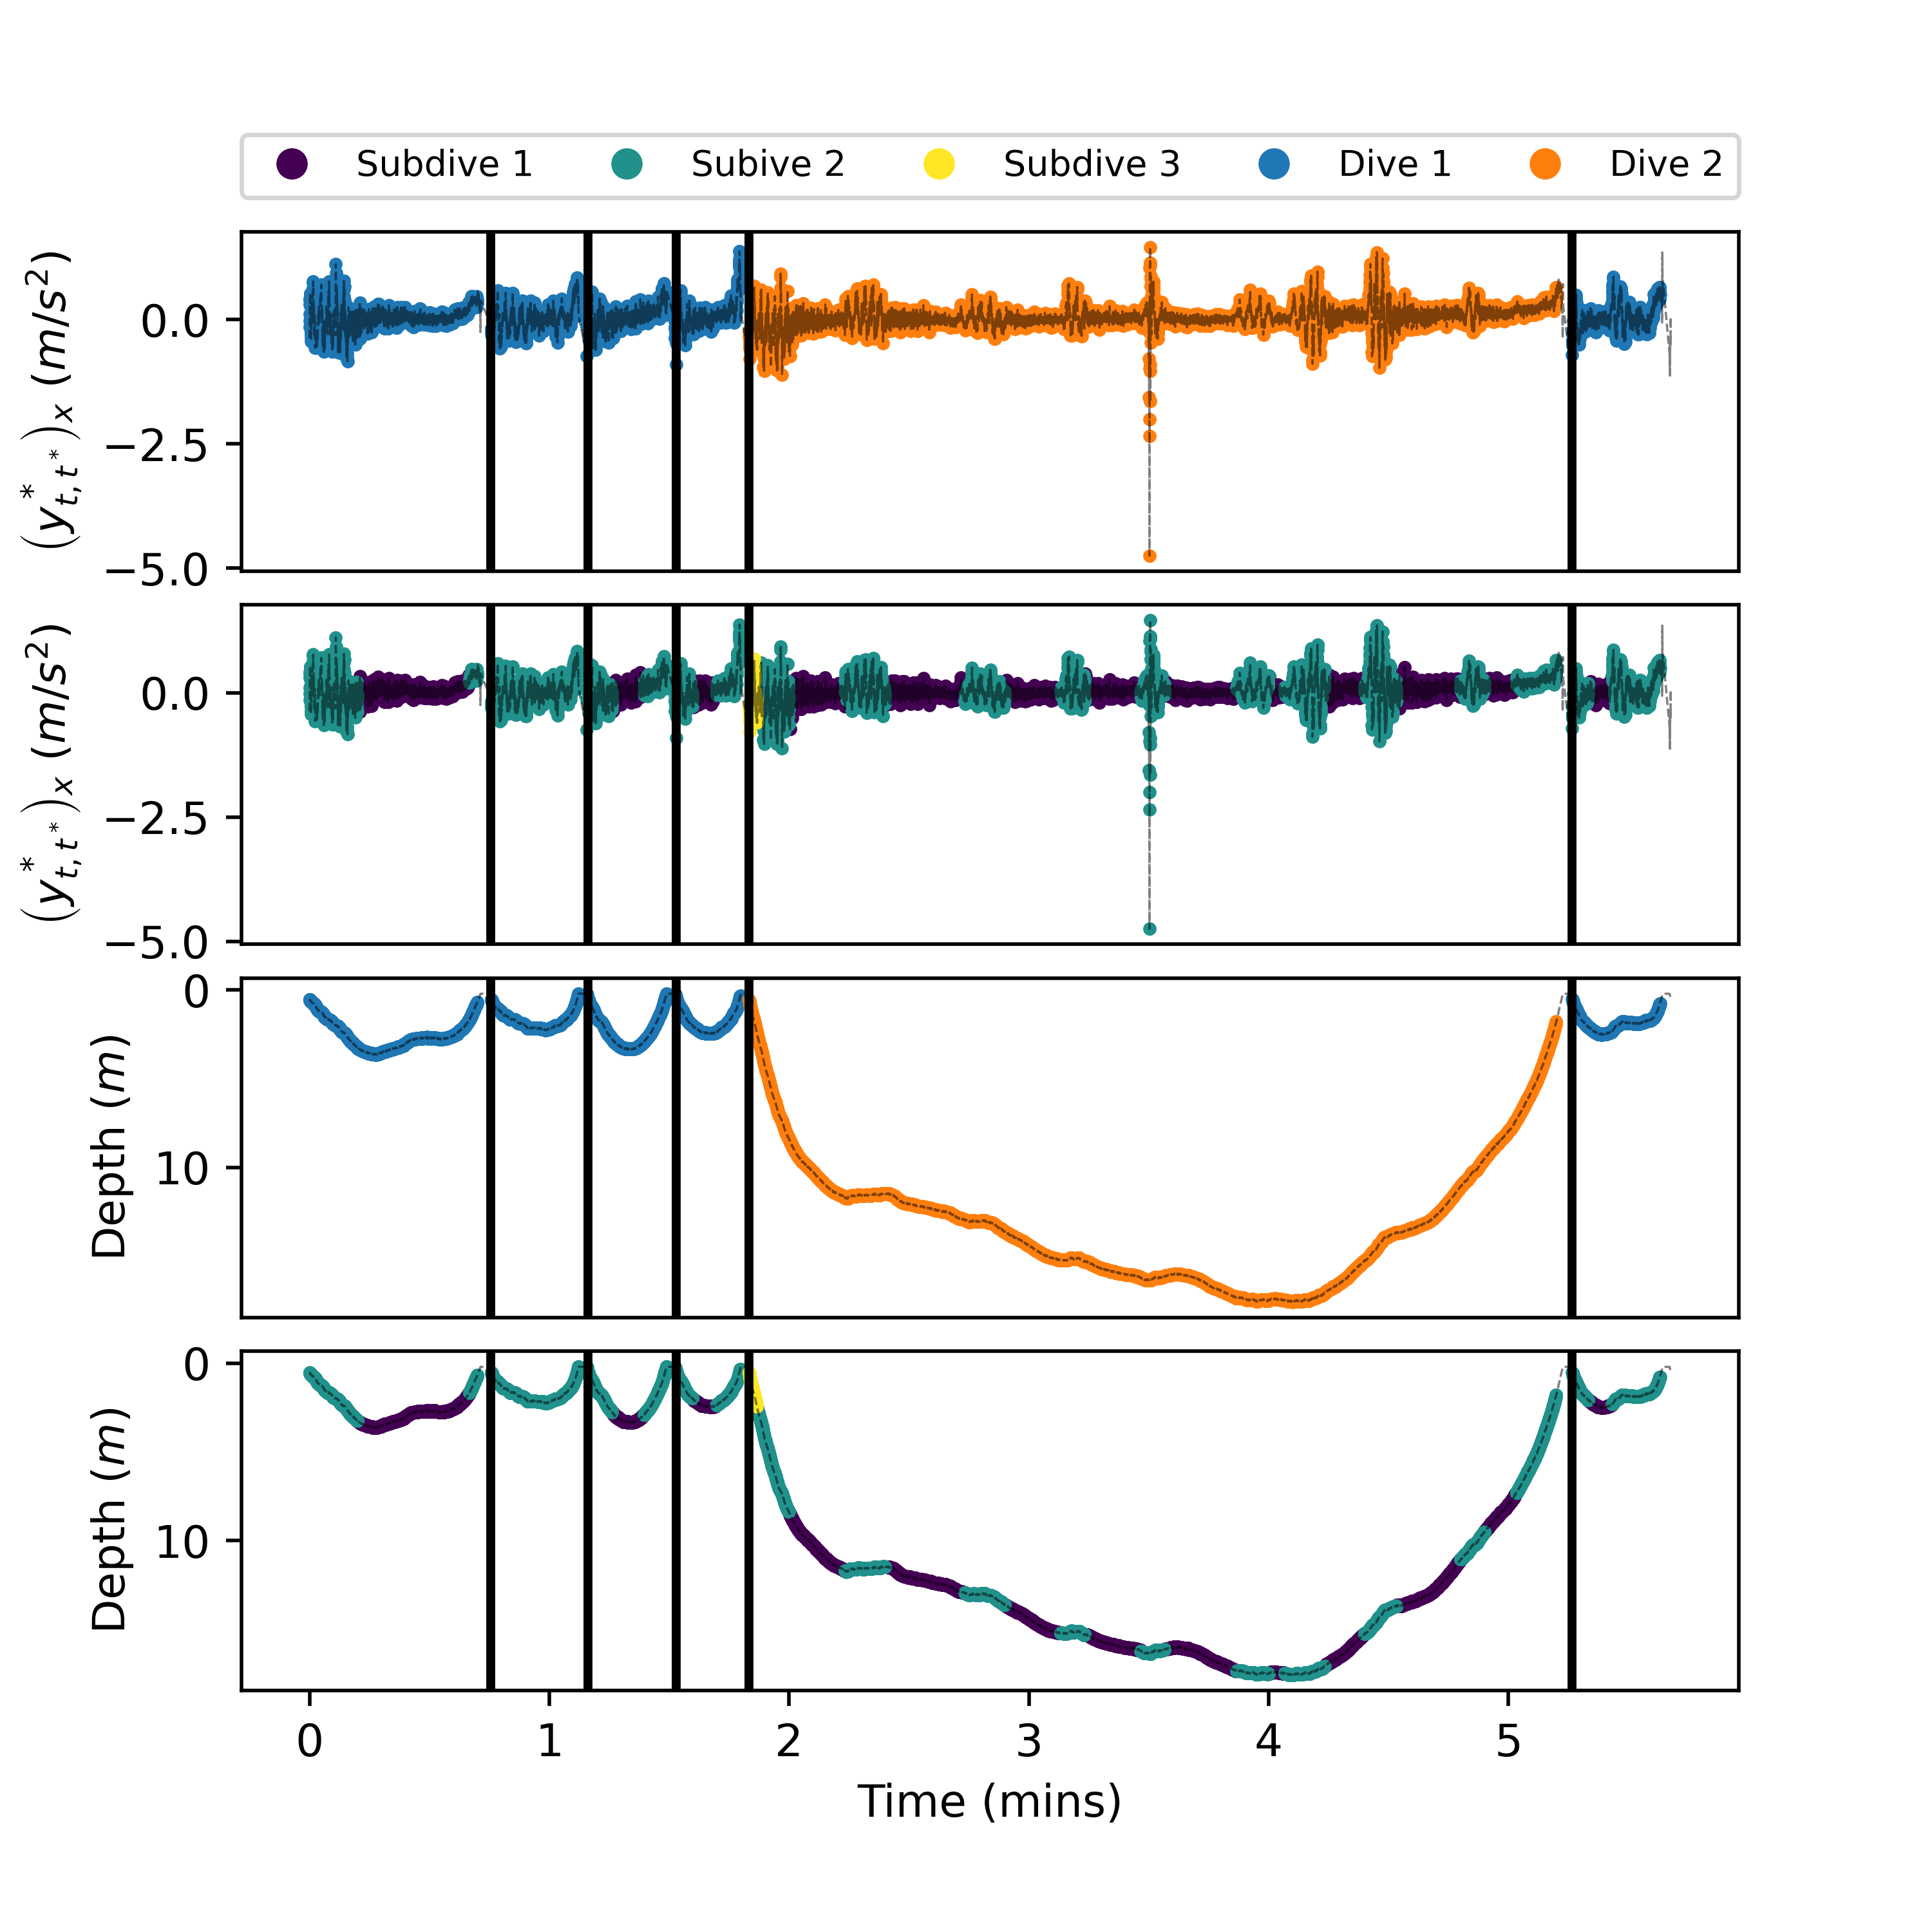
\includegraphics[width=6in]{../Plots/2019/20190902-182840-CATs_OB_1_0_267_HHMM_decoded_dives.png}
        \end{center}
        
        \noindent Figure \arabic{fignum}: The $x$--component of acceleration $(y^*_{t,t^*})_x$ (top two panels) and dive depth (bottom two panels) of a northern resident killer whale for a sequence of six selected dives. Each panel is partitioned into dives by vertical black lines. The curve colours in the first and third panels correspond to the estimated dive types while the curve colours of the second and fourth panels correspond the estimated subdive states. Both the dive types and subdive states are estimated by fitting the HHMM-DFT to the data and performing the forward-backward algorithm to determine the hidden state with the highest probability.
        \addtocounter{fignum}{1}
        
        \begin{center}
        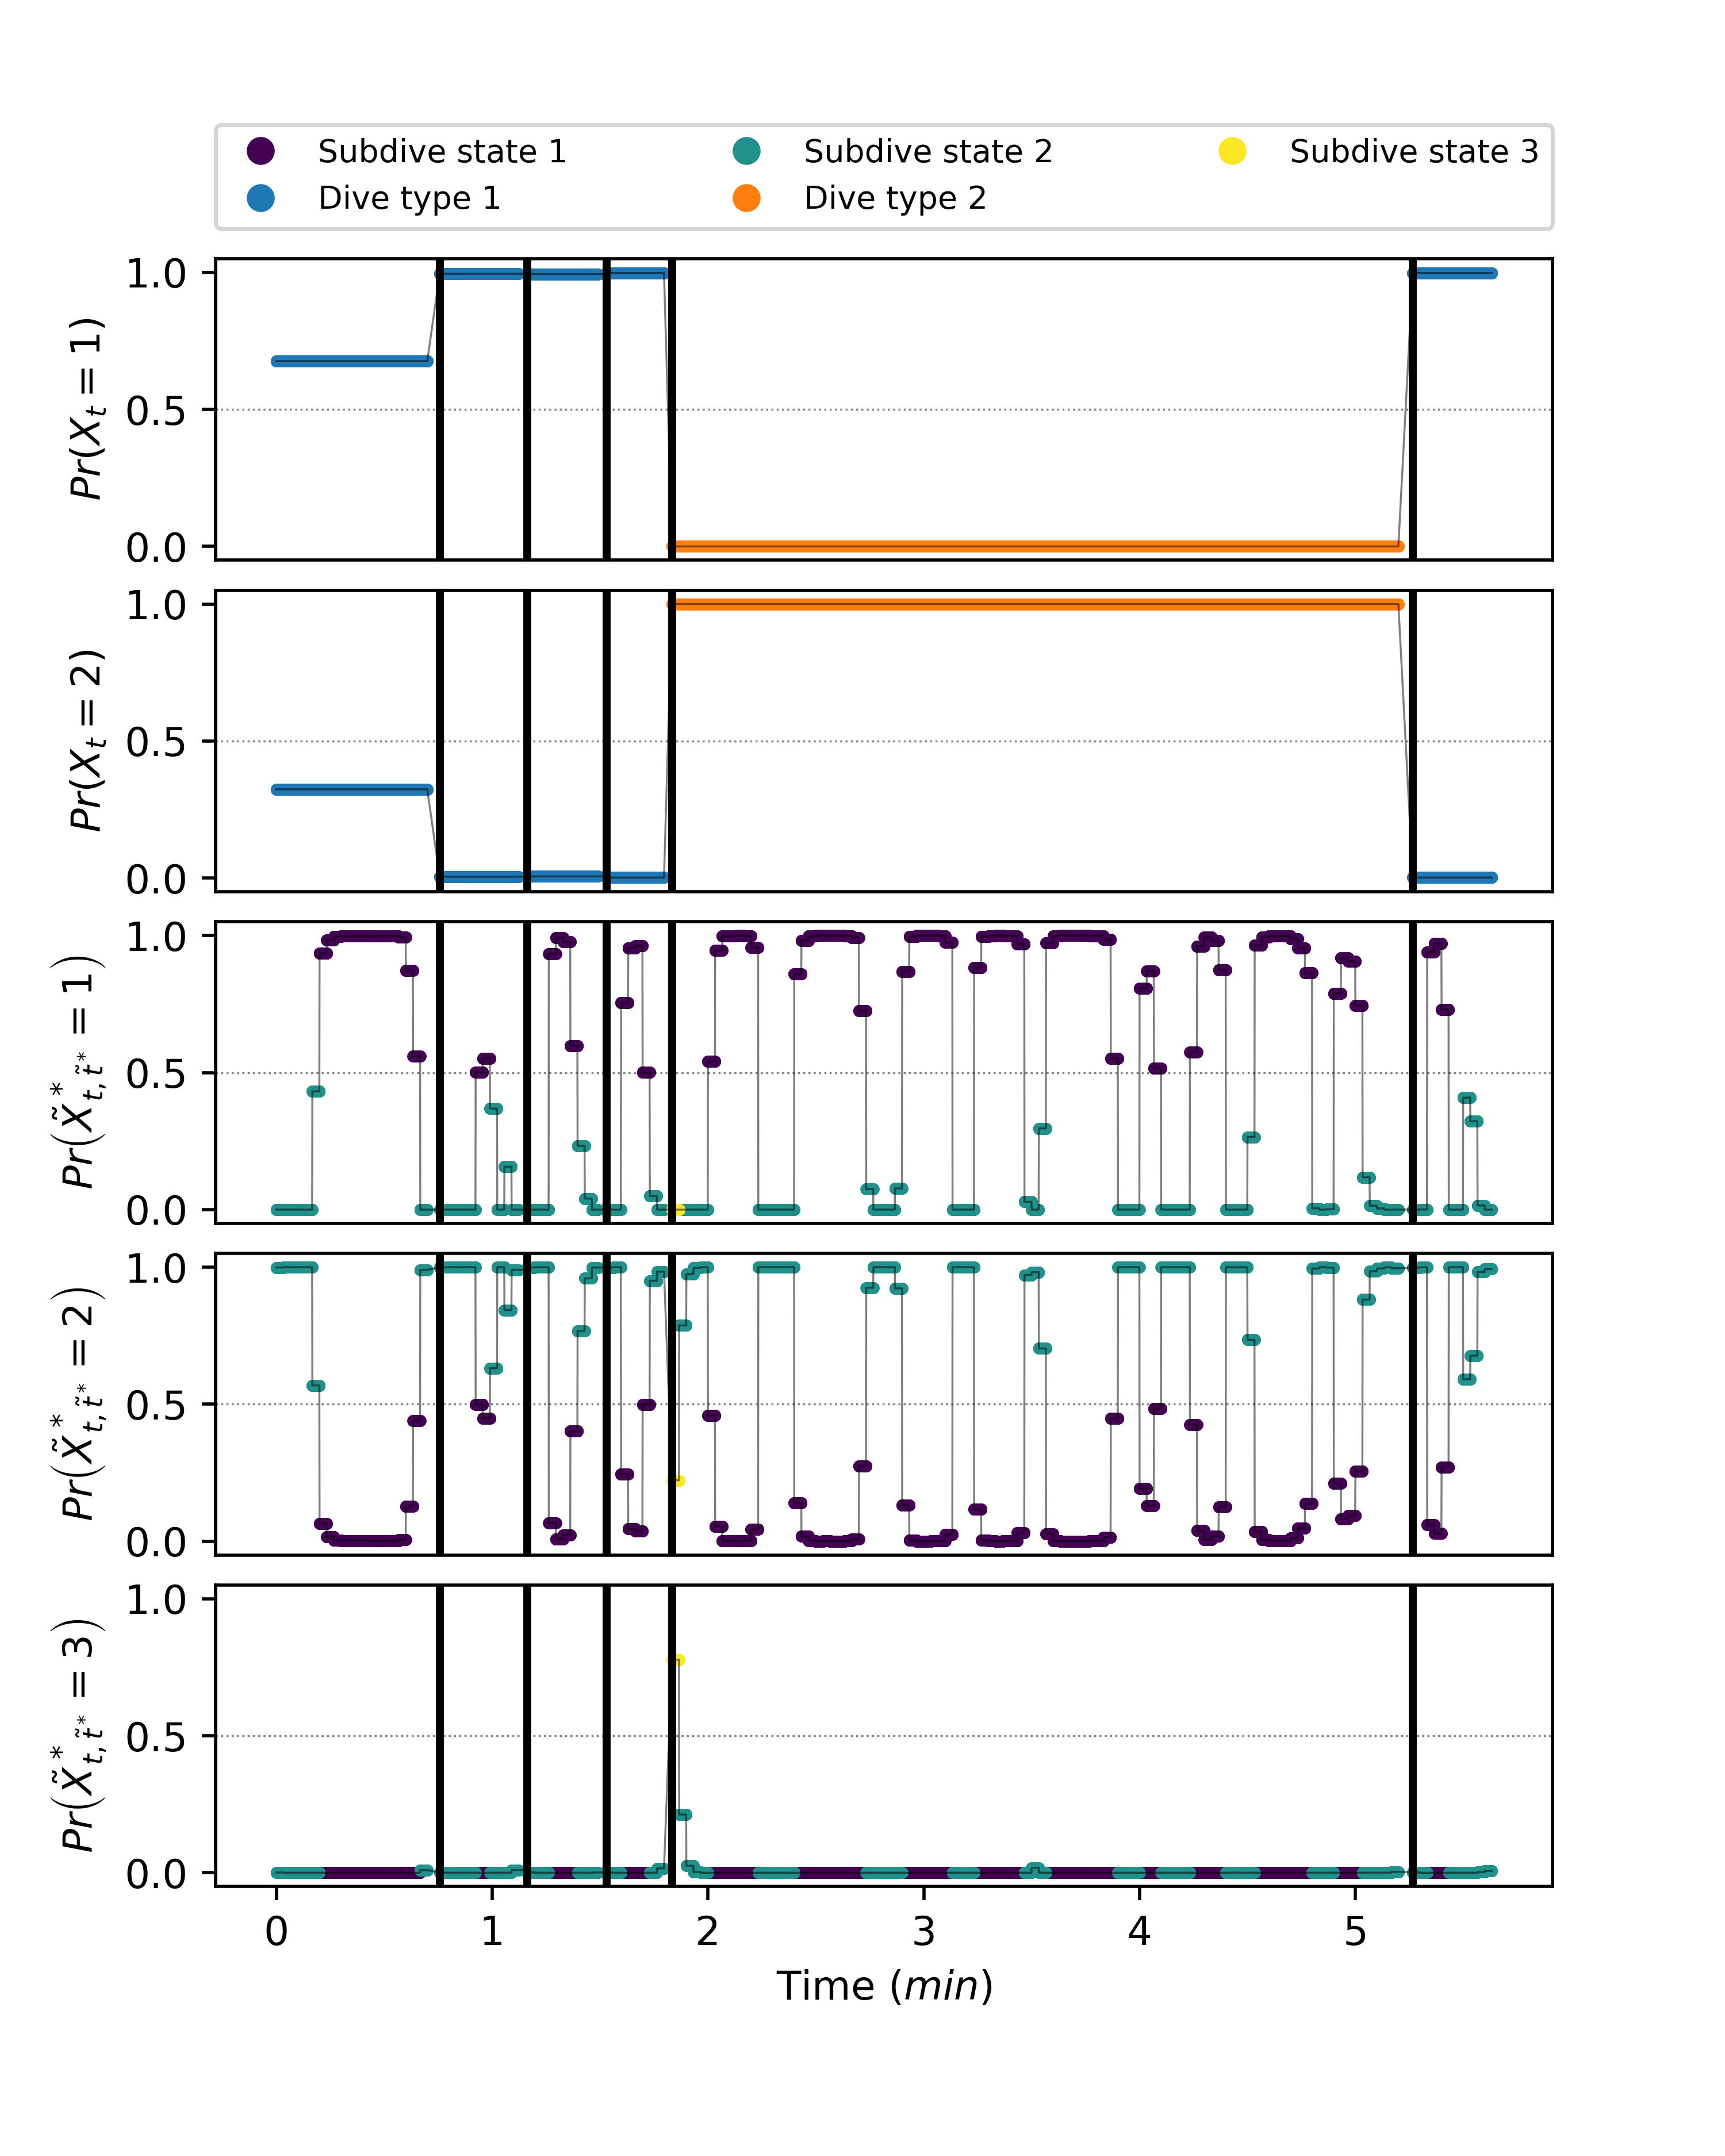
\includegraphics[width=6in]{../Plots/2019/20190902-182840-CATs_OB_1_0_267_HHMM_decoded_states.png}
        \end{center}
        
        \noindent Figure \arabic{fignum}: The probability that each dive is a particular type or that the whale is in a particular subdive state, given the fitted model. Each panel is partitioned into dives by vertical black lines. The curve colours in the first and third panels correspond to the estimated dive types while the curve colours of the second and fourth panels correspond the estimated subdive states. Both the dive types and subdive states are estimated by fitting the HHMM-DFT to the data and performing the forward-backward algorithm.
        \addtocounter{fignum}{1}
        
        \subsection{CarHHMM}
        
        \begin{center}
        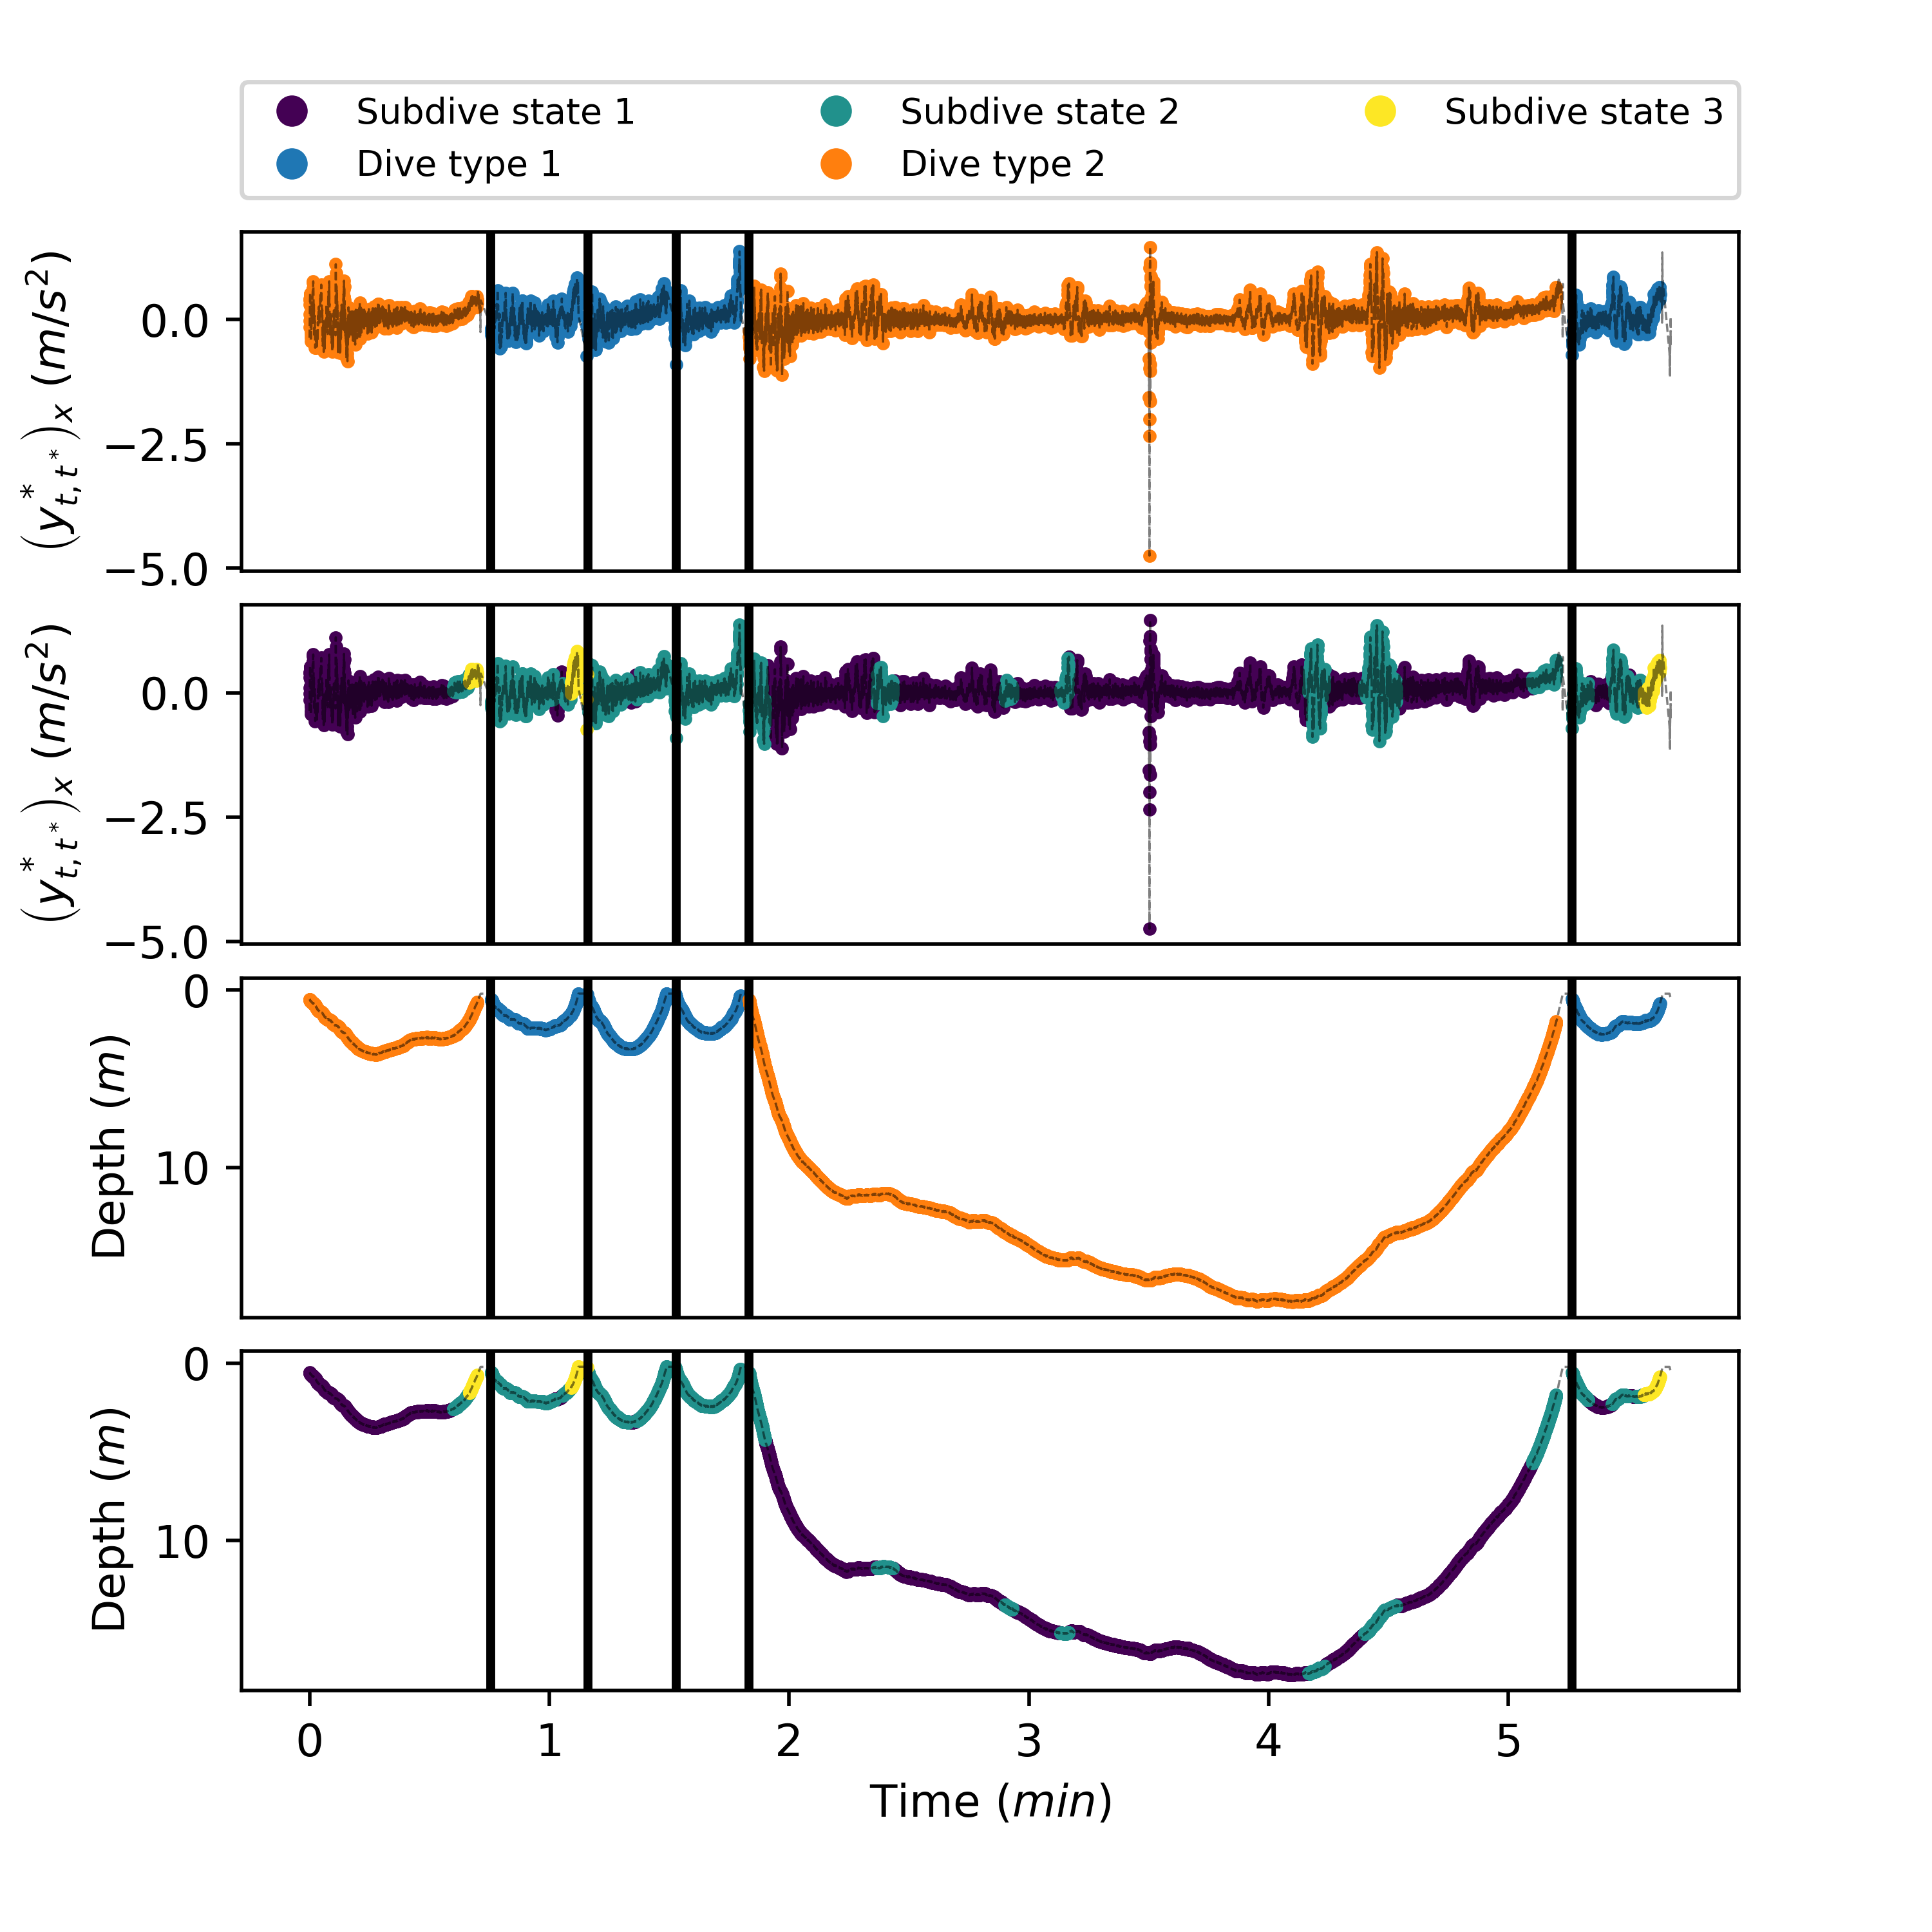
\includegraphics[width=6in]{../Plots/2019/20190902-182840-CATs_OB_1_0_267_CarHHMM1_decoded_dives.png}
        \end{center}
        
        \noindent Figure \arabic{fignum}: The $x$--component of acceleration $(y^*_{t,t^*})_x$ (top two panels) and dive depth (bottom two panels) of a northern resident killer whale for a sequence of six selected dives. Each panel is partitioned into dives by vertical black lines. The curve colours in the first and third panels correspond to the estimated dive types while the curve colours of the second and fourth panels correspond the estimated subdive states. Both the dive types and subdive states are estimated by fitting the CarHHMM to the data and performing the forward-backward algorithm to determine the hidden state with the highest probability.
        \addtocounter{fignum}{1}
        
        \begin{center}
        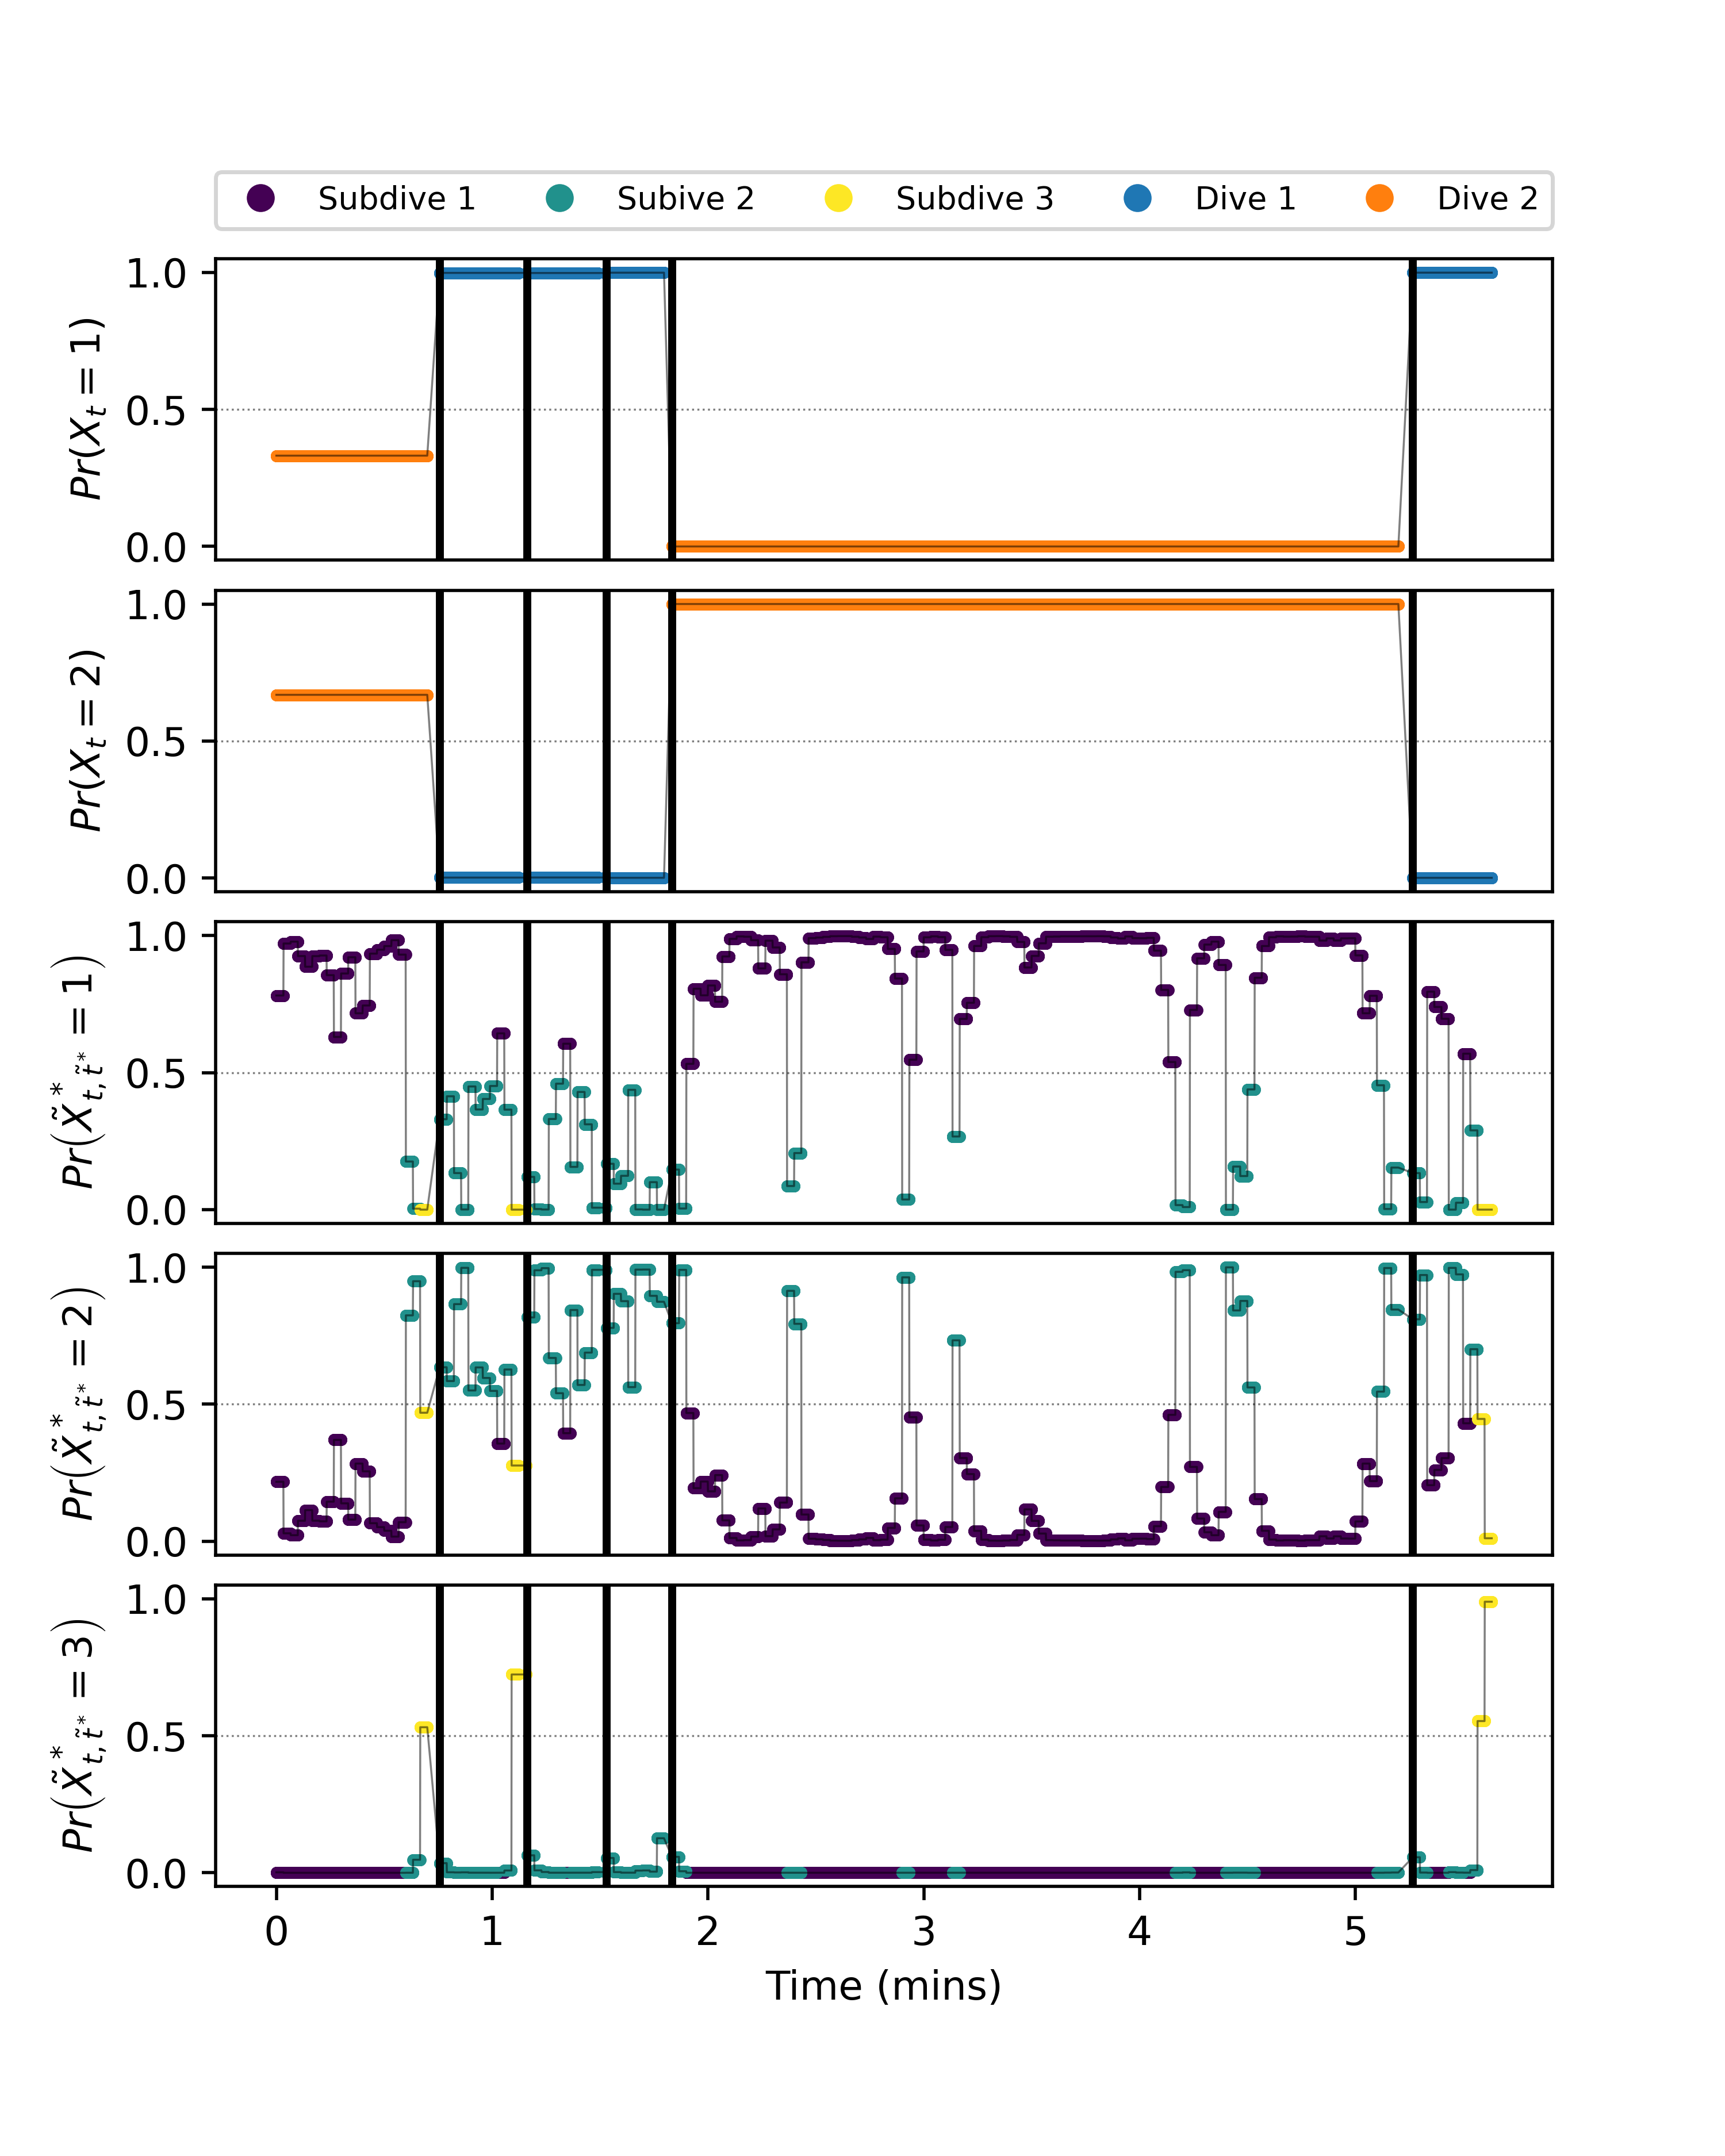
\includegraphics[width=6in]{../Plots/2019/20190902-182840-CATs_OB_1_0_267_CarHHMM1_decoded_states.png}
        \end{center}
        
        \noindent Figure \arabic{fignum}: The probability that each dive is a particular type or that the whale is in a particular subdive state, given the fitted model. Each panel is partitioned into dives by vertical black lines. The curve colours in the first and third panels correspond to the estimated dive types while the curve colours of the second and fourth panels correspond the estimated subdive states. Both the dive types and subdive states are estimated by fitting the CarHHMM to the data and performing the forward-backward algorithm.
        \addtocounter{fignum}{1}
        
        \subsection{CarHMM-DFT}
        
        \begin{center}
        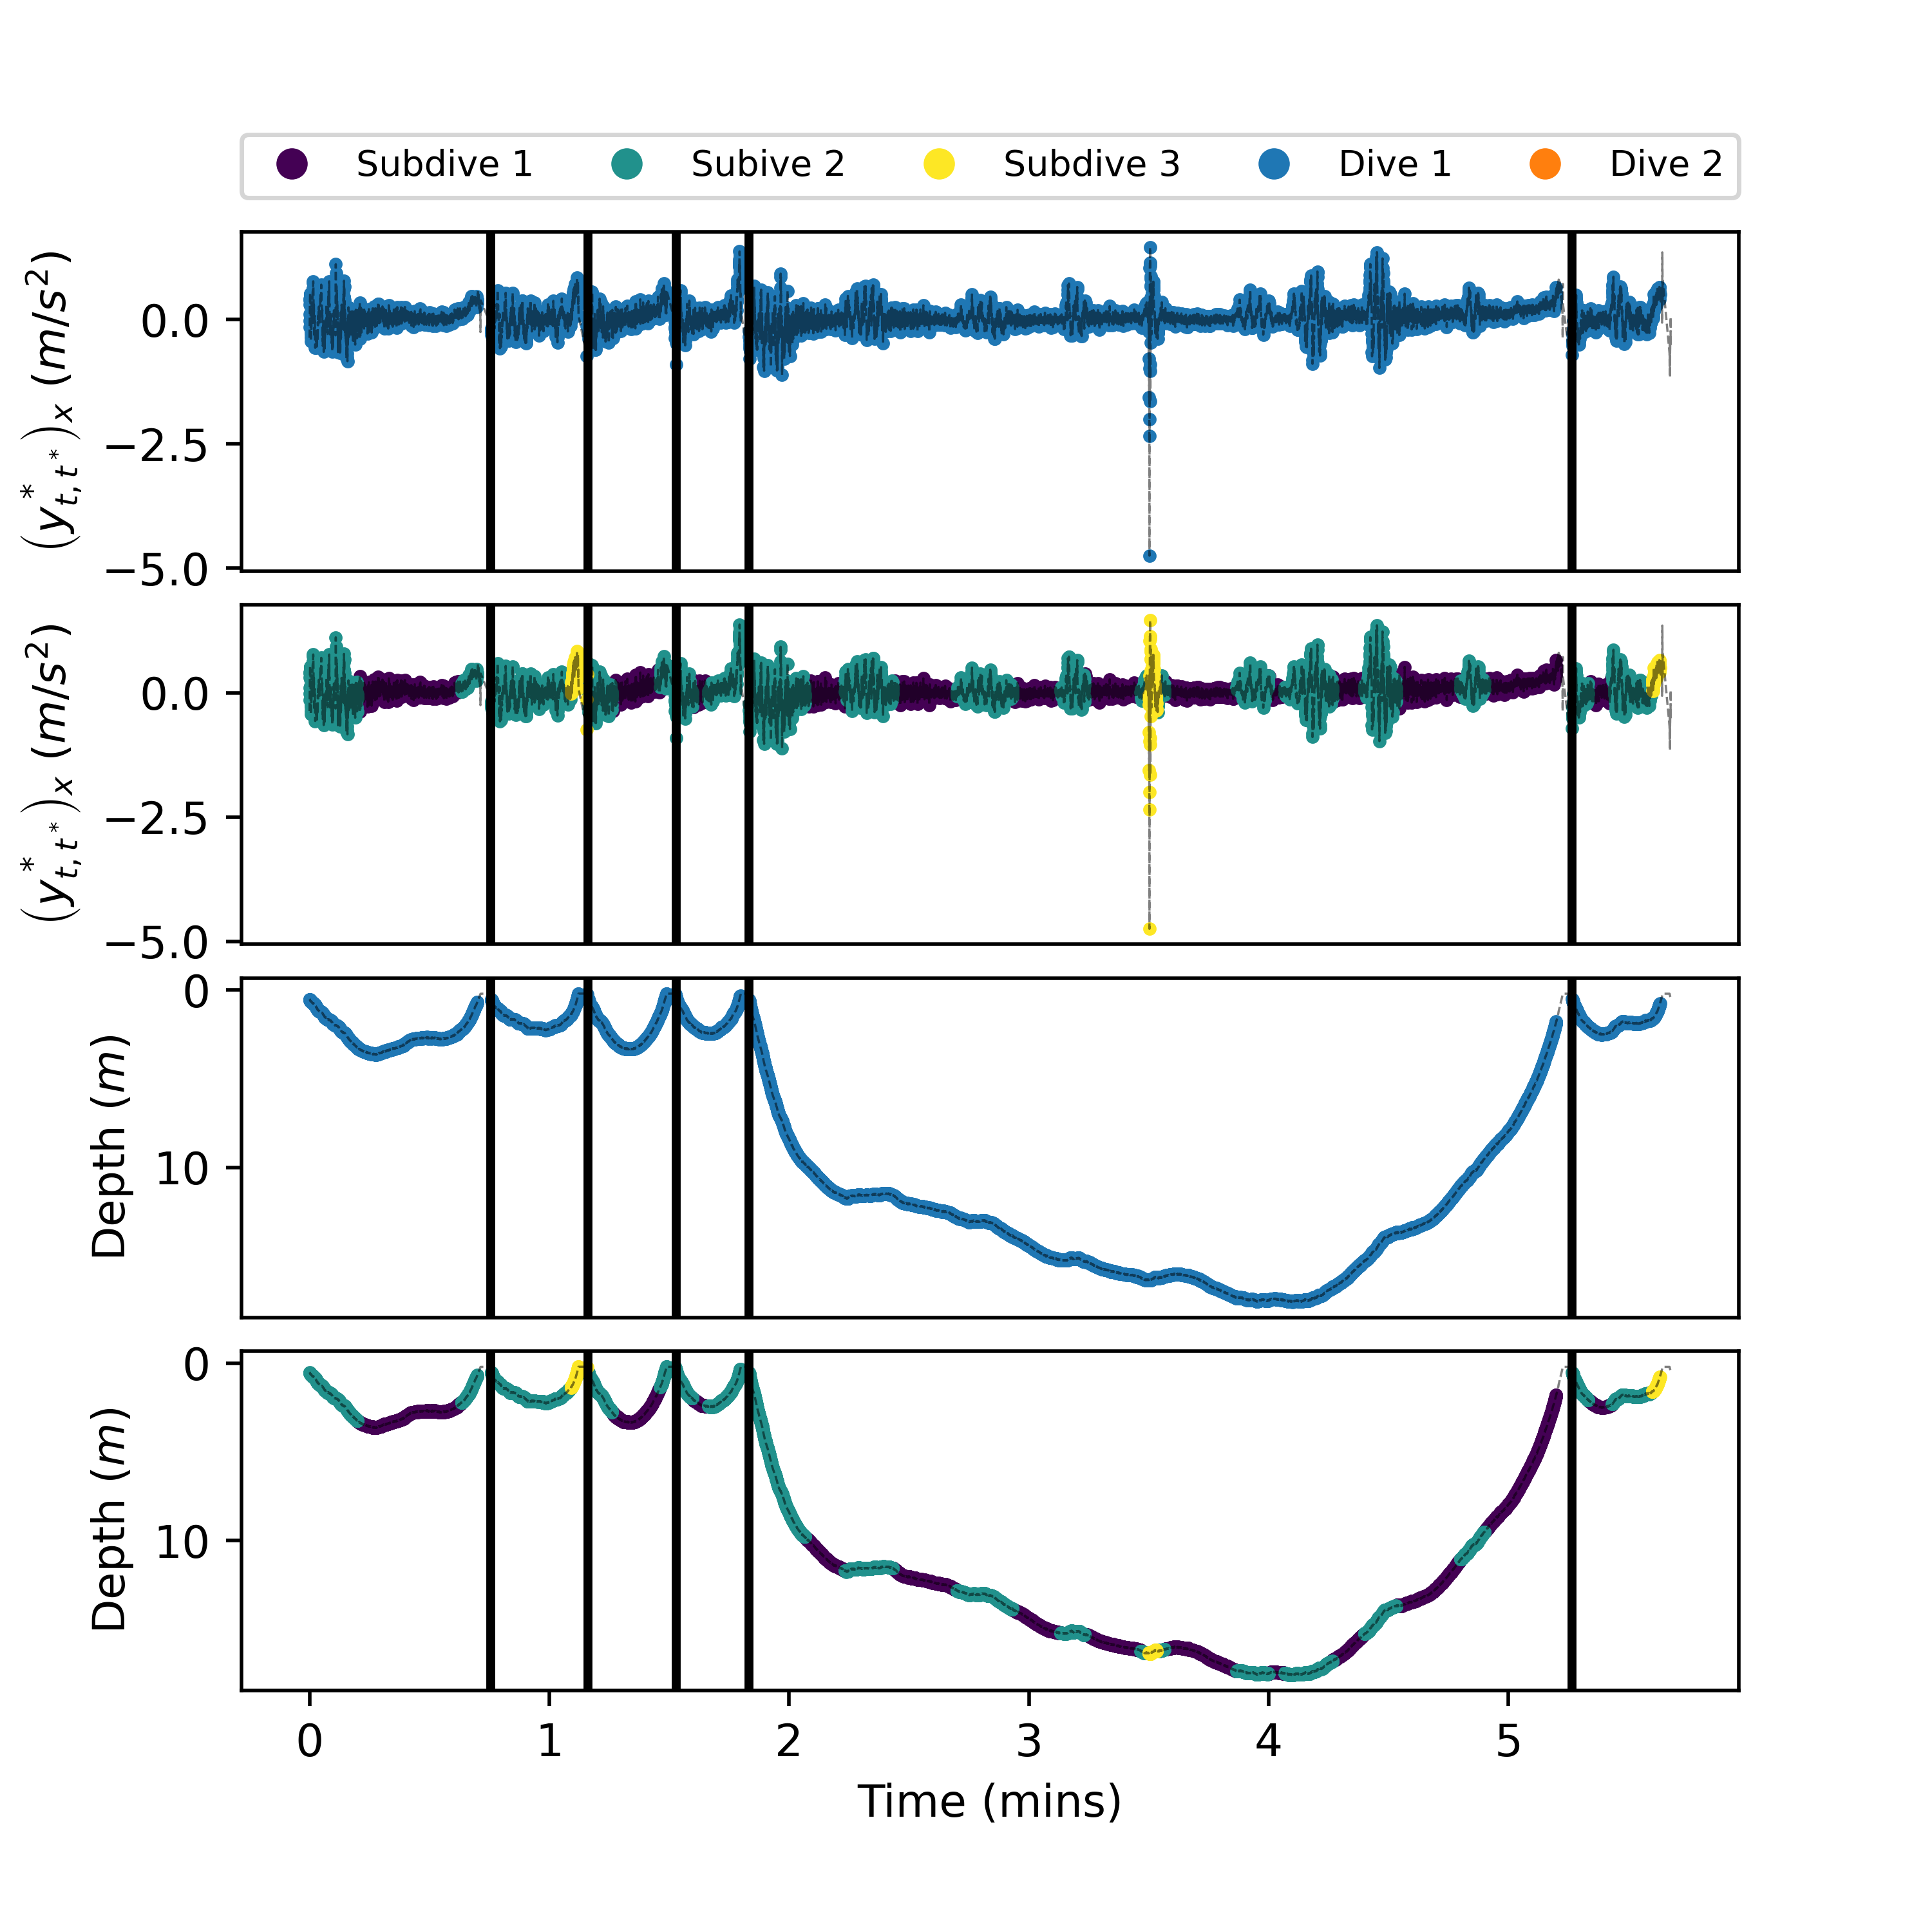
\includegraphics[width=6in]{../Plots/2019/20190902-182840-CATs_OB_1_0_267_CarHMM_decoded_dives.png}
        \end{center}
        
        \noindent Figure \arabic{fignum}: The $x$--component of acceleration $(y^*_{t,t^*})_x$ (top two panels) and dive depth (bottom two panels) of a northern resident killer whale for a sequence of six selected dives. Each panel is partitioned into dives by vertical black lines. The curve colours in the first and third panels correspond to the estimated dive types while the curve colours of the second and fourth panels correspond the estimated subdive states. Both the dive types and subdive states are estimated by fitting the CarHMM-DFT to the data and performing the forward-backward algorithm to determine the hidden state with the highest probability.
        \addtocounter{fignum}{1}
        
        \begin{center}
        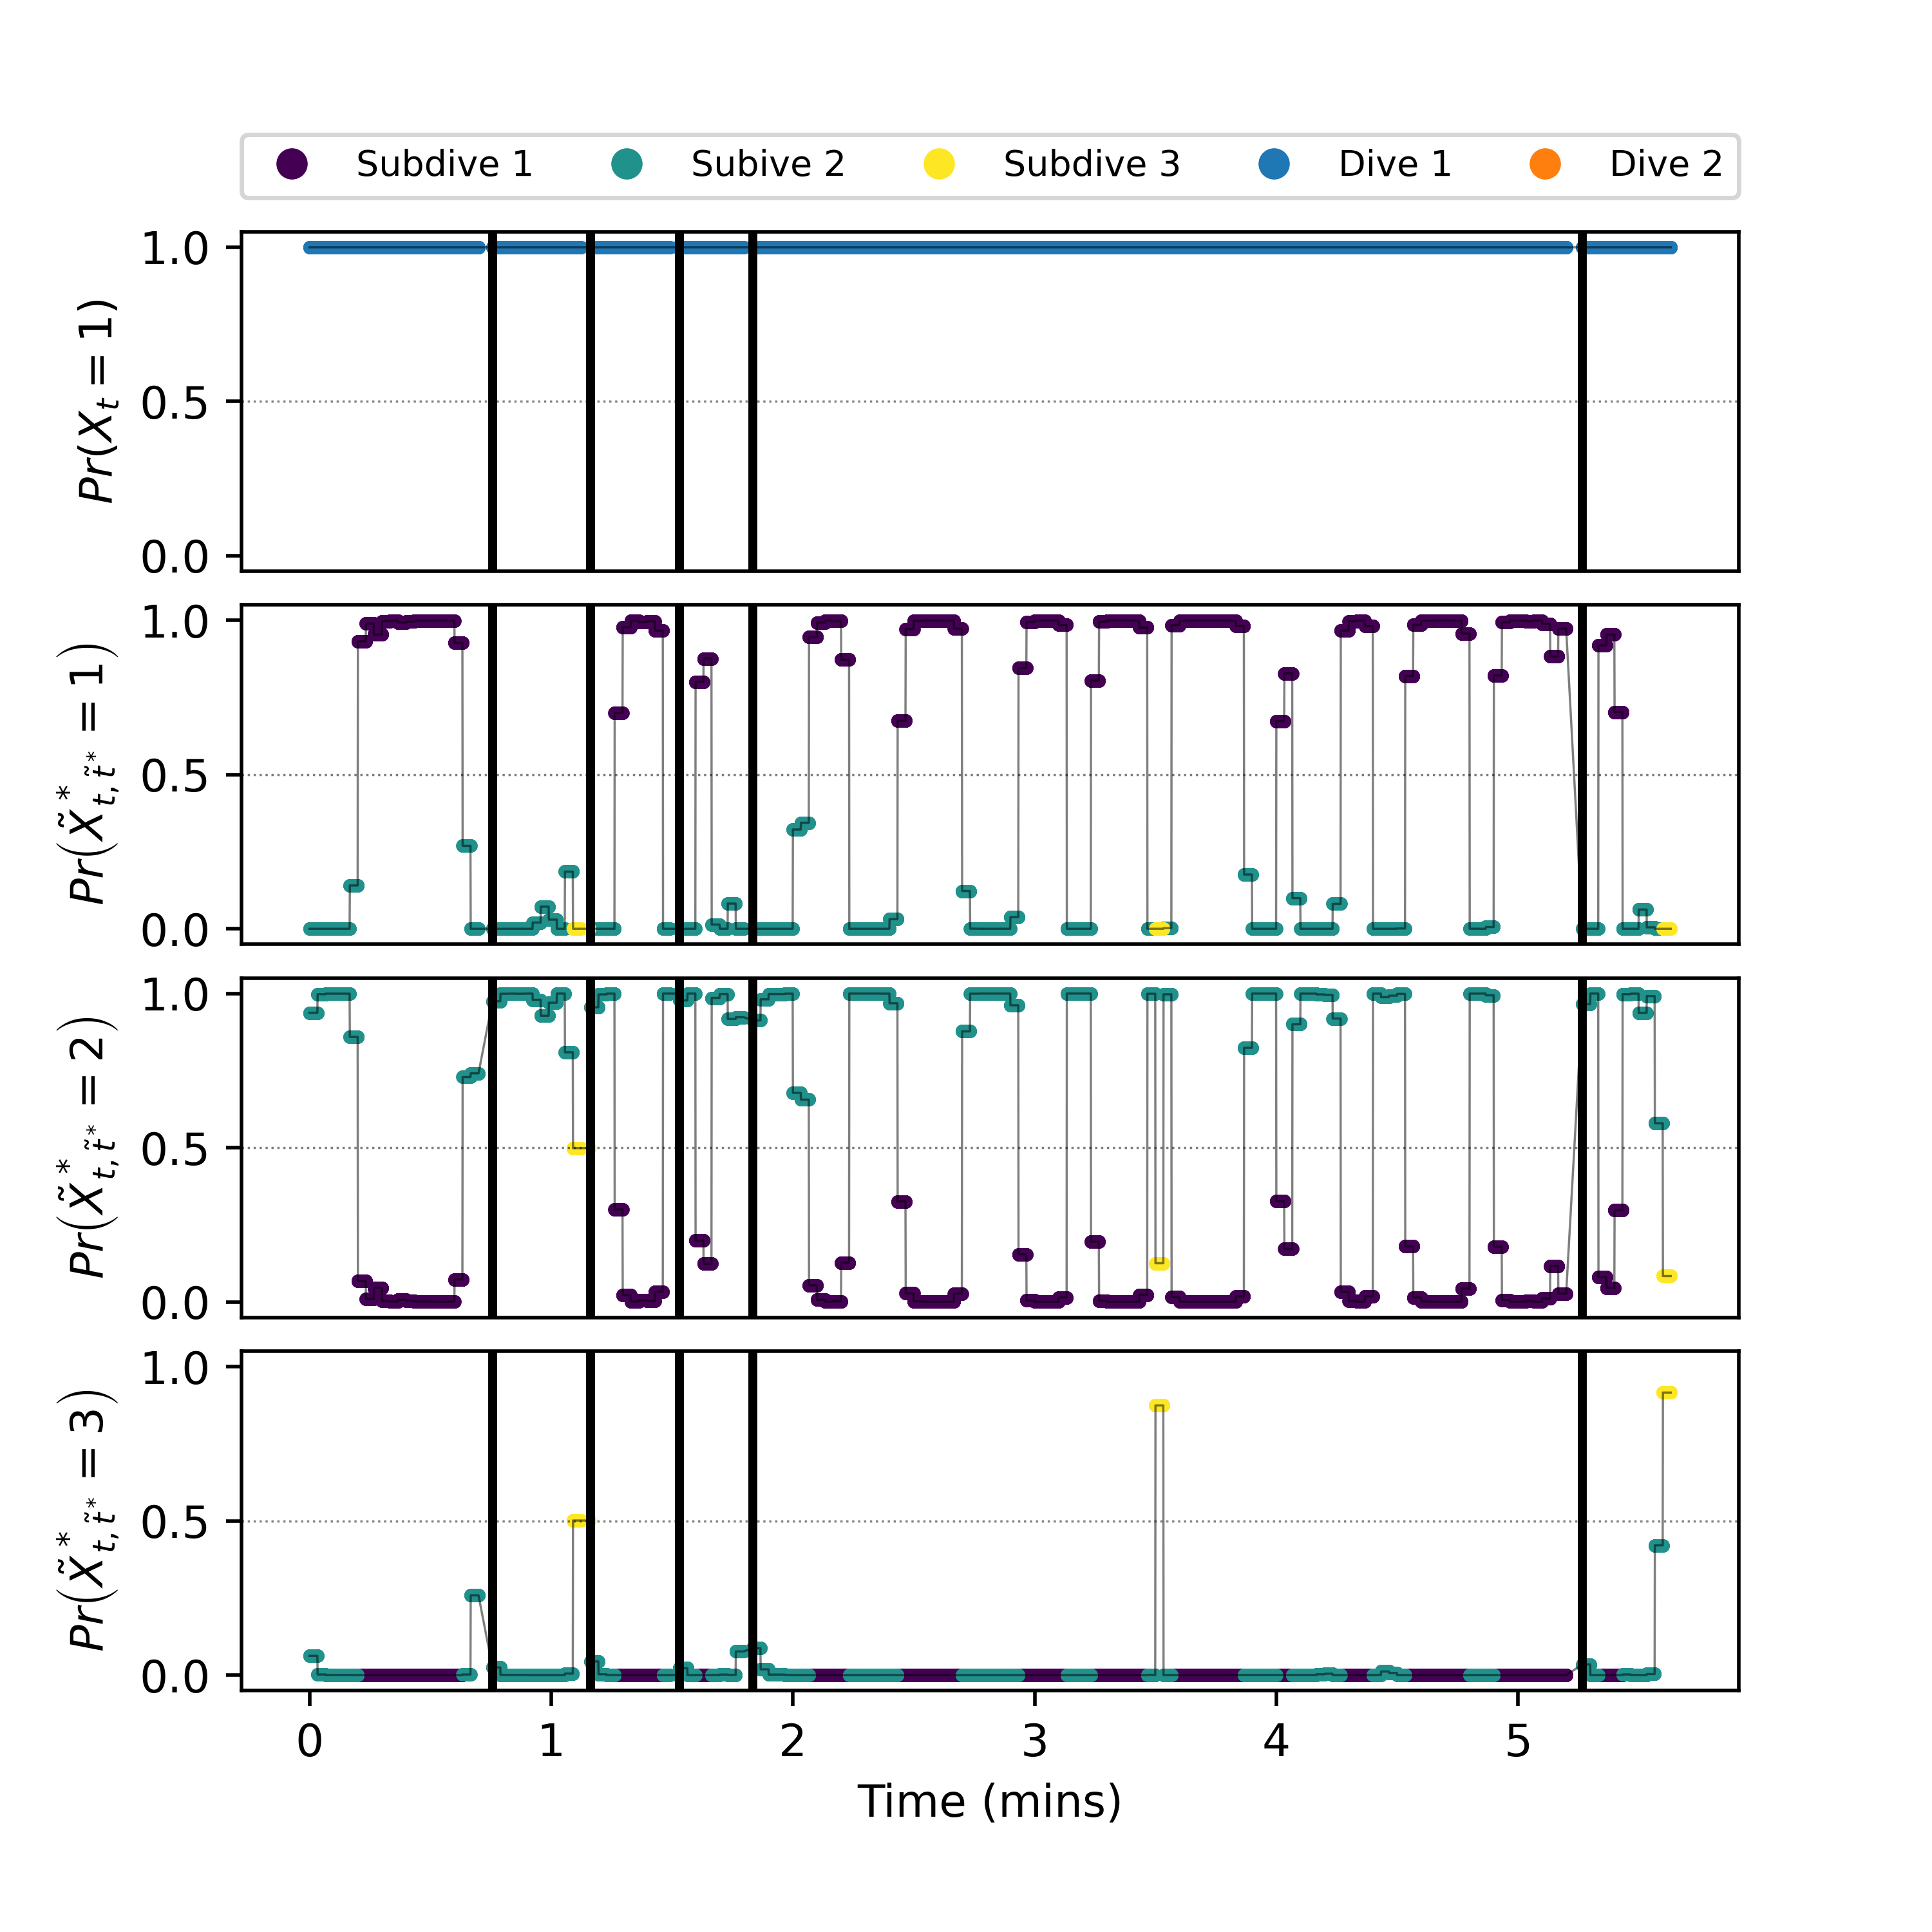
\includegraphics[width=6in]{../Plots/2019/20190902-182840-CATs_OB_1_0_267_CarHMM_decoded_states.png}
        \end{center}
        
        \noindent Figure \arabic{fignum}: The probability that each dive is a particular type or that the whale is in a particular subdive state, given the fitted model. Each panel is partitioned into dives by vertical black lines. The curve colours in the first and third panels correspond to the estimated dive types while the curve colours of the second and fourth panels correspond the estimated subdive states. Both the dive types and subdive states are estimated by fitting the CarHMM-DFT to the data and performing the forward-backward algorithm.
        \addtocounter{fignum}{1}
        
    \newpage
    \section{Model checking - dive duration ($Y_t$)}
    
        \subsection{CarHHMM-DFT}
        
        \begin{center}
        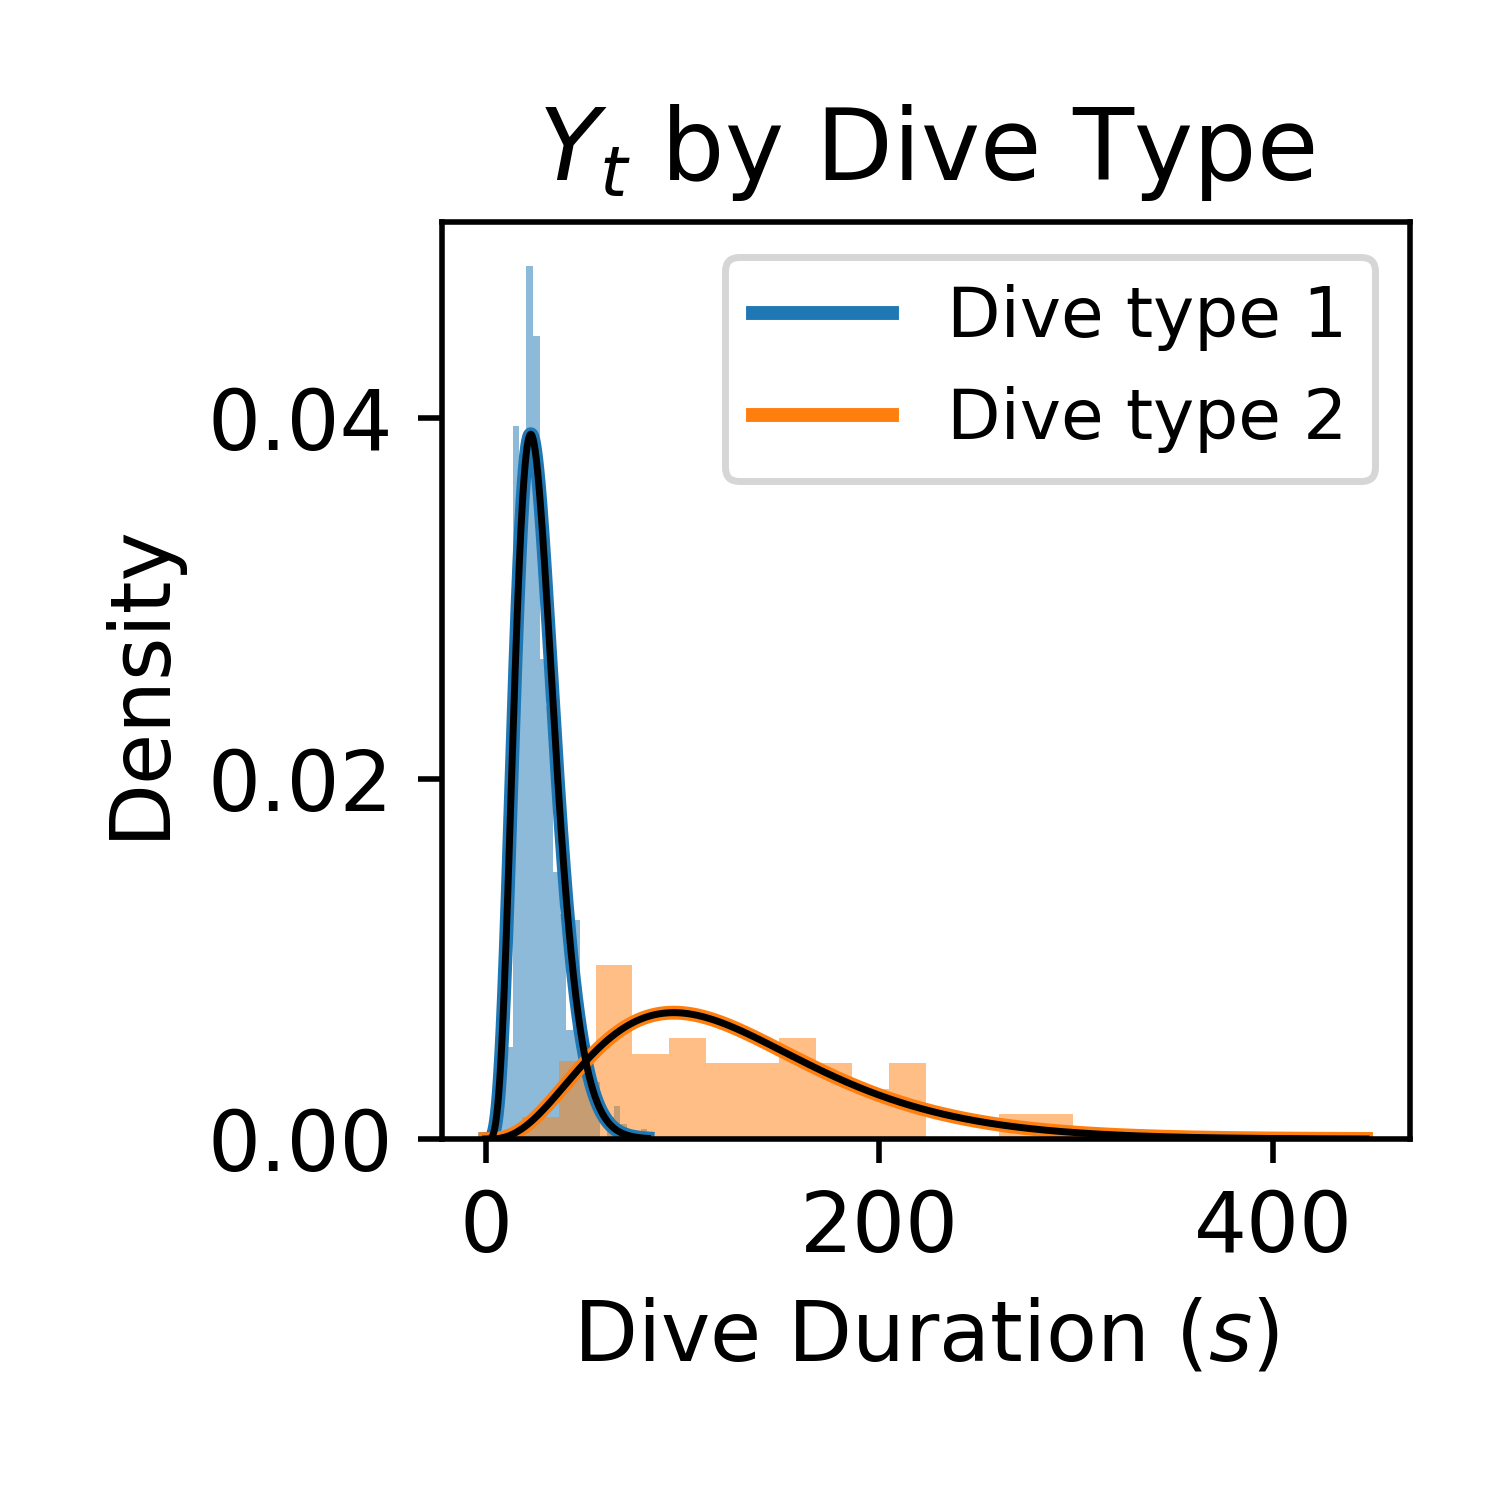
\includegraphics[width=2.25in]{../Plots/2019/20190902-182840-CATs_OB_1_0_267_CarHHMM2_empirical_hist_dive_duration.png}
        \includegraphics[width=2.25in]{../Plots/2019/20190902-182840-CATs_OB_1_0_267_CarHHMM2_pseudresids_Dive_Duration.png}
        \end{center}
        
        \noindent Figure \arabic{fignum}: Empirical histogram (left) and psuedoresiduals (right) of dive duration ($Y_{t}$) plotted over the estimated emission distributions and a standard normal density, respectively. Both plots are generated using the fitted CarHHMM-DFT and the killer whale case study data.
        \addtocounter{fignum}{1}
        
        \subsection{HHMM-DFT}
        
        \begin{center}
        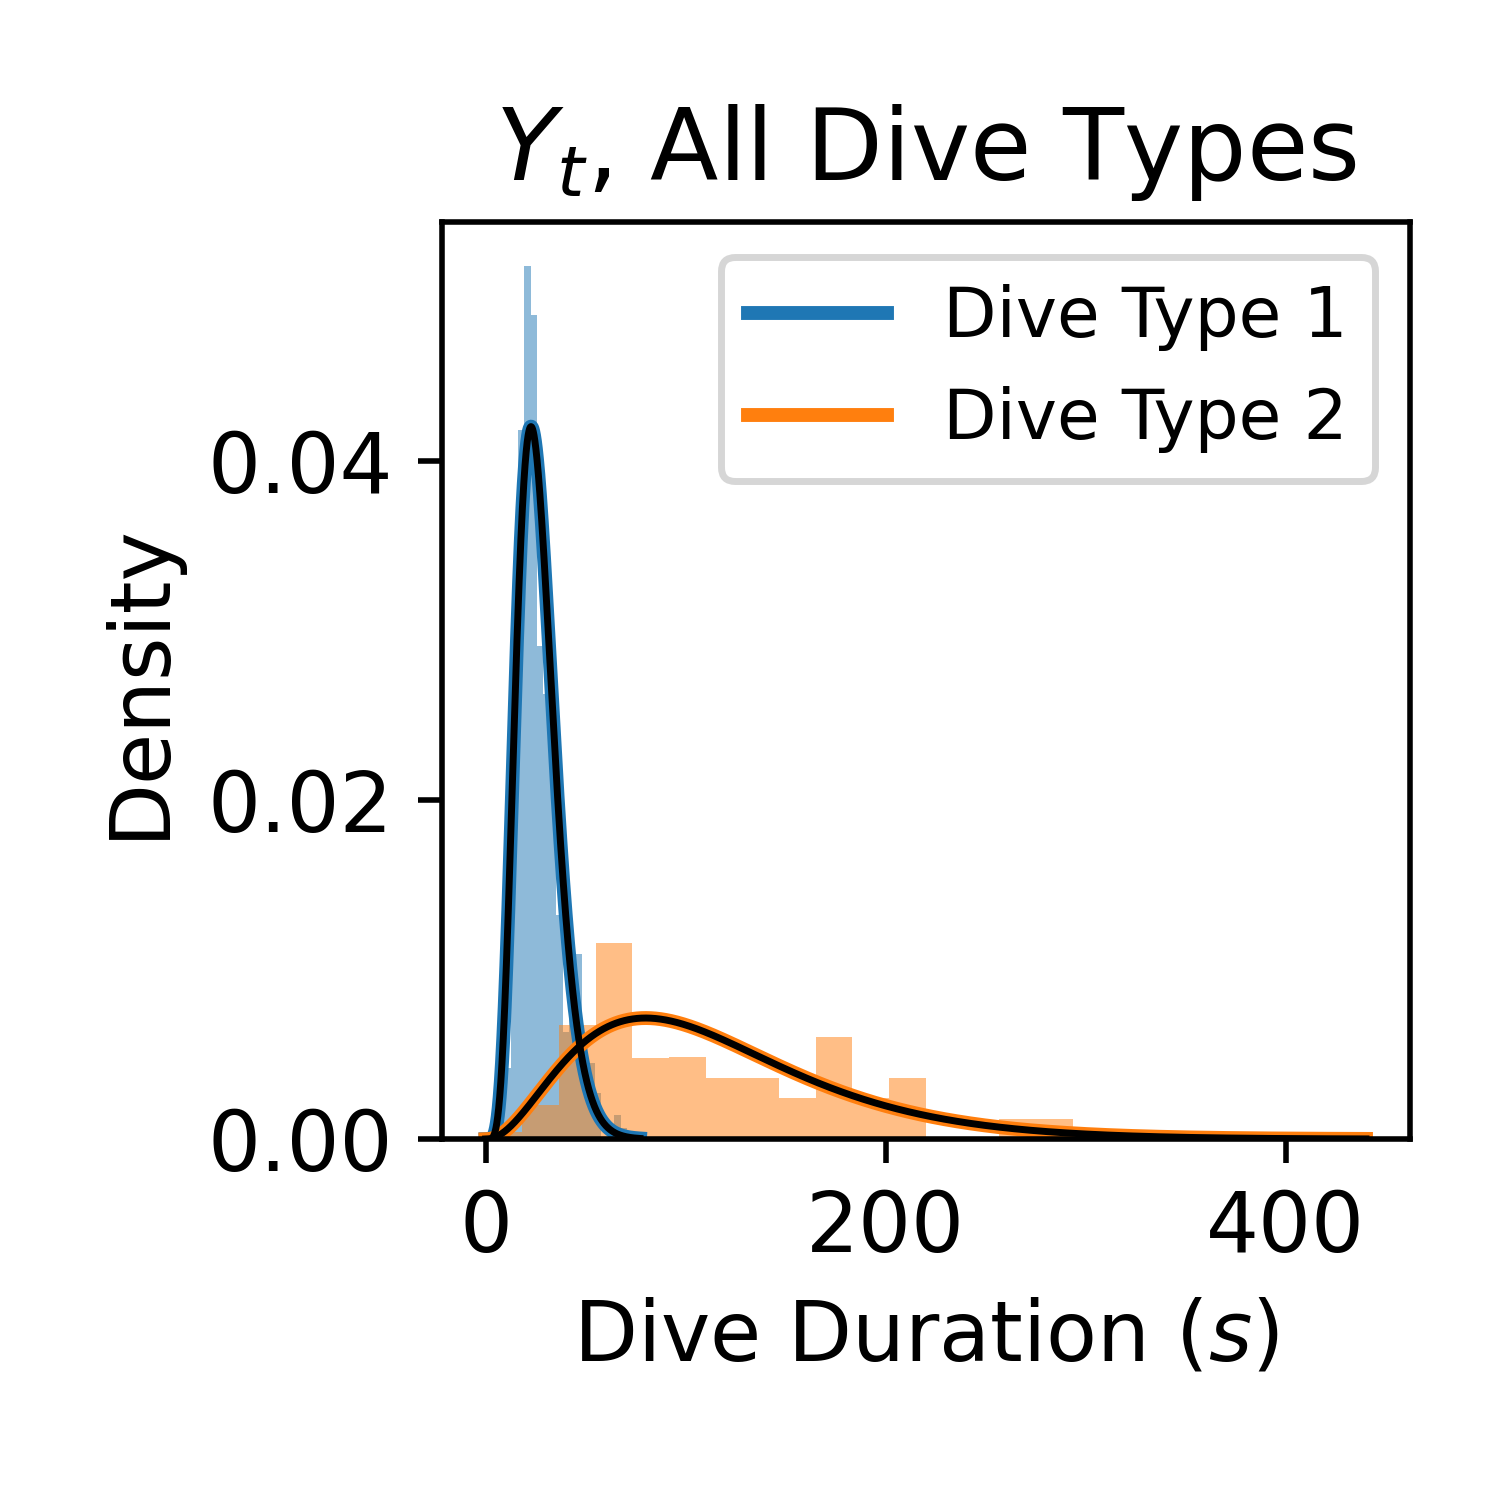
\includegraphics[width=2.25in]{../Plots/2019/20190902-182840-CATs_OB_1_0_267_HHMM_empirical_hist_dive_duration.png}
        \includegraphics[width=2.25in]{../Plots/2019/20190902-182840-CATs_OB_1_0_267_HHMM_pseudresids_Dive_Duration.png}
        \end{center}
        
        \noindent Figure \arabic{fignum}: Empirical histogram (left) and psuedoresiduals (right) of dive duration ($Y_{t}$) plotted over the estimated emission distributions and a standard normal density, respectively. Both plots are generated using the fitted HHMM-DFT and the killer whale case study data.
        \addtocounter{fignum}{1}
        
        \subsection{CarHHMM}
        
        \begin{center}
        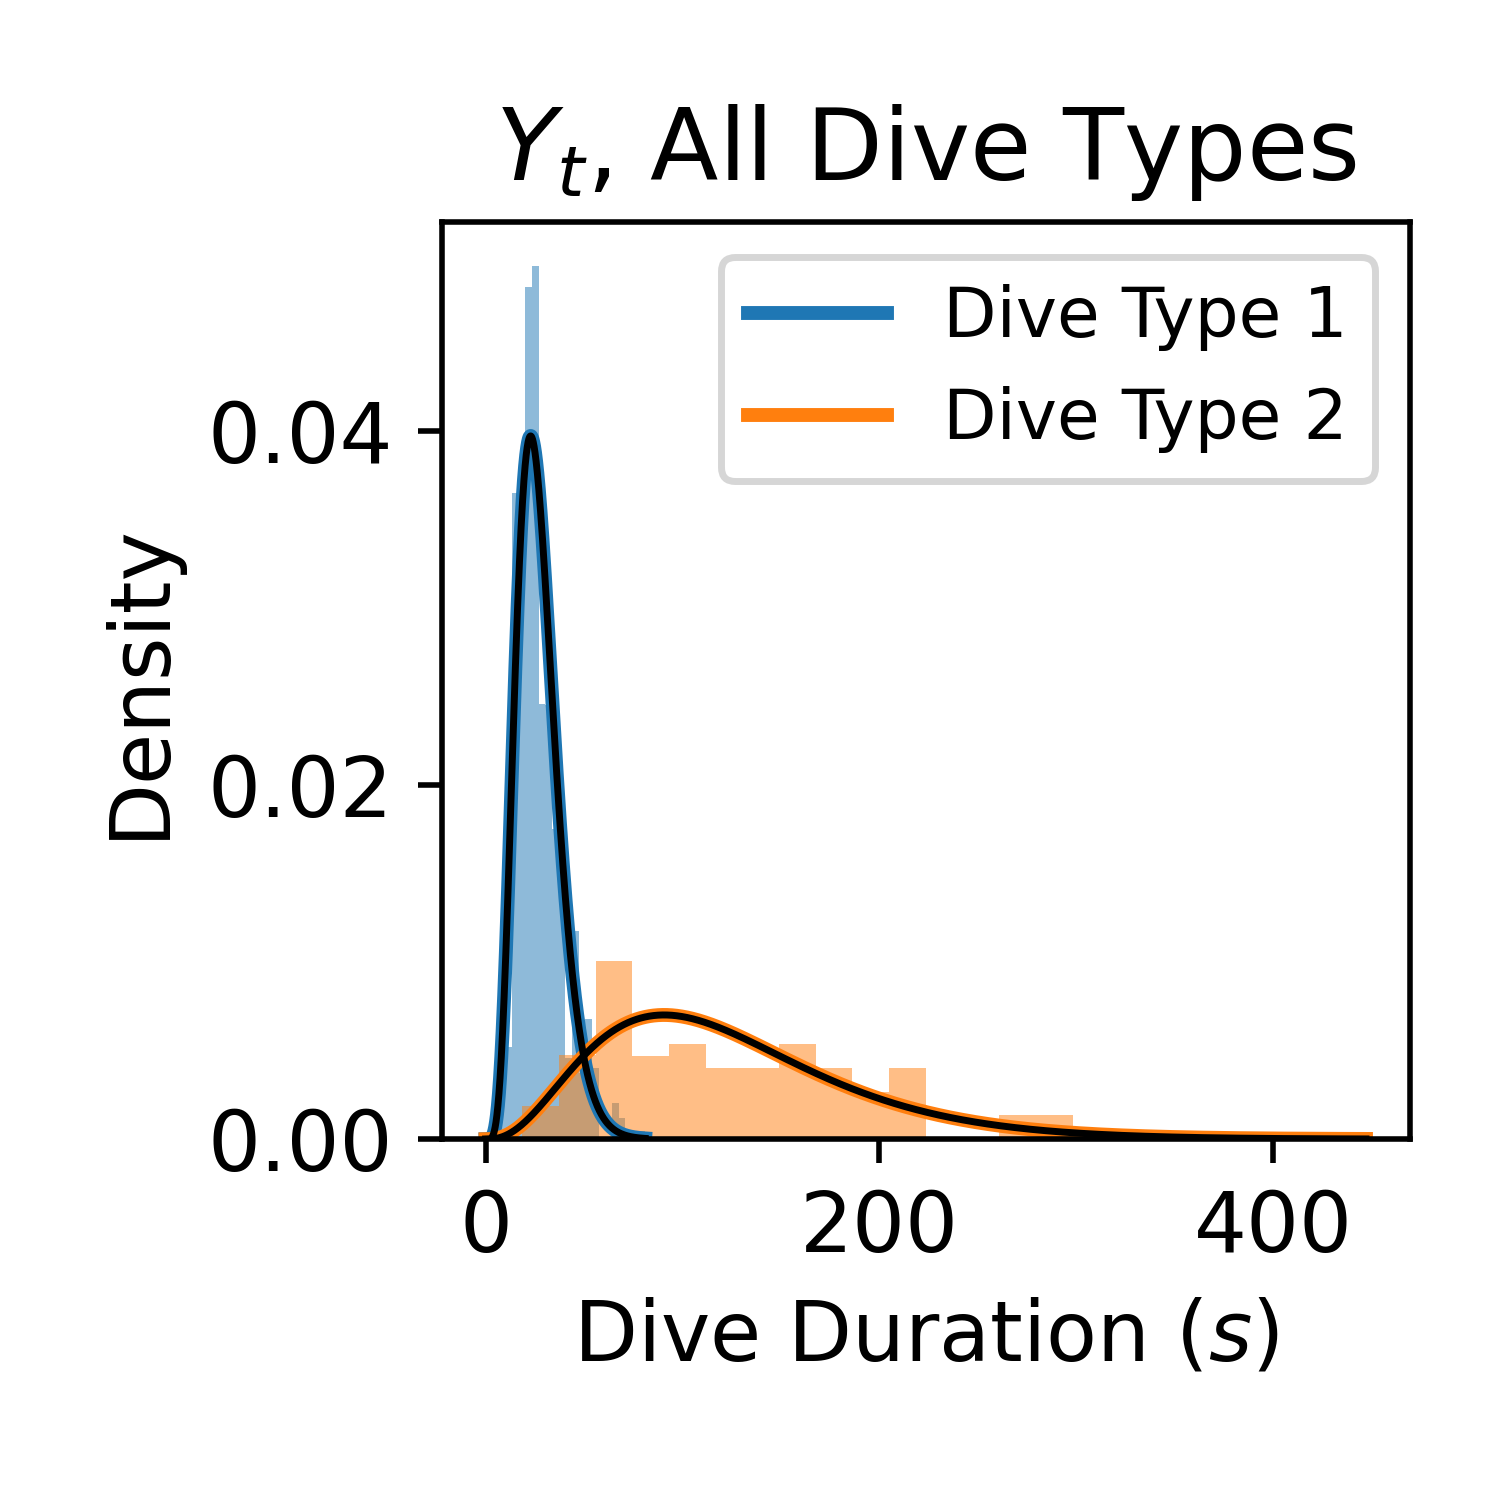
\includegraphics[width=2.25in]{../Plots/2019/20190902-182840-CATs_OB_1_0_267_CarHHMM1_empirical_hist_dive_duration.png}
        \includegraphics[width=2.25in]{../Plots/2019/20190902-182840-CATs_OB_1_0_267_CarHHMM1_pseudresids_Dive_Duration.png}
        \end{center}
        
        \noindent Figure \arabic{fignum}: Empirical histogram (left) and psuedoresiduals (right) of dive duration ($Y_{t}$) plotted over the estimated emission distributions and a standard normal density, respectively. Both plots are generated using the fitted CarHHMM-DFT and the killer whale case study data.
        \addtocounter{fignum}{1}
        
        \subsection{CarHMM-DFT}
        
        \begin{center}
        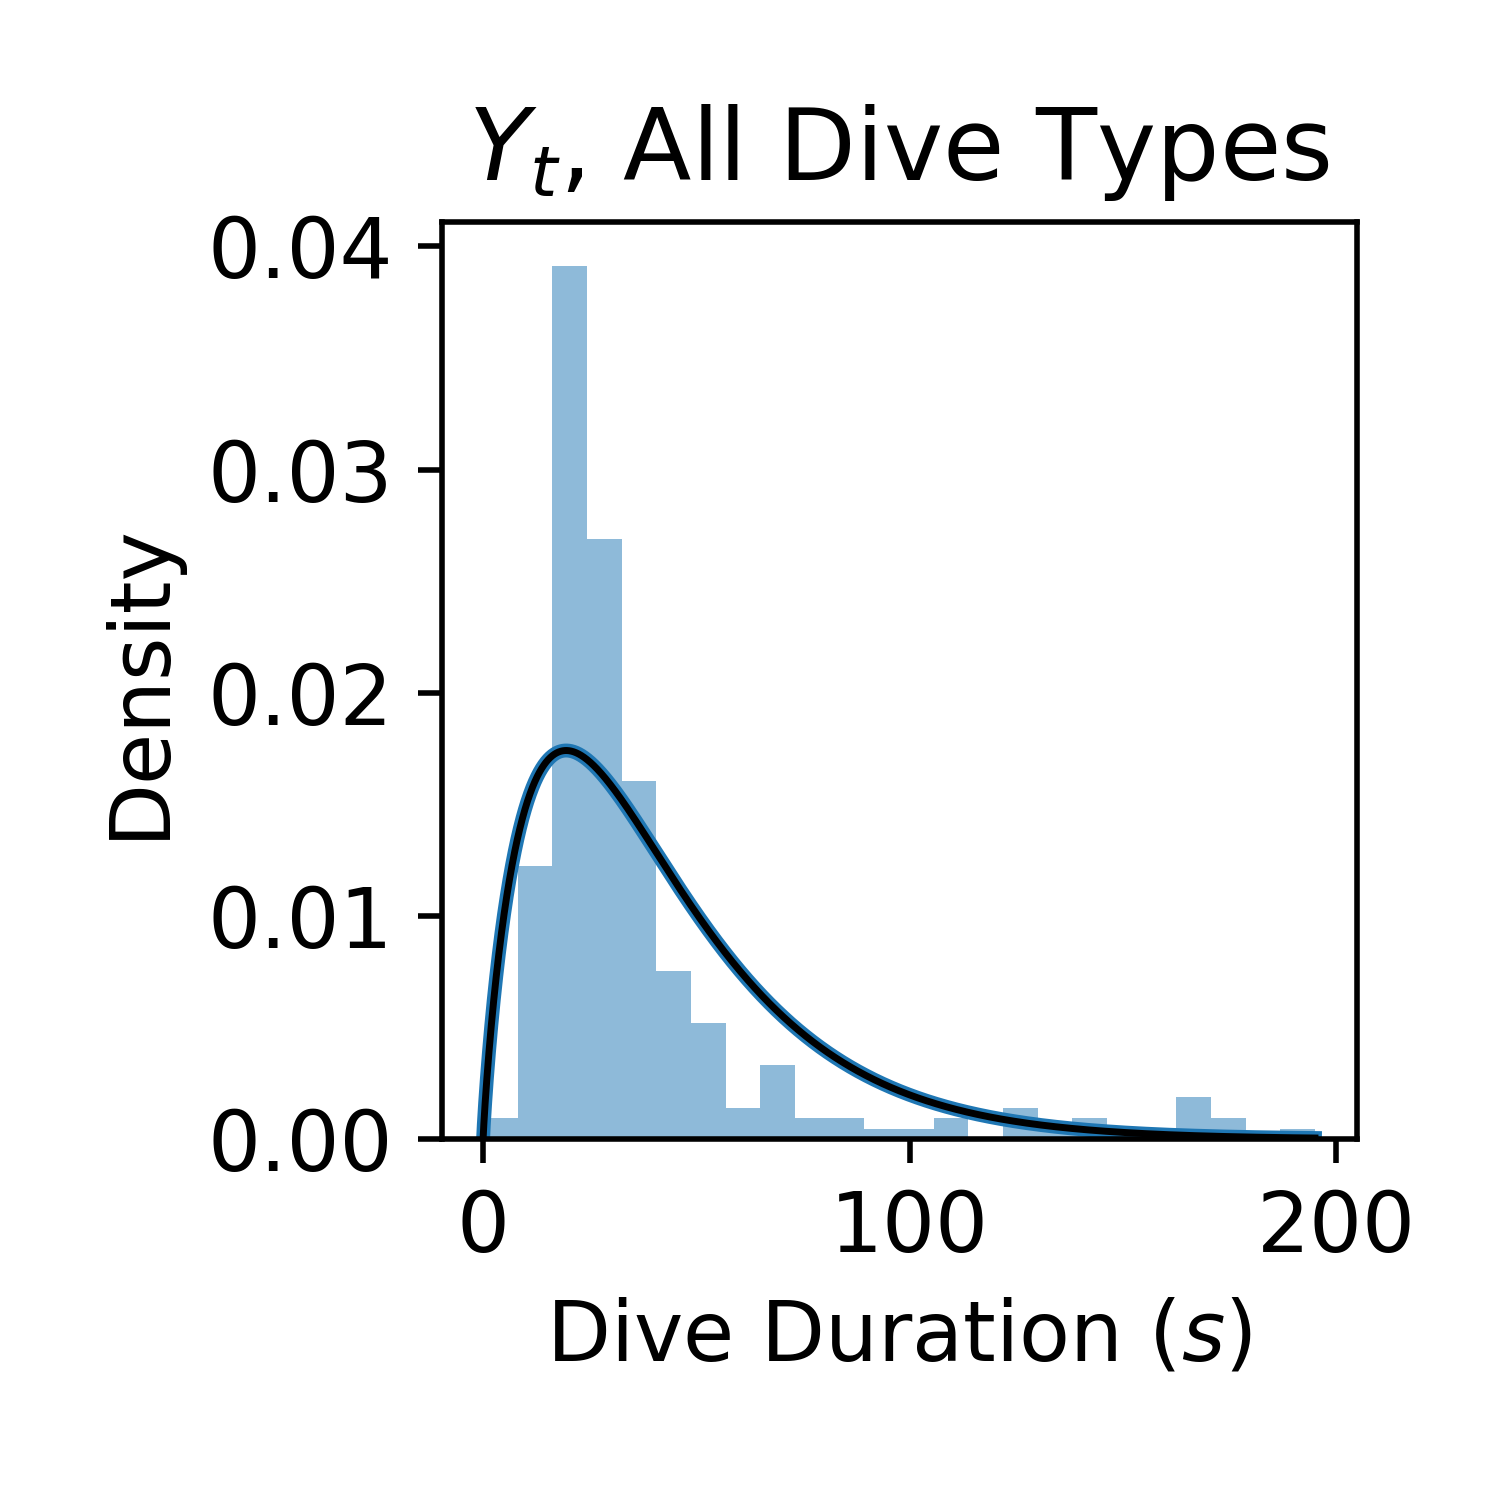
\includegraphics[width=2.25in]{../Plots/2019/20190902-182840-CATs_OB_1_0_267_CarHMM_empirical_hist_dive_duration.png}
        \includegraphics[width=2.25in]{../Plots/2019/20190902-182840-CATs_OB_1_0_267_CarHMM_pseudresids_Dive_Duration.png}
        \end{center}
        
        \noindent Figure \arabic{fignum}: Empirical histogram (left) and psuedoresiduals (right) of dive duration ($Y_{t}$) plotted over the estimated emission distribution (left) and a standard normal density (right), respectively. Both plots are generated using the fitted CarHMM-DFT and the killer whale case study data.
        \addtocounter{fignum}{1}
        
    \newpage
    \section{Model checking - acceleration ($\Zone_{t,\tilde t^*}$)}
        
        \subsection{CarHHMM-DFT}
        
        \begin{center}
        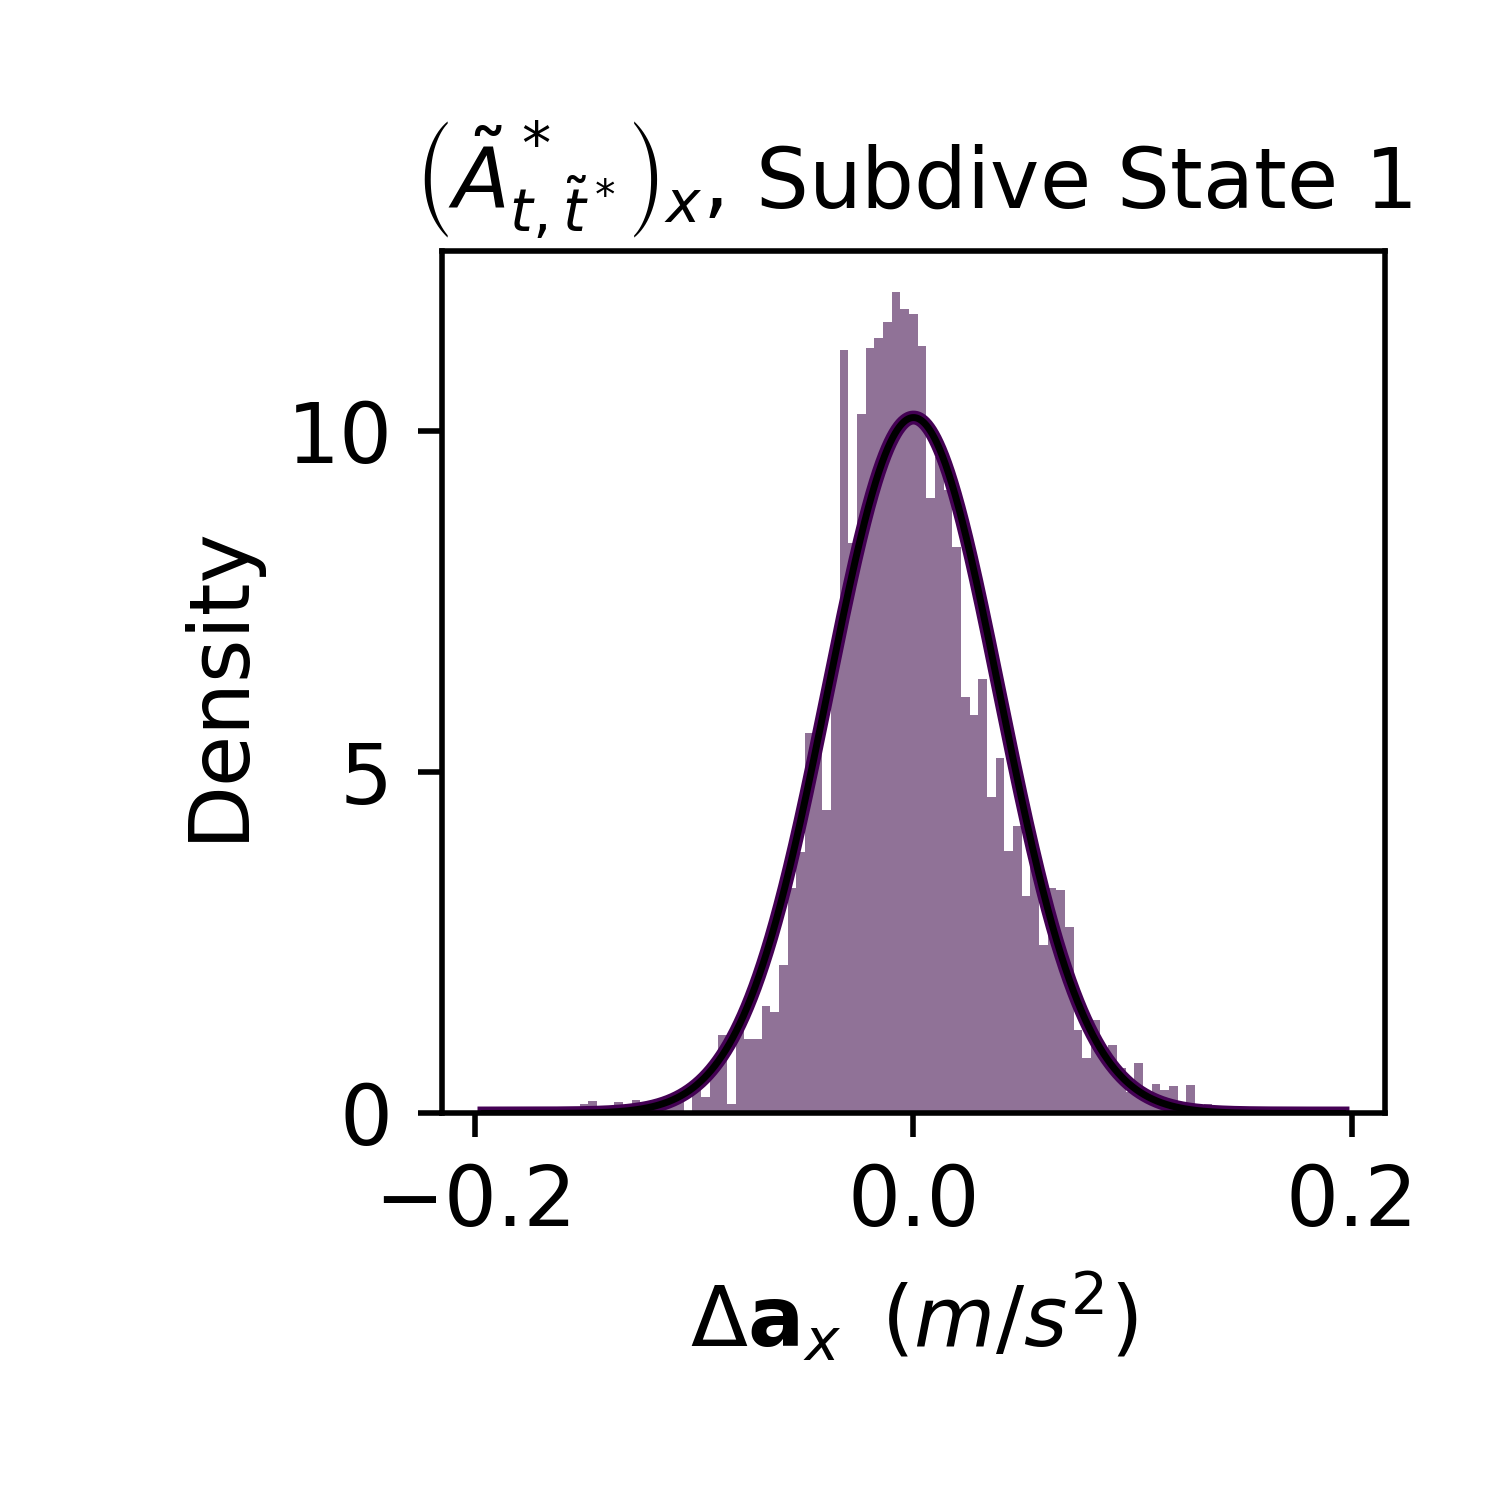
\includegraphics[width=1.75in]{../Plots/2019/20190902-182840-CATs_OB_1_0_267_CarHHMM2_empirical_hist_Ax_0.png}
        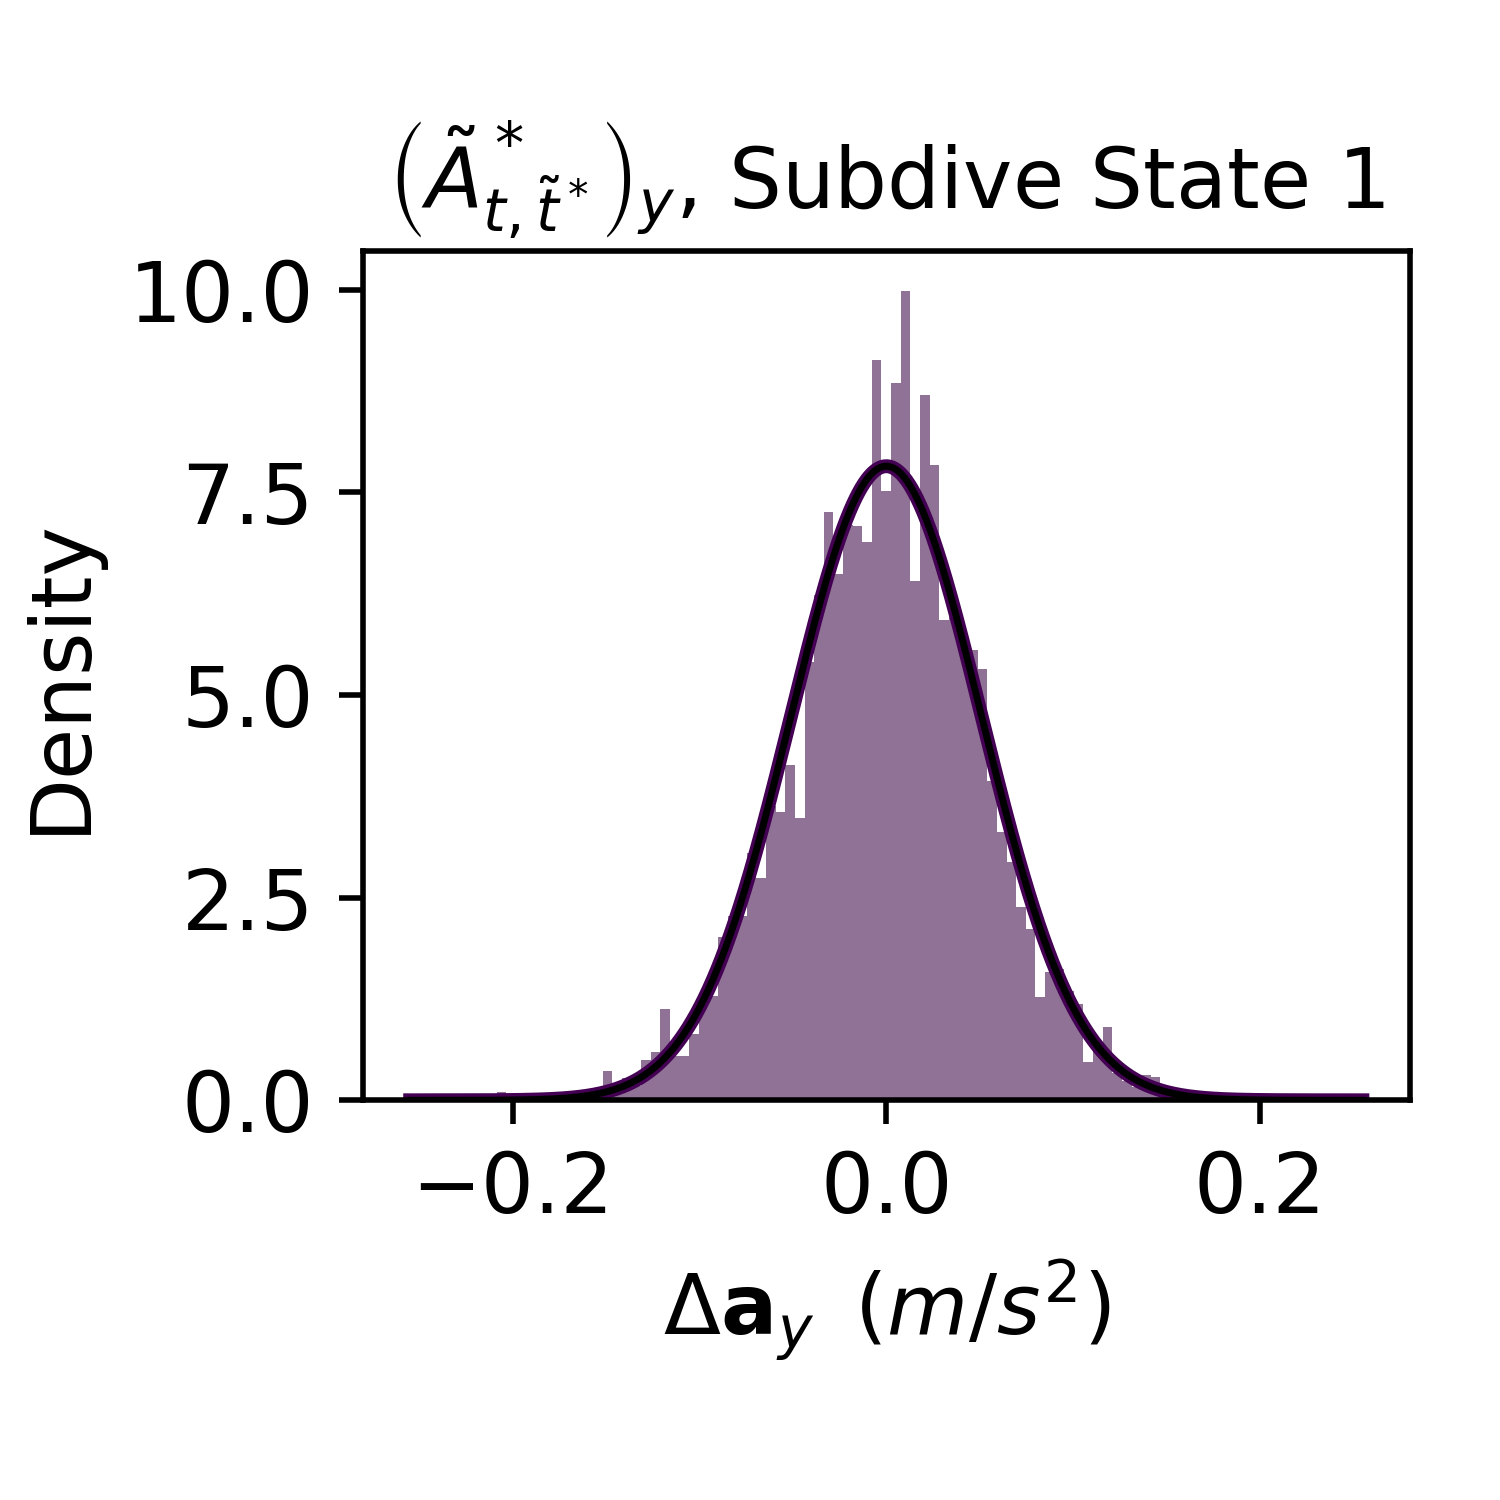
\includegraphics[width=1.75in]{../Plots/2019/20190902-182840-CATs_OB_1_0_267_CarHHMM2_empirical_hist_Ay_0.png}
        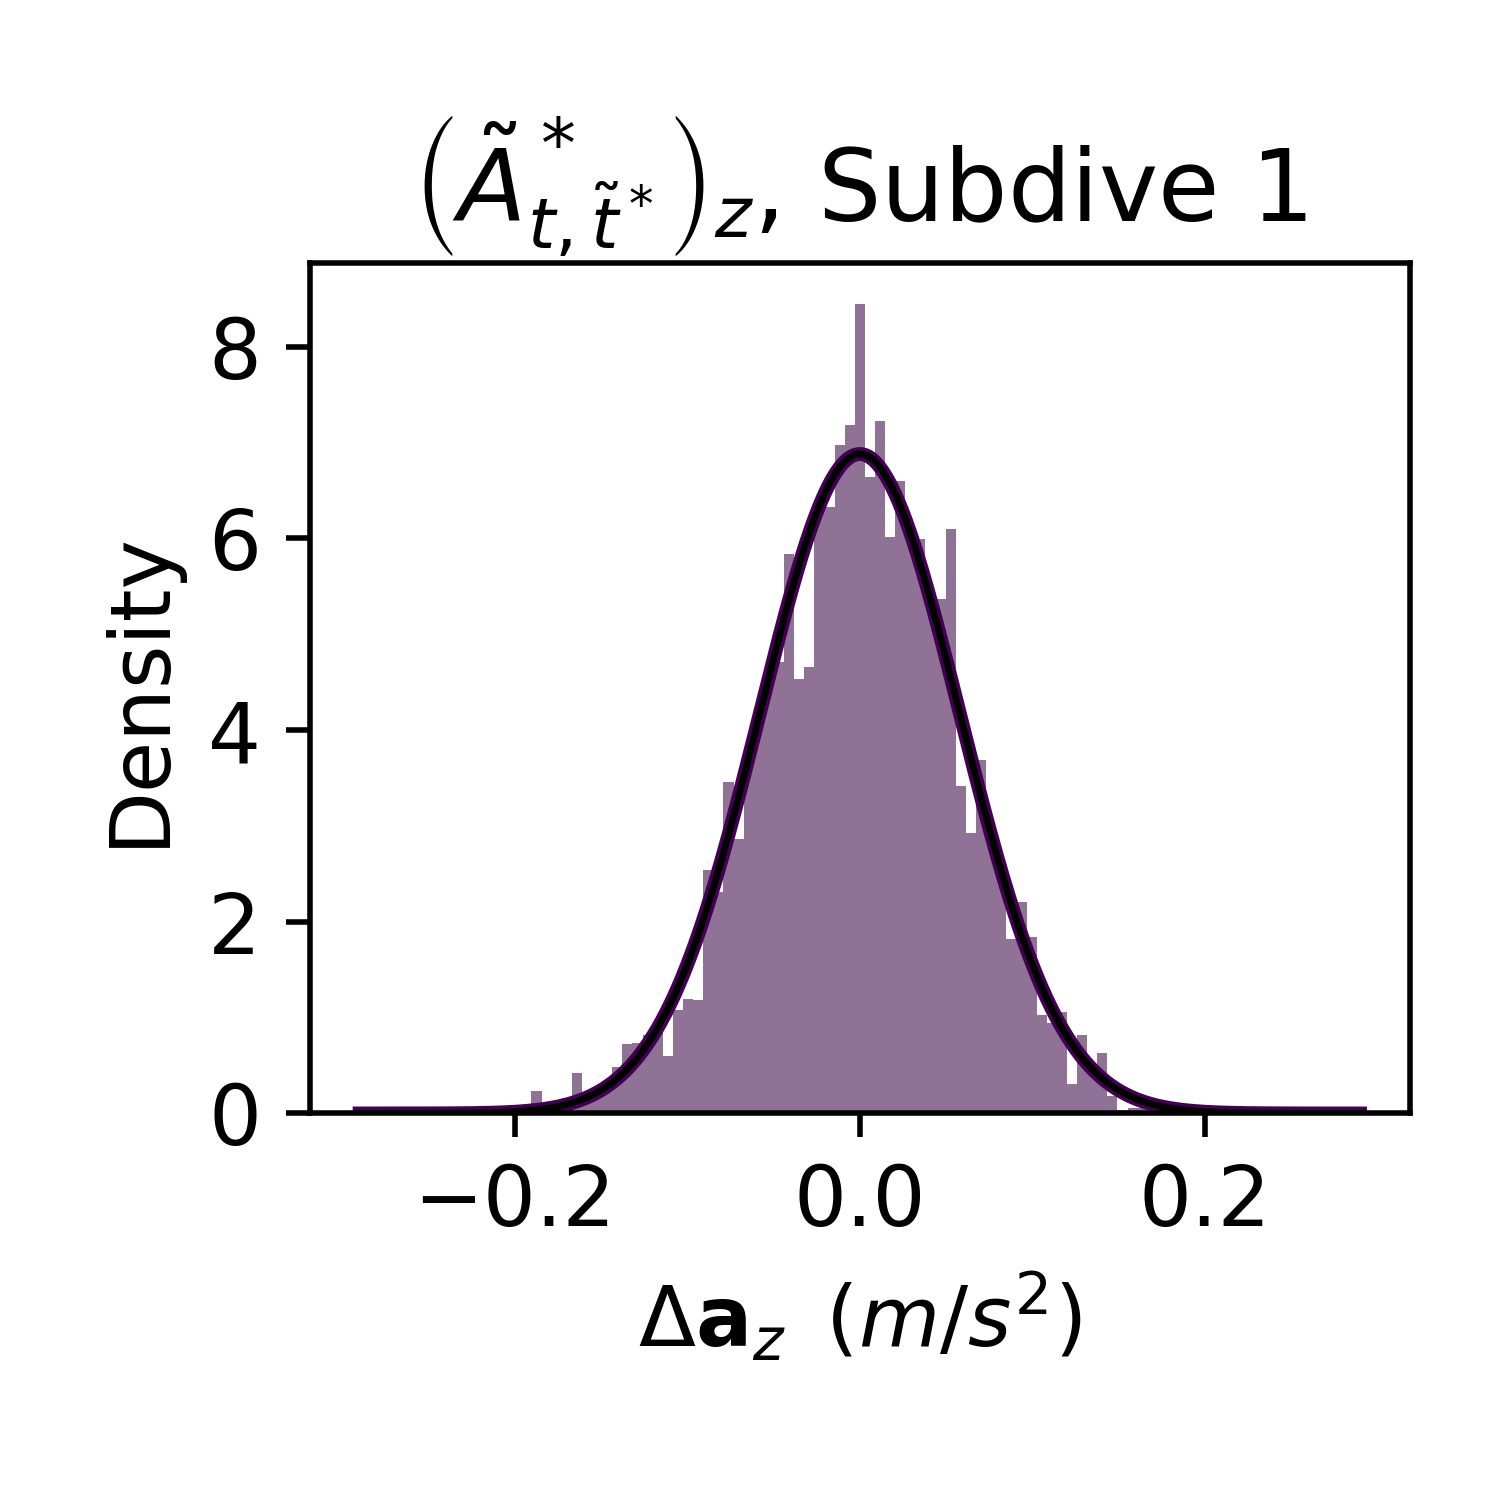
\includegraphics[width=1.75in]{../Plots/2019/20190902-182840-CATs_OB_1_0_267_CarHHMM2_empirical_hist_Az_0.png}
        
        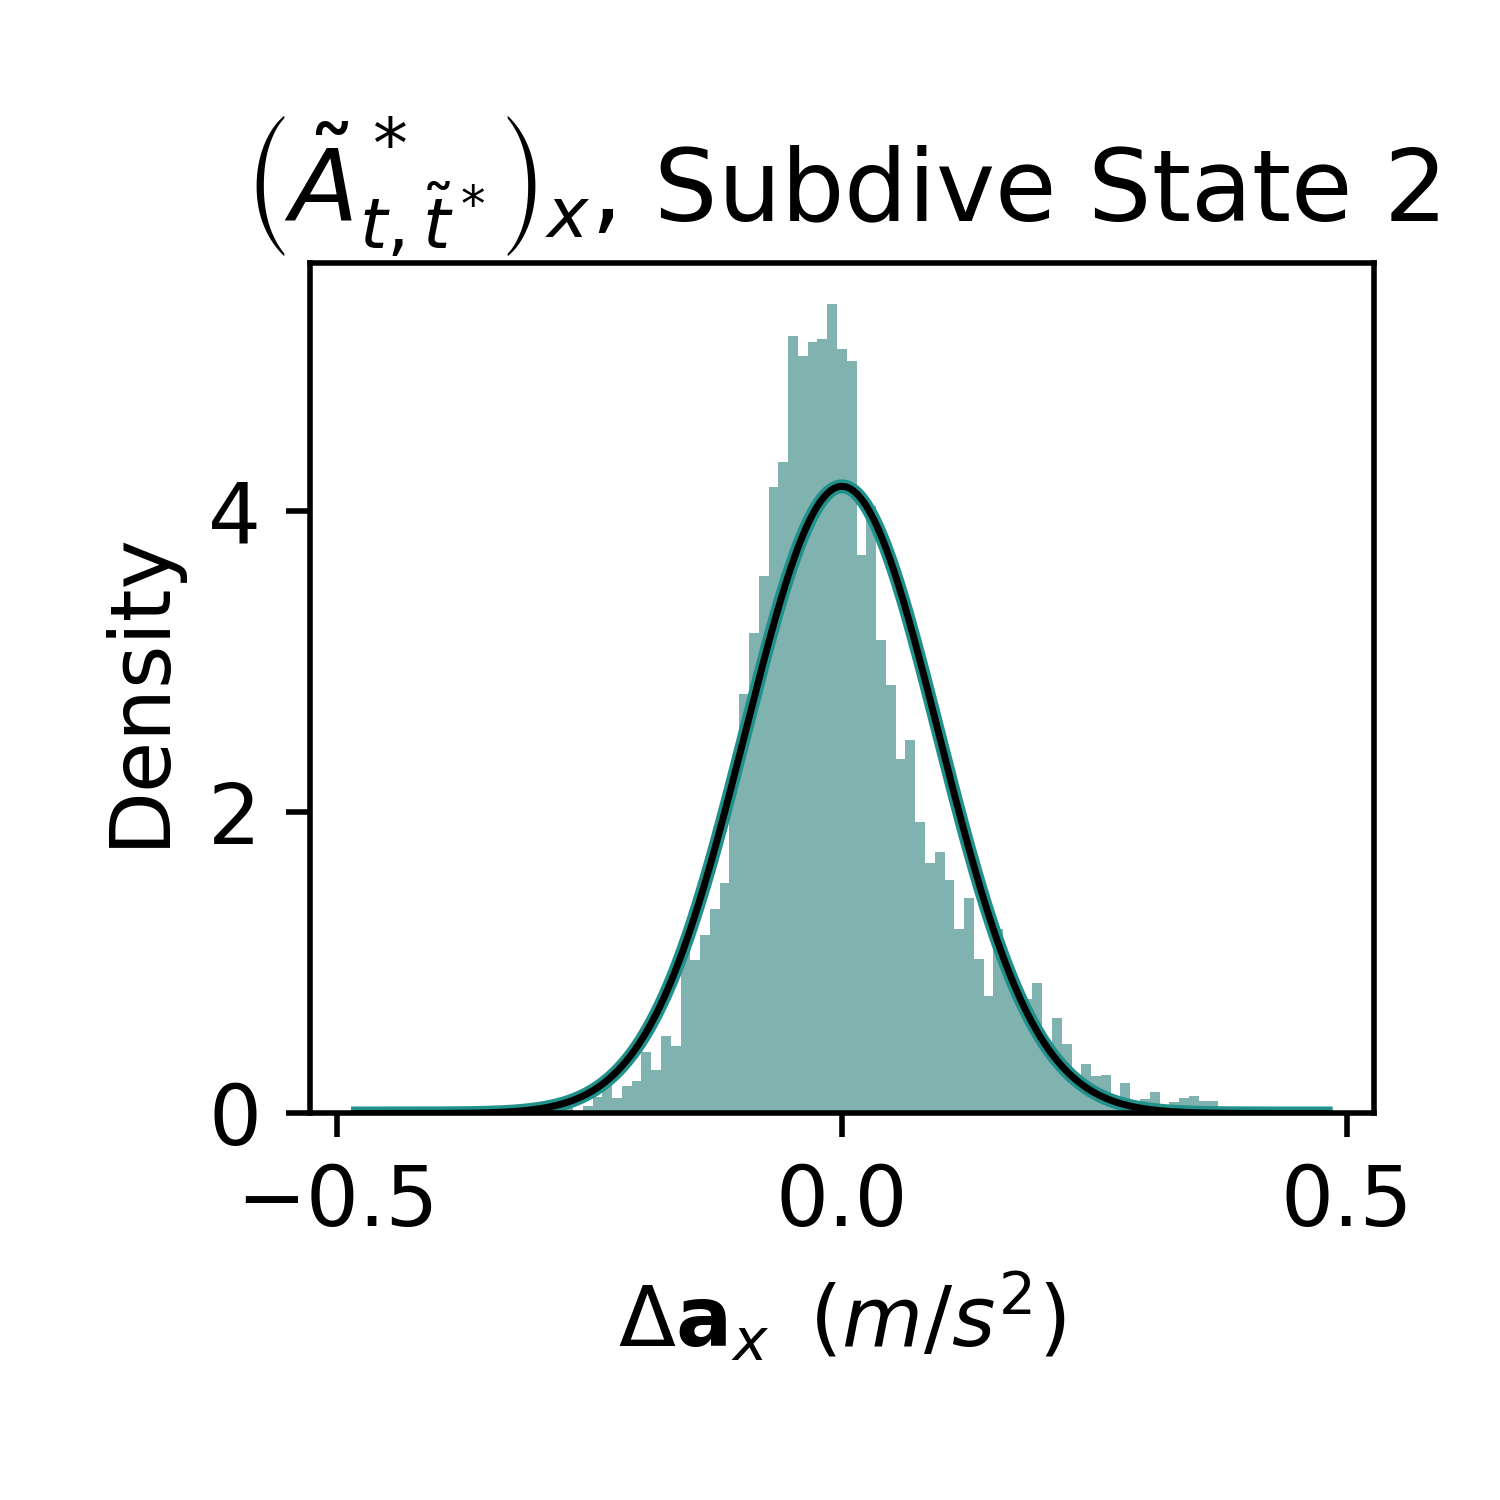
\includegraphics[width=1.75in]{../Plots/2019/20190902-182840-CATs_OB_1_0_267_CarHHMM2_empirical_hist_Ax_1.png}
        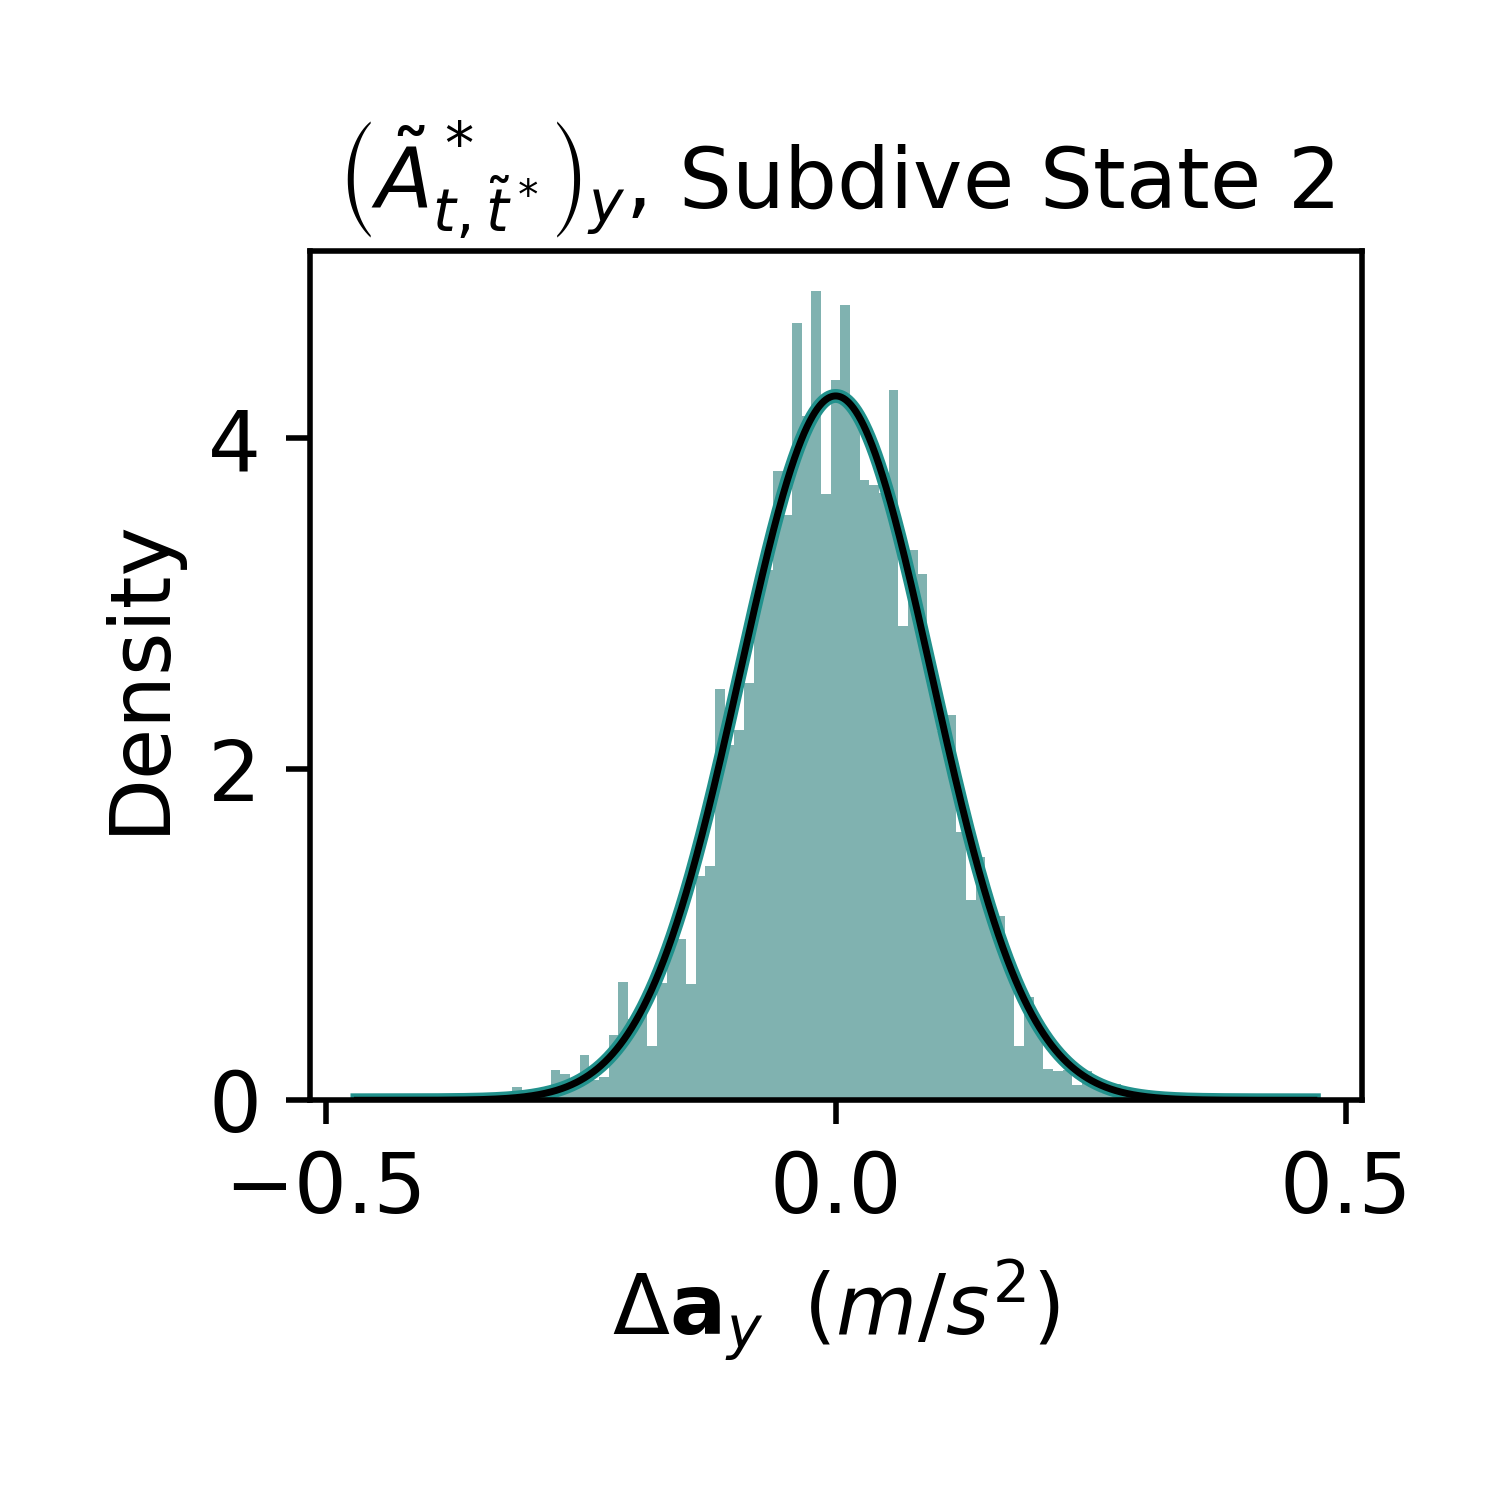
\includegraphics[width=1.75in]{../Plots/2019/20190902-182840-CATs_OB_1_0_267_CarHHMM2_empirical_hist_Ay_1.png}
        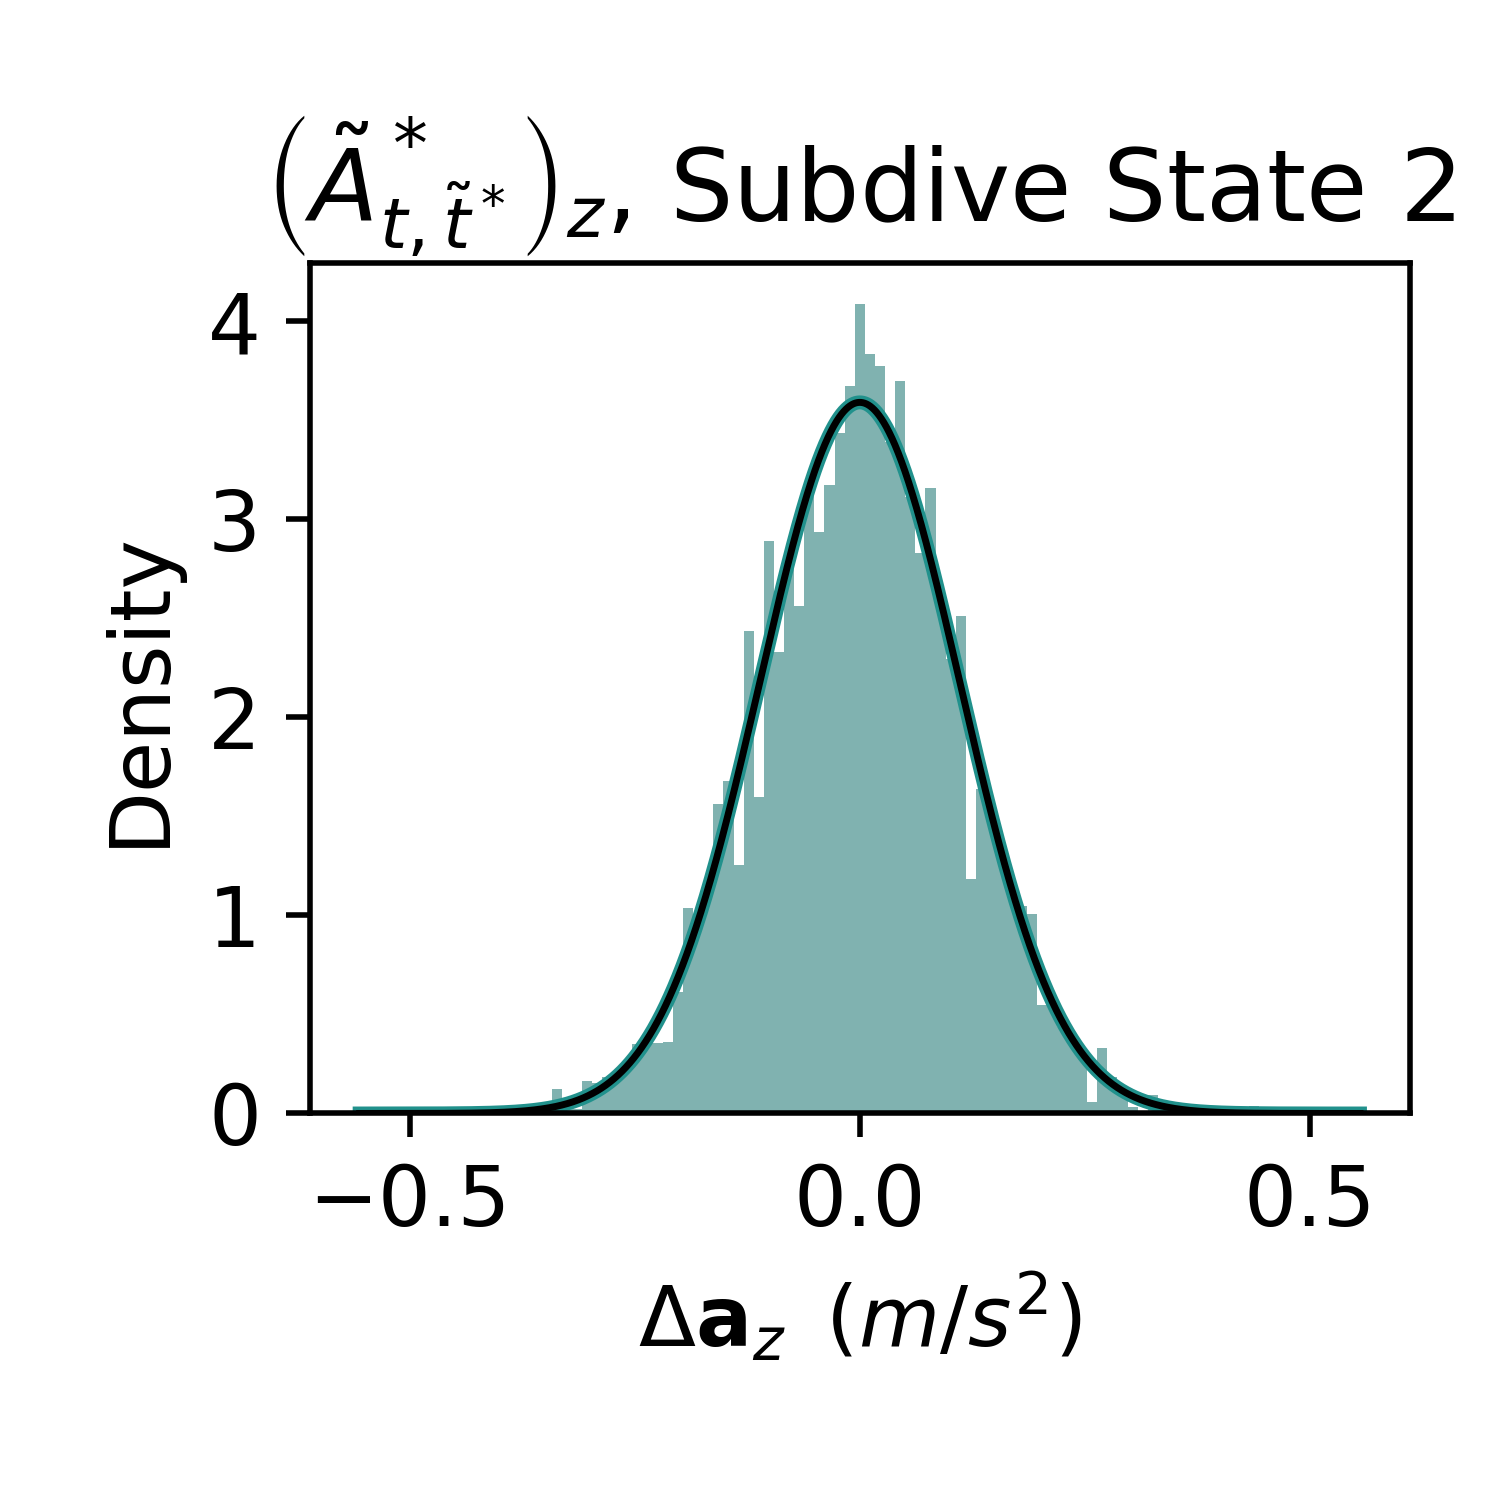
\includegraphics[width=1.75in]{../Plots/2019/20190902-182840-CATs_OB_1_0_267_CarHHMM2_empirical_hist_Az_1.png}
        
        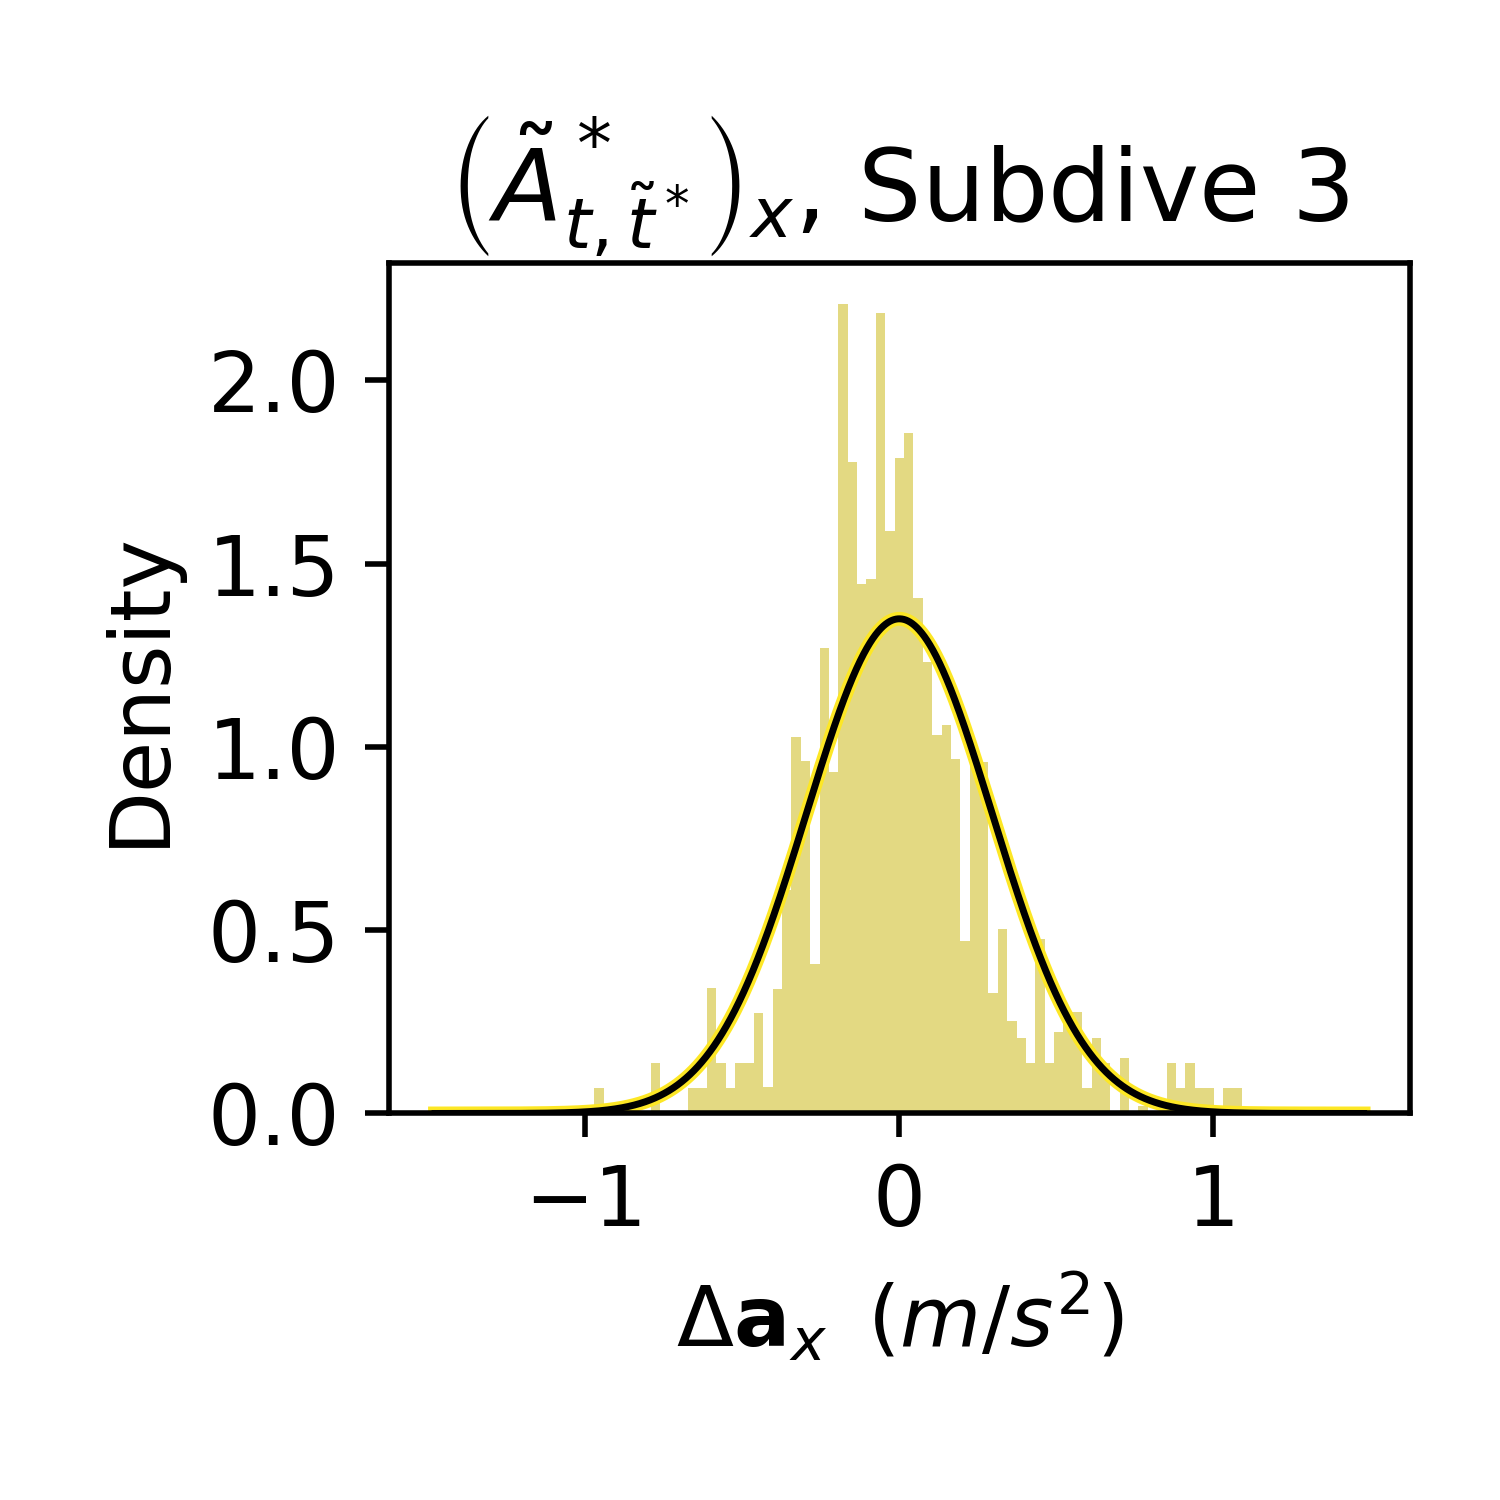
\includegraphics[width=1.75in]{../Plots/2019/20190902-182840-CATs_OB_1_0_267_CarHHMM2_empirical_hist_Ax_2.png}
        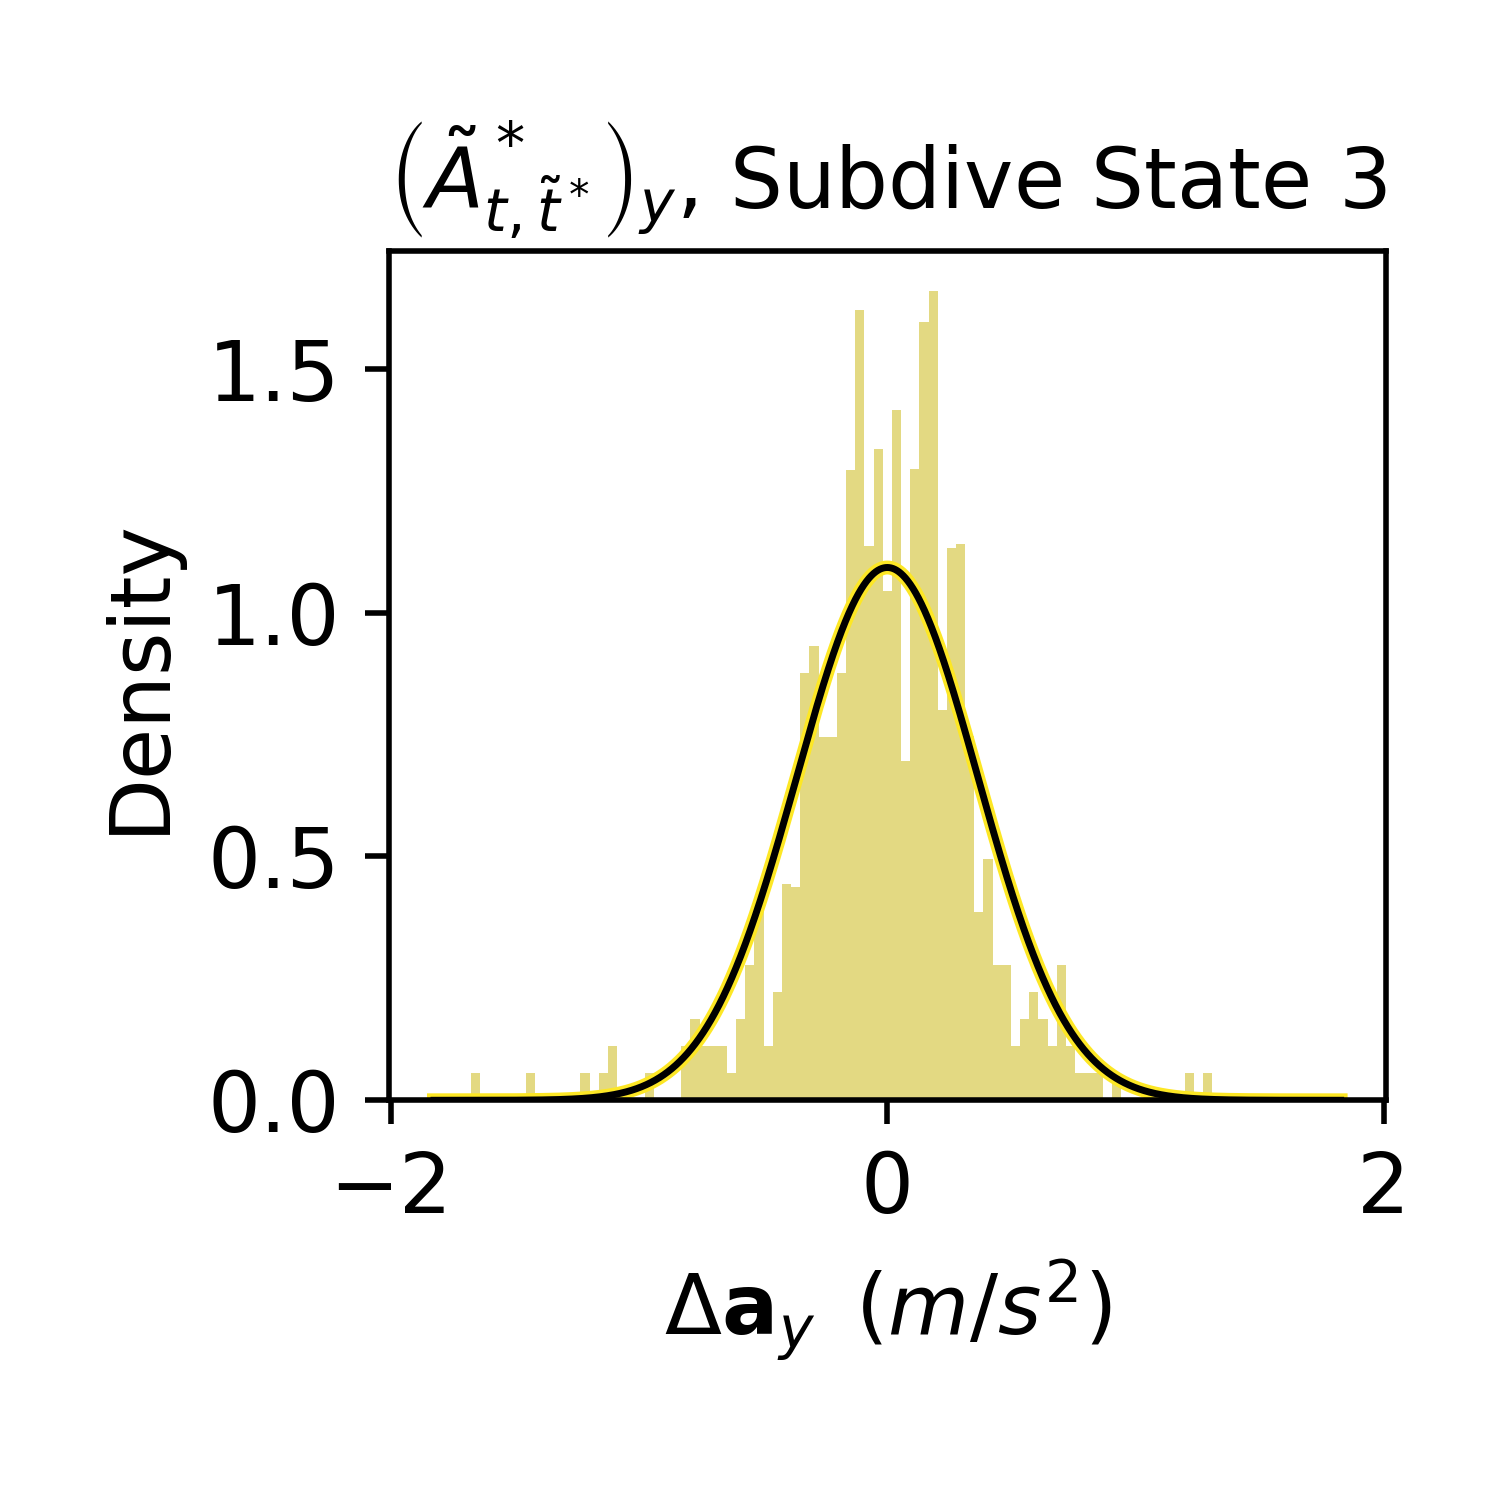
\includegraphics[width=1.75in]{../Plots/2019/20190902-182840-CATs_OB_1_0_267_CarHHMM2_empirical_hist_Ay_2.png}
        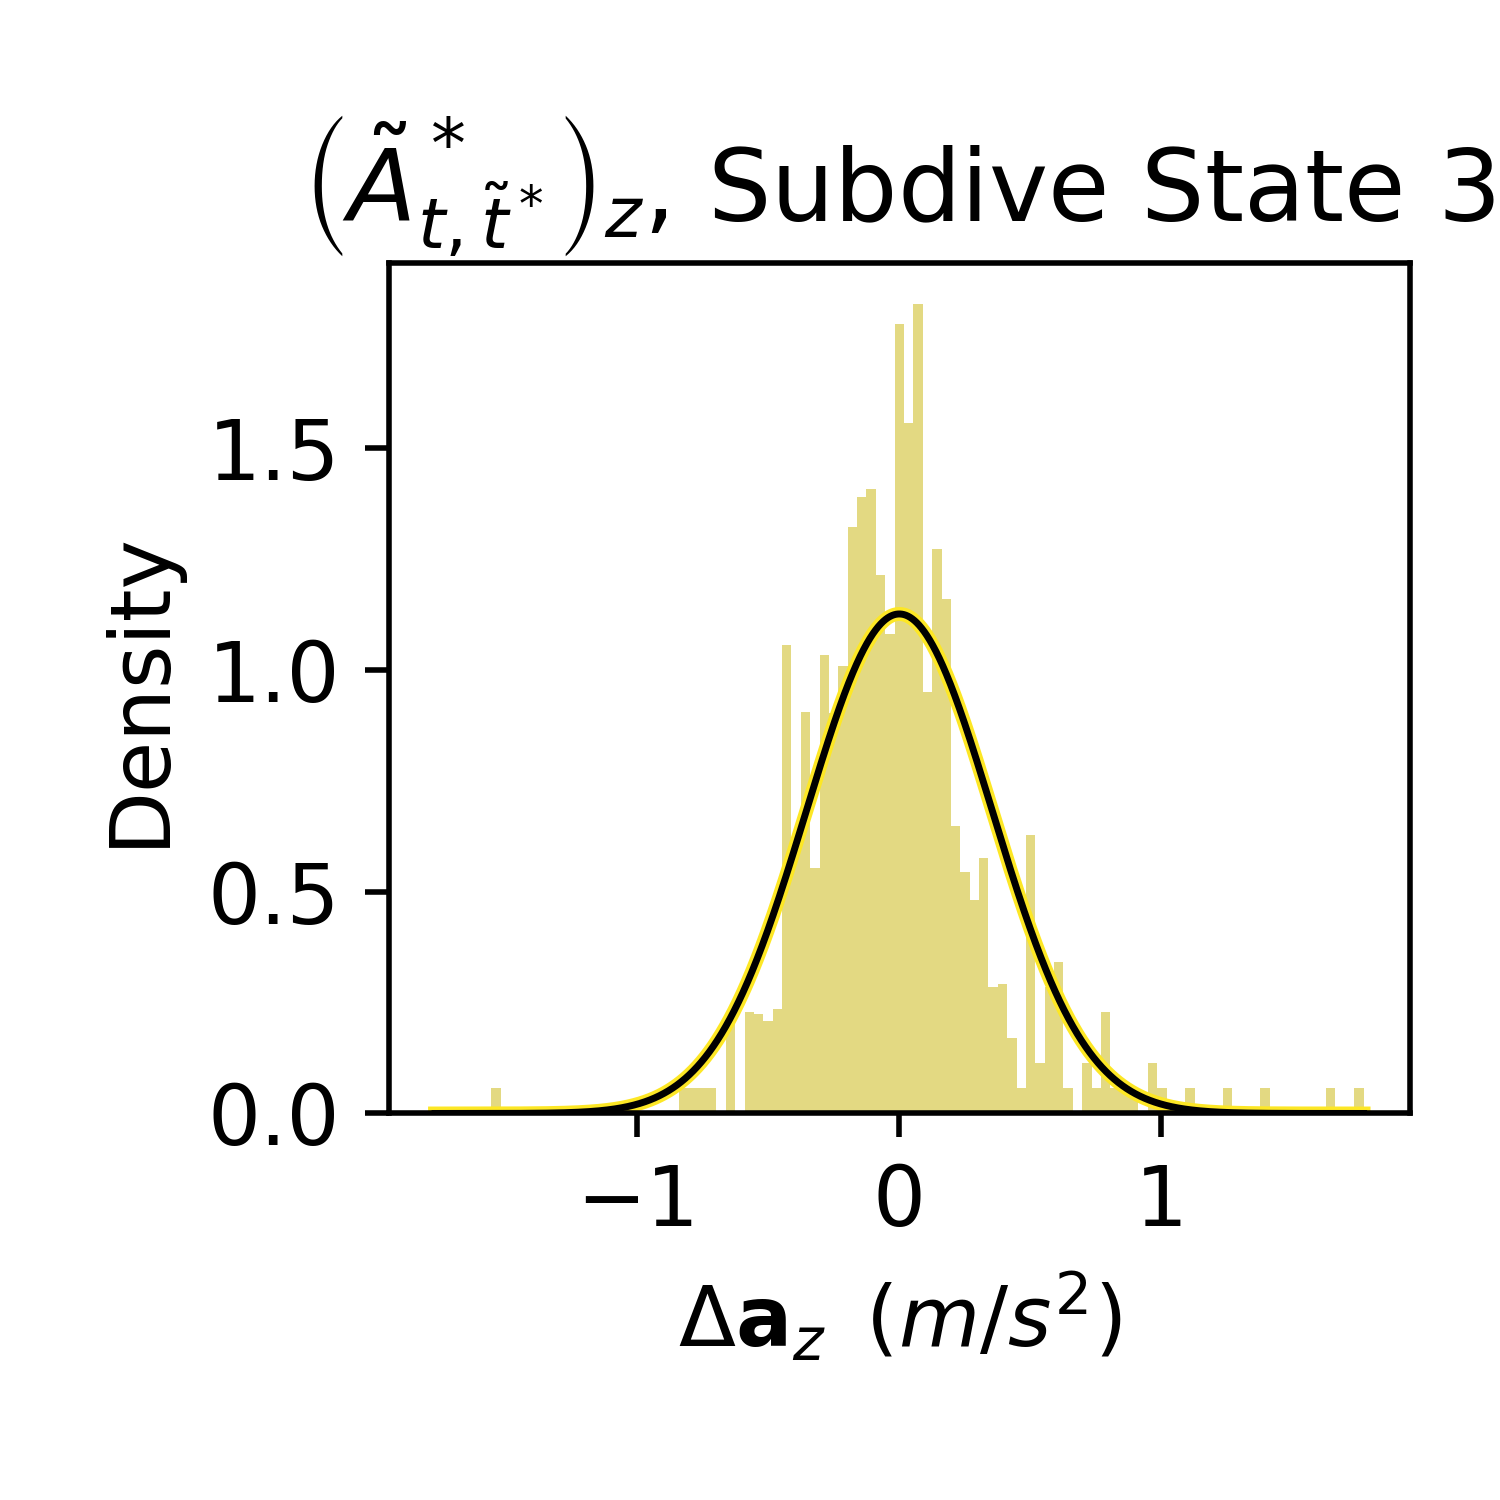
\includegraphics[width=1.75in]{../Plots/2019/20190902-182840-CATs_OB_1_0_267_CarHHMM2_empirical_hist_Az_2.png}
        
        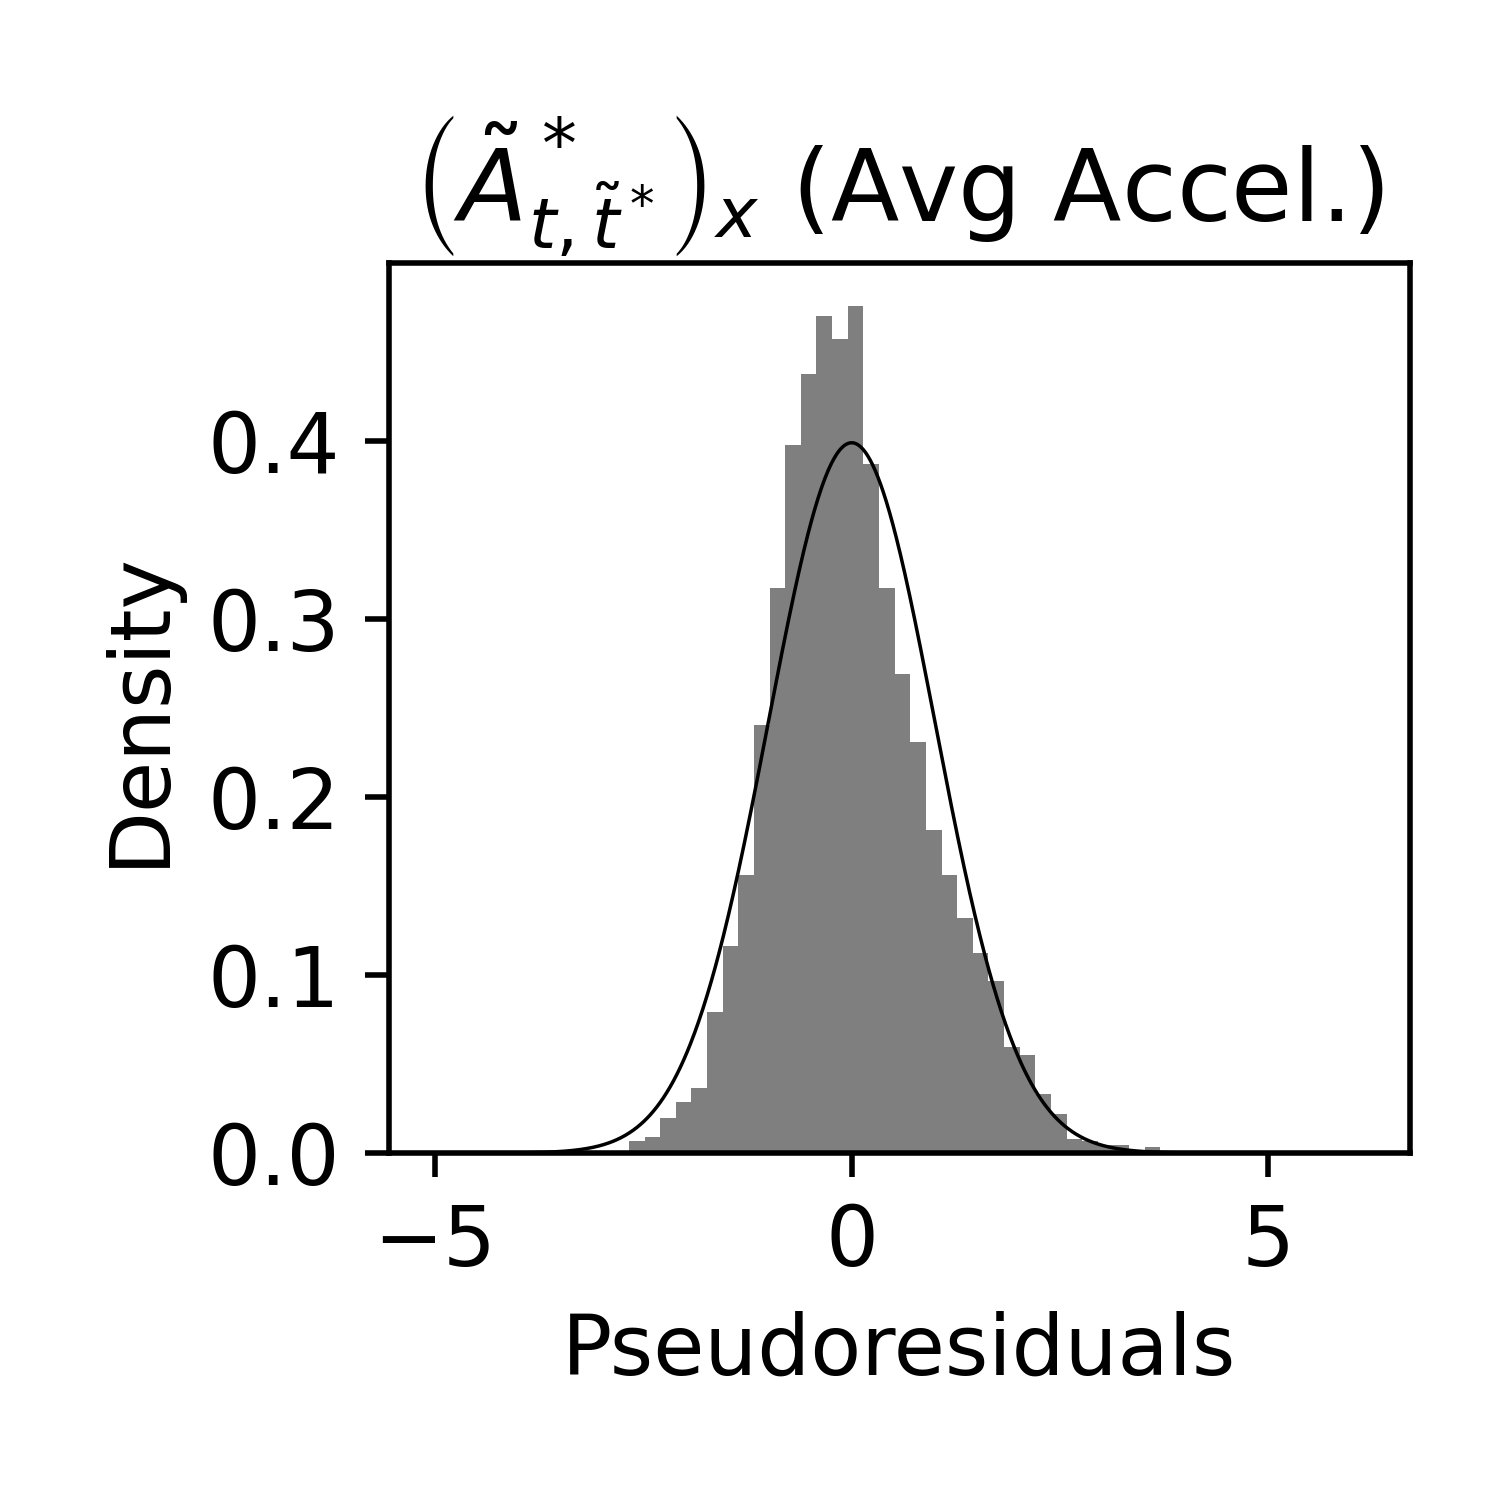
\includegraphics[width=1.75in]{../Plots/2019/20190902-182840-CATs_OB_1_0_267_CarHHMM2_pseudresids_Ax.png}
        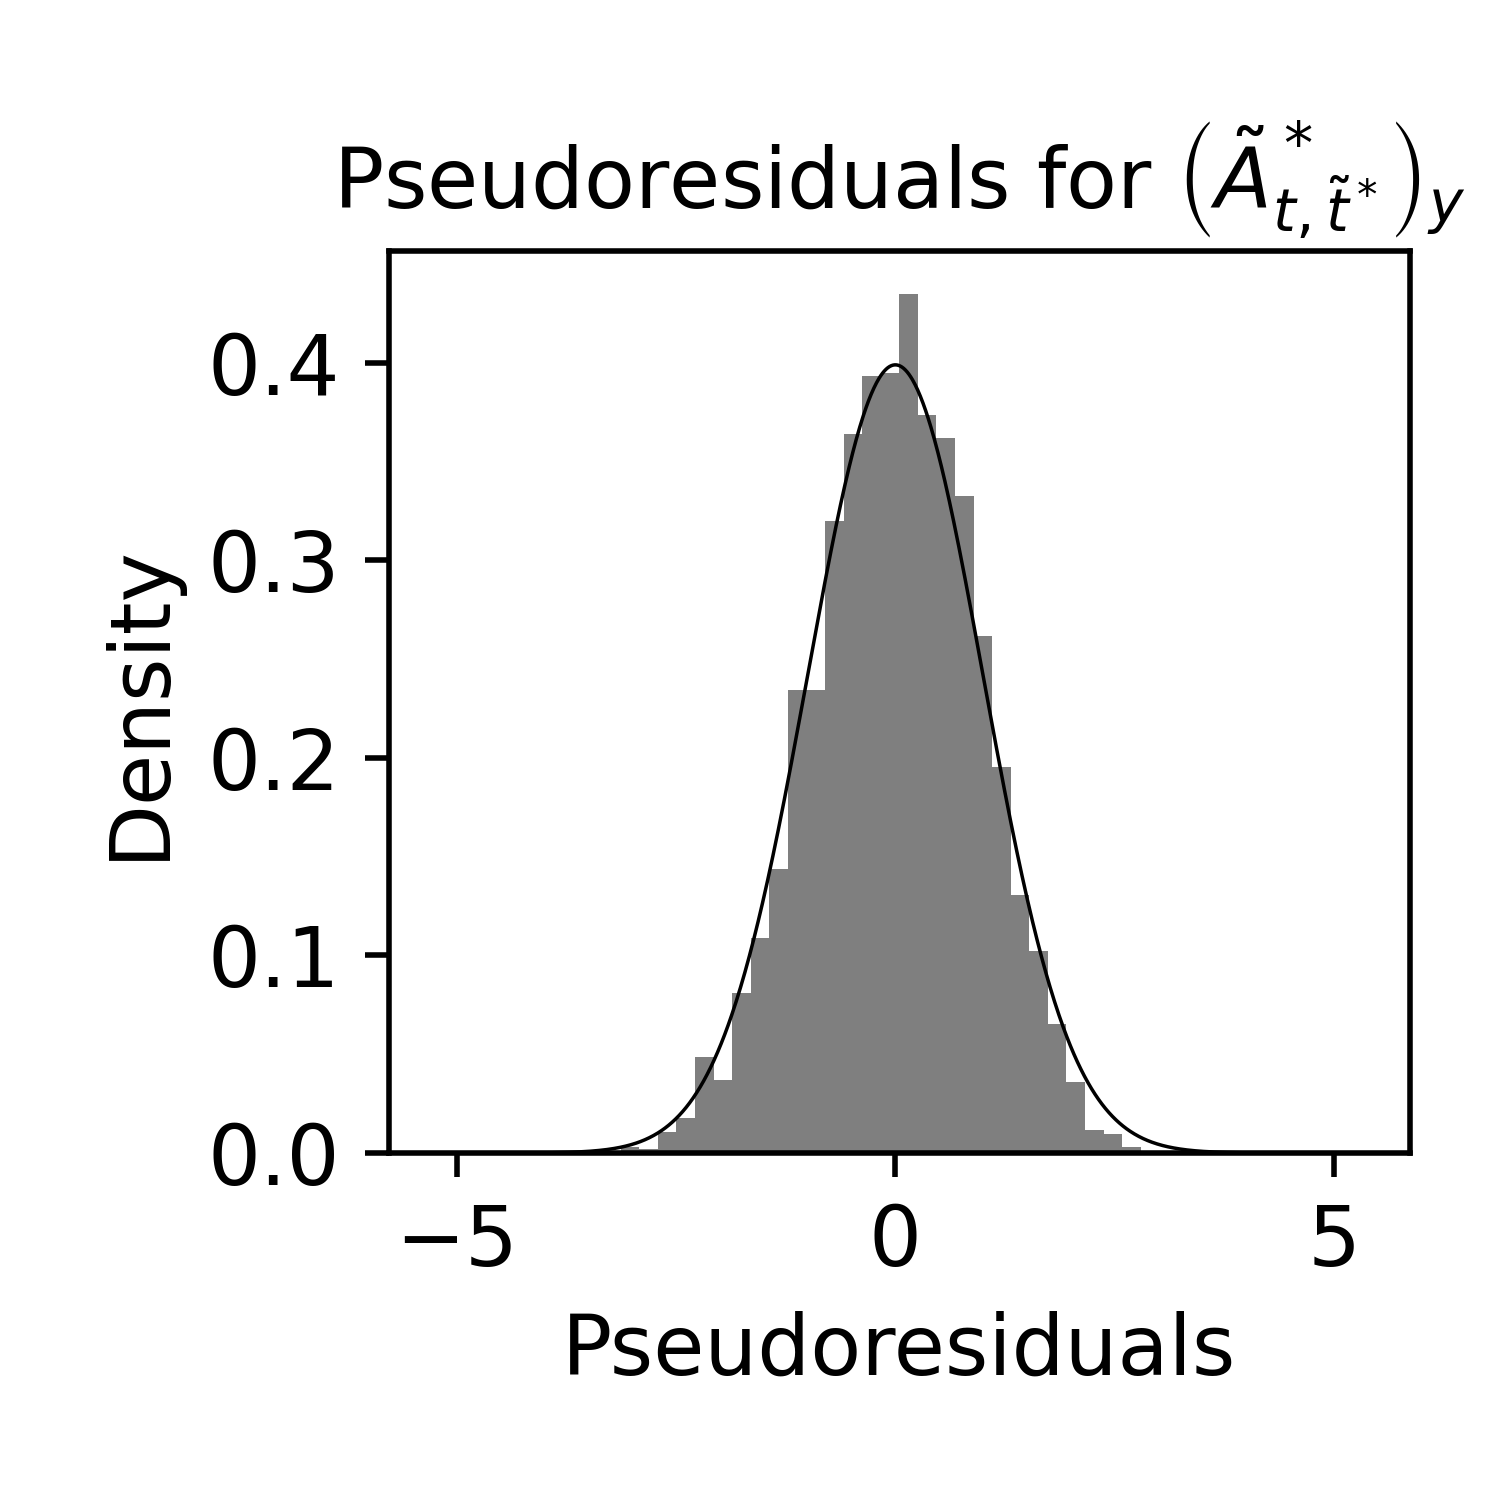
\includegraphics[width=1.75in]{../Plots/2019/20190902-182840-CATs_OB_1_0_267_CarHHMM2_pseudresids_Ay.png}
        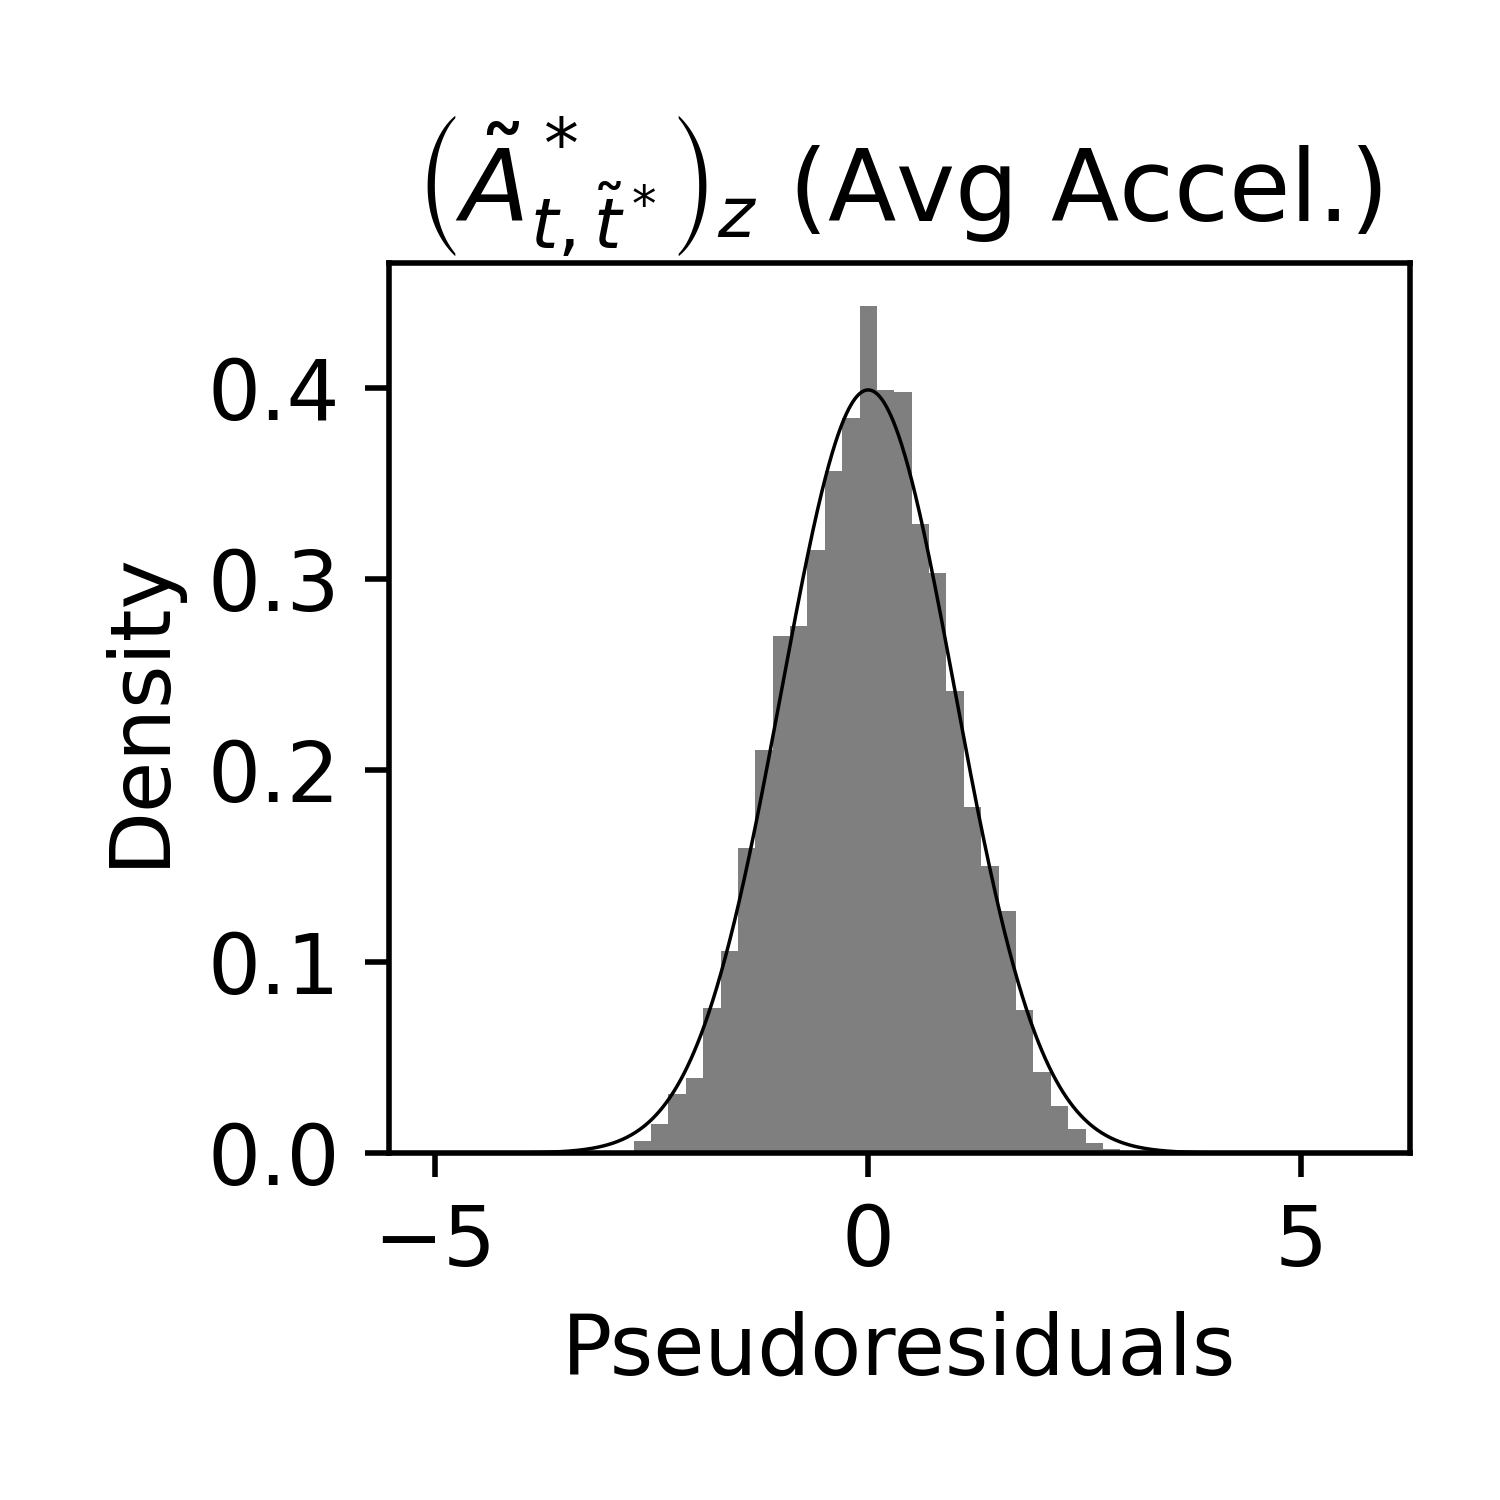
\includegraphics[width=1.75in]{../Plots/2019/20190902-182840-CATs_OB_1_0_267_CarHHMM2_pseudresids_Az.png}
        \end{center}
        
        \noindent Figure \arabic{fignum}: Empirical histograms (top three rows) and psuedoresiduals (bottom row) of acceleration ($\Zone_{t,\tilde t^*}$) plotted over the estimated emission distributions and a standard normal density, respectively. Note that the mean of acceleration at time $\tilde t^*$ depends upon acceleration at time $\tilde t^*-1$, so only the deviation from the conditional mean at each particular time step is plotted. All plots are generated using the fitted CarHHMM-DFT and the killer whale case study data.
        \addtocounter{fignum}{1}
        
        \newpage
        
        \subsection{HHMM-DFT}
        
        \begin{center}
        \includegraphics[width=1.75in]{../Plots/2019/20190902-182840-CATs_OB_1_0_267_HHMM_empirical_hist_Ax_0.png}
        \includegraphics[width=1.75in]{../Plots/2019/20190902-182840-CATs_OB_1_0_267_HHMM_empirical_hist_Ay_0.png}
        \includegraphics[width=1.75in]{../Plots/2019/20190902-182840-CATs_OB_1_0_267_HHMM_empirical_hist_Az_0.png}
        
        \includegraphics[width=1.75in]{../Plots/2019/20190902-182840-CATs_OB_1_0_267_HHMM_empirical_hist_Ax_1.png}
        \includegraphics[width=1.75in]{../Plots/2019/20190902-182840-CATs_OB_1_0_267_HHMM_empirical_hist_Ay_1.png}
        \includegraphics[width=1.75in]{../Plots/2019/20190902-182840-CATs_OB_1_0_267_HHMM_empirical_hist_Az_1.png}
        
        \includegraphics[width=1.75in]{../Plots/2019/20190902-182840-CATs_OB_1_0_267_HHMM_empirical_hist_Ax_2.png}
        \includegraphics[width=1.75in]{../Plots/2019/20190902-182840-CATs_OB_1_0_267_HHMM_empirical_hist_Ay_2.png}
        \includegraphics[width=1.75in]{../Plots/2019/20190902-182840-CATs_OB_1_0_267_HHMM_empirical_hist_Az_2.png}
        
        \includegraphics[width=1.75in]{../Plots/2019/20190902-182840-CATs_OB_1_0_267_HHMM_pseudresids_Ax.png}
        \includegraphics[width=1.75in]{../Plots/2019/20190902-182840-CATs_OB_1_0_267_HHMM_pseudresids_Ay.png}
        \includegraphics[width=1.75in]{../Plots/2019/20190902-182840-CATs_OB_1_0_267_HHMM_pseudresids_Az.png}
        \end{center}
        
        \noindent Figure \arabic{fignum}: Empirical histograms (top three rows) and psuedoresiduals (bottom row) of acceleration ($\Zone_{t,\tilde t^*}$) plotted over the estimated emission distributions and a standard normal density, respectively. All plots are generated using the fitted HHMM-DFT and the killer whale case study data.
        \addtocounter{fignum}{1}
        
        \newpage
        
        \subsection{CarHHMM}
        
        \begin{center}
        \includegraphics[width=1.75in]{../Plots/2019/20190902-182840-CATs_OB_1_0_267_CarHHMM1_empirical_hist_Ax_0.png}
        \includegraphics[width=1.75in]{../Plots/2019/20190902-182840-CATs_OB_1_0_267_CarHHMM1_empirical_hist_Ay_0.png}
        \includegraphics[width=1.75in]{../Plots/2019/20190902-182840-CATs_OB_1_0_267_CarHHMM1_empirical_hist_Az_0.png}
        
        \includegraphics[width=1.75in]{../Plots/2019/20190902-182840-CATs_OB_1_0_267_CarHHMM1_empirical_hist_Ax_1.png}
        \includegraphics[width=1.75in]{../Plots/2019/20190902-182840-CATs_OB_1_0_267_CarHHMM1_empirical_hist_Ay_1.png}
        \includegraphics[width=1.75in]{../Plots/2019/20190902-182840-CATs_OB_1_0_267_CarHHMM1_empirical_hist_Az_1.png}
        
        \includegraphics[width=1.75in]{../Plots/2019/20190902-182840-CATs_OB_1_0_267_CarHHMM1_empirical_hist_Ax_2.png}
        \includegraphics[width=1.75in]{../Plots/2019/20190902-182840-CATs_OB_1_0_267_CarHHMM1_empirical_hist_Ay_2.png}
        \includegraphics[width=1.75in]{../Plots/2019/20190902-182840-CATs_OB_1_0_267_CarHHMM1_empirical_hist_Az_2.png}
        
        \includegraphics[width=1.75in]{../Plots/2019/20190902-182840-CATs_OB_1_0_267_CarHHMM1_pseudresids_Ax.png}
        \includegraphics[width=1.75in]{../Plots/2019/20190902-182840-CATs_OB_1_0_267_CarHHMM1_pseudresids_Ay.png}
        \includegraphics[width=1.75in]{../Plots/2019/20190902-182840-CATs_OB_1_0_267_CarHHMM1_pseudresids_Az.png}
        \end{center}
        
        \noindent Figure \arabic{fignum}: Empirical histograms (top three rows) and psuedoresiduals (bottom row) of acceleration ($\Zone_{t,\tilde t^*}$) plotted over the estimated emission distributions and a standard normal density, respectively. Note that the mean of acceleration at time $\tilde t^*$ depends upon acceleration at time $\tilde t^*-1$, so only the deviation from the conditional mean at each particular time step is plotted. All plots are generated using the fitted CarHHMM and the killer whale case study data.
        \addtocounter{fignum}{1}
        
        \newpage
        
        \subsection{CarHMM-DFT}
        
        \begin{center}
        \includegraphics[width=1.75in]{../Plots/2019/20190902-182840-CATs_OB_1_0_267_CarHMM_empirical_hist_Ax_0.png}
        \includegraphics[width=1.75in]{../Plots/2019/20190902-182840-CATs_OB_1_0_267_CarHMM_empirical_hist_Ay_0.png}
        \includegraphics[width=1.75in]{../Plots/2019/20190902-182840-CATs_OB_1_0_267_CarHMM_empirical_hist_Az_0.png}
        
        \includegraphics[width=1.75in]{../Plots/2019/20190902-182840-CATs_OB_1_0_267_CarHMM_empirical_hist_Ax_1.png}
        \includegraphics[width=1.75in]{../Plots/2019/20190902-182840-CATs_OB_1_0_267_CarHMM_empirical_hist_Ay_1.png}
        \includegraphics[width=1.75in]{../Plots/2019/20190902-182840-CATs_OB_1_0_267_CarHMM_empirical_hist_Az_1.png}
        
        \includegraphics[width=1.75in]{../Plots/2019/20190902-182840-CATs_OB_1_0_267_CarHMM_empirical_hist_Ax_2.png}
        \includegraphics[width=1.75in]{../Plots/2019/20190902-182840-CATs_OB_1_0_267_CarHMM_empirical_hist_Ay_2.png}
        \includegraphics[width=1.75in]{../Plots/2019/20190902-182840-CATs_OB_1_0_267_CarHMM_empirical_hist_Az_2.png}
        
        \includegraphics[width=1.75in]{../Plots/2019/20190902-182840-CATs_OB_1_0_267_CarHMM_pseudresids_Ax.png}
        \includegraphics[width=1.75in]{../Plots/2019/20190902-182840-CATs_OB_1_0_267_CarHMM_pseudresids_Ay.png}
        \includegraphics[width=1.75in]{../Plots/2019/20190902-182840-CATs_OB_1_0_267_CarHMM_pseudresids_Az.png}
        \end{center}
        
        \noindent Figure \arabic{fignum}: Empirical histograms (top three rows) and psuedoresiduals (bottom row) of acceleration ($\Zone_{t,\tilde t^*}$) plotted over the estimated emission distributions and a standard normal density, respectively. Note that the mean of acceleration at time $\tilde t^*$ depends upon acceleration at time $\tilde t^*-1$, so only the deviation from the conditional mean at each particular time step is plotted. All plots are generated using the fitted CarHMM-DFT and the killer whale case study data.
        \addtocounter{fignum}{1}
        
    \section{Model checking - wiggliness ($\Ztwo_{t,\tilde t^*}$)}
        
        \subsection{CarHHMM-DFT}
        
        \begin{center}
        \includegraphics[width=1.75in]{../Plots/2019/20190902-182840-CATs_OB_1_0_267_CarHHMM2_empirical_hist_ahat_0.png}
        \includegraphics[width=1.75in]{../Plots/2019/20190902-182840-CATs_OB_1_0_267_CarHHMM2_empirical_hist_ahat_1.png}
        \includegraphics[width=1.75in]{../Plots/2019/20190902-182840-CATs_OB_1_0_267_CarHHMM2_empirical_hist_ahat_2.png}
        
        \includegraphics[width=1.75in]{../Plots/2019/20190902-182840-CATs_OB_1_0_267_CarHHMM2_pseudresids_ahat.png}
        \end{center}
        
        \noindent Figure \arabic{fignum}: Empirical histograms (top row) and psuedoresiduals (bottom row) of wiggliness ($\Ztwo_{t,\tilde t^*}$) plotted over the estimated emission distributions and a standard normal density, respectively. All plots are generated using the fitted CarHHMM-DFT and the killer whale case study data.
        \addtocounter{fignum}{1}
        
        \subsection{HHMM-DFT}
        
        \begin{center}
        \includegraphics[width=1.75in]{../Plots/2019/20190902-182840-CATs_OB_1_0_267_HHMM_empirical_hist_ahat_0.png}
        \includegraphics[width=1.75in]{../Plots/2019/20190902-182840-CATs_OB_1_0_267_HHMM_empirical_hist_ahat_1.png}
        \includegraphics[width=1.75in]{../Plots/2019/20190902-182840-CATs_OB_1_0_267_HHMM_empirical_hist_ahat_2.png}
        
        \includegraphics[width=1.75in]{../Plots/2019/20190902-182840-CATs_OB_1_0_267_HHMM_pseudresids_ahat.png}
        \end{center}
        
        \noindent Figure \arabic{fignum}: Empirical histograms (top row) and psuedoresiduals (bottom row) of wiggliness ($\Ztwo_{t,\tilde t^*}$) plotted over the estimated emission distributions and a standard normal density, respectively. All plots are generated using the fitted HHMM-DFT and the killer whale case study data.
        \addtocounter{fignum}{1}
        
        \subsection{CarHHMM}
        
        The CarHHMM does not model wiggliness.
        
        \subsection{CarHMM-DFT}
        
        \begin{center}
        \includegraphics[width=1.75in]{../Plots/2019/20190902-182840-CATs_OB_1_0_267_CarHMM_empirical_hist_ahat_0.png}
        \includegraphics[width=1.75in]{../Plots/2019/20190902-182840-CATs_OB_1_0_267_CarHMM_empirical_hist_ahat_1.png}
        \includegraphics[width=1.75in]{../Plots/2019/20190902-182840-CATs_OB_1_0_267_CarHMM_empirical_hist_ahat_2.png}
        
        \includegraphics[width=1.75in]{../Plots/2019/20190902-182840-CATs_OB_1_0_267_CarHMM_pseudresids_ahat.png}
        \end{center}
        
        \noindent Figure \arabic{fignum}: Empirical histograms (top row) and psuedoresiduals (bottom row) of wiggliness ($\Ztwo_{t,\tilde t^*}$) plotted over the estimated emission distributions and a standard normal density, respectively. All plots are generated using the fitted CarHMM-DFT and the killer whale case study data.
        \addtocounter{fignum}{1}
        
\end{document}